% -------------------------------- PREAMBLE --------------------------------
\listfiles
\documentclass[a4paper,11pt,oneside,final]{book}

\usepackage[utf8]{inputenc}
\usepackage[T2A,T1]{fontenc}
\usepackage[opticals,minionint,textosf,mathlf]{MinionPro}
\usepackage[opticals]{CronosPro}
% \usepackage{MyriadPro}
% \usepackage{lmodern}
\usepackage[toc,eqno,enum,bib]{tabfigures}
\usepackage[english]{babel}
\usepackage[left=45mm,right=30mm,top=45mm,headsep=12mm,bottom=39mm,footskip=15mm]{geometry}
\usepackage{fancyhdr}
\usepackage{sectsty}
\usepackage{tocloft}
\usepackage{datetime}
\usepackage{setspace}
\usepackage[pdftex]{graphicx,color}
\usepackage{tikz}
\usepackage{pgfplots}
\usepackage{booktabs}
\usepackage[format=hang,font=small,labelfont=bf]{caption}
\usepackage{subcaption}
\usepackage[protrusion=true,expansion=true,final]{microtype}
\usepackage{amsmath}
% \usepackage{amssymb}
\usepackage{amsthm}
\usepackage{upgreek}
\usepackage{nbaseprt}
\usepackage{appendix}
\usepackage{url}
\usepackage{hyperref}
\usepackage{underscore}
\usepackage[numbers]{natbib}
\usepackage{bibentry}
\nobibliography*
\usepackage{enumitem}
\usepackage{algorithm}
\usepackage{algorithmicx}
\usepackage{algpseudocode}

\onehalfspacing
\flushbottom

% use sans serif for headings
\renewcommand{\cfttoctitlefont}{\Huge\bfseries\sffamily}
\renewcommand{\cftloftitlefont}{\Huge\bfseries\sffamily}
\renewcommand{\cftlottitlefont}{\Huge\bfseries\sffamily}
\renewcommand{\cftchapfont}{\bfseries\sffamily}
\allsectionsfont{\sffamily}

% set headings to use lining figures
\pagestyle{fancy}
\fancyhf{}
\fancyhead[L]{\it\figureversion{lf}\leftmark}
\fancyhead[R]{\thepage}
\renewcommand{\headrulewidth}{0pt}

\AtBeginEnvironment{tabular}{\figureversion{lf,tab}}

\newcommand{\reporttitle}{New Algorithms and Methodology for Analysing
  Distances}
\newcommand{\reportauthor}{George Kettleborough}

\newdateformat{monthyeardate}{%
  \monthname[\THEMONTH], \THEYEAR}

\usepackage[nottoc,numbib]{tocbibind}

% --- hyperref stuff ---
\definecolor{darkblue}{rgb}{0,0,0.4}
\hypersetup{
  pdftex,
  bookmarks=true,
  bookmarksopen=true,
  colorlinks=true,
  citecolor=black,
  filecolor=black,
  linkcolor=black,
  urlcolor=darkblue,
  pdfauthor={\reportauthor},
  pdftitle={\reporttitle},
  pdfsubject={PhD thesis},
  pdfkeywords={computer science,mathematics,metrics,algorithms}
}
\providecommand{\doi}[1]{\href{http://dx.doi.org/#1}{doi: #1}}

% --- languages ---
% \newcommand{\fr}[1]{{\begin{otherlanguage*}{french} #1 \end{otherlanguage*}}}
% \newcommand{\ru}[1]{{\begin{otherlanguage*}{russian} #1 \end{otherlanguage*}}}

% --- TikZ stuff ---

\usetikzlibrary{calc,trees,positioning,arrows,chains,shapes.geometric,%
  decorations.pathreplacing,decorations.pathmorphing,shapes,%
  matrix,shapes.symbols}

\tikzstyle{dot}=[circle,fill,inner sep=0,minimum size=3mm]
\tikzstyle{dist}=[->,shorten >=1pt]
\tikzstyle{symdist}=[<->,shorten <=1pt,shorten >=1pt]
\tikzstyle{faint}=[gray!50]
\tikzstyle{clus}=[circle,draw,inner sep=0,minimum size=5mm]
\tikzstyle{setnode1}=[dot,regular polygon,regular polygon sides=3,
      minimum size=1.2ex,fill=black]
\tikzstyle{setnode2}=[dot,regular polygon,regular polygon sides=3,
      minimum size=1.2ex,fill=black,rotate=180]

\DeclareRobustCommand\tikzuptriangle{\tikz \node [setnode1] at (0,0) {};}
\DeclareRobustCommand\tikzupdtriangle{\tikz \node [setnode2] at (0,0) {};}
\DeclareRobustCommand\tikzbotriangle{\tikz{\node [setnode1] at (0,0) {};\node [setnode2] at (0,0) {};}}

% --- End TikZ stuff ---

% --- Subfigures ---

\DeclareCaptionSubType*{figure}
\captionsetup[subfigure]{labelfont=normalfont,textfont=normalfont}
\renewcommand\thesubfigure{\roman{subfigure}}

% make equations and figures numbered (sec.eq)
% \numberwithin{equation}{section}
% \numberwithin{figure}{section}

% new operators for maths
\DeclareMathOperator{\op}{op}
\DeclareMathOperator{\remainder}{remainder}
\DeclareMathOperator{\lc}{lc}
\DeclareMathOperator{\pquo}{pquo}
\DeclareMathOperator{\prem}{prem}
\DeclareMathOperator{\pp}{pp}
\DeclareMathOperator{\cont}{cont}
\DeclareMathOperator{\resultant}{resultant}
\DeclareMathOperator{\numerator}{numerator}
\DeclareMathOperator{\denominator}{denominator}
\DeclareMathOperator{\ADCO}{ADCO}
\DeclareMathOperator{\dens}{dens}
\DeclareMathOperator{\symdif}{\bigtriangleup}
\DeclareMathOperator*{\argmin}{arg\,min}
\DeclareMathOperator*{\argmax}{arg\,max}
\DeclareMathOperator*{\tr}{tr}
\DeclareMathOperator{\lca}{lca}
\DeclareMathOperator{\height}{height}
\DeclareMathOperator*{\Block}{Block}
\DeclareMathOperator*{\Cut}{Cut}

% use bold vectors
\let\oldhat\hat
\renewcommand{\vec}[1]{\mathbf{#1}}
\renewcommand{\hat}[1]{\oldhat{\mathbf{#1}}}

% -------------------- convenience things --------------------

\newcommand{\0}{{\emptyset}}
\newcommand{\rk}{{\rm rk}}
%\newcommand{\dim}{{\rm dim}}
\newcommand{\rr}{{\mathbb R}}
\newcommand{\rrnn}{{\mathbb R}_{\geq 0}}
\newcommand{\cq}{{\mathcal Q}}
\newcommand{\cp}{{\mathcal P}}
\newcommand{\cd}{{\mathcal D}}
\newcommand{\cc}{{\mathcal C}}
\newcommand{\cs}{{\mathcal S}}
\newcommand{\rM}{{\mathbb M}}
\newcommand{\sgn}{{\rm sgn}}
\newcommand{\supp}{{\rm supp}}
\newcommand{\ct}{{\mathcal T}}
\newcommand{\cl}{{\mathcal L}}
\newcommand{\s}{{\textfrak c}}
\newcommand{\ch}{{X \choose 2}}
\newcommand{\E}{{\mathcal E}}
\newcommand{\nn}{{\mathbb N}}
\newcommand{\F}{{\mathbb F}}
\newcommand{\RR}{{\mathbb R}}
\newcommand{\cA}{{\mathcal A}}
\newcommand{\cQ}{{\mathcal Q}}
\newcommand{\cP}{{\mathcal P}}
\newcommand{\cD}{{\mathcal D}}
\newcommand{\cC}{{\mathcal C}}
\newcommand{\cS}{{\mathcal S}}
\newcommand{\cL}{{\mathcal L}}
\newcommand{\cT}{{\mathcal T}}
%\newcommand{\cl}{{\mathcal B}}
\newcommand{\ra}{{\rightarrow}}
\newcommand{\Ra}{{\Rightarrow}}
\newcommand{\iV}{\mathring{V}}
\newcommand{\DTw}{D_{(T,\omega)}}
\newcommand{\AcL}{A_{\cL}}
\newcommand{\BecL}{\beta_{\cL}}

%\newcommand{\pf}{\noindent{\em Proof: }}
%\newcommand{\epf}{\hfill\hbox{\rule{3pt}{6pt}}\\}


\newcommand{\dset}{D}
\newcommand{\clus}{\mathcal{C}}
\newcommand{\parts}{\mathcal{P}}
\newcommand{\NP}{\text{NP}}

% for functions between two partitions C_1 and C_2
\newcommand{\partcompare}[1]{\Delta_{\mathcal{#1}}(\clus_1,\clus_2)}
\newcommand{\partcomparen}[1]{\Delta_{\mathcal{#1}}}
\newcommand{\partcomparest}[1]{\Delta_{\mathcal{#1}}(\clus^*_1,\clus^*_2)}
% for functions between two partitions C and C' and C and C''
\newcommand{\partcomparep}[1]{\Delta_{\mathcal{#1}}(\clus,\clus')}
\newcommand{\partcomparepp}[1]{\Delta_{\mathcal{#1}}(\clus,\clus'')}
% for definition of dissimilarity functions
\newcommand{\dissimdef}[1]{d_{#1} \colon M \times M \to \mathbb{R}^{\geq 0}}
\newcommand{\dissimdefn}[1]{d_{#1}}

% -------------------- pretty things --------------------

% works nicely for fraction indices
\newcommand{\prettyfrac}[2]{^#1\!/\!_#2}

% use this for functions on powersets
\newcommand{\psettimes}{\! \times}
% and this for functions on powersets of powersets
\newcommand{\pspsettimes}{\! \! \times}

% grey line numbers
\newcommand{\lnum}[1]{\textit{\color{gray}#1}}

% -------------------- environments --------------------

% theorems
\newtheorem{thm}{Theorem}
\newtheorem{lem}{Lemma}
\newtheorem{pro}{Proposition}
\newtheorem{cor}{Corollary}
\newtheorem{dfn}{Definition}

% problem template
\newenvironment{problem}[1]{\par\addvspace{\topsep}\noindent\underline{\textsc{#1}}\\}
{\par\addvspace{\topsep}\noindent}
\newcommand{\instance}[1]{\textsc{Instance:} #1\\}
\newcommand{\question}[1]{\textsc{Question:} #1}

% algorithmic stuff
\renewcommand{\algorithmicrequire}{\textbf{Input:}}
\renewcommand{\algorithmicensure}{\textbf{Output:}}

% list of algorithms code
% \makeatletter
% \AtBeginDocument{%
% \renewcommand{\listofalgorithms}{%
% \@cfttocstart \par \begingroup 
% \parindent\z@ \parskip\cftparskip 
% \addpenalty \@secpenalty 
% \if@cfthaschapter \vspace*{\cftbeforeloftitleskip } \else 
%                   \vspace {\cftbeforeloftitleskip } \fi
% \@cftpagestyle 
% {\interlinepenalty \@M 
%   {\cftloftitlefont \listalgorithmname }%
%   {\cftafterloftitle } 
% \@mkboth {\MakeUppercase \listalgorithmname }
%          {\MakeUppercase \listalgorithmname }
% \par \nobreak \vskip \cftafterloftitleskip \@afterheading }%
% \let\l@algorithm\l@figure
% \@starttoc {loa}\endgroup 
% \@cfttocfinish }}
% \makeatother

\title{\reporttitle}
\author{\reportauthor}

% ------------------------------ END PREAMBLE ------------------------------

\begin{document}

% ------------------------------ TITLE PAGE ------------------------------

\pagenumbering{roman}
\setcounter{page}{1}

\begin{titlepage}
\begin{center}
\vspace*{0.4in}
{\Huge\bfseries\sffamily\reporttitle\par}
\vspace{.7in}
{\large\bfseries\sffamily\reportauthor\par}
\par
\vspace{0.3in}
{ Supervisors:\\
K.T. Huber\\
V.J. Rayward-Smith\\
B. De La Iglesia}
\par
\vspace{0.4in}
Doctor of Philosophy\\
\par
\vspace{0.4in}
University of East Anglia
\par
\vspace{0.4in}
School of Computing Sciences\\
\par
\vspace{0.3in}
June, 2014
\par
\vspace{0.3in}
\par
\vspace{0.3in}
{\small This copy of the thesis has been supplied on condition
  that anyone who consults it is understood to recognise that its copyright
  rests with the author and that use of any information derived there from
  must be in accordance with current UK Copyright Law. In addition, any
  quotation or extract must include full attribution.}
\end{center}
\end{titlepage}

% ------------------------------ END TITLE PAGE ------------------------------

\newpage

\setcounter{page}{2}

\chapter*{\centering Abstract}
\addcontentsline{toc}{chapter}{Abstract}

\textsc{Distances arise} in a wide variety of different contexts, one of which
is partitional clustering, that is, the problem of finding groups of similar
objects within a set of objects.  These groups are seemingly very easy to find
for humans, but very difficult to find for machines as there are two major
difficulties to be overcome: the first defining an objective criterion for the
vague notion of ``groups of similar objects'', and the second is the
computational complexity of finding such groups given a criterion.  In the
first part of this thesis, we focus on the first difficulty and show that even
seemingly similar optimisation criteria used for partitional clustering can
produce vastly different results.  In the process of showing this we develop a
new metric for comparing clustering solutions called the assignment metric.
We then prove some new NP-completeness results for problems using two related
``sum-of-squares'' clustering criteria.

Closely related to partitional clustering is the problem of hierarchical
clustering.  We extend and formalise this problem to the problem of
constructing rooted edge-weighted \textit{$X$-trees}, that is trees with a
leafset $X$. It is well known that an $X$-tree can be uniquely reconstructed
from a distance on $X$ if the distance is an ultrametric.  But in practice the
complete distance on $X$ may not always be available.  In the second part of
this thesis we look at some of the circumstances under which a tree can be
uniquely reconstructed from incomplete distance information.  We use a concept
called a \textit{lasso} and give some theoretical properties of a special type
of lasso.  We then develop an algorithm which can construct a tree together
with a lasso from partial distance information and show how this can be
applied to various incomplete datasets.


\newpage

\tableofcontents
\newpage

\listoffigures
\newpage

\listofalgorithms
\addcontentsline{toc}{chapter}{List of Algorithms}
\newpage

\listoftables
\newpage

\pagenumbering{arabic}
\setcounter{page}{1}

\doublespacing

% ------------------------------ MAIN CHAPTERS ------------------------------

\chapter{Introduction}
\label{cha:introduction}

\textsc{Metric spaces} are a generalisation of the world in which we live
where physical objects appear to exist in 3-dimensional space and we have a
notion of the distance between pairs of objects.  The distance that many
people think of is the Euclidean distance, the length of the straight line
between the objects that one would measure with a ruler.  However, taxi
drivers are more familiar with the Manhattan distance, the distance one must
travel between locations by traversing the grid-like streets of a city, and
airline pilots the great circle distance, the shortest distance between two
points on a sphere.  There are many ways to calculate a distance but those
most familiar to humans all share a few key properties, namely they are
metrics.  We therefore live in a metric space, or at least a close
approximation of one.

Increasingly, our world is becoming filled with other, more abstract types of
objects that ``live'' outside of the physical space: data.  Regardless of the
form that data takes, be it numbers, text or pictures, the presence of data
always comes with the need for a method of comparison.  Since we are most at
ease with thinking about our own world, it seems natural that we should
imagine data points as ``living'' in a space with a distance defined which
holds the same key properties as the distances we use every day.  Thus, the
data points become members of their own metric space.

There are a number of problems that present themselves when we have a metric
space.  The problem of identifying groups of similar objects based on their
relative proximity is called clustering.  The problem is very old, ubiquitous
and has a rich and diverse set of applications.  Despite the fact that
intelligent beings seem to be naturally adept at the task, it is a well-known
hard problem for a computer, and in more than one sense.  The first difficulty
is in defining precisely what one actually expects in terms of a metric,
rather than the vague objective of ``groups of similar objects''.  The second
difficulty is in the sense of computational complexity.  In the first part of
this thesis we focus mainly on the first difficulty in the context of
partitional clustering, which seeks to partition a set into a given number of
subsets.  Many objective criteria have been developed to measure the
usefulness of a partition as a solution to a given clustering problem, but we
show that even seemingly similar optimisation criteria can produce vastly
different results (see Section~\ref{sec:worst-case-perf}).

In order to show that criteria can produce vastly different partitions it is
necessary to be able to compare partitions.  Some metrics have been devised
for that purpose already but they are all naïve with respect to the fact that
our data itself lives in a metric space.  We find ourselves with several
layers of metric spaces and we introduce the concept of ``lifting'' a metric
space to the space of its power set.  In this way we introduce a new metric
for comparing partitions that can take into account the fact that the data
lives in a metric space (see Section~\ref{sec:lifting-metric-space}).

Metrics present themselves in the context of that most well-known and useful
data structure: the tree.  In a rooted edge-weighted $X$-tree, that is a tree
with leaf set $X$, the graph-theoretic distance between the leaves is a metric
called a tree metric.  It is well known that a tree is uniquely defined by and
can be reconstructed from the tree metric induced on its leafset.  Tree
construction is appropriate and desirable in many areas of classification such
as in evolutionary biology.  For example, if we had a dataset corresponding to
varieties of some organism, we could find a partitional clustering on them in
which each cluster corresponds to a continent, reflecting the expected result
that organisms on the same continent are more closely related, and those on
different continents are more distantly related.  However, a tree can show us
not only this information but the relationships and lineages of each variety
in our set.  In this way, trees can be considered hierarchical clusterings and
a step up from partitional clusterings.

In practice, though, we may not always have access to the complete distance
information for a set of elements.  Rather we might be presented with a
partial distance, that is where the distance between some pairs elements is
unknown.  Studying the properties of partial distances and their ability to
uniquely identify a tree has given rise to the theory of ``lassoing'' a tree.
It turns out that certain subsets of all pairwise distances do indeed contain
enough information to uniquely identify either the topology of a tree, its
edge weights, or both.  This theory is reviewed in
Section~\ref{sec:lassoing-corralling}.

We therefore investigate the problem of constructing an edge-weighted tree
from partial distance information.  We begin by investigating the properties
of a special type of lasso and then we present an algorithm for constructing
the unique tree which corresponds to such a lasso.  We then turn to the more
general problem of reconstruction from partial distance information and
present an algorithm which constructs a tree from a partial distance and
returns the set of given distances which uniquely determine the constructed
tree.

This thesis is in two parts with the first part focusing on partitional
clustering and the second on reconstruction of hierarchical clusterings
(trees) from partial distance information.  It is organised as follows: in
Chapter~\ref{cha:background}, we introduce the concept of metric spaces and
review various metrics that have been used over the years.  We then introduce
partitions and review metrics for comparing partitions.  This leads to a
review of partitional clustering, the problem of finding partitions of a
dataset.  Finally, we introduce trees and their applications.  In
Chapter~\ref{cha:sum-squar-clust}, we focus on partitional clustering and its
difficulties by comparing and contrasting two closely related partitional
clustering criteria, called sum-of-squares criteria.  We show that the two
criteria can produce completely different results.  In
Chapter~\ref{cha:background2}, we turn our attention to the tree
reconstruction problem and introduce trees, tree metrics, tree reconstruction
and lassos.
% In Chapter~\ref{cha:dist-minim-topl}, we investigate the
% properties of a special kind of lasso which we call a distinguished minimal
% topological lasso and present an algorithm for tree construction from such a
% lasso.
In Chapter~\ref{cha:lasso-construction}, we present a general algorithm called
\textsc{Lasso} for tree reconstruction from partial distances which is
consistent according to the theory of lassos and show that it is applicable to
construction of trees and supertrees from partial distance information.
Finally we conclude the thesis and suggest further work in
Chapter~\ref{cha:conclusion}.

%%% Local Variables:
%%% TeX-master: "thesis"
%%% End:


\chapter{Partitional Clustering Background}
\label{cha:background}

\section{Summary}
\label{sec:summary-backgd}

In this chapter we first introduce the relevant terminology that is required
for much of the work presented in this thesis including metrics and
partitions.  We then review the field of partitional clustering including the
various criteria which have been developed, the computational complexity
issues associated with the clustering problem and finally various methods
which have been developed to perform partitional clustering.

\section{Datasets and metric spaces}
\label{sec:datas-metr-spac}

A dataset, in the most general sense, is simply a collection of objects.  For
now we will consider the collection to be a set, but later we will look at
some generalisations.

Let $\dset$ be a set.  It is important for many applications to be able to
compare objects in a set.  For this purpose we can define a function:
\begin{equation*}
  d \colon \dset \times \dset \to \mathbb{R}^{\geq 0}.
\end{equation*}
Such a function is called a \textit{dissimilarity on $\dset$}.  Whenever we
have, for any $x,y,z \in \dset$, that $d(x,y)>d(x,z)$, we interpret it as
``$x,y$ are more dissimilar than $x,z$''.

Examples of dissimilarities include Bregman divergences, which are
generalisations of Euclidean distance squared for objects in Euclidean space
\citep{banerjee2005clustering}, and the Kullback-Leibler divergence for
probability distributions \citep{kullback68information}.

Some dissimilarities are more useful than others.  One would generally expect
such a function to have the following two properties for all $x,y \in \dset$:
\begin{enumerate}
\item $d(x,y) = d(y,x)$ \quad (symmetry),
\item \label{item:distinct} $d(x,x) = 0$ \quad (identical elements are most
  similar).
\end{enumerate}
A dissimilarity on $\dset$ that satisfies these two properties is called a
\textit{distance on $\dset$}.  When we use a distance, objects are usually
said to be close or distant instead of similar or dissimilar.

Examples of distances include the Bhattacharyya distance
\citep{bhattacharyya43distance} and the \textit{single-linkage} distance that
we will see in Section~\ref{sec:set-metric}.

Two further properties that one may expect a dissimilarity to satisfy are, for
all $x,y,z \in \dset$:
\begin{enumerate}[resume]
\item \label{item:identity} $d(x,y) = 0$ only if $x=y$ \quad (identity of
  indiscernibles),
\item \label{item:tri-ineq} $d(x,y)+d(y,z) \geq d(x,z)$ \quad (triangle inequality).
\end{enumerate}
A distance on $\dset$ which satisfies all four properties is called a
\textit{metric on $\dset$}.  If $d$ is a metric on $\dset$ then the pair
$(\dset,d)$ is called a \textit{metric space}.

A metric is usually the most desirable and intuitive type of dissimilarity.
In the remainder of this section we review some of the common metrics used for
certain types of objects, namely Euclidean vectors, sequences, mixed vectors
and sets.

Metrics exist for many other types of objects including probability
distributions, for which metrics include the Hellinger distance and squared
Jensen-Shannon divergence \citep{endres03metric}.  It is also possible to
transform some dissimilarities into metrics, for example see
\citet[chap. 2.5]{everitt80}.  In Section~\ref{sec:comparing-partitions} we
look at metrics (and other measures) for comparing partitions and in
Chapter~\ref{cha:sum-squar-clust} we introduce our own metric.

\subsection{Euclidean space metrics}
\label{sec:eucl-space-metr}

Let $M$ be $m$-dimensional Euclidean space, $\mathbb{R}^m$.  For all
$\vec{x}=(x_1,x_2,\dotsc,x_m), \vec{y}=(y_1,y_2,\dotsc,y_m) \in M$, metrics on
$M$ include the familiar \textit{Euclidean distance} $\dissimdefn{E}$ defined
as:
\begin{equation*}
  d_E(\vec{x},\vec{y}) = \sqrt{\sum_{i=1}^{m} (x_i - y_i)^2},
\end{equation*}
the \textit{Manhattan distance} $\dissimdefn{M}$ defined as:
\begin{equation*}
  d_{M}(\vec{x},\vec{y}) = \sum_{i=1}^{m} |x_i - y_i|
\end{equation*}
and the \textit{Chebyshev distance} $\dissimdefn{C}$ defined as:
\begin{equation*}
  d_C(\vec{x},\vec{y}) = \max_{1 \leq i \leq m} |x_i - y_i|.
\end{equation*}
It should be noted that all three are special cases of the \textit{Minkowski
  distance} \citep{deza2009encyclopedia}, $\dissimdefn{I}$ defined as:
\begin{equation*}
  d_{I}(\vec{x},\vec{y}) = \left(\sum_{i=1}^{m} |x_i - y_i|^{p}\right)^{\prettyfrac{1}{p}}
\end{equation*}
for all $\vec{x}=(x_1,x_2,\dotsc,x_m), \vec{y}=(y_1,y_2,\dotsc,y_m) \in M$
where $p$ is the order.  For $p=1$, $d_I=d_M$, for $p=2$, $d_I=d_E$ and for
$\lim_{p \to \infty}$, $d_I=d_C$.

The Mahalanobis distance \citep{mahalanobis30distance} is a metric which is
equivalent to Euclidean distance on scaled principle components of the
dataset.  To make this more precise, let $\dset =
\{\vec{s}_1,\dotsc,\vec{s}_n\} \subset \mathbb{R}^m$, then the
\textit{covariance} of the $i$th and $j$th components in $\dset$ is defined
as:
\begin{equation*}
  S_{ij} = \frac{1}{n-1} \sum_{k=1}^{n} (s_{ki}-\bar{s}_i)(s_{kj}-\bar{s}_j),
\end{equation*}
where $s_{ki}$ means the $i$th component of the $k$th element and $\bar{s}_i$
means the mean of component $i$ across $\dset$.  In this context, components
are often called \textit{features} or \textit{fields}.  The covariance matrix
associated with $\dset$ is then the $m \times m$ matrix $S = [S_{ij}]$, which
is clearly symmetric.  The Mahalanobis distance, $d_{P} \colon \dset \times
\dset \to \mathbb{R}^{\geq 0}$, is then defined as:
\begin{equation*}
  d_{P}(\vec{x},\vec{y}) = \sqrt{(\vec{x}-\vec{y})S^{-1}(\vec{x}-\vec{y})^T},
\end{equation*}
for all $\vec{x},\vec{y} \in \dset$.

\subsection{Sequence space metrics}
\label{sec:sequ-space-metr}

Sequences are a frequently occurring type of object found in many areas such
as evolutionary biology and the analysis of natural language.  A well-known
metric on sequences of equal length is the \textit{Hamming distance}
\citep{hamming50errorcodes}.  The Hamming distance, for two sequences $x$ and
$y$ of equal length, is equal to the number of positions where $x$ and $y$
differ.

Another well-known metric, this time on sequences of arbitrary length, is the
Levenshtein distance \cite{levenshtein1965distance}.  The Levenshtein distance
is an edit distance, where the allowed edits are insertion, deletion and
substitution (for definitions, see \cite{levenshtein1966distanceEN}).  The
Levenshtein distance between two sequences $x$ and $y$ is the minimum number
of edits required to transform one sequence into the other.

\subsection{Mixed data metrics}
\label{sec:mixed-data-metrics}

Euclidean space consists of $m$-tuples of real numbers, where $m$ is some
positive integer.  This type of data is often called numerical data.  Another
type of data is categorical data, where the value of each object is one of a
fixed, usually small, number of categories, such as true and false or male and
female.

The simplest metric for categorical data is the \textit{overlap metric}, which
is also variously called the \textit{split metric}, \textit{discrete metric}
or \textit{$0/1$ metric}.  For a set, $\dset$, the overlap metric, $d_{O}
\colon \dset \times \dset \to \mathbb{R}^{\geq 0}$, is defined as:
\begin{equation*}
  d_O(x,y) =
  \begin{cases}
    0 & \text{if $x=y$,} \\
    1 & \text{otherwise,}
  \end{cases}
\end{equation*}
for all $x,y \in \dset$.

A frequently occurring type of data appearing in many areas is mixed data,
which consists of $m$-tuples with both numerical and categorical components.
Let $\dset$ be a set of such $m$-tuples.  The \textit{heterogeneous
  Euclidean-overlap metric}, $d_{H} \colon \dset \times \dset \to
\mathbb{R}^{\geq 0}$, uses normalised Euclidean distance on the numerical
components and the overlap metric on categorical components.  It is defined
as:
\begin{equation*}
  d_{H}(\vec{x},\vec{y}) = \sqrt{\sum_{i=1}^{m} d_{Hi}^2(x_i,y_i)},
\end{equation*}
for all $\vec{x}=(x_1,\dotsc,x_m),\vec{y}=(y_1,\dotsc,y_m) \in \dset$ where
\begin{equation*}
  d_{Hi}(x_i,y_i) =
  \begin{cases}
    d_O(x_i,y_i) & \text{if $i$ is a categorical component in $\dset$,} \\
    \displaystyle \frac{|x_i-y_i|}{range_i} & \text{otherwise,}
  \end{cases}
\end{equation*}
for all $1 \geq i \geq m$ where $range_i$ is the difference between maximum
and minimum observed values for component $i$ in $\dset$.

There also exist generalised Mahalanobis distances for mixed data, see for
example \citep{leon2005generalized}.

\subsection{Set metrics}
\label{sec:set-metric}

Metrics are also possible on more complex structures, like sets.  Throughout
this thesis we use a convention for naming dissimilarities: $d$ is used in
general, $\delta$ is used for dissimilarities on sets and, later, we will use
$\Delta$ for dissimilarities on partitions.  In this subsection we look at
some metrics on sets and in Section~\ref{sec:comparing-partitions} we will
look at dissimilarities on partitions.

\subsubsection{Symmetric difference}
\label{sec:symmetric-difference}

Let $\dset$ be a set and $2^\dset$ its powerset.  The cardinality of the
symmetric difference, $\delta_{\symdif} \colon 2^{\dset} \times 2^{\dset} \to
\mathbb{R}^{\geq 0}$ is a well-known metric on sets defined as:
\begin{equation*}
  \delta_{\symdif}(X,Y) = |X \symdif Y|,
\end{equation*}
for all $X,Y \in 2^{\dset}$.

\begin{figure}
  \centering
  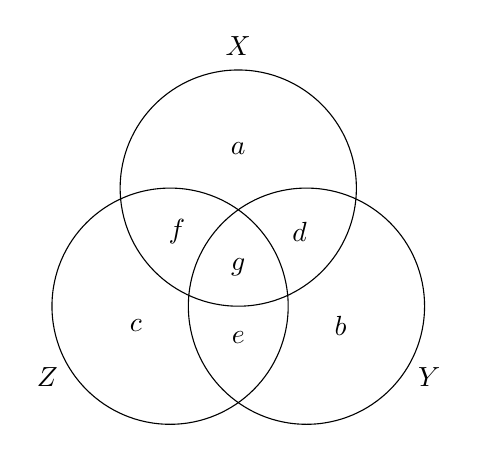
\begin{tikzpicture}
    % circles
    \draw (90:1) circle (1.5);
    \draw (210:1) circle (1.5);
    \draw (330:1) circle (1.5);

    % labels
    \node at (90:2.8) {$X$};
    \node at (330:2.8) {$Y$};
    \node at (210:2.8) {$Z$};
    
    \node at (90:1.5) {$a$};
    \node at (330:1.5) {$b$};
    \node at (210:1.5) {$c$};
    \node at (30:.9) {$d$};
    \node at (270:.9) {$e$};
    \node at (150:.9) {$f$};
    \node at (0:0) {$g$};
  \end{tikzpicture}
  \caption{Partition of $X \cup Y \cup Z$.  The quantities $a,b,c,d,e,f,g$
    represent the cardinalities of each disjoint set as shown.}
  \label{fig:partition}
\end{figure}

A related dissimilarity is the normalised symmetric difference,
$\delta_{\symdif} \colon 2^{\dset} \times 2^{\dset} \to \mathbb{R}^{\geq 0}$,
defined as:
\begin{equation*}
  \delta_{\symdif_n}(X,Y) =
  \begin{cases}
    \displaystyle \frac{|X \symdif Y|}{|X \cup Y|} & \text{if $X \cup Y \neq
      \emptyset$}, \\
    0 & \text{otherwise,}
  \end{cases}
\end{equation*}
for all $X,Y \in 2^{\dset}$.

\begin{thm}
  The normalised symmetric difference is a metric on $2^{\dset}$.
\end{thm}

The following proof was presented in \citep{yianilos91}, with some errors.  We
reproduce the proof here with the errors corrected.

\begin{proof}
  It is easy to see the function is nonnegative, symmetric and that
  $\delta_{\symdif_n}(X,Y)=0$ if and only if $X=Y$ for all $X,Y \in 2^{\dset}$
  so we will show that the triangle inequality holds which is:
  \begin{equation*}
    \frac{|X \symdif Y|}{|X \cup Y|} + \frac{|Y \symdif Z|}{|Y \cup Z|} \geq
    \frac{|X \symdif Z|}{|X \cup Y|}
  \end{equation*}
  or, equivalently:
  \begin{equation}
    \label{eq:tri-inequality}
    1 - \frac{|X \cap Y|}{|X \cup Y|} +
    1 - \frac{|Y \cap Z|}{|Y \cup Z|} \geq
    1 - \frac{|X \cap Z|}{|X \cup Z|}.
  \end{equation}

  We partition $X \cup Y \cup Z$ into disjoint subsets as shown in
  Figure~\ref{fig:partition} and let
  \begin{align*}
    a = |X \setminus (Y \cup Z)|,&\qquad
    b = |Y \setminus (X \cup Z)|,\\
    c = |Z \setminus (X \cup Y)|,&\qquad
    d = |(X \cap Y) \setminus Z|.\\
    e = |(Y \cap Z) \setminus X|.&\qquad
    f = |(Z \cap X) \setminus Y|.\\
    g = |X& \cap Y \cap Z|,
  \end{align*}
  and for convenience we let
  \begin{equation*}
    \xi  = |X \cup Y \cup Z|.
  \end{equation*}

  We can now write equation~(\ref{eq:tri-inequality}) as
  \begin{equation*}
    1 - \frac{d+g}{\xi -c} + 1 - \frac{e+g}{\xi -a} \geq 1 - \frac{f+g}{\xi -b}
  \end{equation*}
  which can be rewritten as
  \begin{equation*}
    \frac{d+g}{\xi -c} + \frac{e+g}{\xi -a} \leq \frac{f+g}{\xi -b} + 1.
  \end{equation*}

  Removing $b$ from the denominators on the LHS can only make the LHS
  greater, so it is sufficient to show that
  \begin{equation*}
    \frac{d+g}{\xi -b-c} + \frac{e+g}{\xi -a-b} \leq \frac{f+g}{\xi -b} + 1.
  \end{equation*}

  Now if we replace $1$ with $\frac{\xi -a-b-c}{\xi -a-b-c}$ on the RHS and add
  the fractions on the LHS we get
  \begin{multline*}
    \frac{(\xi -a-b)(d+g)+(\xi -b-c)(e+g)}{(\xi -b-c)(\xi -a-b)}\\
    \leq \frac{(\xi -a-b-c)(\xi -b)+(\xi -a-b-c)(f+g)}{(\xi -b)(\xi -a-b-c)}
  \end{multline*}
  which when we expand the denominators becomes
  \begin{multline*}
    \frac{(\xi -a-b)(d+g)+(\xi -b-c)(e+g)}{\xi ^2-\xi a-2\xi b-\xi c+ab+bc+b^2+ac}\\
    \leq \frac{(\xi -a-b-c)(\xi -b)+(\xi -a-b-c)(f+g)}{\xi ^2-\xi a-2\xi b-\xi c+ab+bc+b^2}.
  \end{multline*}
  Notice that the denominator on the LHS is equal to the denominator on the
  RHS with the addition of $ac$ so it cannot be less.  It is therefore
  sufficient to show that
  \begin{multline*}
    (\xi -a-b)(d+g)+(\xi -b-c)(e+g)\\
    \leq (\xi -a-b-c)(\xi -b)+(\xi -a-b-c)(f+g).
  \end{multline*}

  Starting with the LHS we have
  \begin{align*}
    &(\xi -a-b)(d+g)+(\xi -c-b)(e+g)\\
    &= (\xi -a-b-c)(d+g)+c(d+g)+(\xi -a-b-c)(e+g)+a(e+g)\\
    &\leq (\xi -a-b-c)(d+g)+c(\xi -a-b-c)\\
    &\qquad\qquad+(\xi -a-b-c)(e+g)+a(\xi -a-b-c)\\
    &= c(\xi -a-b-c)+(\xi -a-b-c)(d+e+g)\\
    &\qquad\qquad+g(\xi -a-b-c)+a(\xi -a-b-c)\\
    &\leq c(\xi -a-b-c)+(\xi -a-b-c)^2+g(\xi -a-b-c)+a(\xi -a-b-c)\\
    &= (\xi -a-b-c)(\xi -b)+g(\xi -a-b-c)\\
    &\leq (\xi -a-b-c)(\xi -b) + (f+g)(\xi -a-b-c).
  \end{align*}
\end{proof}

\subsubsection{Hausdorff distance}
\label{sec:hausdorff-distance}

\begin{figure}
  \centering
  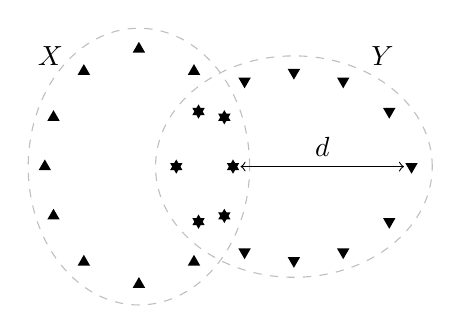
\begin{tikzpicture}[
    ]

    \draw [dashed,faint] (-2.8em,0) ellipse (4em and 5em);
    \draw [dashed,faint] (2.8em,0) ellipse (5em and 4em);

    % set 1 primary markers
    \begin{scope}[xshift=-2.8em,scale=0.85]
      \foreach \theta in {0,30,...,330} {
        \pgfmathparse{(4*5)/sqrt((5*cos(\theta))^2+(4*sin(\theta))^2)}
        \node [setnode1] (1set\theta) at (\theta:\pgfmathresult em) {};
      }
    \end{scope}
    % set 2 markers
    \begin{scope}[xshift=-2.8em,scale=0.85]
      \foreach \theta in {0,30,330} {
        \pgfmathparse{(4*5)/sqrt((5*cos(\theta))^2+(4*sin(\theta))^2)}
        \node [setnode2] at (\theta:\pgfmathresult em) {};
      }
    \end{scope}

    % set 2 primary markers
    \begin{scope}[xshift=2.8em,scale=0.85]
      \foreach \theta in {0,30,...,330} {
        \pgfmathparse{(5*4)/sqrt((4*cos(\theta))^2+(5*sin(\theta))^2)}
        \node [setnode2] (2set\theta) at (\theta:\pgfmathresult em) {};
      }
    \end{scope}
    % set 1 markers
    \begin{scope}[xshift=2.8em,scale=0.85]
      \foreach \theta in {150,180,210} {
        \pgfmathparse{(5*4)/sqrt((4*cos(\theta))^2+(5*sin(\theta))^2)}
        \node [setnode1] at (\theta:\pgfmathresult em) {};
      }
    \end{scope}

    \draw [symdist] (2set0) -- node[auto,swap] {$d$} (1set0);

    % labels
    \node at (-6em,4em) {$X$};
    \node at (6em,4em) {$Y$};
  \end{tikzpicture}
  \caption{$X$ and $Y$ are sets with elements labelled by \tikzuptriangle ~and
    \tikzupdtriangle ~respectively.  Elements in both sets are labelled with
    \tikzbotriangle .  The Hausdorff distance between $X$ and $Y$ is,
    informally, the greatest distance one must travel if starting from a point
    in one set and travelling to the closest point in the other.  This
    distance is marked by $d$ in the diagram.}
  \label{fig:haussdorf}
\end{figure}

Let $(M,d)$ be a metric space and $\mathcal{M}=2^M \setminus \{\emptyset\}$.
The Hausdorff distance, $\delta_{H} \colon \mathcal{M} \times \mathcal{M} \to
\mathbb{R}^{\geq 0}$, is defined as:
\begin{equation*}
  \delta_{H}(X,Y) = \max\left(\max_{x \in X} \min_{y \in Y} d(x,y),
                             \max_{y \in Y} \min_{x \in X} d(x,y)\right), 
\end{equation*}
for all $X,Y \in \mathcal{M}$.  The Hausdorff distance is a metric on
$\mathcal{M}$ \citep{braun2003geometry}.  This distance is illustrated in
Figure~\ref{fig:haussdorf} by showing the Hausdorff distance between two sets
with elements in a metric space.  In Chapter~\ref{cha:sum-squar-clust} we
present a new metric on $\mathcal{M}$.

\subsubsection{Linkage functions}
\label{sec:linkage-functions}

We conclude by remarking that the linkage functions, which are used in
hierarchical clustering, the topic of Section~\ref{sec:hier-clust-meth}, are
not generally metrics.  For a metric space, $(M,d)$, and $\mathcal{M}=2^M
\setminus \emptyset$, the \textit{single-linkage distance}, $\delta_{SL}
\colon \mathcal{M} \times \mathcal{M} \to \mathbb{R}^{\geq 0}$ is defined as:
\begin{equation*}
  \delta_{SL}(X,Y) = \min_{x \in X, y \in Y} d(x,y),
\end{equation*}
for all $X,Y \in \mathcal{M}$.  While single-linkage is a simple and intuitive
distance between sets, it is not a metric since distinct sets can have a
distance of zero.  The \textit{complete-linkage} and \textit{average-linkage}
dissimilarities are, in fact, not even distances.  These measures will be
discussed further in Section~\ref{sec:hier-clust-meth}.

% \subsection{Multiset datasets}
% \label{sec:multiset-datasets}

% It is tempting to think of a dataset and a metric defined on its elements as a
% metric space, but this is not necessarily correct.  The reason is that,
% contrary to the name, a dataset is not usually a set but a multiset.  Consider
% a dataset consisting of only the heights of some population of humans.
% Depending on the precision of the measurements taken, it would generally be
% expected that multiple subjects share the same height.  In order to have these
% observations in a set, some unique integer---an experiment number, say---would
% need to be attached to each observation.  But then the metric condition that
% $d(x,y)=0$ only if $x=y$ would be violated---in fact we would have only a
% \textit{pseudometric}.  We can get a proper metric if we define an equivalence
% relation $x \sim y$ if $d(x,y)=0$.  Then $(\dset/\sim,d)$ is a metric space.

% Most of the time we do not need to worry about this.  From now on a dataset,
% $\dset$, will implicitly mean $\dset/\sim$ as defined above unless stated
% otherwise.  Occasionally. though, it will be useful or necessary to consider
% the multiset $(\dset,\mu_{\dset})$ where $\dset$ is the underlying set, and
% $\mu_{\dset} \colon \dset \to \mathbb{N}_1$---a map from $\dset$ to the
% (nonzero) natural numbers---is called the membership function and tells us how
% many times an element appears in the multiset.

% A further generalisation is then possible: we can relax the definition of the
% membership function to $\mu_{\dset} \colon \dset \to \mathbb{R}_1$---a map
% from $\dset$ to the positive real numbers.  The dataset is then a fuzzy
% multiset.  Such datasets have been used in document clustering applications,
% for example in \citep{miyamoto2003information}, where objects can appear
% multiple times with a certain probability attached.  If the membership
% function if $\mu_{\dset} \colon \dset \to \mathbb{R}_1 \cap [0,1]$ then
% $(\dset,\mu_{\dset})$ is called a fuzzy set
% \citep{zadeh1965fuzzy,gottwald2010fuzzy}.

\section{Partitions}
\label{sec:partitions}

In this section we look at the properties of partitions of sets, how we can
compare partitions and how we can find partitions.  Throughout, we assume that
$n > 0$ and refer to a set of $n$ elements as an \textit{$n$-set}.

\subsection{The space of partitions}
\label{sec:space-partitions}

Given an $n$-set $\dset$, a $k$-partition $\clus = \{C_1,C_2,\dotsc,C_k\}$ of
$\dset$ is a set of $k \in \{1,\dotsc,n\}$ nonempty, pairwise-disjoint subsets
of $\dset$ such that $C_1 \cup C_2 \cup \dotsb \cup C_k = \dset$.  Following
common practice, we will refer to the elements of $\clus$ as
\textit{clusters}.

\begin{figure}
  \centering
  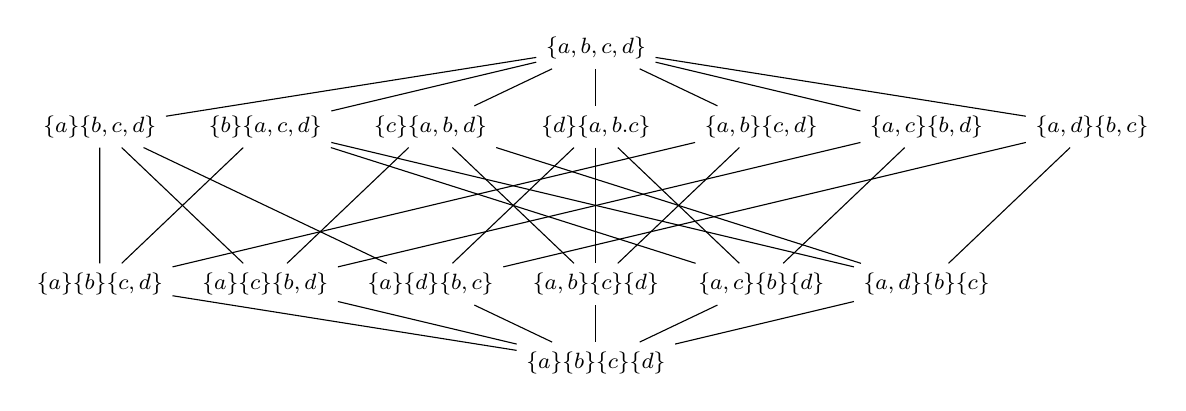
\begin{tikzpicture}[
    xscale=2.1, font=\footnotesize]

    % vertices
    
    \node (0) at (0,0) {$\{a,b,c,d\}$};

    \node (10) at (-3,-1) {$\{a\}\{b,c,d\}$};
    \node (11) at (-2,-1) {$\{b\}\{a,c,d\}$};
    \node (12) at (-1,-1) {$\{c\}\{a,b,d\}$};
    \node (13) at (0,-1) {$\{d\}\{a,b.c\}$};
    \node (14) at (1,-1) {$\{a,b\}\{c,d\}$};
    \node (15) at (2,-1) {$\{a,c\}\{b,d\}$};
    \node (16) at (3,-1) {$\{a,d\}\{b,c\}$};

    \node (20) at (-3,-3) {$\{a\}\{b\}\{c,d\}$};
    \node (21) at (-2,-3) {$\{a\}\{c\}\{b,d\}$};
    \node (22) at (-1,-3) {$\{a\}\{d\}\{b,c\}$};
    \node (23) at (0,-3) {$\{a,b\}\{c\}\{d\}$};
    \node (24) at (1,-3) {$\{a,c\}\{b\}\{d\}$};
    \node (25) at (2,-3) {$\{a,d\}\{b\}\{c\}$};

    \node (3) at (0,-4) {$\{a\}\{b\}\{c\}\{d\}$};

    % edges

    \draw (0) to (10);
    \draw (0) to (11);
    \draw (0) to (12);
    \draw (0) to (13);
    \draw (0) to (14);
    \draw (0) to (15);
    \draw (0) to (16);

    \draw (10) to (20);
    \draw (10) to (21);
    \draw (10) to (22);
    \draw (11) to (20);
    \draw (11) to (24);
    \draw (11) to (25);
    \draw (12) to (21);
    \draw (12) to (23);
    \draw (12) to (25);
    \draw (13) to (22);
    \draw (13) to (23);
    \draw (13) to (24);
    \draw (14) to (20);
    \draw (14) to (23);
    \draw (15) to (21);
    \draw (15) to (24);
    \draw (16) to (22);
    \draw (16) to (25);

    \draw (20) to (3);
    \draw (21) to (3);
    \draw (22) to (3);
    \draw (23) to (3);
    \draw (24) to (3);
    \draw (25) to (3);
  \end{tikzpicture}
  \caption{The Hasse diagram of the lattice of partitions of a set,
    $\dset=\{a,b,c,d\}$ \citep{meila-2005}.  Each vertex in the graph is a
    partition $\{C_1,\dotsc,C_k\}$ of $\dset$ which we denote by
    $C_1,\dotsc,C_k$ for clarity.}
  \label{fig:lattice}
\end{figure}

Let $\parts_{\dset}$ be the set of all partitions of $\dset$ and $\clus,\clus'
\in \parts_{\dset}$.  The partition $\clus$ is called a \textit{refinement} of
$\clus'$ if every element of $\clus$ is a subset of some element of $\clus'$.
We can then say that $\clus$ is \textit{finer-than-or-equal-to} $\clus'$,
which we notate $\clus \leq \clus'$ (or that $\clus'$ is
\textit{coarser-than-or-equal-to} $\clus$).  The relation $\leq$ imposes a
partial order on the elements of $\parts_{\dset}$.

The partially-ordered set $(\parts_{\dset},\leq)$ is called the
\textit{lattice of partitions} and can be represented in terms of a graph
called the \textit{Hasse diagram} associated with $\parts_{\dset}$.  The
vertex set of that graph is $\parts_{\dset}$ and its arc set consists of the
pairs $(\clus_1,\clus_2) \in \parts_{\dset} \times \parts_{\dset}$ such that
$\clus_2 < \clus_1$ and there exists no $\clus_3 \in \parts_{\dset}$ such that
$\clus_2 < \clus_3 < \clus_1$.  Informally, this means that $\clus_2$ can be
obtained by bisecting one cluster of $\clus_1$.

The Hasse diagram of the set $\dset = \{a,b,c,d\}$ is presented in
Figure~\ref{fig:lattice}.  The partition at the top is the coarsest partition
(a 1-partition) and the partition at the bottom is the finest partition (an
$n$-partition).

As this example suggests, a set can potentially support a very large number of
partitions.  For an $n$-set $\dset$ the cardinality of $\parts_{\dset}$ is
given by the \textit{Bell number} $B_n$
\citep{bell1934exponential,stanley2000enumerative} where $B_0=1$ and
\begin{equation*}
  B_n = \sum_{l=0}^{n-1} B_l \binom{n-1}{l} \qquad \text{for $n \geq 1$}.
\end{equation*}
Alternatively, $B_n$ is given by Dobi\'{n}ski's formula
\citep{dobinski1877summation}:
\begin{equation*}
  B_n = \frac{1}{e} \sum_{l=0}^{\infty} \frac{l^n}{l!} \qquad \text{for $n
    \geq 0$}.
\end{equation*}
We illustrate the growth of the Bell number in Table~\ref{tab:bell-number}.

\begin{table}
  \centering
  \begin{tabular}{rr}
    \toprule
    $n$ & $B_n$ \\
    \midrule
    5 & 52 \\
    10 & 115,975 \\
    15 & 1,382,958,545 \\
    20 & $5.17 \times 10^{13}$ \\
    25 & $4.64 \times 10^{18}$ \\
    \bottomrule
  \end{tabular}
  \caption{The value of the Bell number, $B_n$, for some selected values of
    $n$.  The value of $B_n$ is equivalent to the number of possible
    partitions of an $n$ element set.}
  \label{tab:bell-number}
\end{table}

\subsubsection{Fuzzy partitions}
\label{sec:fuzzy-partitions}

Partitions can be generalised to fuzzy partitions by letting the clusters be
fuzzy sets.  Fuzzy sets are collections of objects where each member of a
collection has a grade of membership associated to it \citep{zadeh1965fuzzy}.
Sets are a special case where the grades of membership are binary---objects
are either members of a set or they are not.  Fuzzy sets and partitions have
many applications including classification of data in the natural sciences
where membership is not precisely defined.

Formally, a fuzzy set is an ordered pair $(C,\mu_{C})$ consisting of an
underlying set $C$ and a membership function $\mu_{C} \colon C \to [0,1]$.
For some fuzzy set $(C,\mu_C)$ and element $x \in C$ $\mu_C(x) = 1$ means $x$
is a full member, $\mu_C(x) = 0$ means $x$ is not a member and $0 < \mu_C(x) <
1$ means $x$ is a fuzzy member.  If $\mu_C(x) = 0$ or $1$ for all $x \in C$
then the object is called by contrast a \textit{crisp set} and may be handled
by ordinary set theory \cite{zadeh1965fuzzy,klir1995fuzzy}.

A \textit{$k$-fuzzy-partition} of an $n$-set $\dset$ is a set of $k \in
\{1,\dotsc,n\}$ fuzzy sets: \[\{(C_1,\mu_1),(C_2,\mu_2),\dotsc,(C_k,\mu_k)\}\]
where $C_1 \cup \dotsb \cup C_k = \dset$, $C_i \neq \emptyset$ for all $i \in
\{1,\dotsc,k\}$ and $\sum_{i=1}^{k} \mu_i(x) = 1$ for all $x \in \dset$.  Note
that the underlying sets of the fuzzy sets $(C_i,\mu_i)$ are not necessarily
pairwise disjoint, so elements can belong to more than one cluster.

\subsection{Comparing partitions}
\label{sec:comparing-partitions}

An attractive way to find partitions of a set is by means of a partitional
clustering method.  Many methods exist---we will review some in
Section~\ref{sec:part-clust-algor}---and, depending on their respective
approach to the problem, they all tend to produce different partitions.  To
further complicate matters, some methods are nondeterministic so can
potentially produce different partitions each time they are used.

For the purposes of comparing and assessing clustering methods it is therefore
useful to be able to compare partitions.  Many measures have been devised for
this purpose, including similarity measures and dissimilarity measures, of
which some are metrics.  Existing methods fall into four main categories; for
two partitions $\clus_1$ and $\clus_2$ of a set $\dset$, these are:
\begin{description}
\item[Pair counting] which measures the agreement and disagreement between
  $\clus_1$ and $\clus_2$ by means of counting pairs of element in $\dset$,
\item[Set matching] which ``matches'' clusters in $\clus_1$ with clusters in
  $\clus_2$ and measures the similarity between matched sets,
\item[Information theoretic] which uses information theory to measure the
  information and mutual information contained in $\clus_1$ and $\clus_2$,
\item[Density profile] which takes into account the values of the data when
  computing the measure.
\end{description}

We will review measures belonging to the first three categories in this
section.  The fourth category consists of a single measure called ADCO which
we will analyse in Chapter~\ref{cha:sum-squar-clust}.

To be able to describe the measures in detail, we need to introduce some more
terminology.  Let $\dset = \{x_1,x_2,\dotsc,x_n\}$ be an $n$-set with $n \geq
2$ and again, as before, let $\clus_1 = \{C_{11},C_{12},\dotsc,C_{1k}\}$ and
$\clus_2 = \{C_{21},C_{22},\dotsc,C_{2k'}\}$ be two partitions of $\dset$ with
$k$ and $k'$ clusters, respectively.  We denote, for some $x \in \dset$, and a
partition, $\clus$, of $\dset$, the cluster in $\clus$ that contains $x$ by
$\clus(x)$.  The \textit{confusion matrix} associated with $\clus_1$ and
$\clus_2$ is the $k \times k'$ matrix $[n_{ij}]$ where $n_{ij} = |C_{1i} \cap
C_{2j}|$.  It is used for the calculation of both pair counting and set
matching measures.

To illustrate these definitions and the comparison measures we review below,
we will use two example partitions $\clus^*_1$ and $\clus^*_2$ of the set
$\dset^* = \{1,\dotsc,9\}$ throughout this section:
\begin{equation}
  \label{eq:example-parts}
  \clus^*_1 = \{C^*_{11},C^*_{12},C^*_{13}\},\qquad
  \clus^*_2 = \{C^*_{21},C^*_{22},C^*_{23},C^*_{24}\}
\end{equation}
where
\begin{align*}
  C^*_{11}&=\{1,2,3\},\quad C^*_{12}=\{4,5,6\},\quad C^*_{13}\{7,8,9\} \quad \text{and}\\
  C^*_{21}&=\{1,4\},\quad C^*_{22}=\{2,3,6\},\quad C^*_{23}=\{5,8\},\quad C^*_{24}\{7,9\}.
\end{align*}
Then, for example, we have $\clus^*_1(3) = C^*_{11}$, and the confusion matrix
associated with $\clus^*_1$ and $\clus^*_2$ is:
\begin{equation*}
  [n_{ij}]^*=\left[
  \begin{matrix}
    1 & 2 & 0 & 0 \\
    1 & 1 & 1 & 0 \\
    0 & 0 & 1 & 2
  \end{matrix}
  \right]
\end{equation*}

\subsubsection{Pair counting}
\label{sec:pair-counting}

There are $\binom{n}{2}$ distinct pairs of elements in $\dset$.  For each
distinct pair $(a,b) \in \dset \times \dset$ one of the following is true:
\begin{align*}
\clus_1(a)=\clus_1(b) &\text{ and } \clus_2(a)=\clus_2(b),\\
\clus_1(a)\neq \clus_1(b) &\text{ and } \clus_2(a)\neq \clus_2(b),\\
\clus_1(a)=\clus_1(b) &\text{ and } \clus_2(a)\neq \clus_2(b),\\
\clus_1(a)\neq \clus_1(b) &\text{ and } \clus_2(a)=\clus_2(b).
\end{align*}
Counting the number of element in each category gives us four counts which are
defined formally as:
\begin{align*}
  N_{11} &= |\{(a,b) \in \dset \times \dset \colon
              \clus_1(a)=\clus_1(b) \text{ and } \clus_2(a)=\clus_2(b)
            \}|, \\
  N_{00} &= |\{(a,b) \in \dset \times \dset \colon
              \clus_1(a)\neq\clus_1(b) \text{ and } \clus_2(a)\neq\clus_2(b)
            \}|, \\
  N_{10} &= |\{(a,b) \in \dset \times \dset \colon
              \clus_1(a)=\clus_1(b) \text{ and } \clus_2(a)\neq\clus_2(b)
            \}|, \\
  N_{01} &= |\{(a,b) \in \dset \times \dset \colon
              \clus_1(a)\neq\clus_1(b) \text{ and } \clus_2(a)=\clus_2(b)
            \}|.
\end{align*}
The size of $N_{11}$ and $N_{00}$ are considered to be measurements of
\textit{agreement} between $\clus_1$ and $\clus_2$, while $N_{10}$ and
$N_{01}$ are considered measurements of \textit{disagreement}.

The measures based on pair counting can all be expressed in terms of these
four counts.  Clearly \[N_{11}+N_{00}+N_{10}+N_{01} = \binom{n}{2}\] is always
satisfied.  The quantities $N_{11},N_{00},N_{10}$ and $N_{01}$ can all be
obtained from the confusion matrix using the following formul\ae
\citep{hubert-arabie-1985}:
\begin{align*}
  N_{11} &= \frac{1}{2} \sum_{i=1}^{k} \sum_{j=1}^{k'} n_{ij}(n_{ij}-1),\\
  N_{00} &= \frac{1}{2} \left(n^2 + \sum_{i=1}^{k} \sum_{j=1}^{k'} n_{ij}^2
                             - \sum_{i=1}^{k}
                                \left(\sum_{j=1}^{k'} n_{ij} \right)^2
                             - \sum_{j=1}^{k'}
                                \left(\sum_{i=1}^{k} n_{ij} \right)^2
                       \right),\\
  N_{10} &= \frac{1}{2} \left(\sum_{i=1}^{k}
                              \left(\sum_{j=1}^{k'} n_{ij} \right)^2
                             - \sum_{i=1}^{k} \sum_{j=1}^{k'} n_{ij}^2
                       \right),\\
  N_{01} &= \frac{1}{2} \left(\sum_{j=1}^{k'}
                              \left(\sum_{i=1}^{k} n_{ij} \right)^2
                             - \sum_{i=1}^{k} \sum_{j=1}^{k'} n_{ij}^2
                       \right).
\end{align*}
The four counts for our example partitions $\clus^*_1$ and $\clus^*_2$ are:
\begin{equation*}
  N_{11} = 2,\quad
  N_{00} = 23,\quad
  N_{10} = 7,\quad
  N_{01} = 4.
\end{equation*}

One of the simplest pair counting measures between $\clus_1$ and $\clus_2$ is
the widely-used \textit{Rand index} $\partcomparen{R}$ introduced in
\citep{rand-1971} and defined as:
\begin{equation*}
\partcompare{R} = \frac{(N_{11}+N_{00})}{\binom{n}{2}}.
\end{equation*}
The Rand index is a similarity measure with a lower bound of 0 and an upper
bound of 1.  \citet{hubert-arabie-1985} use the following variation:
\[\partcompare{HA} = (N_{11}+N_{00}-N_{10}-N_{01})/\binom{n}{2}.\]

\citet{wallace-1983} introduced two asymmetric measures for comparing
$\clus_1$ and $\clus_2$ defined as:
\begin{equation*}
  \mathcal{W}_{I}(\clus_1,\clus_2) =
  \frac{N_{11}}{\sum_{i=1}^{k} |C_{i1}|(|C_{1i}|-1)/2},
\end{equation*}
and
\begin{equation*}
  \mathcal{W}_{II}(\clus_1,\clus_2) =
  \frac{N_{11}}{\sum_{j=1}^{k'} |C_{2j}|(|C_{2j}|-1)/2}.
\end{equation*}
$\mathcal{W}_{I}$ and $\mathcal{W}_{II}$ represent the probabilities that, for
a pair of elements $(a,b) \in \dset \times \dset$ with
$\clus_1(a)=\clus_1(b)$, we also have $\clus_2(a)=\clus_2(b)$, and vice versa.
A symmetric similarity measure for $\clus_1$ and $\clus_2$ can be obtained by
taking the geometric mean of the Wallace measures:
\begin{equation*}
  \partcompare{F} = \sqrt{\mathcal{W}_{I}(\clus_1,\clus_2)
                          \mathcal{W}_{II}(\clus_1,\clus_2)}.
\end{equation*}
This measure was also introduced independently by Fowlkes and Mallows in
\citep{fowlkes-mallows-1983}.

The \textit{Jaccard coefficient} $\partcomparen{J}$ is another widely-used
similarity measure and is defined, for $\clus_1$ and $\clus_2$, as:
\begin{equation*}
  \partcompare{J} = \frac{N_{11}}{N_{10}+N_{01}+N_{11}}.
\end{equation*}

It should be noted that all measures reviewed so far are similarity measures.
The \textit{Mirkin metric} $\partcomparen{M}$ for measuring dissimilarity
between $\clus_1$ and $\clus_2$ was originally introduced in
\citep{mirkin1996mathematical} and is defined as
\begin{equation*}
  \partcompare{M} = \sum_{i=1}^{k} |C_{1i}|^2 +
                    \sum_{j=1}^{k'} |C_{1j}|^2 +
                    2\sum_{i=1}^{k}\sum_{j=1}^{k'} n_{ij}^2,
\end{equation*}
where $[n_{ij}]$ again denotes the confusion matrix associated with $\clus_1$
and $\clus_2$.  As it turns out, \[\partcompare{M}=2(N_{10}+N_{01}).\] The
closely related measure: \[\partcompare{AB}=(N_{10}+N_{01})/\binom{n}{2}\] is
also a metric on $\parts_{\dset}$ and was used by
\citet{mirkin1970measurement} and \citet{arabie1973multidimensional}.

\begin{table}
  \centering
  \begin{tabular}{lr}
    \toprule
    Name & Measure \\
    \midrule
    Rand index          & $\partcomparest{R} \approx 0.694$ \\
    Wallace measures    & $\mathcal{W}_{I}(\clus^*_1,\clus^*_2) \approx 0.222$ \\
                        & $\mathcal{W}_{II}(\clus^*_1,\clus^*_2) \approx 0.333$ \\
    Fowlkes \& Mallows  & $\partcomparest{F} \approx 0.272$ \\
    Jaccard coefficient & $\partcomparest{J} \approx 0.154$ \\
    Merkin metric       & $\partcomparest{M} = 22.00$ \\
    \bottomrule
  \end{tabular}
  \caption{Various pair counting based measures applied to the example
    partitions $\clus^*_1$ and $\clus^*_2$~\eqref{eq:example-parts}.}
  \label{tab:pair-counting-comparison}
\end{table}

The values of the reviewed pair counting measures when applied to $\clus^*_1$
and $\clus^*_2$ are given in Table~\ref{tab:pair-counting-comparison}.

\subsubsection{Set matching}
\label{sec:set-matching}

Set matching measures for partitions $\clus_1$ and $\clus_2$ are based on
comparisons between matched pairs of clusters.  Each pair to be compared
consists of one element of $\clus_1$ and one of $\clus_2$.  All of the
measures that we review here are based on the confusion matrix, meaning that
they use the cardinality of the intersection between two clusters as a
similarity measure.  The differences between the measures are essentially due
to the way that they find the matched pairs of clusters for comparison.

As before, let $\dset$ be an $n$-set and let $\clus_1 =
\{C_{11},\dotsc,C_{1k}\}$ and $\clus_2 = \{C_{21},\dotsc,C_{1k'}\}$, where
$k,k' \geq 1$, denote two partitions of $\dset$.  Also assume, without loss of
generality, that $k' \geq k$.  Then, a \textit{matching} between $\clus_1$ and
$\clus_2$ is a function $\sigma \colon \{1,\dotsc,k\} \to \{1,\dotsc,k'\}$.

\begin{figure}
  \centering
  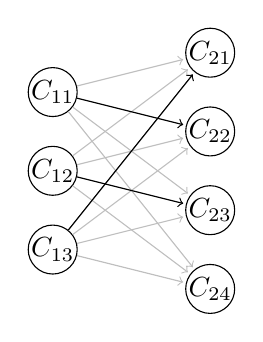
\begin{tikzpicture}[
    % >=stealth,
    % clus/.style={circle,draw=black,inner sep=0,minimum size=5mm},
    % dist/.style={->,shorten >=2pt},
    % faint/.style={dist,gray!50},
    nonmatch/.style={dist,faint},
    match/.style={dist,black}
    ]

    \node [clus] (c11) at (0,1) {$C_{11}$};
    \node [clus] (c12) at (0,0) {$C_{12}$};
    \node [clus] (c13) at (0,-1) {$C_{13}$};

    \node [clus] (c21) at (2,1.5) {$C_{21}$};
    \node [clus] (c22) at (2,.5) {$C_{22}$};
    \node [clus] (c23) at (2,-.5) {$C_{23}$};
    \node [clus] (c24) at (2,-1.5) {$C_{24}$};

    % join them all
    \foreach \x in {1,2,3} {
      \foreach \y in {1,2,3,4} {
        \draw [nonmatch] (c1\x) to (c2\y);
      }
    }

    % matches
    \draw [match] (c11) to (c22);
    \draw [match] (c12) to (c23);
    \draw [match] (c13) to (c21);
  \end{tikzpicture}
  \caption{The clusters belonging to two partitions $\{C_{11},\dotsc,C_{13}\}$
    and $\{C_{21},\dotsc,C_{24}\}$ are shown with all similarities between
    pairs shown in grey.  The black lines represent one possible matching
    between the clusters.  In this case, the matching is an injection.}
  \label{fig:matching}
\end{figure}

\citet{meila-2001} introduced a set matching measure for measuring the
similarity between $\clus_1$ and $\clus_2$.  It finds a matching $\sigma$
using the following heuristic: let $[n_{ij}]$ be the $k \times k'$ confusion
matrix associated with $\clus_1$ and $\clus_2$.  Compute $n_{ab} = \argmax
\{n_{ij} \colon 1 \leq i \leq k, 1 \leq j \leq k'\}$ and put $\sigma(a) \gets
b$.  Repeat the process for the $(k-1) \times (k'-1)$ submatrix obtained by
deleting row $a$ and column $b$, and so on until $k$ matches have been made.
This process clearly finds an injection for $\sigma$ and then the similarity
of $\clus_1$ and $\clus_2$ based on that matching is:
\begin{equation*}
  \partcompare{H} = \frac{1}{n} \sum_{i=1}^{k} n_{i \sigma(i)}.
\end{equation*}

A second similarity measure on $\parts_{\dset}$, denoted $\partcomparen{L}$
and introduced by \citet{larsen-aone-1999} simply computes a maximal match for
each cluster in $\clus_1$ and $\clus_2$:
\begin{equation*}
  \partcompare{L} = \frac{1}{k} \sum_{i=1}^{k} \max_{1 \leq j \leq k'}
                                             \frac{2n_{ij}}{|C_{1i}|+|C_{2j}|}.
\end{equation*}

A dissimilarity measure $\partcomparen{V}$, which is a metric on
$\parts_{\dset}$, was introduced by \citet{van-dongen-2000}.  This measure,
again, computes maximal matches for each cluster in $\clus_1$ and $\clus_2$:
\begin{equation*}
  \partcompare{V} = 2n - \sum_{i=1}^{k} \max_{1 \leq j \leq k'} n_{ij}
                         \sum_{j=1}^{k'} \max_{1 \leq i \leq k} n_{ij}.
\end{equation*}

A second metric on $\parts_{\dset}$ denoted by $\partcomparen{CE}$ is due to
\citet{meila-2005} and is known by the name \textit{classification error}.
Like $\partcomparen{H}$, this measure computes an injection for $\sigma$, but
instead of using a heuristic finds a globally optimal injection in the set
$S_k$ of all possible injections from $\{1,\dotsc,k\}$ to $\{1,\dotsc,k'\}$:
\begin{equation*}
  \partcompare{CE} = 1 - \frac{1}{n} \max_{\sigma \in S_k}
                                     \sum_{i=1}^{k} n_{i \sigma(i)}.
\end{equation*}
Note that the injection, $\sigma$, can be found in polynomial time.  Also,
\[\partcompare{CE} \leq 1\] for all partitions $\clus_1$ and $\clus_2$ of
$\dset$.  The values of the set matching measures when applied to our example
partitions $\clus^*_1$ and $\clus^*_2$ are given in
Table~\ref{tab:set-matching-comparison}.

\begin{table}
  \centering
  \begin{tabular}{lr}
    \toprule
    Name & Measure \\
    \midrule
    Meilă \& Heckerman   & $\partcomparest{H} \approx 0.556$ \\
    Larsen \& Aone       & $\partcomparest{L} \approx 0.622$ \\
    Van Dongen metric    & $\partcomparest{V} = 7.000$ \\
    Classification Error & $\partcomparest{CE} \approx 0.445$ \\
    
    \bottomrule
  \end{tabular}
  \caption{Various set matching based measures applied to the example
    partitions $\clus^*_1$ and $\clus^*_2$~\eqref{eq:example-parts}.}
  \label{tab:set-matching-comparison}
\end{table}

\citet{meila-2007} and \citet{bae2010comparison} point out that all of these
measures suffer from the so-called ``problem of matching'' which we will now
illustrate.  Given a partition $\clus=\{C_1,\dotsc,C_k\}$ with $k\geq 2$
equally sized clusters, we can obtain a partition $\clus'$ from $\clus$ by
moving a fraction $f$ of the objects from each cluster $C_{i}$ to $C_{i+1}$,
with the indices taken$\mod k$.  We can obtain a further partition $\clus''$
from $\clus$ by taking the same fraction from each cluster in $C \in \clus$
and distributing the objects evenly among all other clusters in $\clus
\setminus \{C\}$.  Our intuition would be that the similarity between $\clus$
and $\clus'$ is not the same as the similarity between $\clus$ and $\clus''$.
However,
\begin{align*}
  \partcomparep{H} = \partcomparepp{H},&\quad
  \partcomparep{L} = \partcomparepp{L},\\
  \partcomparep{V} = \partcomparepp{V},&\quad
  \partcomparep{CE} = \partcomparepp{CE}
\end{align*}
whenever $0< f < 1/2$.

To give a numerical example, let $\dset = \{1,\dotsc,15\}$,
\begin{equation*}
  \clus = \{\{1,2,3,4,5\},\{6,7,8,9,10\},\{11,12,13,14,15\}\}
\end{equation*}
be a partition of $\dset$ and $f = 2/5$.  Then
\begin{equation*}
\clus' = \{\{1,2,3,14,15\},\{6,7,8,4,5\},\{11,12,13,9,10\}\}
\end{equation*}
and
\begin{equation*}
\clus'' = \{\{1,2,3,9,14\},\{6,7,8,4,15\},\{11,12,13,5,10\}\}
\end{equation*}
are partitions of $\dset$ obtained from $\clus$ as described above.  In this
case we have
\begin{align*}
  \partcomparep{H} = \partcomparepp{H} = 3/5,&\quad
  \partcomparep{L} = \partcomparepp{L} = 3/5,\\
  \partcomparep{V} = \partcomparepp{V} = 12,&\quad
  \partcomparep{CE} = \partcomparepp{CE} = 2/5.
\end{align*}

\subsubsection{Information theoretic}
\label{sec:inform-theor}

Two measures which use information theory are \textit{Normalized Mutual
  Information} \citep{fred-jain-2003} and \textit{Variation of Information}
\citep{meila-2007}.  For the remainder of this section we will focus on the
latter and refer the reader to \citep{fred-jain-2003} for details on the
former.

Variation of Information is based on both how much information is contained in
each partition and how much information one partition contains about the other
(their mutual information).

Let $\clus = \{C_{1},\dotsc,C_{k}\}$, where $k \geq 1$, be partition of an
$n$-set $\dset$.  Then the \textit{information} contained in $\clus$ is
measured by:
\begin{equation}
  \label{eq:entropy}
  H(\clus) = -\sum_{i=1}^{k} P_{\clus}(i) \log_b P_{\clus}(i),
\end{equation}
where
\begin{equation*}
  P_{\clus}(i) = \frac{|C_{i}|}{k}, \qquad \text{for $i = 1,\dotsc,k$}.
\end{equation*}
Informally, $P_1(i)$, is the probability that an object picked randomly from
$\dset$ is in cluster $C_{1i}$.  This measure is sometimes called
\textit{entropy}.  The base of the logarithm determines the unit of
information; for example, the bases $b=2,b=e$ and $b=10$ give the information
in so-called \textit{bits}, \textit{nits} and \textit{Hartleys}, respectively
\citep[see][]{kullback68information}.

Now, with $\clus_1 = \{C_{11},\dotsc,C_{1k}\}$ and $\clus_2 =
\{C_{21},\dotsc,C_{1k'}\}$, where $k,k' \geq 1$, the mutual information,
$I(\clus_1,\clus_2)$, between $\clus_1$ and $\clus_2$ is given by:
\begin{equation}
  \label{eq:mutualinf}
  I(\clus_1,\clus_2) = \sum_{i=1}^{k} \sum_{i=1}^{k'}
  P_{12}(i,j) \log_b \frac{P_{12}(i,j)}{P_{\clus_1}(i)P_{\clus_2}(j)},
\end{equation}
where
\begin{equation*}
  P_{12}(i,j) = \frac{|C_{1i} \cap C_{2j}|}{n}, \qquad \text{for $i =
    1,\dotsc,k,j = 1,\dotsc,k'$}.
\end{equation*}
Informally, $P_{12}(i,j)$ is the probability that an object picked randomly
from $\dset$ is in both $C_{1i}$ and $C_{2j}$.

The \textit{Variation of Information}, $\partcomparen{VI}$, between $\clus_1$
and $\clus_2$ is then defined as:
\begin{equation*}
  \partcompare{VI} = H(\clus_1) + H(\clus_2) - 2I(\clus_1,\clus_2).
\end{equation*}

As it turns out, $\Delta_{\mathcal{VI}}$ is a metric on $\parts_{\dset}$ and
has some attractive properties.  These include that it is $n$-invariant,
meaning its value depends only on the relative sizes of the clusters in
$\clus_1$ and $\clus_2$ and not on the size of $n$.  Further, it is bounded
for all $n$ by
\begin{equation*}
  \partcompare{VI} \leq \log_b n.
\end{equation*}
Finally, if $\max(k,k') \leq k^*$ where $k^* \leq \sqrt{n}$ then
\begin{equation*}
  \partcompare{VI} \leq 2 \log_b k^*
\end{equation*}
holds.

\begin{table}
  \centering
  \begin{tabular}{lr}
    \toprule
    Name & Measure \\
    \midrule
    Information & $H(\clus^*_1) \approx 1.585$ \\
                & $H(\clus^*_2) \approx 1.975$ \\
    Mutual information & $I(\clus^*_1,\clus^*_2) \approx 0.834$ \\
    Variation of Information & $\partcomparest{VI} \approx 1.891$
    \\
    \bottomrule
  \end{tabular}
  \caption{Variation of Information and its components applied to the example
    partitions $\clus^*_1$ and $\clus^*_2$~\eqref{eq:example-parts} using base
    2 for the logarithms in equations~\eqref{eq:entropy} and
    \eqref{eq:mutualinf}.}
  \label{tab:vi-comparison}
\end{table}

The values of Variation of Information and its components applied to our
example partitions, $\clus^*_1$ and $\clus^*_2$, are given in
Table~\ref{tab:vi-comparison}.
\\\\
\noindent We conclude this section with mentioning a further measure called
ADCO, which is a density profile based measure.  We will save discussion of
this measure until we introduce our own Assignment Metric later since these
two metrics share a unique feature possessed by no other measure discussed in
this section.  Namely, they take into account that the partitions to be
compared are partitions of a dataset themselves, with elements that have a
metric defined on them.

\section{Partitional clustering}
\label{sec:part-clust-algor}

The problem of finding meaningful partitions of a dataset is called
\textit{partitional clustering}.  Broadly speaking, the applications of
partitional clustering fall into two categories: \textit{data reduction} and
\textit{object classification}.

Data reduction may be necessary when a dataset is large and it is deemed that
only an essence of the data is wanted for a particular application.  For
example, if geographical data is to be displayed on a map then a large dataset
may not be desirable due to the visual clutter it would create.  Clustering
can be used to reduce the dataset into a more visually appealing and usable
subset.

Object classification is concerned with grouping data into a number of
classes.  For example, given a dataset obtained by market research one may
wish to find different classes of consumers in order to observe their habits
and predict future behaviour.  A further example is document clustering is an
important area concerned with clustering on datasets consisting of objects
written in a natural language.  Search engines such as those found on the
World Wide Web use document clustering to suggest, among other things,
``similar'' documents to the one a user is currently interested in
\citep{steinbach2000comparison}.

\subsection{Criteria}
\label{sec:criteria}

Informally, a meaningful partition of a dataset $(D,d)$ is one which contains
clusters that are homogeneous---meaning objects belonging to the same cluster
are similar---and well-separated---meaning objects belonging to different
clusters are dissimilar, according to $d$.

The task of judging a particular partition of a dataset based on these
informal standards is often a highly subjective one but, nevertheless, many
objective criteria have been devised for the purposes of automatic clustering.
The aim of a partitional clustering algorithm is to find a globally optimal
solution, that is a partition which has maximum homogeneity or separation or
both, according to a particular criterion.

\subsubsection{Dissimilarity based criteria}
\label{sec:diss-based-crit}

The most general criteria for homogeneity and separation are defined only
using dissimilarities.  To make this more precise, let $\dset$ be an $n$-set
with $n\geq 1$, $d \colon \dset \times \dset \to \mathbb{R}^{\geq 0}$ be a
dissimilarity on $\dset$ and $C \subseteq \dset$ be some cluster.
\\\\
\noindent Criteria that measure the homogeneity of $C$ include the
\textit{diameter} of $C$, which is defined as the maximum dissimilarity
between two members of $C$:
\begin{equation*}
  \max_{x,y \in C} d(x,y),
\end{equation*}
the \textit{radius} of $C$, which is defined as the minimum of the maximum
dissimilarities between each member and another member of $C$:
\begin{equation*}
  \min_{x \in C_i} \max_{y \in C} d(x,y)
\end{equation*}
the \textit{star} of $C$, which is defined as the minimum of the sums of
dissimilarities between each member and every other member of $C$:
\begin{equation*}
  \min_{c \in C} \sum_{x \in C} d(x,c),
\end{equation*}
and the \textit{clique} of $C$, which is defined as the sum of dissimilarities
between each pair of members of $C$:
\begin{equation*}
  \sum_{x,y \in C} d(x,y).
\end{equation*}

Criteria that measure the separation of $C$ from every other cluster include
the \textit{split} of $C$, which is defined as the minimum dissimilarity
between a member of $C$ and an element in $\dset \setminus C$:
\begin{equation*}
  \min_{x \in C, y \in \dset \setminus C} d(x,y),
\end{equation*}
and the \textit{cut} of $C$, which is defined as the sum of dissimilarities
between all members of $C$ and all elements in $\dset \setminus C$:
\begin{equation*}
  \sum_{x \in C} \sum_{y \in \dset \setminus C} d(x,y).
\end{equation*}

Dissimilarity based criteria for partitions can then be obtained from the
above measures for clusters by simply taking the sum over all clusters in a
partition.  We call these criteria \textit{sum-of-diameters},
\textit{sum-of-radii}, \textit{sum-of-stars} and so on.  Alternatively one
could simply take the maximum or minimum value, as appropriate, over the
clusters which we would call \textit{max-diameter}, \textit{max-radius},
\textit{min-cut} and so on.  The aim of a clustering method is then to
minimise a criterion for homogeneity or maximise a criterion for separation.

Some criteria for homogeneity are equivalent to criteria for separation.  Most
notably, minimising sum-of-cliques is equivalent to maximising sum-of-cuts.
Such criteria are therefore criteria for both homogeneity and separation.

As it turns out, criteria which only measure one or the other, like min-split
and max-diameter, are often conflicting.  For example, maximising min-split
produces clusters with poor homogeneity, called the \textit{chaining effect},
and minimising max-diameter results in clusters with poor separation, called
the \textit{dissection effect}.  Such criteria are therefore not so useful on
their own, but one way to overcome this problem is to consider a
\textit{bicriterion}, that is simultaneously consider a criterion for
homogeneity and a criterion for separation \citep{delattre1980bicriterion}.

\subsubsection{Scatter matrix based criteria}
\label{sec:scatter-matrix-based}

If the dataset of interest is embedded in $m$-dimensional Euclidean space,
with $m \geq 1$, then the following criteria based on the scatter or
dispersion matrix of \citet{wilks60} are possible.  To make this more precise,
let $d_E$ denote the Euclidean distance on $\dset$ and denote a vector
$\vec{v} \in \mathbb{R}^m$ by $\vec{v} = (v_1,\dotsc,v_m)$.  Suppose $C =
\{\vec{x}_1,\dotsc,\vec{x}_n\} \subset \mathbb{R}^m$, then the \textit{total
  scatter matrix} of $C$, $\mathbf{T}_{C}$, is the $m \times m$ matrix defined
as:
\begin{equation*}
  \mathbf{T}_{C} = \sum_{i=1}^{n} (\vec{x}_i - \vec{c})(\vec{x}_i - \vec{c})^{\mathrm{T}}
\end{equation*}
where $\vec{c}$ is the mean value of $\dset$.

For $\clus = \{C_1,\dotsc,C_k\}$, a partition of an $n$-set $\dset =
\{\vec{x}_1,\dotsc,\vec{x}_n\}$, two further matrices are associated.  The
\textit{within-cluster scatter matrix}, $\mathbf{W}_{\clus}$, is defined as:
\begin{equation*}
\mathbf{W}_{\clus} = \sum_{i=1}^{k} \mathbf{T}_{C_i},
\end{equation*}
where $\mathbf{T}_{C_i}$ is the total scatter matrix for cluster $C_i$ of
$\clus$.  The \textit{between-cluster scatter matrix}, $\mathbf{B}_{\clus}$,
is defined as:
\begin{equation*}
  \mathbf{B}_{\clus} =
  \sum_{i=1}^{k} |C_i| (\vec{c}_i - \bar{\vec{x}}) (\vec{c}_i -
  \bar{\vec{x}})^{\mathrm{T}}
\end{equation*}
where $\vec{c}_i$ is the mean of cluster $C_i$ and $\bar{\vec{x}}$ is the mean
of $\dset$.  These matrices are related by the equality
\begin{equation*}
  \mathbf{T}_{\dset} = \mathbf{W}_{\clus} + \mathbf{B}_{\clus}.
\end{equation*}

A popular criterion used in clustering algorithms is the minimisation of the
trace of $\mathbf{W_{\clus}}$, denoted $\tr(\mathbf{W_{\clus}})$.  Since
\begin{equation*}
  \tr(\mathbf{T_{\dset}}) = \tr(\mathbf{W_{\clus}}) + \tr(\mathbf{B_{\clus}}),
\end{equation*}
and $\tr(\mathbf{T}_{\dset})$ is a constant, it follows that minimising
$\tr(\mathbf{W_{\clus}})$ is equivalent to maximising
$\tr(\mathbf{B_{\clus}})$.

Intriguingly, $\tr(\mathbf{W}_{\clus})$ is also equivalent to the sum over all
clusters $C \in \clus$ of the sum of Euclidean distances squared between each
element $\vec{x} \in C$ and the mean $\vec{c}$ of $C$:
\begin{equation}
  \label{eq:tr(W)}
  \tr(\mathbf{W_{\clus}}) = \sum_{i=1}^{k} \sum_{\vec{x} \in C_i}
  d_{E}^2(\vec{x},\vec{c}_i).
\end{equation}
This can be seen easily by examining the main diagonal of the total scatter
matrix for each cluster $C \in \clus$, as illustrated here:
\begin{multline*}
  \mathbf{T}_{C} = \\
  \sum_{\vec{x} \in C}
  \begin{bmatrix}
    (x_1-c_{1})^2 & (x_1-c_{1})(x_2-c_{2}) & \cdots &
    (x_1-c_{1})(x_m-c_{m}) \\
    (x_2-c_{2})(x_1-c_{1}) & (x_2-c_{2})^2 & \cdots &
    (x_2-c_{2})(x_m-c_{m}) \\
    \vdots & \vdots & \ddots & \vdots \\
    (x_m-c_{m})(x_1-c_{1}) & (x_m-c_{m})(x_2-c_{2}) & \cdots &
    (x_m-c_{m})^2
  \end{bmatrix}
\end{multline*}
where $\vec{c}=(c_1,\dotsc,c_m)$ is the mean of $C$.

Similarly, $\tr(\mathbf{B_{\clus}})$ is equivalent to the sum of Euclidean
distances squares between the mean $\vec{c}$ of a cluster $C$ and
$\bar{\vec{x}}$, the mean of $\dset$, multiplied by the size of $C$:
\begin{equation}
  \label{eq:tr(B)}
  \tr(\mathbf{B_{\clus}}) = \sum_{i=1}^{k} |C_i| d_E^2(\vec{c}_i,\bar{\vec{x}}).
\end{equation}

For this reason, the trace of $\mathbf{W}_{\clus}$ is often called
``sum-of-squares'', but this name is ambiguous since any criterion utilising
sums of distances squared could have this name.  We therefore call the
criterion shown in equation~\eqref{eq:tr(W)} the \textit{centroid-distance} of
$\clus$, due to measuring the distances between elements and centroids, and in
general call any criterion using sums of distances squared a
\textit{sum-of-squares criterion}.  Note that when the centroid-distance of a
partition is calculated using equation~\eqref{eq:tr(W)} we can use any metric
in place of $d_{E}$.  But if it is calculated using the scatter matrices then
it is implicitly using Euclidean distance.

The relationship between equations~\eqref{eq:tr(W)} and \eqref{eq:tr(B)} can
also be established by the \textit{Huygens-Steiner}, or
\textit{parallel-axis}, theorem.  This theorem states that, for any cluster $C
\subset \mathbb{R}^m$ with mean $\vec{c}$ and any element $\vec{s} \in
\mathbb{R}^m$:
\begin{equation}
  \label{eq:huygens}
  \sum_{\vec{x} \in C} d_E^2(\vec{x},\vec{s}) = d_E^2(\vec{c},\vec{s}) \dot |C| +
                             \sum_{\vec{x} \in C} d_E^2(\vec{x},\vec{c}).
\end{equation}

We now use this theorem to establish a relationship between centroid-distance
and sum-of-cliques.  With some $C \subset \mathbb{R}^m$ as before, we
beginning with equation~\eqref{eq:huygens} and assign some $\vec{y} \in C$ to
$\vec{s}$ and sum over all $\vec{y} \in C$:
\begin{equation*}
  \sum_{\vec{x},\vec{y} \in C} d_E^2(\vec{x},\vec{y}) = \sum_{\vec{y} \in C}
  d_E^2(\vec{c},\vec{y}) \dot |C| 
  + \sum_{\vec{x} \in C} d_E^2(\vec{x},\vec{c}) \dot |C|
\end{equation*}
and, since $d_E$ is symmetric,
\begin{equation}
  \label{eq:cd-as-equivalence}
  \frac{\displaystyle \sum_{\vec{x},\vec{y} \in C} d_E^2(\vec{x},\vec{y})}
       {|C|}
  = 2 \sum_{\vec{x} \in C} d_E^2(\vec{x},\vec{c}).
\end{equation}
So when we use squared Euclidean distance as a dissimilarity measure,
centroid-distance for a cluster $C \subset \mathbb{R}^m$ is equivalent to the
sum-of-cliques of $C$ over twice its cardinality.  Since $d_E$ is symmetric
this equates to only counting pairwise distances once each.

It should also be noted that centroid-distance is, in fact, simply a more
general version of sum-of-stars where the centre need not be a member of the
dataset under consideration but is a member of some underlying metric space,
which in the above case was $(\mathbb{R}^m,d_E)$.

As mentioned, we generally call any criterion involving a metric squared a
sum-of-squares criterion.  We call the numerator of the left-hand side of
equation~\eqref{eq:cd-as-equivalence} \textit{all-squares}, since we sum over
all pairs of distances.  Since sum-of-cliques can generally be used with any
dissimilarity measure we generally count each pair of elements twice, once in
each direction, but for a metric this is obviously redundant.

\citet{friedman1967criteria} suggested two further criteria based on scatter
matrices, these are the minimisation of the determinant of
$\mathbf{W_{\clus}}$ (denoted $\det(\mathbf{W}_{\clus})$), which is sometimes
called \textit{generalised variance}, and the maximisation of
$\tr(\mathbf{B_{\clus}W_{\clus}}^{-1})$.  These criteria tend to produce
clusters of similar shape and size as centroid-distance with the Euclidean
distance \citep{marriott1982optimization}.

A further three criteria based on scatter matrices are discussed in
\citep{marriott1982optimization}, these are
$\prod_{i=1}^{k}\det(\mathbf{W}_i)^{|C_i|}$, which is a generalisation of
$\det(\mathbf{W})$ that allows cluster of different shapes; $n
\log{\det(\mathbf{W})} - 2\sum_{i=1}^{k} |C_i| \log{|C_i|}$; and
$\sum_{i=1}^{k} (|C_i| \log{\det(\mathbf{W}_i)} - 2|C_i|\log{|C_i|})$.
Finally, in \citep{maronna1974} the criterion
$\sum_{i=1}^{k}\det(\mathbf{W}_i)^{\frac{1}{m}}$ was introduced.

It is worth noting that all of the criteria based on the scatter matrix tend
to produce clusters of an ellipsoidal shape; clusters with other shapes will
either not be found or end up divided into smaller clusters.  Most of them
also tend to produce clusters which are \textit{linearly-separable}---meaning
they are separated by hyperplanes \citep{marriott1982optimization}.

\subsubsection{Other criteria}
\label{sec:other-criteria}

Some criteria are based on similarities instead of dissimilarities.  One such
example is the \textit{average entity stability} \citep{Rubin67optimal}.  This
criterion considers an object to be stable if it is more attracted to the rest
of the cluster it is currently in than to any other cluster.  Give, a
similarity measure, $s$, the attraction between an object and a cluster is
defined as the average similarity between the object and the members of that
cluster, with respect to $s$.  The clustering criterion is to maximise the
average entity stability over the whole dataset.

Criteria based on information theory are also possible.
\citet{wallace1968information} introduce a clustering program called SNOB
which attempts to optimise one such information measure.

\subsection{Computational complexity}
\label{sec:complexity-issues}

Given the potentially huge space of possible partitions of a set, partitional
clustering is intuitively a hard problem.  In fact, as we will see below, it
has been shown that many partitional clustering problems are NP-complete.

We first need to make precise what we mean by a ``partitional clustering
problem''.  Given a set $\dset$ and a criterion, a partition in
$\parts_{\dset}$ that is a global minimum or maximum, whichever is
appropriate, according to that criterion is called an \textit{optimal
  partition}.  When we speak of a particular criterion we qualify this name
appropriately, so for example a \textit{centroid-distance optimal partition}
is a partition which globally minimises the centroid-distance criterion.

For brevity, we will refer to the problem of finding an optimal partition
according to some criterion simply as \textsc{Clustering} and, similarly,
whenever we speak of a particular criterion we will qualify the name
appropriately, so for example \textsc{Centroid-Distance Clustering} is the
problem of finding an optimal partition with respect to the centroid-distance
criterion.

An NP-completeness result refers to a decision problem.  Since clustering
problems are optimisation problems, whenever one is said to be NP-complete we
are actually referring to the decision problem derived from the optimisation
problem.  The general decision problem version of \textsc{Clustering} is
simply stated, the specific clustering problems are identical except the value
for the criterion $f$ is fixed:
\begin{problem}{Clustering}
  \instance{An $n$-set $\dset$, the number of clusters desired $k \in
    \{1,\dotsc,n\}$, a criterion $f \colon \parts_{\dset} \to \mathbb{R}^+$,
    which involves $k$ in some way, and a bound $B \in \mathbb{R}^+$.}
  \question{Does there exist a $k$-partition $\clus \in \parts_{\dset}$ such
    that $f(\clus) \leq B$?}
\end{problem}

Optimisation problems also have corresponding \textit{approximation problems}.
The $n$-approximation problem corresponding to an optimisation problem is the
problem of finding solutions with an objective criterion value within $n$
times the value for an optimal solution.  There is also a decision problem
corresponding to the approximation problem which, again, we will be referring
to implicitly when speaking of NP-completeness results.
% \begin{problem}{Max Cut}
%   \instance{Graph $G=(V,E)$, weight $w(e) \in \mathbb{Z}^+$ for each $e \in
%     E$, positive integer $K$.}
%   \question{Is there a partition of $V$ into disjoint sets $V_1$ and $V_2$
%     such that the sum of weights of the edges from $E$ that have one endpoint
%     in $V_1$ and one endpoint in $V_2$ is at least $K$?}
% \end{problem}
\\\\
\noindent \textsc{Sum-of-Cuts Clustering} (\textsc{S-Cuts}) is seen to be NP-complete be
considering the classic NP-complete graph problem \textsc{Max Cut}
\citep{karp72twentyone,gonzalez1982computational}.  It turns out that
\textsc{Max Cut} is simply a special case of \textsc{S-Cuts} with $k=2$ and
where a dissimilarity with values in $\{0,1\}$ is used
\citep{garey76simplified}.  Since an optimal partition according to the
sum-of-cuts criterion is also an optimal partition according to the
sum-of-cliques criterion, it is clear that \textsc{Sum-of-Cliques Clustering}
(\textsc{S-Cliques}) is NP-complete also.  An approximate solution to
\textsc{S-Cuts} is possible to find in polynomial time, but, interestingly,
the approximation problem of \textsc{S-Cliques} remains NP-complete
\citep{sahni1976p}.
\\\\
\noindent A number of partitional clustering problems were shown to be in
NP-complete by \citet{brucker1978complexity}.  Among these was
\textsc{Max-Diameter Clustering} (\textsc{M-Diam}), a result which, as it
turns out, is directly deducible from the earlier results of
\citet{sahni1976p}.  \textsc{M-Diam} remains NP-complete for $k=3$ and when
all dissimilarities are in $\{0,1\}$ \citep{gareyjohnson79}.

It was shown in \citet{gonzalez1985clustering} that \textsc{M-Diam} is
NP-complete when the dataset is in 2-dimensional Euclidean space and Euclidean
distance is used.  It is also shown that for a general dissimilarity function,
even the $n$-approximation problem is NP-complete for all $n\geq 1$.

For a dataset in 1-dimensional Euclidean space \textsc{M-Diam} is solvable in
polynomial time.  Further, whenever the dissimilarity measure is a metric it
is possible to find an approximate solution efficiently in general.
\citet{brucker1978complexity} provides an algorithm for finding solutions with
a max-diameter value within two times the max-diameter value of the optimal
solution.  However, \citet{bern1996approximation} show that, under the
Euclidean distance, the 1.969-approximation problem associated with
\textsc{M-Diam} is NP-complete.  It is also shown that, for the similar
\textsc{Max-Radius Clustering} problem, the 1.822-approximation problem is
NP-complete.
\\\\
\noindent Another result of \citet{brucker1978complexity} is that
\textsc{Sum-of-Diameters Clustering} (\textsc{S-Diam}) is NP-complete for $k
\geq 3$.  \citet{doddi2000approximation} show that the associated
2-approximation problem can be solved efficiently when the dissimilarity used
is a metric.  But if the triangle inequality is not satisfied by the
dissimilarity used then it is shown that, if $P \neq NP$, no efficient
approximation algorithm is possible, even for $k=3$.

% \begin{quote}
%   A source produces one sample of a random variable $X$ with equiprobable
%   values in $\{1,2,\dotsc,n\}$.  The encoder (quantizer) maps $X$ into a
%   variable $Y$ with values in $\{1,2,\dotsc,k\}$. The decoder maps $Y$ into a
%   decision variable $Z$ with values in $\{1,2,\dotsc,m\}$. If $X = i$ and $Z =
%   j$ the resulting distortion is $d_{ij}$.  All entries in the $n \times m$
%   matrix $[d_{ij}]$ are zeros or ones. The goal is to find an encoder
%   function, $f \colon X \to Y$, and a decoder function, $g \colon Y \to Z$,
%   such that the average distortion
%   \begin{equation*}
%     \frac{1}{n} \sum_{i=1}^{n} d_{ig(f(i))}
%   \end{equation*}
%   is as small as possible.
% \end{quote}

In \citet{hansen87sumofdiameters} it is shown that, when $k=2$,
\textsc{S-Diam} is solvable in $O(n^2 \log n)$ time.  It is also shown that
minimising any function of the diameters can be done in $O(n^5)$ time when
$k=2$.
\\\\
\noindent In \citet{garey82quant} it is shown that the \textit{quantization
  problem} is NP-complete.  It turns out that this problem is a special case
of \textsc{Sum-of-Stars Clustering} (\textsc{S-Stars}) where a dissimilarity
with values in $\{0,1\}$ is used.  Further, it is shown that the problem is
NP-complete even when the parameter corresponding to $k$ is set to 2.
\\\\
\noindent The above complexity results, especially the last one for
\textsc{S-Stars}, has led many authors to believe that
\textsc{Centroid-Distance Clustering} in Euclidean space is also NP-complete.
In fact this was proved only relatively recently.  It is in fact NP-complete
even when $k=2$ \citep{aloise09exact} and for general $k$ in 2-dimensional
Euclidean space \citep{mahajan09}.  If both $k$ and the number of dimensions,
$m$, are fixed, then the problem is exactly solvable in $O(n^{mk+1} \log n)$
time \citep{inaba94weightedvoronoi}.
\\\\
\noindent We conclude by remarking that not all clustering problems are hard.
One example is \textsc{Min-Split Clustering} for which a polynomial time
algorithm exists (for the optimisation problem).  In particular, the problem
is solved with the \textsc{Slink} hierarchical clustering algorithm of
\citet{johnson67hierarchical}.  The runtime of this algorithm is $O(n^2)$
\citep{delattre1980bicriterion}.  However, the min-split criterion does suffer
from the previously mentioned chaining effect and for this reason it is often
paired with a criterion for homogeneity in a bicriterion, effectively making
it a hard problem again \citep{delattre1980bicriterion}.

\subsection{Methods}
\label{sec:methods}

The consequence of the complexity issues discussed in the previous section are
that heuristic methods for approximating optimal solutions are very
prevalent.  There are only a small handful of algorithms which are either
guaranteed to find a globally optimal solution or guaranteed to find a
solution within a known degree of the optimal.

Many of the heuristic methods happen in two stages.  Given an $n$ element
dataset, $\dset$, the number of clusters desired, $k \in \{1,\dotsc,n\}$, and
a criterion, $f \colon \parts_{\dset} \to \mathbb{R}^+$, we proceed as
follows:
\begin{enumerate}
\item (Initialisation) Select some initial partition, $\clus
  \in \parts_{\dset}$,
\item (Improvement) Try to improve the partition with respect to the
  criterion, so find a second partition $\clus'$ such that $f(\clus') <
  f(\clus)$.
\end{enumerate}
We will look at each stage in turn now.

\subsubsection{Initialisation}
\label{sec:initialisation}

A common way to select an initial partition, $\clus$, is to choose $k$
elements to be initial estimates for the ``centre'' of each cluster.  The
elements of the dataset are then grouped with the centre that is closest.
Sometimes the centres are updated each time a new element is grouped with
them, for example they could become the actual centroid of the current
cluster.  The $k$ centres are usually selected from the dataset, but they
could also be taken from the underlying metric space.

A great number of methods for selecting centres have been suggested and we
present a far from exhaustive review next.  Further examples can be found in
the following \citep{he2004initialization}, \citep{khan2004clusterecenter},
\citep{cao09initialization}, \citep{yedla2010enhancing},
\citep{zhang2009initialcenters}, \citep{Erisoglu2011intiailcenters} and
\citep{redmond2007method}.

The most simple ways to select $k$ centres include taking the first $k$
elements of the dataset \citep{macqueen1967some}, taking $k$ random elements
of the dataset \citep{forgy65cluster} or taking $k$ elements regularly spaced
across the dataset \citep{beale1969euclidean}.

More sophisticated methods include the Kennard-Stone algorithm (shown in
Algorithm~\ref{alg:kennard-stone}) which aims to find $k$ centres that are
maximally separated in the metric space.  It is noted by
\citet{degroot1999selecting} that this method is sensitive to outliers and it
is suggested that, instead of picking maximally separated elements as the
first two centres as in the original algorithm (see
Algorithm~\ref{alg:kennard-stone}), the first two centres should be distant,
but not outliers.

\begin{algorithm}[h]
  \caption{Kennard-Stone initial centres algorithm.}
  \label{alg:kennard-stone}

  \begin{algorithmic}
    \Require Number of centres desired, $k \geq 2$, and a dataset, $\dset =
             \{x_1,x_2,\dotsc,x_n\}$ with $n \geq k$, with dissimilarity
             $d \colon \dset \times \dset \to \mathbb{R}^{\geq 0}$.
    \Ensure Centres $\{c_1,c_2,\dotsc,c_k\} \subseteq \dset$.

    \State $\displaystyle (c_1,c_2) \gets
            \argmax_{(c,c') \in \dset \times \dset} d(c,c')$ \Comment First
            two centres
    \State $S \gets \{c_1,c_2\}$
    \State $m \gets 2$

    \While{$m < k$}
       \State $\displaystyle c_{m+1} \gets
               \argmax_{c \in \dset \setminus C}
               \min_{\raisebox{-.2em}{$\scriptstyle c' \in C$}} d(c,c')$
       \State $S \gets S \cup \{c_{m+1}\}$
       \State $m \gets m+1$
    \EndWhile

    \State \Return $S$.
  \end{algorithmic}
\end{algorithm}

Another method, due to \citet{yuan04initial}, is shown in
Algorithm~\ref{alg:yuan-meng}.  The algorithm has a parameter, $\alpha$, for
which the authors suggest a value of 0.75 since this gave good results in
their experiments.

\begin{algorithm}[h]
  \caption{Yuan-Meng-Zhang-Dong initial centres algorithm.}
  \label{alg:yuan-meng}

  \begin{algorithmic}
    \Require Number of centres desired, $k > 0$, $0 < \alpha \leq 1$, and a
             dataset $\dset = \{x_1,x_2,\dotsc,x_k\}$, with $n \geq k$,
             embedded in a metric space $(M,d)$.
    \Ensure Centres $\{c_1,c_2,\dotsc,c_k\} \subseteq \dset$.

    \State $m \gets 1$
    \While{$m<k$}
       \State $\displaystyle (x_i,x_j) \gets
               \argmin_{(x,x') \in \dset \times \dset} d(x,x')$
       \State $C_m \gets \{x_i,x_j\}$
       \State $\dset \gets \dset \setminus \{x_i,x_j\}$
       \While{$\displaystyle |C_m| < \alpha \cdot \frac{n}{k}$}
          \State $\displaystyle x_i \gets
                  \argmin_{x \in \dset} \min_{x' \in C_m} d(x,x')$
          \State $C_m \gets C_m \cup \{x_i\}$
          \State $\dset \gets \dset \setminus \{x_i\}$
       \EndWhile
    \EndWhile

    \ForAll{$1 \leq i \leq k$}
       \State $\displaystyle c_i \gets
               \argmin_{c \in M} \sum_{x \in C_i} d^2(x,c)$
    \EndFor

    \State \Return $\{c_1,c_2,\dotsc,c_k\}$.
  \end{algorithmic}
\end{algorithm}

A further method, introduced by \citet{arthur2007kmeans++} is called
$k$-means++ and is shown in Algorithm~\ref{alg:kmeans++}.  Its name reflects
the fact that it was designed to be used in conjunction with an improvement
method, which we will see later, that is often referred to as $k$-means.

\begin{algorithm}[h]
  \caption{$k$-means++ initial centres algorithm.}
  \label{alg:kmeans++}

  \begin{algorithmic}
    \Require Number of centres desired, $k > 0$, dataset $\dset =
             \{x_1,x_2,\dotsc,x_n\}$, with $n \geq k$, and dissimilarity
             $d \colon \dset \times \dset \to \mathbb{R}^{\geq 0}$.
    \Ensure Centres $\{c_1,c_2,\dotsc,\c_k\}$.

    \State $S \gets \{\text{element chosen at random from $\dset$}\}$
    \State $m \gets 2$
    \While{$m < k$}
       \State $\displaystyle S \gets S \cup
               \left\{\text{an element $x' \in \dset$ chosen with probability
                            $\frac{\displaystyle \min_{c \in S} d^2(x',c)}
                             {\displaystyle
                              \sum_{x \in \dset} \min_{c \in S} d^2(x,c)}$
                            }\right\}$
    \EndWhile

    \State \Return $S$.
  \end{algorithmic}
\end{algorithm}

\subsubsection{Improvement}
\label{sec:improvement}

Given an initial partition, $\clus$, of a set $\dset$ and a criterion $f
\colon \parts_{\dset} \to \mathbb{R}^+$, the aim is now to find a partition
that is an \textit{improvement} of the initial partition, if possible.  A
partition $\clus'$ of $\dset$ is an improvement of $\clus$ if $f(\clus') <
f(\clus)$ or $f(\clus') > f(\clus)$, whichever is appropriate for the
criterion.  We will now look at some of the methods that have been devised for
making improvements.
\\\\
\noindent \textit{Hartigan's method} \citep{hartigan1975clustering} is a
simple heuristic that is general in the sense that it takes a criterion as a
parameter and attempts to produce an improvement with respect to that
criterion.  This is unlike most methods which are specialised to a particular
criterion and often even to a particular type of dataset and metric.  Many of
the earliest clustering methods, such as those described in \citep{everitt80},
simply consisted of a particular initialisation step followed by Hartigan's
method with respect to a particular criterion.

Given a set $\dset$, a partition $\clus$ on $\dset$ and a criterion,
Hartigan's method produces a new partition, $\clus'$, by selecting an element
in $\dset$ and moving it to a different cluster, if such a move would produce
an improvement.  The new cluster is chosen such that the criterion is
optimised at each stage.  This is called an optimal reassignment.  Elements
are repeatedly optimally reassigned until no more reassignments would produce
an improvement.  Thus, upon termination, a locally optimal partition has been
found.
\\\\
\noindent \textit{LLoyd's method}, which is specialised to the
centroid-distance criterion with the Euclidean distance, is probably the most
well-known and widely used clustering method today.  The centroid-distance
problem is also commonly called the $k$-means problem.  The popularity of
Lloyd's method had led to many authors referring to it simply as ``the
$k$-means algorithm'' (although, as we note below, calling it an algorithm may
be erroneous).  There is some confusion here, though, as some authors also
refer to Hartigan's method with respect to the centroid-distance criterion as
$k$-means and others refer Lloyd's method as H-means.  To try to avoid
ambiguity we avoid any of these alternative names.

The method is simple and easy to understand, given an initial $k$ partition of
a dataset $\dset$ it proceeds as follows:
\begin{enumerate}
\item Call the current centroid of each cluster the ``centre''.  Move each
  element to the cluster with the closest centre.
\item Set each cluster's centre equal to the centroid.  If any centres changed
  then go to step 1, otherwise terminate.
\end{enumerate}

The version written here is as suggested by \citet{ballhall67clustering}.
\citet{macqueen1967some} prefers a variation which recomputes centroids every
time new elements are added to the clusters, instead of only once during each
iteration.  To enable quicker termination, usually another stopping condition
is added, for example a maximum number of iterations or a minimum threshold
for the changes made after each iteration.

Note also that we are careful not to call this method an algorithm.  It is
possible that step 1 will results in empty clusters, which has two problems:
we no longer have a partition, and centroids are not defined for empty sets.
Some modifications have been suggested to ensure that clusters remain
nonempty, for example in \citep{pakhira2009modified}.

The major advantage of Lloyd's method is that it is simple, easy to implement
(assuming centroids are easy to compute) and it generally converges very
quickly to a solution.  There are some drawbacks, however.  As mentioned
already, it is implicitly assumed that centroids are easy to compute.  This is
the case when Euclidean distance is used, or in fact any Bregman divergence,
since centroids are then equal to the mean of the elements
\citep{telgarsky2010hartigan,banerjee2005clustering}.  Even calculating means
presents a drawback, since it requires that an implementation has access to
the dataset while other methods only require a matrix of dissimilarities.  A
final drawback is that the method actually requires, in the worse case,
exponentially many iterations to converge, even in the Euclidean plane
\citep{vattani2009exponential}.

But despite these drawbacks, Lloyd's method remains very popular.  In a brief
survey of some popular data mining and machine learning software it was found
that Lloyd's method is used in around three-quarters of implementations for
centroid-distance clustering.  Hartigan's method is used the rest of the time
including in some of the more prominent software, for example in Weka and R.
A comparison of Lloyd's method and Hartigan's method, in which Hartigan's
method is shown to produce more attractive partitions in fewer iterations, is
given in \citep{telgarsky2010hartigan}.
\\\\
\noindent We turn now to sum-of-stars clustering, which is also known as
$k$-medoids clustering analogous to $k$-means clustering and reflecting the
fact that medoids are calculated in the process of calculating the
sum-of-stars criterion.  The oldest and simplest heuristic method for
sum-of-stars clustering is Partitioning Around Medoids (PAM), shown in
Algorithm~\ref{alg:pam}, was introduced by \citet{kaufman2005finding}.
\begin{algorithm}[h]
  \caption{Partition Around Medoids (PAM).}
  \label{alg:pam}
  \begin{algorithmic}
    \Require A dataset, $\dset = \{x_1,\dotsc,x_n\}$ with a dissimilarity $d
             \colon \dset \times \dset \to \mathbb{R}^{\geq 0}$ and an integer
             $k > n$.
    \Ensure  A $k$ partition $\{C_1,\dotsc,C_k\}$ of $\dset$.
    \begin{itemize}
    \item Initialise a partition $\{C_1,\dotsc,C_k\}$ by selecting $k$
      elements at random from $\dset$ and placing one in each cluster.  Call
      the set of $k$ selected elements $\dset_s$ and the set of unselected
      elements $\dset_u$.
    \item Assign each element in $\dset_u$ to the cluster containing a
      maximally similar element of $\dset_s$, according to $d$.  Calculate the
      sum-of-stars value for this partition.
    \item Repeatedly swap elements of $\dset_s$ with elements of $\dset_u$ and
      reassign the elements of $\dset_u$, whenever the swap would improve the
      sum-of-stars value.  Continue to swap until no swap will improve the
      sum-of-stars.
    \end{itemize}
  \end{algorithmic}

\end{algorithm}

Since PAM can require the sum-of-stars value to be calculated a very large
number of times, \citet{kaufman2005finding} suggested a version with enhanced
performance for large datasets called CLARA (CLustering LArge Applications).
For a dataset, $\dset$, the basic idea is to run PAM on a subset, $\dset'$, of
the $\dset$ which is selected at random.  The centres found by PAM in $\dset'$
should be a good approximation for the centres that would be found by PAM in
$\dset$.  After the centres are found in $\dset'$, the remaining elements of
$\dset$ are assigned to the cluster with the closest centre.  Usually multiple
samples are taken for $\dset'$ and the partition with the smallest
sum-of-stars value is taken.  As a guidance, \citet{kaufman2005finding}
suggest taking five samples of size $40+2k$.

Compared with PAM, CLARA performs well for larger datasets.  For an $n$
element dataset where $k$ clusters are desired, each iteration of PAM has
runtime complexity of $O(k(n-k)^2)$ while for CLARA it is only $O(k(40+k)^2 +
k(n-k))$ with the suggested sample size \citep{ng2002clarans}.

CLARANS (Clustering Large Applications based on RANdomized Search) takes
influence from both PAM and CLARA \citep{ng2002clarans}.  The algorithm
considers the graph $G_{nk}$ with vertex set $V_{nk}=\{\{m_1,m_2,\dotsc,m_k\}
| m_1,m_2,\dotsc,m_k \in \dset\}$, so all possible $k$-medoids, which each
define a partition.  Two vertices, $M_1, M_2 \in V_{nk}$ are connected by an
edge if and only if $|M_1 \cap M_2| = k-1$, meaning $M_1$ and $M_2$ differ by
only one object.

With regards to this graph, PAM can be thought of as a search through $G_{nk}$
to find a vertex for which no adjacent vertices have a smaller sum-of-stars
value.  For a found vertex in $G_{nk}$, PAM works by considering every vertex
adjacent to it to continue the search.  CLARA instead searches through only a
subgraph of $G_{nk}$ which has far fewer vertices, so effectively, when a
vertex is found in $G_{nk}$, it considers only a subset of the vertices
adjacent to it.

CLARANS, shown in Algorithm~\ref{alg:clarans}, searches through the entire
graph $G_{nk}$ but, for a found vertex $v \in V_{nk}$, does not consider every
vertex adjacent to $v$, instead it considers only a random subset of the set
of vertices adjacent to $v$.  In experiments, CLARANS was shown to run faster
than PAM while producing partitions with a smaller sum-of-stars value than
those produced by CLARA \citep{ng2002clarans}.

\begin{algorithm}[h]
  \caption{CLARANS.}
  \label{alg:clarans}
  \begin{algorithmic}
    \Require A dataset, $\dset = \{x_1,\dotsc,x_n\}$, with a dissimilarity $d
             \colon \dset \times \dset \to \mathbb{R}^{\geq 0}$, an integer
             $k \geq n$ and parameters $numlocal$ and $maxneighbour$.
    \Ensure  A set of $k$ medoids $\{m_1,\dotsc,m_k\}\subseteq \dset$.
    \begin{itemize}
    \item Set $i \gets 1$ and $mincost$ to a large number,
    \item Set $current$ to a random vertex of $G_{nk}$,
    \item Set $j \gets 1$,
    \item Compare the sum-of-stars of $current$ and a random vertex, $S$,
      adjacent to $current$,

      If $S$ has a lower cost, set $current \gets S$ and go to 3,

      Otherwise, set $j \gets j+1$,
    \item If $j \leq maxneighbour$, go to 4,

      Otherwise, if $ss(current)<mincost$, set $mincost \gets ss(current)$ and
      $bestnode \gets current$,
    \item Set $i \gets i+1$m

      If $i \leq numlocal$, go to 2,
  
      Otherwise return $bestnode$.
    \end{itemize}
  \end{algorithmic}

\end{algorithm}

\noindent Heuristics remain the most popular choice for clustering
applications in general, probably due to their ability to produce acceptable
solutions for a wide variety of input.  But it is often more desirable to have
an algorithm with a proven worst-case runtime complexity and which is
guaranteed to produce either optimal solutions or solutions within some known
degree of the optimal.  The former type are called \textit{exact algorithms}
and the latter \textit{approximation algorithms}.

Approximation algorithms are a popular way to deal with many NP-hard
optimisation problems.  An algorithm is called an $n$-approximation algorithm
if the solutions produced are guaranteed to have a cost, with respect to the
objective criterion function, of no more than $n$ times (a minimisation
problem) or $1/n$ times (a maximisation problem) the cost of the optimal
solution, for some $n > 1$.

\citet{gonzalez1985clustering} provides a 2-approximation algorithm for
max-diameter which, for an $n$ element dataset and $k$ cluster desired, has
worst-case runtime complexity of $O(nk)$.  The algorithm requires that the
dissimilarity used is a metric.  \citet{doddi2000approximation} provide a
2-approximate algorithm for sum-of-diameters which, again, requires that the
dissimilarity is a metric.  They also provide a version which produces
partitions of no more than $O(k)$ clusters that have sum-of-diameters values
within $O(\ln(n/k))$ times the optimal for a $k$-partition.  Other
approximation algorithms have been devised for max-radius
\citep{wirth04approx} and centroid-distance \citep{cormode2008approximation}.

Some work has been done on exact algorithms for certain criteria.  For those
problems which are NP-complete, these algorithms are only efficient under very
constrained input conditions.  Algorithms for centroid-distance exist
including methods using branch-and-bound \citep{brusco2006repetitive},
branch-and-cut \citep{aloise09exact} and column generation
\citep{merle1999interior}.  Some of these algorithms are able to find exact
solutions to instances in the plane with up to 2000 objects, in reasonable
time \citep{aloise09exact}.

The all-squares problem, or more generally sum-of-cliques, has received
attention also.  An exact algorithm using branch-and-bound
\citep{klein1991optimal} can be used to solve problems with $n \leq 50, k \leq
5$ in reasonable time \citep{hansen1997mathprog}.  Cutting planes have also
been applied with problems with $n \leq 158$ solved quickly
\citep{hansen1997mathprog,palubeckis1997branch}.

In \citet{hansen1978complete} an exact algorithm using graph-colouring for the
max-diameter problem is given which is shown to exactly cluster 270 objects in
reasonable time.

Not many clustering problems are in $P$, but one problem which has already
been mentioned is min-split which can be exactly solved using the SLINK
algorithm \citep{johnson67hierarchical,sibson1973slink}.  This is actually a
hierarchical clustering algorithm, but can be used to find partitions simply
by taking the layer of the hierarchy with the desired number of clusters.

% \chapter{The Assignment Metric}
% \label{cha:assignment-metric}

% \section{Summary}
% \label{sec:asgn-met-summary}

% In this chapter we present the assignment metric and show how it can be used
% as a metric on subsets in a metric space as well as partitions.



%%% Local Variables:
%%% TeX-master: "thesis"
%%% End:


\chapter{Sum-of-Squares Clustering}
\label{cha:sum-squar-clust}

\textit{This chapter is largely based on the following paper:}
\vspace{0.5em}

\noindent
\bibentry{kettleborough13sumsquares}\\

% \begin{itemize}
% \item 

%   % George Kettleborough and V.J. Rayward-Smith. Optimising sum-of-squares
%   % measures for clustering multisets over a metric space.
%   % \textit{Discrete Applied Mathematics}, 2013.
% \end{itemize}

\vspace{1em}

\textit{My contributions include: the examples showing that
equations~(\ref{eq:cd-sep-eq}) and (\ref{eq:as-cd-eq}) do not hold for all
metrics, the example to show that linear separability does not hold for
all-squares clustering in Section~\ref{sec:linear-separability}, the proof for
Lemma~\ref{lem:eq-dis}, the proof of Theorems~\ref{thm:np-complete-3-val},
\ref{thm:asc-np-complete-n-val} and \ref{thm:cdc-np-complete-n-val}, the
examples of using the assignment metric in
Section~\ref{sec:lifting-metric-space}, and the examples leading to
Theorem~\ref{thm:worst-case}.  I also responsible for preparation of the
published manuscript and implementation of the assignment metric for testing.
}
\newpage

\section{Introduction}
\label{sec:ss-introduction}

\subsection{Summary}
\label{sec:summary-sum-squar}

In this chapter we examine two sum-of-squares criteria for clustering in a
metric space and compare their performance.  It has recently been shown that
partitional clustering under the centroid-distance criterion is an NP-hard
problem in Euclidean space.  We show that the associated decision problem
is NP-complete even in a highly constrained 2-valued metric space, as well as
general $p$-valued metric spaces.  We also show that the problem is
NP-complete under the related all-squares criterion both in Euclidean space
and for a $p$-valued metric.  We propose a new metric for comparing clustering
called the assignment metric which allows us to use information about the
underlying metric space of a clustering to help distinguish different
clustering solutions.  Using this metric we finally show that optimal
clustering solutions under our two different sum-of-squares criteria can be as
different as any two solutions can possibly be.

\subsection{Multiset datasets}
\label{sec:datasets}

The first stage of clustering is to build a dataset in which clusters are to
be found.  These data are often sampled from some set, $M$.  If the objects in
$M$ have a metric, $d$, defined on them then we say that $(M,d)$ is a metric
space.  The same metric is, of course, then defined for any elements sampled
from $M$, so given a dataset, $\dset \subseteq M$, $(\dset,d)$ is itself a
metric space.

However, there is usually no restriction on how many times an element from $M$
may be sampled so, contrary to the name, a dataset is not usually a set, but
is often a multiset.  A multiset can be considered a generalisation of a fuzzy
set, that is an ordered pair $(\dset,\mu_{\dset})$ where $\dset$ is the
\textit{underlying set} and is the \textit{membership function} but with
$\mu_{\dset} \colon \dset \to \mathbb{R}^+$.  For some element $x \in \dset$
$\mu_{\dset}(x) = n$ means that $n$ copies $x$ appear in $(\dset,\mu_{\dset})$
(note that $x \in \dset$ is ordinary set notation).

\subsection{Multiset clusterings}
\label{sec:multiset-clusterings}

A clustering is usually considered to be a set of subsets of the dataset but
if the dataset is a multiset then the clusters must also be multisets.  A
$k$-clustering of $(\dset,\mu_{\dset})$ is therefore $\clus =
\{(C_{1},\mu_{1}),(C_{2},\mu_{2}),\dotsc,(C_{k},\mu_{k})\}$ where $\mu_i$ is
the membership function for cluster $C_i$.  For any such clustering we have
that $C_{1} \cup C_{2} \cup \dotsb \cup C_{k} = \dset$ and for all $x \in
\dset$, $\sum_{i=1}^{k} \mu_{i}(x) = \mu_{\dset}(x)$.  We will see later that
there are some surprising differences between normal clusterings and multiset
clusterings (see Theorem~\ref{thm:2-met-multiset-np-complete}).

\section{Clustering criteria}
\label{sec:clustering-criteria}

As discussed in Section~\ref{sec:criteria}, the problem of clustering is
finding a solution where the clusters are both homogeneous, meaning elements
belonging to the same cluster are similar, and well-separated, meaning
elements belonging to different clusters are dissimilar.  We have seen that
there are a large number of possible $k$-clustering solutions for any given
dataset and many criteria for judging the homogeneity, separation or both of a
given solution.

In this chapter we will look at the two sum-of-squares criteria which judge
the suitability of a $k$-clustering based on both homogeneity and separation.
We derived the two criteria, called centroid-distance and all-squares, from
the scatter matrix in Section~\ref{sec:scatter-matrix-based}.  We state them
again here defined as cost functions along with definitions of their
corresponding optimal partitions.

The \textit{all-squares cost} of a clustering is defined as:
\begin{equation}
  \label{eq:ASC}
  cost_{as}(\clus) = \sum_{i=1}^{k} \sum_{x,y \in C_i} \mu_i(x) \mu_i(y) d^2(x,y).
\end{equation}

\begin{dfn}
  A multiset $k$-clustering which minimises the all-squares cost for a
  particular $\dset$ is called an all-squares optimal $k$-clustering of
  $\dset$.
\end{dfn}

The \textit{centroid-distance cost} is defined as:
\begin{equation}
  \label{eq:CDC}
  cost_{cd}(\clus) = \sum_{i=1}^{k} \sum_{x \in C_i} \mu_i(x) d^2(x,c_i),
\end{equation}
where $c_i$ is the centroid of $C_i$ and is defined as
\begin{equation*}
  c_i = \argmin_{c \in M} \sum_{x \in C_i} \mu_i(x) d^2(x,c).
\end{equation*}
Calculation of the centroid depends on the metric; for example, with the
Euclidean metric the centroid is the mean, with the overlap metric it is the
mode and with the heterogeneous Euclidean-overlap metric (HEOM, as defined in
Section~\ref{sec:mixed-data-metrics}) it is a mixture of means and modes.

\begin{dfn}
  A multiset $k$-clustering which minimises the centroid-distance cost for a
  particular $\dset$ is called a centroid-distance optimal $k$-clustering of
  $\dset$.
\end{dfn}

Centroid-distance cost is a well known criterion which is often called
sum-of-squares without qualification in the literature (see, for example,
\citep{aloise09,merle1999interior,spath80,jain-1999,hansen1997mathprog}).  We
believe that both of the criteria which we have stated can equally well be
called sum-of-squares criteria, so we qualify them as all-squares and
centroid-distance.

If $d$ is the Euclidean metric, centroid-distance is also equivalent to a
criterion for separation, although it is not immediately obvious why.  It is
due to the parallel axis theorem, or Huygens-Steiner theorem, which we saw in
Section~\ref{sec:scatter-matrix-based}.  The theorem states that when
$(M,d_E)$ is the Euclidean space with the Euclidean metric
\begin{equation}
  \label{eq:huygens}
  \sum_{x \in A} \mu_A(x) d_E^2(x,s)
  = \sum_{x \in A} \mu_A(x) d_E^2(a,s)
  + \sum_{x \in A} \mu_A(x) d_E^2(x,a)
\end{equation}
for each $A \subseteq M$, where $a \in M$ is the centroid of $A$, and $s \in
M$ \citep{spath80}.  By summing over each clustering, $C_1,\dotsc,C_k$ in some
clustering of $\dset$ we obtain the equation:
\begin{equation}
  \label{eq:cd-sep-eq}
  \sum_{x \in \dset} \mu_{\dset}(x) d_E^2(x,s)
  = \sum_{i=1}^{k} \sum_{x \in C_i} \mu_i(x) d_E^2(c_i,s)
  + \sum_{i=1}^{k} \sum_{x \in C_i} \mu_i(x) d_E^2(x,c_i).
\end{equation}
The left-hand side is a constant for any $s$ and $\dset$ and the second term
on the right-hand side is the centroid-distance cost.  Therefore, minimising
the centroid-distance cost is equivalent to maximising squared-separation
\begin{equation*}
  sep(\clus) = \sum_{i=1}^{k} \sum_{x \in C_i} \mu_i(x) d_E^2(c_i,s).
\end{equation*}
For convenience, $s$ is usually taken to be the centroid of $\dset$.

We can also use equation~\eqref{eq:huygens} to show an alternative formula for
centroid-distance cost.  We substitute some $y \in C_i$ for $s$ in
\eqref{eq:huygens} and sum over all $y \in C_i$, multiplying each term by
$\mu_i(y)$:
\begin{eqnarray*}
  \sum_{y \in C_i} \sum_{x \in C_i} \mu_i(x) \mu_i(y) d_E^2(x,y)
  &=& \sum_{y \in C_i} \mu_i(y) d_E^2(c_i,y) \sum_{x \in C_i} \mu_i(x)\\
  &+& \sum_{x \in C_i} \mu_i(x) d_E^2(c_i,x) \sum_{y \in C_i} \mu_i(y).
\end{eqnarray*}
Rearranging we get
\begin{equation*}
  \frac{1}{2}
  \frac{\displaystyle \sum_{x,y \in C_i} \mu_i(x) \mu_i(y) d_E^2(x,y)}
       {\displaystyle \sum_{x \in C_i} \mu_i(x)}
  = \sum_{x \in C_i} \mu_i(x) d_E^2(x,c_i).
\end{equation*}
So,
\begin{equation}
  \label{eq:as-cd-eq}
  \frac{1}{2}\sum_{i=1}^{k}
  \frac{\displaystyle \sum_{x,y \in C_i} \mu_i(x) \mu_i(y) d_E^2(x,y)}
       {\displaystyle \sum_{x \in C_i} \mu_i(x)}
  = \sum_{i=1}^{k} \sum_{x \in C_i} \mu_i(x) d_E^2(x,c_i).
\end{equation}
The right-hand side here is centroid-distance cost, while the left-hand side
bears a resemblance to all-squares cost.

It is important to note that equation~\eqref{eq:huygens} does not hold for a
general metric space, so neither equation~\eqref{eq:cd-sep-eq} nor
equation~\eqref{eq:as-cd-eq} necessarily hold for metrics other than the
Euclidean metric.

An example to show that \eqref{eq:cd-sep-eq} does not hold for the HEOM
follows.  Let $\dset$ be a dataset with two numerical attributes and one
categorical attribute.  The dataset consists of four distinct elements,
$a=(0,0,p), b=(1,0,q), c=(0,1,r), d=(1,1,s)$ with the following
multiplicities, shown in multiset notation:
\begin{equation*}
  \dset = \{a,a,a,a,b,b,b,c,c,d\}.
\end{equation*}

Under the HEOM, the centroid-distance optimal multiset 2-clustering is
\begin{equation*}
  \{\{a,a,a,a,c,c\},\{b,b,b,d\}\},
\end{equation*}
which has centroids $(0,\frac{1}{3},p)$ and $(1,\frac{1}{4},q)$.  The
centroid-distance cost is $4(\frac{1}{3})^2 + 2((\frac{2}{3})^2+1) +
3(\frac{1}{4})^2 + (\frac{3}{4})^2 + 1 = 5\frac{1}{12}$ and the
squared-separation is $6((\frac{2}{5})^2+(\frac{1}{30})^2) +
4((\frac{3}{5})^2+(\frac{1}{20})^2+1) = 6\frac{5}{12}$.  But this is not the
maximum squared-separation possible since the clustering
\begin{equation*}
  \{\{a,a,a,a\},\{b,b,b,c,c,d\}\},
\end{equation*}
with centroids $(0,0,p)$ and $(\frac{2}{3},\frac{1}{2},q)$, has a
squared-separation of $4((\frac{2}{5})^2+(\frac{3}{10})^2) +
6((\frac{4}{15})^2+(\frac{1}{5})^2+1) = 7\frac{2}{3}$.

Similarly, we can show that \eqref{eq:as-cd-eq} does not hold with the overlap
metric: let $M = (\dset,d_1) = (\{a,b,c\},overlap)$.  We measure the cost of
the multiset clustering $\{C_1\}$ where $C_1 = (\{a,b,c\},\mu_1)$ and
$\mu_1(a)=\mu_1(b)=\mu_1(c)=1$.  The centroid is equal to either $a,b$ or $c$,
this gives a cost using the left-hand side of equation~\eqref{eq:as-cd-eq} of
$\frac{1}{2}$ while the right-hand side gives $2$.

So, although it may seem sensible to minimise centroid-distance cost for other
metrics, in general it should not be considered to be a criterion for
separation.

\subsection{Consistency}
\label{sec:consistency}

\begin{dfn}
  \label{dfn:consistency}
  A clustering on a multiset is called \textit{consistent} if and only if it
  satisfies the condition that for all $x \in \dset, \mu_i(x) =
  \mu_{\dset}(x)$ whenever $x \in C_i$.  In other words, all of the copies of
  $x$ belong to the same cluster.
\end{dfn}

\begin{thm}
  There exists an all-squares optimal $k$-clustering that is consistent.
\end{thm}

\begin{proof}
  Assume there exists an all-squares optimal $k$-clustering
  \begin{equation*}
    \mathcal{C} = \{(C_1,\mu_1),(C_2,\mu_2),\dotsc,(C_k,\mu_k)\}
  \end{equation*}
  where two identical points are in different clusters: $x \in C_{i}$ and $x
  \in C_{j}$ with $\mu_i(x) \geq 1$ and $\mu_j(x) \geq 1$.

  Consider the clustering $\mathcal{C}'$ constructed from $\mathcal{C}$ by
  removing one copy of $x$ from $C_{i}$ and placing it in $C_{j}$.  Then
  \begin{equation*}
    cost_{as}(\mathcal{C}') = cost_{as}(\mathcal{C})
    - \sum_{y \in C_{i}} \mu_{i}(y) d^2(x,y)
    + \sum_{y \in C_{j}} \mu_{j}(y) d^2(x,y).
  \end{equation*}
  Since $cost_{as}(\mathcal{C})$ is minimal we thus deduce
  \begin{equation}
    \label{eq:ss-ineq-1}
    \sum_{y \in C_{j}} \mu_{j}(y) d^2(x,y) \geq
    \sum_{y \in C_{i}} \mu_{i}(y) d^2(x,y).
  \end{equation}

  Similarly we can construct a clustering $\mathcal{C}''$ by removing one copy
  of $x$ from $C_{j}$ and placing it in $C_{i}$ and deduce that
  \begin{equation*}
    cost_{as}(\mathcal{C}'') = cost_{as}(\mathcal{C})
    - \sum_{y \in C_{j}} \mu_{j}(y) d^2(x,y)
    + \sum_{y \in C_{i}} \mu_{i}(y) d^2(x,y).
  \end{equation*}
  So
  \begin{equation}
    \label{eq:ss-ineq-2}
    \sum_{y \in C_{i}} \mu_{i}(y) d^2(x,y) \geq
    \sum_{y \in C_{j}} \mu_{j}(y) d^2(x,y).
  \end{equation}
  Therefore due to (\ref{eq:ss-ineq-1}) and (\ref{eq:ss-ineq-2})
  \begin{equation*}
    \sum_{y \in C_{i}} \mu_{i}(y) d^2(x,y) =
    \sum_{y \in C_{j}} \mu_{j}(y) d^2(x,y),
  \end{equation*}
  and so
  \begin{equation*}
    cost_{as}(\mathcal{C}) = cost_{as}(\mathcal{C}') = cost_{as}(\mathcal{C}'').
  \end{equation*}
  So, for an optimal clustering, moving elements from one cluster where they
  exist to another cluster where they exist does not change the all-squares
  cost.  Thus all copies of an element can be safely moved to the same cluster
  and the result follows.
\end{proof}

\begin{thm}
  There exists a centroid-distance optimal $k$-clustering which is consistent.
\end{thm}

\begin{proof}
  Assume there exists a centroid-distance optimal $k$-clustering
  \begin{equation*}
    \mathcal{C} = \{(C_1,\mu_1),(C_2,\mu_2),\dotsc,(C_k,\mu_k)\},
  \end{equation*}
  where two identical points are in different clusters:  $x \in C_{i}$
  and $x \in C_{j}$ with $\mu_i(x) \geq 1$ and $\mu_j(x) \geq 1$.

  The clustering $\mathcal{C}'$ is constructed from $\mathcal{C}$ by removing
  one copy of $x$ from $C_{i}$ and placing it in $C_{j}$.  We call the new
  clusters $C_{i}'$ and $C_{j}'$.  Let the centroids of $C_{i},C_{j},C_{i}'$
  and $C_{j}'$ be $c_{i},c_{j},c_{i}'$ and $c_{j}'$ respectively with
  membership functions $\mu_{i},\mu_{j},\mu_{i}'$ and $\mu_{j}'$.

  Note that $C_{i}'$ must be nonempty in order for $c_{i}'$ to be well
  defined.  This is always the case since the clustering where $C_{i} = \{x\}$
  is trivially a suboptimal centroid-distance clustering.

  Then
  \begin{align*}
    cost_{cd}(\mathcal{C}') = cost_{cd}(\mathcal{C})
    &-\sum_{y \in C_{i}} \mu_{i}(y) d^2(y,c_{i})
    -\sum_{y \in C_{j}} \mu_{j}(y) d^2(y,c_{j})\\
    &+\sum_{y \in C_{i}'} \mu_{i}'(y) d^2(y,c_{i}')
    +\sum_{y \in C_{j}'} \mu_{j}'(y) d^2(y,c_{j}').
  \end{align*}
  Now, by the definition of a centroid,
  \begin{equation*}
    \sum_{y \in C_{j}'} \mu_{j}'(y) d^2(y,c_{j}') \leq
    \sum_{y \in C_{j}} \mu_{j}(y) d^2(y,c_{j}) + \mu_{i}(x_1) d^2(x,c_{j}),
  \end{equation*}
  and
  \begin{equation*}
    \sum_{y \in C_{i}'} \mu_{i}'(y) d^2(y,c_{i}') \leq
    \sum_{y \in C_{i}} \mu_{i}(y) d^2(y,c_{i}) - \mu_{i}(x_1) d^2(x,c_{i}).
  \end{equation*}
  So
  \begin{equation*}
    cost_{cd}(\mathcal{C}') \leq cost_{cd}(\mathcal{C})
    + \mu_{i}(x_1)(d^2(x,c_{j})-d^2(x,c_{i})).
  \end{equation*}
  Since $cost_{cd}(\mathcal{C})$ is optimal we deduce that
  \begin{equation*}
    d^2(x,c_{j}) \geq d^2(x,c_{i}).
  \end{equation*}

  Similarly we construct a clustering $\mathcal{C}''$ by removing $x_2$ from
  $C_{j}$ and placing it in $C_{i}$ and deduce that
  \begin{equation*}
    d^2(x,c_{i}) \geq d^2(x,c_{j}).
  \end{equation*}
  Therefore
  \begin{equation*}
    d^2(x,c_{i}) = d^2(x,c_{j})
  \end{equation*}
  and
  \begin{equation*}
    cost_{cd}(\mathcal{C}) = cost_{cd}(\mathcal{C}') = cost_{cd}(\mathcal{C}'').
  \end{equation*}
  
  So, for an optimal clustering, moving elements from one cluster where they
  exist to another cluster where they exist does not change the
  centroid-distance cost and, again, all copies of an element can be moved to
  the same cluster and the result follows.
\end{proof}

\subsection{Linear separability}
\label{sec:linear-separability}

If our dataset is a subset of $n$ dimensional Euclidean space, $\mathbb{R}^n$,
then we can consider whether a clustering solution will be linearly separable
or not.  Consider a clustering $\clus = \{C_1,C_2,\dotsc,C_k\}$ of points in
$\mathbb{R}^n$.  Let $H_i$ denote the convex hull of $C_i$ for all $1 \geq i
\geq k$.

\begin{dfn}
  $\clus$ is \textit{linearly separable} if $H_i \cap H_j = \emptyset$ for all
  $1 \leq i < j \leq k$.
\end{dfn}

It is well known that a centroid-distance optimal clustering is necessarily
linearly separable.  This can be seen by considering the Voronoi tessellation
defined by the centroids of the clustering; each cluster must lie wholly
within the region defined by the tessellation.

\begin{figure}
  \centering
    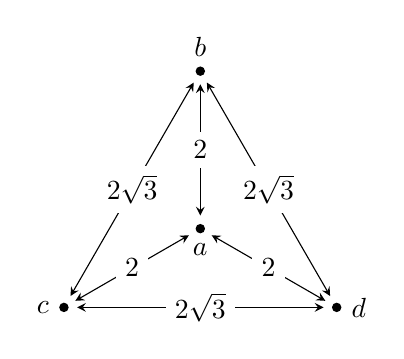
\begin{tikzpicture}[ >=stealth,
      dot/.style={circle,fill=black,inner sep=0,minimum size=1.2mm},
      len/.style={<->,shorten >=1mm,shorten <=1mm} ]
      % points
      \node[dot,label=below:{$a$}] (a) at (0,0) {};
      \node[dot,label=above:{$b$}] (b) at (90:2) {};
      \node[dot,label=left:{$c$}] (c) at (210:2) {};
      \node[dot,label=right:{$d$}] (d) at (330:2) {};

      % lengths
      \draw [len] (b) to (c);
      \draw [len] (c) to (d);
      \draw [len] (d) to (b);

      \draw [len] (a) to (b);
      \draw [len] (a) to (c);
      \draw [len] (a) to (d);      

      % labels
      \node[fill=white] at (270:1) {$2\sqrt{3}$};
      \node[fill=white] at (30:1) {$2\sqrt{3}$};
      \node[fill=white] at (150:1) {$2\sqrt{3}$};

      \node[fill=white] at (90:1) {$2$};
      \node[fill=white] at (210:1) {$2$};
      \node[fill=white] at (330:1) {$2$};
    \end{tikzpicture}
  \caption{A dataset in Euclidean space consisting of three points arranged in
  an equilateral triangle with another point at the centre.}
  \label{fig:points-in-plane}
\end{figure}

An all-squares optimal clustering, on the other hand, is not necessarily
linearly separable.  This can be shown by a simple example.  Consider a
dataset consisting of distinct points $a,b,c,d$ arranged in the Euclidean
plane as illustrated in Figure~\ref{fig:points-in-plane}.  There are $n$
copies of $a$ and one copy each of $b,c,d$.  The clustering $\clus =
\{\{(a,n)\},\{(b,1),(c,1),(d,1)\}\}$ has an all-squares cost of 72.  But if we
move one of $b,c,d$ into the first cluster, then we have a cost of $8n+24$
which is greater whenever $n>6$.  Similarly if we move two of $b,c,d$ into the
first cluster we get a cost of $16n+24$.  So whenever $n>6$ the all-squares
optimal clustering is $\clus$ and hence is not linearly separable.

% \subsection{Methods for finding optimal clusterings}
% \label{sec:meth-find-optim}

% In this paper we do not present any new methods for computing optimal
% clusterings, but we will briefly discuss existing methods and other
% possibilities here.  Optimal clustering is intuitively a hard problem.
% Centroid-distance clustering in Euclidean space was taken to be NP-complete
% for decades although this was proved only relatively
% recently\citep{aloise09exact}.  In the next section we will see that
% all-squares clustering is also NP-complete and for both problems we
% investigate the complexity for specific, very simple metric spaces.

% The consequence of the complexity of the problems is that heuristic algorithms
% for estimating optimal solutions are very prevalent; indeed, the $k$-means
% heuristic algorithm (also known as Lloyd's algorithm, although it was
% independently discovered by many different authors\citep{jain2010data}) for
% estimating the centroid-distance optimal $k$-clustering is probably the most
% well-known and widely-used clustering algorithm today.  Assuming that
% centroids are easy to compute, this algorithm is simple and, generally,
% quickly converges to a local optimum.  However, in the worst case, $k$-means
% requires exponentially many iterations in order to converge on a solution,
% even in the plane\citep{vattani2009exponential}.  There are many more
% heuristic methods for the problem; nine prominent methods are compared in
% \citep{brusco2007comparison}.

% Some algorithms for exactly solving the centroid-distance problem are known
% including methods using branch-and-bound \citep{brusco2006repetitive},
% branch-and-cut \citep{aloise09exact} and column generation
% \citep{merle1999interior}.  Some of these algorithms are able to exactly solve
% instances in the plane of around 2000 elements in reasonable time
% \citep{aloise09exact}.

% The all-squares problem, or more generally sum-of-cliques, has received less
% attention but there are, nonetheless, a number of algorithms described in the
% literature.  An exact algorithm using branch-and-bound
% \citep{klein1991optimal} can be used to solve problems with $n \leq 50, k \leq
% 5$ \citep{hansen1997mathprog}.  Cutting planes have also been applied with
% problems with $n \leq 158$ solved quickly
% \citep{hansen1997mathprog,palubeckis1997branch}.  In terms of heuristic
% approaches, there is an obvious iterative agglomerative technique that can be
% applied.  We have a simple randomised version that is showing some promise
% \citep{gk2012agglomerative}.

\section{Complexity issues}
\label{sec:complexity-issues}

We will now formally define the problems of finding an optimal clustering
according to either criteria and analyse the complexity of these problems.

\subsection{All-squares clustering}
\label{sec:all-squar-clust}

We state the all-squares problem formally as a decision problem:
\begin{problem}{All Squares Clustering (ASC)}
  \instance{A multiset of nodes $(\dset,\mu_{\dset})$, where $\dset =
    \{S_1,S_2,\dotsc,S_n\}$; a metric, $d$, which is defined for all elements
    in $\dset$; the number of clusters desired, $k \in \mathbb{Z}^+$ and a
    bound $B \in \mathbb{R}^+$.}  \question{Is there a $k$-clustering, $\clus
    = \{C_1,C_2,\dotsc,C_k\}$, such that
    \begin{equation*}
      cost_{as}(\clus)=
      \sum_{i=1}^{k} \sum_{x,y \in C_i} \mu_{C_i}(x)\mu_{C_i}(y)d^2(x,y)
      \leq B \quad \text{?}
    \end{equation*}}
\end{problem}

The problem is defined for multisets but, unless stated otherwise, the
NP-completeness proofs which follow are for sets, since this establishes the
result for multisets too.  When dealing with sets, the membership functions
are omitted since they are always equal to 1.

% so the cost function becomes simply
% \begin{equation*}
%   cost_{as}(\clus)=
%   \sum_{i=1}^{k} \sum_{x,y \in C_i} d^2(x,y).
% \end{equation*}

\subsubsection{Euclidean space}
\label{sec:euclidean-space}

An important special case of ASC is when the nodes are in Euclidean space and
we use the Euclidean metric $d_E$.  We call this special case Euclidean
all-squares clustering (EASC).

\begin{thm}
  EASC is NP-complete.
\end{thm}

\begin{proof}
  We observe that a guessed solution, $\clus_g$, can be checked in polynomial
  time by simply calculating $cost_{as}(\clus_g)$ and comparing the value to
  the bound.  Therefore $\text{EASC} \in \NP$.
  
  Now to show that EASC is NP-complete we construct a transformation from a
  known NP-complete problem to our problem.  The NP-complete problem we will
  use is the following \citep{gareyjohnson79}:
  \begin{problem}{Partition into Triangles (PT)}
    \instance{Graph $G = (V,E)$, with $|V| = 3q$ for some integer $q$.}
    \question{Can each of the vertices of $G$ be partitioned into $q$ disjoint
      sets $V_1,V_2,\dotsc,V_q$, each containing exactly $3$ vertices, such
      that for each $V_i = \{u_i,v_i,w_i\}, 1 \leq i \leq q$, all three of the
      edges $\{u_i,v_i\}, \{u_i,w_i\}$ and $\{v_i,w_i\}$ belong to $E$?}
  \end{problem}

  We transform an instance $I = G = (V,E)$ of PT, where $|V|=3p$, $V = \{v_0,
  \dotsc, v_{3p-1}\}$ and $|E|=m$ into an instance $f(I)$ of EASC: first we
  assign to $\dset$ a set of $n=3p$ points in $(3p+m)$-dimensional Euclidean
  space.  Each element $v_i \in V$ corresponds to a point where
  \begin{enumerate}
  \item the $i$th coordinate is $N = 2m$,
  \item all other coordinates $1 \leq i \leq 3p$ are 0,
  \item for $1 \leq j \leq m$, if $v_i$ is incident with $e_j \in E$ then the
    $(3p+j)$th coordinate is 1, otherwise it is 0.
  \end{enumerate}
  We then set $k$ to $p$ and $B$ to $8m-12p+12N^2p$.  It is easy to see that
  this transformation can be computed in polynomial time.

  \begin{lem}
    \label{lem:eq-dis}
    Let $\dset$ be a dataset with $|\dset| = n$ where the distance squared
    between each pair of distinct elements is $s$.  The sum-of-squares minimal
    $k$-clustering will contain clusters with cardinality of either
    $\left\lceil \frac{n}{k} \right\rceil$ or $\left\lfloor \frac{n}{k}
    \right\rfloor$ only.
  \end{lem}

  \begin{proof}
    The cost associated with a cluster, $C$, which contains $p$ elements is
    $p(p-1)s = (p^2-p)s$.  The extra cost of adding an element to $C$ is
    $((p+1)^2 - (p+1))s - (p^2-p)s = 2ps$, and the saving when removing an
    element is $(p^2 - p)s - ((p-1)^2 - (p-1))s = 2(p - 1)s$.

    We proceed by contradiction.  Assume that we have an optimal
    $k$-clustering, where $k \geq 2$ (the case where $k=1$ is trivial),
    including two clusters $C_i$ and $C_j$, where $|C_i| = p_i$, $|C_j| = p_j$
    and $p_i > p_j + 1$.  We move an element from $C_i$ to $C_j$; the
    difference in overall cost due to the move is $2p_js - 2p_is + 2s < 0$, so
    we have a saving.  Therefore our original clustering could not have been
    optimal.
  \end{proof}

  \begin{cor}
    \label{cor:extra-cost}
    Since $p_i \geq p_j + 2$, the difference in cost will be $(2p_j - 2p_i +
    2)s \leq 2s$.  Therefore, the cost of any suboptimal clustering will be at
    least $2s$ greater than the cost of the optimal clustering.
  \end{cor}

  In our reduction $\left\lceil \frac{n}{k} \right\rceil = \left\lfloor
    \frac{n}{k} \right\rfloor = 3$, so the optimal clustering when all nonzero
  distances are equal will be one where each cluster contains three elements.

  \begin{lem}
    \label{lem:euclidean-iff}
    $I$ is a YES instance of PT if and only if $f(I)$ is a YES instance of EASC.
  \end{lem}

  \begin{proof}
    If $I \in Y_{\text{PT}}$ then we can construct a clustering by letting
    each cluster correspond to one of the triangles in the partition of $G$.
    Let $w,x,y$ be the vertices of such a triangle, and therefore a cluster.
    The distance squared between a pair of these points is $d^2(w,x) =
    2N^2+\deg(w)+\deg(x)-2$; the $2N^2$ comes from the coordinates governed by
    rules 1 and 2 in the transformation and the $\deg(w) + \deg(x) - 2$ comes
    from the coordinates governed by rule 3.  The overall cost of the
    clustering is therefore $2(2\deg(w)+2\deg(x)+2\deg(y)+6N^2-6)$.  Hence,
    the set of $p$ triangles has cost
    \begin{equation}
      \label{eq:tri-cost}
      4\sum_{v \in V} \deg(v) + 12N^2p - 12p = 8m + 12N^2p - 12p = B,
    \end{equation}
    so $f(I) \in Y_{\text{EASC}}$.

    If $f(I) \in Y_{\text{EASC}}$ then we have a $k$-clustering which fits the
    bound.  The distance between each pair of distinct points in the dataset
    is at least $2N^2$.  Assume that the distances are all exactly $2N^2$: due
    to Lemma~\ref{lem:eq-dis}, the optimal clustering in this case is one
    where each cluster contains 3 elements, and this clustering has an overall
    cost of $12N^2p$.  Due to Corollary~\ref{cor:extra-cost}, any suboptimal
    clustering would have an overall cost of at least $(12p+4)N^2$ and, since
    $N^2=4m^2$, will not meet the bound.  Clearly, if one of these suboptimal
    clusterings contained distances greater than $2N^2$ in the sum their
    overall cost would be greater still.  Therefore, each cluster must contain
    exactly 3 elements.

    As shown in equation~\eqref{eq:tri-cost}, the cost of a clustering where
    each cluster corresponds to a triangle in $G$ equals the bound.  If some
    cluster does not correspond to a triangle, then its cost is increased, and
    therefore the overall cost of the clustering will be greater than the
    bound.  So each cluster must be a triangle, so $I \in Y_{\text{PT}}$.
  \end{proof}
  Hence, due to Lemma~\ref{lem:euclidean-iff}, the theorem is established.
\end{proof}

\subsubsection{$p$-valued metric}
\label{sec:p-valued-metric}

\begin{dfn}
  A \textbf{$p$-valued metric} is a metric where the cardinality of the
  codomain is equal to some positive integer $p$.
\end{dfn}

\begin{thm}
  \label{thm:np-complete-3-val}
  ASC is NP-complete even with a 3-valued metric.
\end{thm}

\begin{proof}
  We observe that a guessed solution can be checked in polynomial time,
  therefore $\text{ASC} \in \NP$.

  Now we choose again to construct a transformation from \textsc{Partition
    into Triangles} (PT).  An instance $I$ of PT is transformed into an
  instance $f(I)$ of ASC as follows: first we construct a 3-valued metric
  space by setting $\dset$ to $V$ and defining a function $d \colon \dset
  \times \dset \to \{0,\alpha,\beta\}$ where $0 > \alpha > \beta$ by
  \begin{equation*}
    d(u,v) = \begin{cases}
      0 & \text{if $u=v$,}\\
      \alpha & \text{if there exists an edge in $G$ between $u$ and $v$,}\\
      \beta & \text{otherwise.}
    \end{cases}
  \end{equation*}

  \begin{lem}
    \label{lem:3-val-met}
    $(\dset,d)$ is a metric space.
  \end{lem}
  
  \begin{proof}
    We show that $d$ satisfies each condition required for a metric for all
    $u,v,w \in \dset$:
    \begin{enumerate}
    \item $d(u,v)=0$ if and only if $u=v$ by definition,
    \item $d(u,v)=d(v,u)$ by definition,
    \item $d(u,v)+d(v,w) \geq d(u,w)$ (triangle inequality)\\
      If $u=w$ then this is trivially true.\\
      If $d(u,w)=\alpha$ then $u \neq w$ so either $u \neq v$ or $v \neq w$ or
      both.\\
      If $d(u,w)=\beta$ then $u \neq w$ and there is no edge between $u$ and
      $w$, we then have two cases: either both $u \neq v$ and $v \neq w$ which
      satisfies the inequality, or one of $u=v$ or $v=w$, but we know there is
      no edge between $u$ and $w$ so therefore there is no edge between $v$
      and $w$ or $v$ and $u$ respectively, so the inequality is satisfied.
    \end{enumerate}
  \end{proof}

  We then set $B$ to $6q\alpha$ and $k$ to $q$ to complete the transformation.
  It is easy to see that this transformation can be computed in polynomial
  time.

  \begin{lem}
    \label{lem:3-val-iff}
    $I$ is a YES instance of PT if and only if $f(I)$ is a YES instance of ASC.
  \end{lem}

  \begin{proof}
    If $I \in Y_{\text{PT}}$ then observe that we can construct a clustering,
    $\clus$, by assigning to each cluster $C_i$ the set $V_i$.  Since each
    $V_i$ has an edge between each pair of vertices, the cost of each cluster
    $C_i$ is $6\alpha$, and therefore the cost of $\clus$ is $6q\alpha$.  So
    therefore $f(I) \in Y_{\text{ASC}}$.

    If $I \in N_{\text{PT}}$ then we cannot have a clustering where all
    clusters have cardinality $3$ as this will contain at least one distance
    greater than $\alpha$ and therefore not meet the bound.  We must consider
    clusterings where all within cluster distances are equal to $\alpha$, but
    due to Lemma~\ref{lem:eq-dis}, any such clustering with clusters of
    different sizes always has a higher cost so they also cannot meet the
    bound.  Therefore $f(I) \in N_{\text{ASC}}$.
  \end{proof}

  Hence, due to Lemmata~\ref{lem:3-val-met} and \ref{lem:3-val-iff}, the
  theorem is established.

\end{proof}

\begin{thm}
  \label{thm:asc-np-complete-n-val}
  For all $n \geq 3$ there exists a metric such that ASC is hard, therefore
  ASC is NP-complete with an n-valued metric when $n \geq 3$.
\end{thm}

\begin{proof}
  We proceed by induction.  Theorem~\ref{thm:np-complete-3-val} establishes
  the base case, so we now assume that the problem is NP-complete with an
  $n$-valued metric and show that it is NP-complete with an $(n+1)$-valued
  metric.

  We transform an instance, $I$, of the $n$-valued problem into an instance,
  $f(I)$ of the $(n+1)$-valued problem.  Let $\dset^*$, $d^*$, $k^*$ and $B^*$
  be the dataset, metric, number of clusters and bound of $f(I)$,
  respectively.  We set $\dset^*$ to $\dset \cup \{a\}$, $k^*$ to $k+1$ and
  $B^*$ to $B$.  We define a function $d^* \colon \dset \times \dset$ by
  \begin{equation*}
    d^*(x,y) =
    \begin{cases}
      0 & \text{if $x=y$,}\\
      s & \text{if $x=a$ or $y=a$,}\\
      d(x,y) & \text{otherwise,}
    \end{cases}
  \end{equation*}
  where $s = \sum_{p,q \in \dset} d^2(p,q)$.  Notice that the distance between
  $a$ and each element in $\dset$ is the complete sum of all distances squared
  in $\dset$.  It is easy to see that this transformation can be computed in
  polynomial time.

  \begin{lem}
    \label{lem-asc-n-val-iff}
    $I$ is a YES instance of $n$-valued ASC if and only if $f(I)$ is a YES
    instance of $(n+1)$-valued ASC.
  \end{lem}
  \begin{proof}
    If $I \in Y_{ASC}$ then there is some clustering $\clus =
    \{C_1,C_2,\dotsc,C_k\}$ of $\dset$ with a cost less than or equal to $B$.
    We can construct a similar clustering of $\dset^*$ : $\clus^* = \clus \cup
    \{\{a\}\}$.  The extra cluster will not contribute to the cost, so the
    cost of $\clus^*$ is also less than or equal to $B$, so $f(I) \in
    Y_{ASC}$.

    If $f(I) \in Y_{ASC}$ then there is some clustering, $\clus^* =
    \{C^*_1,C^*_2,\dotsc, C^*_{k^*}\}$, with cost less than or equal to $B$.
    Let $C^*_l$ be the cluster which contains the element $a$.  If some other
    elements belong to this cluster then we can move them into any other
    cluster: each element we move makes a saving of at least $s^2$ but the
    final overall cost of the cluster we move them to can be at worst $s$, so
    clearly this will result in a saving.  Now, $C_l$ contains only $a$ so
    does not contribute to the overall cost, so $\clus^* \setminus C^*_l$ has
    an overall cost less than or equal to $B$ and therefore $I \in Y_{ASC}$.
  \end{proof}

  Hence, due to Lemma~\ref{lem-asc-n-val-iff}, the theorem is established.
\end{proof}

If our dataset is a set and the metric is 2-valued then the problem is
solvable in polynomial time due to Lemma~\ref{lem:eq-dis}.  We need only solve
the equation
\begin{equation*}
  x \left\lceil\frac{n}{k}\right\rceil
  + (k-x) \left\lfloor\frac{n}{k}\right\rfloor = n
\end{equation*}
for $x$ and an optimal clustering is then $x = n-k\lfloor\frac{n}{k}\rfloor$
clusters of $\lceil\frac{n}{k}\rceil$ elements and $k-x$ clusters of
$\lfloor\frac{n}{k}\rfloor$ elements.  For the decision version we would then
simply calculate the cost of the clustering to see if it is less than the
bound.  We conclude with:
\begin{thm}
  When the dataset is a set with a 2-valued metric, an optimal clustering can
  be found in polynomial time.
\end{thm}

However, if the dataset is a multiset this is not the case; the problem
becomes NP-complete.
\begin{thm}
  \label{thm:2-met-multiset-np-complete}
  When the dataset is a multiset with a 2-valued metric, ASC is an NP-complete
  problem.
\end{thm}

\begin{proof}
  We construct a transformation from the NP-complete problem
  \citep{gareyjohnson79}:
  \begin{problem}{Minimum Sum of Squares (MSS)}
    \instance{Finite set $A$, a size $s(a) \in \mathbb{Z}^+$ for each $a \in
      A$, positive integers $K \leq |A|$ and $J$.}
    \question{Can $A$ be partitioned into $K$ disjoint sets
      $A_1,A_2,\dotsc,A_k$ such that
      \begin{equation*}
        \sum_{i=1}^{K}\left(\sum_{a \in A_i} s(a)\right)^2 \leq J \quad ?
      \end{equation*}
    }
  \end{problem}
  We construct our dataset by setting $\dset$ to $A$ and $\mu_{\dset}$ to $s$
  and we set $k$ to $K$.  We define a metric $d$ for all $u,v \in \dset$ as
  \begin{equation*}
    d(u,v) =
    \begin{cases}
      0 & \text{if $u=v$,}\\
      1 & \text{otherwise.}
    \end{cases}
  \end{equation*}

  To find the value for $B$, consider an optimal multiset clustering
  $\clus=\{C_1,C_2,\dotsc,C_k\}$ which is consistent, so
  $\mu_{C_i}(x)=\mu_{\dset}(x)$ for all $x \in \dset$ and $1 \leq i \leq k$.
  The cost of a single cluster, $C_i$, is
  \begin{equation*}
    \sum_{x,y \in C_i} \mu_{\dset}(x)\mu_{\dset}(y)
    = \left(\sum_{x \in C_i} \mu_{\dset}(x)\right)^2
    - \sum_{x \in C_i} (\mu_{\dset}(x))^2,
  \end{equation*}
  so the total cost of $\clus$ is
  \begin{equation}
    \label{eq:clus-tot}
    \sum_{i=1}^{k}\left(\sum_{x \in C_i} \mu_{\dset}(x)\right)^2
    - \sum_{i=1}^{k}\sum_{x \in C_i} (\mu_{\dset}(x))^2.
  \end{equation}
  The second term is a constant and is equivalent to
  \begin{equation*}
    \Gamma = \sum_{x \in \dset} (\mu_{\dset}(x))^2.
  \end{equation*}
  We set $B$ to $J-\Gamma$ and the transformation is complete.  It is now easy
  to see that the cost of the optimal clustering, $\clus$, will meet the
  bound, $B$, if and only if the first term in expression~\eqref{eq:clus-tot}
  is less than or equal to $J$.  So $I \in Y_{\text{MSS}}$ if and only if
  $f(I) \in Y_{\text{ASC}}$ and the theorem is established.
\end{proof}

\subsection{Centroid-distance clustering}
\label{sec:centr-dist-clust}

Again, we state the problem formally as a decision problem:
\begin{problem}{Centroid-Distance Clustering (CDC)}
  \instance{A metric space $(M,d)$, a set of nodes $\dset \subseteq M$, the
    number of clusters desired, $k \in \mathbb{Z}^+$, and a bound, $B \in
    \mathbb{R}^+$.}
  \question{Is there a $k$-clustering, $\clus = \{C_1,C_2,\dotsc,C_k\}$ such
    that
    \begin{equation*}
      cost_{cd}(\clus)
      = \sum_{i=1}^{k} \sum_{x \in C_i} \mu_i(x) d^2(x,c_i) \leq B,
    \end{equation*}
    where $c_i \in M$ is the centroid of cluster $C_i$?
  }
\end{problem}
Again, the problem is defined for multisets, but the following proof is for
sets so the membership function has been omitted.

\begin{thm}
  \label{thm:CDC-NP}
  CDC is NP-complete.
\end{thm}

\begin{proof}
  We observe that a guessed solution, $\clus_g$, can be checked in polynomial
  time, therefore $\text{CDC} \in \NP$.

  To show that CDC is NP-complete we will construct a transformation from a
  known NP-complete problem to our problem.  The problem we will use is the
  following \cite{gareyjohnson79}:
  \begin{problem}{Dominating Set (DS)}
    \instance{A graph $G=(V,E)$ and a positive integer $K \leq |V|$.}
    \question{Is there a dominating set of size $K$ or less for $G$ or, in
      other words, a subset $V' \subseteq V$ with $|V'| \leq K$ such that for
      all $u \in V \setminus V'$ there is a $v \in V'$ for which $\{u,v\} \in
      E$?  }
  \end{problem}

  We transform an instance $I$ of DS into an instance $f(I)$ of CDC.  Fist we
  construct a 3-valued metric space by setting $M = \dset$ to $V$ and define a
  function $d \colon M \times M \to \rr$ by
  \begin{equation*}
    d(u,v) = \begin{cases}
      0 & \text{if $u=v$,}\\
      1 & \text{if there exists an edge in $G$ between $u$ and $v$,}\\
      2 & \text{otherwise.}
    \end{cases}
  \end{equation*}

  This is a metric space by Lemma~\ref{lem:3-val-met}. We then set $k$ to $K$
  and $B$ to $n-k$.

  \begin{lem}
    \label{lem:iff}
    $I$ is a YES instance of DS if and only if $f(I)$ is a YES instance of CDC.
  \end{lem}

  \begin{proof}
    If $I \in Y_{DS}$ then $|V'| \leq K = k$.  We can construct a
    $k$-clustering by first picking $k-|V'|$ arbitrary elements from $V
    \setminus V'$ and adding each of these to separate clusters.  These are
    final clusters and will not contribute to the overall cost.  We then add
    one element of the dominating set each to the remaining $|V'|$ clusters.
    These elements are the tentative centroids of the clusters.  So far we
    still have an overall cost of zero.  The remaining $n-k$ elements are
    added one by one to any cluster where they share an edge with the
    tentative centroid.  Thus, each of these $n-k$ elements contributes to the
    cost by 1.  If one of the final centroids of these constructed clusters
    turns out to be different to the tentative centroids, this can only
    decrease the cost of that cluster, by the definition of a centroid.
    Therefore the overall cost is less than or equal to $B = n-k$, so $f(I)
    \in Y_{CDC}$.

    \begin{figure}
      \centering
      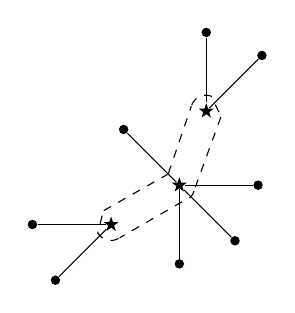
\begin{tikzpicture}[
        node/.style={circle,fill=black,inner sep=0,minimum size=1.2mm},
        cent/.style={star,star point height=0.6mm,fill=black,inner sep=0,minimum size=2mm},
        edge/.style={-},
        outl/.style={dashed},
        help/.style={inner sep=0,minimum size=0mm}]

        % dominating set nodes (centroids)
        \node[cent] (1) at (0,0) {};
        \node[cent] (2) at (70:1) {};
        \node[cent] (3) at (210:1) {};

        % other nodes
        \begin{scope}
          \node[node] (11) at (0:1) {};
          \node[node] (12) at (135:1) {};
          \node[node] (13) at (270:1) {};
          \node[node] (14) at (315:1) {};
          % helpers
          \node[help] (1h1) at (135:0.2) {};
          \node[help] (1h2) at (-20:0.2) {};
          \node[help] (1h3) at (300:0.2) {};
        \end{scope}
        
        \begin{scope}[shift={(70:1)}]
          \node[node] (21) at (45:1) {};
          \node[node] (22) at (90:1) {};
          % helpers
          \node[help] (2h1) at (-20:0.2) {};
          \node[help] (2h2) at (70:0.2) {};
          \node[help] (2h3) at (160:0.2) {};
        \end{scope}

        \begin{scope}[shift={(210:1)}]
          \node[node] (31) at (225:1) {};
          \node[node] (32) at (180:1) {};
          % helpers
          \node[help] (3h1) at (120:0.2) {};
          \node[help] (3h2) at (210:0.2) {};
          \node[help] (3h3) at (300:0.2) {};
        \end{scope}

        % edges
        \foreach \n in {11,12,13,14} {
          \draw [edge] (1) to (\n);
        }

        \foreach \n in {21,22} {
          \draw [edge] (2) to (\n);
        }

        \foreach \n in {31,32} {
          \draw [edge] (3) to (\n);
        }

        % dominating set outline
        \draw[outl] (1h1) -- (2h3) to [bend left=45] (2h2) to (2h1) -- (1h2)
        to [bend left=25] (1h3) -- (3h3) to [bend left=45] (3h2) to (3h1) -- (1h1);
      \end{tikzpicture}
      \caption{Each of the $k$ clusters correspond to star graphs with the
        centroid at the centre, so there is a dominating set of size $k$ as
        outlined.}
      \label{fig:domset}
    \end{figure}

    If $f(I) \in Y_{\text{CDC}}$ then we have an overall cost of less than or
    equal to $n-k$.  Since $\dset = M$, each cluster must contain an element
    equal to the centroid of that cluster, so there are exactly $k$ elements
    which do not contribute to the overall cost.  Each of the $n-k$ remaining
    elements must contribute to the cost by at least $1$, so therefore must
    contribute by exactly $1$ giving an overall cost of exactly $n-k$.  Each
    cluster therefore corresponds to a star in $G$, as illustrated in
    Figure~\ref{fig:domset}, so $I \in Y_{\text{DS}}$.
  \end{proof}

  Hence, due to Lemmata~\ref{lem:3-val-met} and \ref{lem:iff}, the theorem is
  established.
\end{proof}

Theorem~\ref{thm:CDC-NP} has already been established using Euclidean space.
In fact, the problem has been shown to be NP-hard for both $k=2$ in general
Euclidean space \citep{aloise09} and for general $k$ in only 2 dimensions
\citep{mahajan09}.  If both $k$ and $d$, the number of dimensions, are fixed,
the problem is exactly solvable in $O(n^{dk+1} \log n)$
time\citep{inaba94weightedvoronoi}.

Our proof establishes the following new result:
\begin{cor}
  Even if the metric, $d$, is a 3-valued metric, centroid-distance clustering
  remains an NP-complete problem.
\end{cor}

\begin{thm}
  \label{thm:cdc-np-complete-n-val}
  For all $n \geq 3$ there exists a metric such that CDC is hard, therefore
  CDC is NP-complete with an n-valued metric when $n \geq 3$.
\end{thm}

\begin{proof}
  We proceed by induction.  Theorem~\ref{thm:CDC-NP} establishes the base
  case, so we now assume that the problem is NP-complete with an $n$-valued
  metric and show that it is NP-complete with an $(n+1)$-valued metric.

  We use the same transformation as used for the proof of
  Theorem~\ref{thm:asc-np-complete-n-val}.

  \begin{lem}
    \label{lem-cdc-n-val-iff}
    $I$ is a YES instance of $n$-valued CDC if and only if $f(I)$ is a YES
    instance of $(n+1)$-valued CDC.
  \end{lem}

  \begin{proof}
    If $I \in Y_{CDC}$ then there is some clustering $\clus =
    \{C_1,C_2,\dotsc,C_k\}$ of $\dset$ with a cost less than or equal to $B$.
    We can construct a similar clustering of $\dset^*$: $\clus^* = \clus \cup
    \{\{a\}\}$.  The extra cluster will not contribute to the cost, so the
    cost of $\clus^*$ is also less than or equal to $B$, so $f(I) \in
    Y_{CDC}$.

    If $f(I) \in Y_{CDC}$ then there is some clustering $\clus^* =
    \{C^*_1,C^*_2,\dotsc,C^*_{k^*}\}$ which has cost less than or equal to
    $B$.  Let $C^*_l$ be the cluster which contains element $a$.  If other
    elements belong to this cluster then the cluster will have cost greater
    than or equal to $s^2$.  We can move all other elements to any other
    cluster, say $C^*_p$, which will reduce the cost of $C^*_l$ to 0, but the
    cost of $C^*_p$ must be less than $s$, so we have an overall saving.  Now
    $C^*_l$ does not contribute to the overall cost, so $\clus^* \setminus
    C^*_l$ has an overall cost less than or equal to $B$ and therefore $I \in
    Y_{CDC}$.
  \end{proof}
  Hence, due to Lemma~\ref{lem-cdc-n-val-iff}, the theorem is established.
\end{proof}

However, when the metric is 2-valued, the problem is solvable in polynomial
time, even in the multiset case.  To see this, let our metric be
\begin{equation*}
  d(u,v) =
  \begin{cases}
    0 & \text{if $u=v$,}\\
    s & \text{otherwise.}
  \end{cases}
\end{equation*}

The overall cost of a clustering will be
\begin{equation*}
  \sum_{i=1}^{k} \sum_{\{x \in C_i,x \neq c_i\}} \mu_{i}(x)s^2
\end{equation*}
or, equivalently,
\begin{equation*}
  \sum_{x \in \dset} \mu_{\dset}(x)s^2 - \sum_{i=1}^{k} \mu_{i}(c_i)s^2.
\end{equation*}
The first term is a constant, so the problem is to simply maximise the second
term.  This can be done by ordering the elements of $\dset$ by their
membership count in descending order and selecting the first $k$ elements.  We
move all copies of each of the selected elements to their own cluster; these
will become the centroids.  The remaining elements may then be moved to an
arbitrary cluster as they will all contribute to the cost by $s$ each in any
case.

\section{The assignment metric}
\label{sec:metr-comp-clust}

There are many existing methods for comparing clusterings.  Many do not
provide us with, or do not have established, bounds so are not very useful for
our purposes.  We will look at two metrics which have upper bounds: the
Variation of Information (VI) (see Section~\ref{sec:inform-theor}) and our
assignment metric which we present here.  The assignment metric is based on
set matching like those discussed in Section~\ref{sec:set-matching}, but
allows any metric to be used for comparing the matched sets.

Let $\mathcal{P}_k$ be the set of all possible $k$-clusterings of $\dset$.
We define the assignment metric as a function $\Delta \colon \mathcal{P}_k
\!\times \mathcal{P}_k \to \mathbb{R}$ where
\begin{equation*}
  \Delta(\clus_1, \clus_2) = \min_{\sigma \in S_k} \sum_{i=1}^{k}
  \delta(C_{1i}, C_{2\sigma(i)})
\end{equation*}
for some $\delta \colon (2^{\dset} \setminus \emptyset) \times (2^{\dset}
\setminus \emptyset) \to \mathbb{R}$ and where $S_k$ is the set of all
possible functions $\sigma \colon \{1, \dotsc, k\} \to \{1, \dotsc, k\}$.

\begin{thm}
  The measure $\Delta$ is a metric on $\mathcal{P}_k$ whenever $\delta$ is a
  metric on $(2^{\dset} \setminus \emptyset)$.
\end{thm}

\begin{proof}
  We show that $\Delta$ satisfies all conditions required for a metric:
  \begin{enumerate}
  \item $\Delta(\clus_1, \clus_2) \geq 0$ trivially since
    $\delta(C_{1i}, C_{2j}) \geq 0$ for all $1 \leq i,j \leq k$ since
    $\delta$ is itself a metric,
  \item If $\clus_1 = \clus_2$ then there exists some $\sigma$ for which
    $C_{1i} = C_{2\sigma(i)}$ and therefore $\delta(C_{1i},
    C_{2\sigma(i)}) = 0$ for all $1 \leq i \leq k$, so $\Delta(\clus_1,
    \clus_2) = 0$.

    If $\Delta(\clus_1, \clus_2) = 0$ then $\delta(C_{1i},
    C_{2\sigma(i)}) = 0$ and therefore $C_{1i} = C_{2\sigma(i)}$ for
    some $\sigma$ and all $1 \leq i \leq k$, so $\clus_1 = \clus_2$,
  \item $\Delta(\clus_1, \clus_2) = \Delta(\clus_2, \clus_1)$
    trivially since $\delta(C_{1i}, C_{2j}) = \delta(C_{2j}, C_{1i})$
    for all $1 \leq i,j \leq k$,
  \item Let $\Delta(\clus_1, \clus_2) = \sum_{i=1}^{k} \delta(C_{1i},
    C_{2\sigma(i)})$ for
    some $\sigma \in S_k$\\
    and $\Delta(\clus_2, \clus_3) = \sum_{i=1}^{k} \delta(C_{2i},
    C_{\uptau(i)})$ for some $\uptau \in S_k$.
    
    Then,
    \vspace{-1em}
    \begin{align*}
      \Delta(\clus_1, \clus_2) + \Delta(\clus_2, \clus_3) &=
      \sum_{i=1}^{k} \delta(C_{1i},
      C_{2\sigma(i)}) + \delta(C_{2\sigma(i)}, C_{3\uptau(\sigma(i))})\\
      &\geq \sum_{i=1}^{k} \delta(C_{1i},
      C_{3\uptau(\sigma(i))})\quad\text{(due to
        triangle inequality of $\delta$)}\\
      &\geq \min_{\sigma \in S_k} \sum_{i=1}^{k} \delta(C_{1i}, C_{3\sigma(i)})\\
      &= \Delta(\clus_1, \clus_3).
    \end{align*}
  \end{enumerate}
\end{proof}

Possible choices for the $\delta$ metric are the cardinality of the symmetric
difference, $\delta(A,B) = |A \symdif B|$, and the normalised symmetric
difference, also known as the Jaccard distance, $\delta(A,B) = \frac{|A
  \symdif B|}{|A \cup B|}$.  These are well known metrics with the former
being used often in the literature for comparing sets, for example in
\cite{reynolds2006clustering}.  These two metrics extend naturally to
multisets; the multiset version of symmetric difference is
$\delta((A,\mu_A),(B,\mu_B)) = \sum_{x,y \in A \cup B} |\mu_A(x)-\mu_B(y)|$.

Calculating $\Delta$ amounts to calculating the minimum cost matching between
the clusters.  There are $k!$ possible matchings, but the minimum can be found
in $O(k^3)$ time using the Hungarian algorithm \cite{kuhn1955hungarian}.
Since $k! < k^3$ when $k < 6$, it may be more efficient to simply enumerate
all solutions when $k$ is small.

Clusterings with different $k$ can be compared by the addition of the
pseudometric $||\clus_1|-|\clus_2||$ (ie. the absolute difference between the
set cardinalities).  Let $\mathcal{P}$ be the set of all partitions of
$\dset$.  The assignment metric then becomes a function $\Delta \colon
\mathcal{P} \times \mathcal{P} \to \mathbb{R}$ defined as
\begin{equation*}
  \Delta(\clus_1, \clus_2)
  = \min_{\sigma \in S_k} \sum_{i=1}^{k} \delta(C_{1i},C_{2\sigma(i)})
  + \lambda ||\clus_1|-|\clus_2||,
\end{equation*}
where $k = \min(|C_1|,|C_2|)$, $\delta \colon (2^{\dset}\setminus \emptyset)
\times (2^{\dset}\setminus \emptyset) \to \mathbb{R}$ and $\lambda$ is a
positive real number.

This is most sensible when the metric $\delta$ is bounded or normalised and
$\lambda$ is greater than or equal to the upper bound on $\delta$.
Calculation of the metric using the Hungarian algorithm can then be performed
by a simple modification, namely by setting the cost of matching a set to
nothing as $\lambda$ and finding the minimum matching in the same way.

Using a bounded metric does not limit our choice since any metric can be
bounded.  One general formula for bounding a metric by $[0,1]$ is
\begin{equation}
  \label{eq:met-bound}
  \delta_b (A,B) = \frac{\delta(A,B)}{1+\delta(A,B)}.
\end{equation}
Alternatively, it may be possible to normalise the metric, as with the
normalised symmetric difference metric.

This version of the assignment metric is bounded by $\lambda \cdot
\max(|\clus_1|,|\clus_2|)$, and this bound is approached arbitrarily closely
by $\clus_1 = \{\{1,2,\dotsc,n\}\}, \clus_2 = \{\{1\},\{2\},\dotsc,\{n\}\}$ in
the limit of large $n$ for any metric $\delta$.  Tighter bounds may exist for
specific choices of $\delta$ and fixed $k$ (we prove one in
Section~\ref{sec:upper-bound}).

In Section~\ref{sec:asgn-met-fuzzy-partitions} we show how the assignment
metric can be used to compare fuzzy partitions and in
Section~\ref{sec:lifting-metric-space} we discuss the use of metrics which are
aware of the underlying metric space of a clustering.  In
Section~\ref{sec:worst-case-perf} we use the symmetric difference to prove a
worst case result for our two clustering criteria.

\subsection{Comparing fuzzy partitions}
\label{sec:asgn-met-fuzzy-partitions}

The assignment metric extends easily to fuzzy partitions.  All we need is a
metric on fuzzy sets.  Here we present such a metric which is analogous to the
symmetric difference.

Let $\mathcal{F}_f$ be the set of all fuzzy sets and $\mathcal{F}_c \subset
\mathcal{F}_f$ the set of all crisp sets.  Note that a crisp set is a special
case of a fuzzy set where
\begin{equation*}
  \mu_A(x) =
  \begin{cases}
    1 & \text{if $x \in A$}\\
    0 & \text{if $x \notin A$}
  \end{cases}
\end{equation*}
for all $A \in \mathcal{F}_c$.

We now define a function $\delta_f \colon \mathcal{F}_f \times \mathcal{F}_f
\to \mathbb{R}$ by
\begin{equation*}
  \delta_f(A,B) = \sum_{x \in \mathcal{R}} |\mu(x,A) - \mu(x,B)|.
\end{equation*}

\begin{thm}
  The measure $\delta_f$ is equivalent to the symmetric difference
  $\delta(A,B) = |A \symdif B|$ for all $A,B \in \mathcal{F}_c$.
\end{thm}

\begin{proof}
  For each $x \in \mathcal{R}$:
  \begin{enumerate}
  \item If $x \notin A$ and $x \notin B$ then $\mu(x,A) = \mu(x,B) = 0$ and
    therefore this does not contribute to the sum in $\delta_f(A,B)$,
  \item if $x \in A$ and $x \notin B$ then $\mu(x,A) = 1$ and $\mu(x,B) = 0$
    so $|\mu(x,A) - \mu(x,B)| = |1 - 0| = 1$,
  \item similarly, if $x \notin A$ and $x \in B$ then $|\mu(x,A) - \mu(x,B)|
    = |0 - 1| = 1$,
  \item if $x \in A$ and $x \in B$ then $|\mu(x,A) - \mu(x,B)| = |1 - 1| = 0$
    and therefore also does not contribute to the sum.
  \end{enumerate}
\end{proof}

For fuzzy sets this measure does correspond to $|A \symdif B| = |A \cup B|
- |A \cap B|$ since
\begin{align*}
  \mu(x, A \cup B) &= \max(\mu(x,A), \mu(x,B))\\
  \mu(x, A \cap B) &= \min(\mu(x,A), \mu(x,B))
\end{align*}
so the cardinality $|A \cup B| - |A \cap B|$ is
\begin{align*}
  &\sum_{x \in \mathcal{R}} \big(\max(\mu(x,A),\mu(x,B)) - \min(\mu(x,A),\mu(x,B))\big)\\
  &= \sum_{x \in \mathcal{R}} |\mu(x,A) - \mu(x,B)|
\end{align*}

\begin{thm}
  $(\mathcal{F}_f, \delta_f)$ is a metric space.
\end{thm}

\begin{proof}~
  
  \begin{enumerate}
  \item $\delta_f(A,B) = 0 \iff A=B$:
    \begin{align*}
      \delta_f(A,B) = 0 &\iff \mu(x,A) = \mu(x,B) \quad \forall x \in
      \mathcal{R}\\
      &\iff A = B,
    \end{align*}
  \item $\delta_f(A,B) = \delta_f(B,A)$ by definition,
  \item $\delta_f(A,B)+\delta_f(B,C) \geq \delta_f(A,C)$ (the triangle
    inequality):
    \begin{align*}
      \delta_f(A,B) + \delta_f(B,C)
      &= \sum_{x \in \mathcal{R}} |\mu(x,A) - \mu(x,B)|
      + \sum_{x \in \mathcal{R}} |\mu(x,B) - \mu(x,C)|\\
      &= \sum_{x \in \mathcal{R}} \big(|\mu(x,A)-\mu(x,B)|
      + |\mu(x,B)-\mu(x,C)|\big)\\
      &\geq \sum_{x \in \mathcal{R}} |\mu(x,A) - \mu(x,C)|\\
      &= \delta_f(A,C)
    \end{align*}
  \end{enumerate}
\end{proof}

There is also a corresponding normalised version of this metric for use with
the second version of the assignment metric:
  \begin{equation*}
    \delta_{f_n}(A,B) = \frac{|A \symdif B|}{|A \cup B|}.
  \end{equation*}

\subsection{Lifting the underlying metric space}
\label{sec:lifting-metric-space}

\begin{figure}
  \centering
  \begin{subfigure}[b]{0.3\textwidth}
    \begin{tikzpicture}
      \begin{axis}[xmin=0,xmax=10,ymin=0,ymax=10,width=1.2\textwidth,tick label style={font=\tiny}]
        \addplot+[only marks,color=blue,mark=o] table {
          2.0 2.0
          1.0 2.0
          2.0 1.0
          0.9 2.3
          2.1 0.7
          1.4 1.3
          2.6 2.8
          2.3 1.2
          3.6 2.1
          4.6 2.4
          3.6 2.5
          3.4 1.2
        };
        \addplot+[only marks,color=red,mark=x] table {
          8.0 2.0
          6.2 2.6
          8.8 3.9
          7.6 2.4
          7.2 3.2
          5.6 2.0
          8.7 2.4
          8.9 1.5
          7.0 2.0
          6.5 1.7
          7.3 1.6
          5.8 1.5
        };
        \addplot+[only marks,color=brown,mark=triangle] table {
          5.0 8.0
          5.5 8.6
          5.7 7.2
          5.2 6.2
          6.8 8.2
          5.2 6.7
          3.8 9.2
          3.7 8.2
          4.3 6.2
          4.9 6.7
          5.0 9.0
          4.5 8.6
        };
      \end{axis}
    \end{tikzpicture}
    \caption{Clustering $\clus_1$.}
    \label{fig:clus1}
  \end{subfigure}
  \begin{subfigure}[b]{0.3\textwidth}
    \begin{tikzpicture}
      \begin{axis}[xmin=0,xmax=10,ymin=0,ymax=10,width=1.2\textwidth,tick label style={font=\tiny}]
        \addplot+[only marks,color=blue,mark=o] table {
          2.0 2.0
          1.0 2.0
          2.0 1.0
          0.9 2.3
          2.1 0.7
          1.4 1.3
          2.6 2.8
          2.3 1.2
          3.6 2.1
          4.6 2.4
          3.6 2.5
          3.4 1.2
          5.2 6.2
          4.3 6.2
          4.9 6.7
          5.2 6.7        
        };
        \addplot+[only marks,color=red,mark=x] table {
          8.0 2.0
          6.2 2.6
          8.8 3.9
          7.6 2.4
          7.2 3.2
          5.6 2.0
          8.7 2.4
          8.9 1.5
          7.0 2.0
          6.5 1.7
          7.3 1.6
          5.8 1.5
        };
        \addplot+[only marks,color=brown,mark=triangle] table {
          5.0 8.0
          5.5 8.6
          5.7 7.2
          6.8 8.2
          3.8 9.2
          3.7 8.2
          5.0 9.0
          4.5 8.6
        };
      \end{axis}
    \end{tikzpicture}
    \caption{Clustering $\clus_2$.}
    \label{fig:clus2}
  \end{subfigure}
  \begin{subfigure}[b]{0.3\textwidth}
    \begin{tikzpicture}
      \begin{axis}[xmin=0,xmax=10,ymin=0,ymax=10,width=1.2\textwidth,tick label style={font=\tiny}]
        \addplot+[only marks,color=blue,mark=o] table {
          2.0 2.0
          1.0 2.0
          2.0 1.0
          0.9 2.3
          2.1 0.7
          1.4 1.3
          2.6 2.8
          2.3 1.2
          3.6 2.1
          4.6 2.4
          3.6 2.5
          3.4 1.2
          
          6.2 2.6
          5.6 2.0
          6.5 1.7
          5.8 1.5
        };
        \addplot+[only marks,color=red,mark=x] table {
          8.0 2.0
          8.8 3.9
          7.6 2.4
          7.2 3.2
          8.7 2.4
          8.9 1.5
          7.0 2.0
          7.3 1.6
        };
        \addplot+[only marks,color=brown,mark=triangle] table {
          5.0 8.0
          5.5 8.6
          5.7 7.2
          5.2 6.2
          6.8 8.2
          5.2 6.7
          3.8 9.2
          3.7 8.2
          4.3 6.2
          4.9 6.7
          5.0 9.0
          4.5 8.6
        };
      \end{axis}
    \end{tikzpicture}
    \caption{Clustering $\clus_3$.}
    \label{fig:clus3}
  \end{subfigure}
  \caption{Three clusterings on the same dataset.}
  \label{fig:three-clusterings}
\end{figure}


Another possibility that the assignment metric gives us is to use a metric
which is aware of the metric space underlying our clustering.  This overcomes
some of the limitations that are present in most comparison methods
\citep{bae2010comparison}.

Figure~\ref{fig:three-clusterings} shows three possible clusterings,
$\clus_1,\clus_2$ and $\clus_3$ on a given dataset.  The elements in this
dataset exist in the Euclidean plane and are shown in their relative positions
on the page.  Imagine that $\clus_1$ represents the standard clustering and
$\clus_2$ and $\clus_3$ are two alternative clusterings.  We would like to
know which of the alternative clusterings is closest to the standard so we
measure the distance between $\clus_1$ and $\clus_2$ and $\clus_1$ and
$\clus_3$.  Under the VI metric we get $\Delta(\clus_1,\clus_2) =
\Delta(\clus_1,\clus_3) = 3.1154556$.  Under the assignment metric with the
symmetric difference we similarly get $\Delta(\clus_1,\clus_2) =
\Delta(\clus_1,\clus_3) = 72$.  This seems contrary to our intuition: we would
expect that $\clus_2$ is further from the standard since the clusters are of
very different shapes.  The assignment metric combined with the Hausdorff
metric $\delta_{H}$ and Euclidean metric $d_E$ reflects this intuition: we get
$\Delta(\clus_1,\clus_2) = 6.0621233$ and $\Delta(\clus_1,\clus_3) =
3.424846$.  We could, of course, have used a metric other than the Euclidean
metric to plug in to the Hausdorff metric if this made more sense.

The Hausdorff metric can be normalised in a natural way for use with the
second version of the assignment metric.  One way would be to divide by the
maximum distance observed in the dataset:
\begin{equation*}
  \delta_{H_n}(X,Y) = \frac{\delta_{H}(X,Y)}{\max_{x,y \in \dset} d(x,y)}.
\end{equation*}

When we use a metric like the Hausdorff metric we have three ``layers'' of
metric space that we are dealing with.  The underlying layer is our dataset
and metric used for clustering $(\dset, d)$.  We have the cluster layer
$(2^{\dset} \setminus \emptyset,\delta)$ and the clustering layer
$(\mathcal{P},\Delta)$.  When we take into account all three layers we say
that we are ``lifting'' the underlying metric space to the space of
partitions.

% Distances between c1 and c2 and c1 and c3 resp.

% VI
% 3.1154556  3.1154556
% asgn met - symdif
% 72
% asgn met - hausdorff
% 6.0621233  3.424846

It should be noted that two commonly used functions for comparing sets in a
metric space
\begin{equation*}
  f_1(X, Y) = \min_{x \in X, y \in Y} d(x, y)
\end{equation*}
and
\begin{equation*}
  f_2(X, Y) = \sum_{x \in X} \sum_{y \in Y} d(x, y)
\end{equation*}
are \textit{not} metrics.  This can be shown by considering a simple
counterexample for each: $f_1(\{x,y\},\{x,z\}) = 0$ violates property 3 of a
metric (identity of indiscernibles) and $f_2(\{x,y\},\{x,y\}) > 0$ violates
property 2 (identical elements are most similar).

\subsection{Upper bound}
\label{sec:upper-bound}

An upper bound for $\Delta$ can be established when $\delta(A,B) = |A \symdif
B|$.  We show the upper bound using sets for clarity, but the result is still
valid for multisets using the multiset version of symmetric difference.

There are $k^2$ possible matchings between clusters, the costs of which can be
shown in a matrix:
\begin{equation*}
  \begin{pmatrix}
    |C_{11} \symdif C_{21}| & |C_{12} \symdif C_{21}|
    & \dots & |C_{1k} \symdif C_{21}| \\
    |C_{11} \symdif C_{22} | & |C_{12} \symdif C_{22} |
    & \dots & |C_{1k} \symdif C_{22} | \\
    \vdots & \vdots & \ddots & \vdots \\
    |C_{11} \symdif C_{2k} | & |C_{12} \symdif C_{2k} |
    & \dots & |C_{1k} \symdif C_{2k} |
  \end{pmatrix}.
\end{equation*}
Let $p_i = |C_{1i}|$, $p_j = |C_{2j}|$ and $p_{ij} = |C_{1i} \cap C_{2j}|$.
We can calculate the sum of the values in the $j$th row of the matrix for some
$j$:
\begin{align*}
  \sum_{i=1}^{k} |C_{1i} \symdif C_{2j}| &= \sum_{i=1}^{k} (|C_{1i} \cup
  C_{2j}| - | C_{1i} \cap C_{2j}|) \\
  &= \sum_{i=1}^{k} (p_j + p_i - 2p_{ij}).
\end{align*}
Noting that $\sum_{i=1}^{k} p_i = m$ and $\sum_{i=1}^{k} p_{ij} = p_j$ this
can be written as
\begin{equation*}
  kp_j + m - 2p_j = (k-2)p_j + m.
\end{equation*}
The total sum of values in the matrix is therefore
\begin{equation*}
  \sum_{j=1}^{k} ((k-2)p_j + m),
\end{equation*}
and noting that $\sum_{j=1}^{k} p_j = m$ we get
\begin{equation*}
  (k-2)m + mk.
\end{equation*}

There are $k!$ possible solutions to the assignment problem where each
solution is a combination of $k$ assignments.  Let $S = \{s_1, s_2, \dotsc,
s_{k!}\}$ be the set of costs for each solution so each element is equal to
$\sum_{i=1}^{k} \delta(C_{1i}, C_{2\sigma(i)})$ for some $\sigma$.  The mean
value in the matrix is
\begin{equation*}
  \frac{(k-2)m + mk}{k^2},
\end{equation*}
so the mean solution value is
\begin{align*}
  \bar{s} &= k \left( \frac{(k-2)m + mk}{k^2} \right)\\
          &= 2m - \frac{2m}{k}.
\end{align*}

We can split $S$ into three disjoint subsets $S_{<}$, $S_{=}$ and $S_{>}$
which contain the solutions which are less than, equal to and greater than the
mean, respectively.  We have two cases: either both $S_{<} = \emptyset$ and
$S_{>} = \emptyset$ or both $S_{<} \neq \emptyset$ and $S_{>} \neq \emptyset$.
In the first case, all solutions are equal to the mean and therefore any of
these will be picked; in the second case, a solution from $S_{<}$ will be
picked.

\begin{figure}
  \centering
  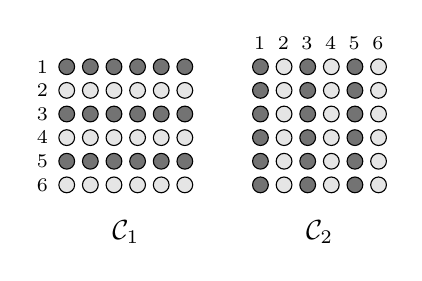
\begin{tikzpicture}[
    poi/.style={circle,draw=black,inner sep=0,minimum size=2mm}
    ]

    % clustering one
    \foreach \y in {0,0.6,1.2} {
      \foreach \x in {0,0.3,0.6,0.9,1.2,1.5} {
        \node[poi,fill=gray!110] at (\x,\y+0.3) {};
        \node[poi,fill=gray!20] at (\x,\y) {};
      }
    }
    % cluster labels
    \foreach \y/\n in {1.5/1,1.2/2,0.9/3,0.6/4,0.3/5,0/6} {
      \node at (-0.3,\y) {$_\n$};
    }

    % clustering label
    \node at (0.75,-0.6) {$\clus_1$};

    % clustering two
    \begin{scope}[xshift=70]
      \foreach \y in {0,0.3,0.6,0.9,1.2,1.5} {
        \foreach \x in {0,0.6,1.2} {
          \node[poi,fill=gray!20] at (\x+0.3,\y) {};
          \node[poi,fill=gray!110] at (\x,\y) {};
        }
      }

      % cluster labels
      \foreach \x/\n in {1.5/6,1.2/5,0.9/4,0.6/3,0.3/2,0/1} {
        \node at (\x,1.8) {$_\n$};
      }

      % clustering label
      \node at (0.75,-0.6) {$\clus_2$};
    \end{scope}

  \end{tikzpicture}
  \caption{Two clusterings, $\clus_1$ and $\clus_2$, formed of six
    clusters each.  These clusterings are optimally different under both the
    assignment metric and variation of information.}
  \label{fig:worst-case}
\end{figure}

Therefore
\begin{equation*}
  \Delta(\clus_1,\clus_2) \leq 2m - \left\lceil \frac{2m}{k} \right\rceil.
\end{equation*}
This bound is tight and can be met with the worst case
\begin{align*}
  \clus_1 = \{&\{1,\dotsc,k\},\{k+1,\dotsc,2k\},\dotsc,\{(k-1)k+1,\dotsc,k^2\}\} \\
  \clus_2 = \{&\{1,k+1,\dotsc,(k-1)k+1\},\\
  &\{2,k+2,\dotsc,(k-1)k+2\},\\
  &\dotsc,\\
  &\{k,k+k,\dotsc,(k-1)k+k\}\}
\end{align*}
which is also shown in Figure~\ref{fig:worst-case}.  This also produces the
worst case under the VI metric, as shown in \citep{meila-2007}.

\section{Worst case performance}
\label{sec:worst-case-perf}

We have so far seen that our two clustering criteria have a number of
similarities, and a number of differences.  Using our metrics for comparing
clusterings, we will now show just how different an all-squares optimal
clustering and a centroid-distance optimal clustering of the same dataset can
be.

\begin{figure}
  \centering
  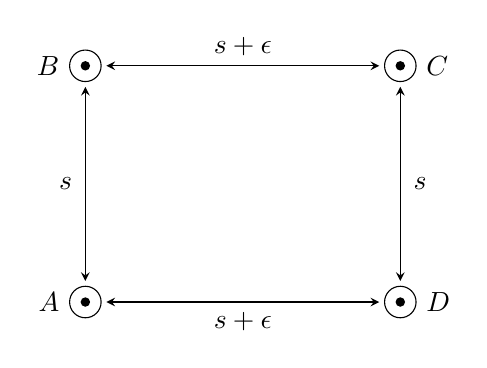
\begin{tikzpicture}[
    >=stealth,
    dot/.style={circle,fill=black,inner sep=0,minimum size=1.2mm},
    sur/.style={circle,fill=white,draw=black,inner sep=0,minimum size=4mm},
    len/.style={<->,shorten >=2mm,shorten <=2mm}
    ]
    % surrounds
    \node[sur,label=left:{$A$}] (A) at (0,0) {};
    \node[sur,label=left:{$B$}] (B) at (0,3) {};
    \node[sur,label=right:{$C$}] (C) at (4,3) {};
    \node[sur,label=right:{$D$}] (D) at (4,0) {};

    % dots
    \node[dot] (A) at (0,0) {};
    \node[dot] (B) at (0,3) {};
    \node[dot] (C) at (4,0) {};
    \node[dot] (D) at (4,3) {};

    % length arrows
    \draw [len] (A) to (B);
    \draw [len] (B) to (D);
    \draw [len] (D) to (C);
    \draw [len] (C) to (A);

    % length labels
    \node at (-0.25,1.5) {$s$};
    \node at (4.25,1.5) {$s$};

    \node at (2,-0.25) {$s+\epsilon$};
    \node at (2,3.25) {$s+\epsilon$};
  \end{tikzpicture}
  \caption{Relative positions of elements to be clustered.  $A$ and $B$
    contain $N$ elements each, $C$ and $D$ contain $N+1$ elements each.}
  \label{fig:clusters}
\end{figure}

Let $(M,d_E)$ be 2-dimensional Euclidean space with the Euclidean metric and
our dataset be $(\dset, \mu_{\dset})$ where $\dset \subset \mathbb{R}^2$,
$\dset = A \cup B \cup C \cup D$, $\mu_{\dset}(A)=\mu_{\dset}(B)=N$ and
$\mu_{\dset}(C)=\mu_{\dset}(D)=N+1$.  The relative positions of $A,B,C,D$ in
the Euclidean plane are shown in Figure~\ref{fig:clusters}.  Two possible
$2$-clusterings of $(\dset,\mu_{\dset})$ are $\{A \cup B,C \cup D\}$ and $\{A
\cup D,B \cup C\}$ which we will call $\clus_1$ and $\clus_2$ respectively.

Formulae for the all-squares and centroid-distance costs of $\clus_1$ and
$\clus_2$ can now be given, first for centroid-distance cost:
\begin{eqnarray*}
  cost_{cd}(\clus_1) &=& \frac{1}{2}\left(Ns^2+(N+1)s^2\right), \\
  cost_{cd}(\clus_2) &=& \frac{1}{2}\left(N(s+\epsilon)^2+(N+1)(s+\epsilon)^2\right).
\end{eqnarray*}
It is clear that $\clus_1$ is the optimal clustering under the
centroid-distance criterion whenever $\epsilon > 0$.  Now, for all-squares
cost,
\begin{eqnarray*}
  cost_{as}(\clus_1) &=& 2N^2s^2+2(N+1)^2s^2, \\
  cost_{as}(\clus_2) &=& 4N(N+1)(s+\epsilon)^2.
\end{eqnarray*}
So $\clus_2$ is the optimal clustering under the all-squares criterion
whenever
\begin{equation*}
  \epsilon < \sqrt{s^2 + \frac{s^2}{2N(N+1)}} - s.
\end{equation*}
Other clusterings of $\dset$ are possible, but these are trivially more
expensive.

A simple numerical example can now be constructed; let $s=1.4$, $\epsilon=0.1$
and $N=1$.  The costs of all possible 2-clusterings are shown in
Table~\ref{tab:costs}.  Again we see that the optimal clustering under each
criterion is different.

% \begin{table}
%   \centering
%   \caption{The costs of possible 2-clusterings
%     of $\dset$, with minimum costs underlined.}
%   \begin{tabular}{lrr}
%   \toprule
%   Clustering & Centroid-distance cost & All-squares cost \\
%   \midrule
%   $\{A \cup B, C \cup D\}$ & \underline{2.94} & 19.6 \\
%   $\{A \cup D, B \cup C\}$ & 3 & \underline{18} \\
%   $\{A \cup C, B \cup D\}$ & $5\frac{46}{75}$ & 33.68 \\
%   $\{A, B \cup C \cup D\}$ & 4.152 & 41.52 \\
%   $\{C, A \cup B \cup D\}$ & 4.2825 & 29.76 \\
%   \bottomrule
% \end{tabular}
% \label{tab:costs}
% \end{table}

\begin{table}
  \centering
  \caption{The costs of possible 2-clusterings
    of $\dset$, with minimum costs underlined.}
  \begin{tabular}{lrr}
  \toprule
  Clustering & Centroid-distance cost & All-squares cost \\
  \midrule
  $\{A \cup B, C \cup D\}$ & \underline{2.940} & 19.60 \\
  $\{A \cup D, B \cup C\}$ & 3.375 & \underline{18.00} \\
  $\{A \cup C, B \cup D\}$ & 5.613 & 33.68 \\
  $\{A, B \cup C \cup D\}$ & 4.152 & 41.52 \\
  $\{B, A \cup C \cup D\}$ & 4.152 & 41.52 \\
  $\{C, A \cup B \cup D\}$ & 4.283 & 29.76 \\
  $\{D, A \cup B \cup C\}$ & 4.283 & 29.76 \\
  \bottomrule
\end{tabular}
\label{tab:costs}
\end{table}


$\clus_1$ and $\clus_2$ are not just slightly different clusterings, they are
in fact optimally different, that is, no two clusterings can be more
different, according to both the VI metric and assignment metric, as well as
our basic intuition.  This leads us to:
\begin{thm}
  \label{thm:worst-case}
  A centroid-distance optimal clustering and an all-squares optimal clustering
  can be optimally different under both the VI metric and the assignment
  metric.
\end{thm}

\section{Conclusion}
\label{sec:conclusion}

In this chapter we have shown that the two sum-of-squares criteria,
centroid-distance and all-squares, share some similarities but also some
differences.  Optimal clusterings according to both criteria may be consistent
but, while centroid-distance always produces linearly separable solutions,
all-squares does not.

Both criteria simultaneously measure both homogeneity and separation.  For
all-squares, the relationship between the homogeneity measure and separation
measure is trivial and independent of the choice of metric.  However, for
centroid-distance we have shown that the homogeneity measure is not
necessarily equivalent to the separation measure when using something other
than the Euclidean metric.  The example we used is the homogeneous
Euclidean-overlap metric for mixed data.

It has recently been shown that the centroid-distance problem is NP-hard using
Euclidean space.  We have shown that both problems are NP-complete even when
using a simple 3-valued metric.  We also show that all-squares is NP-complete
in Euclidean space.  When using a 2-valued metric, both problems are in P,
except for all-squares on a multiset, which remains NP-complete.

We have introduced a new metric for comparing clusterings, called the
assignment metric.  It is, in fact, a family of metrics since any metric for
comparing matched sets can be used.  This allows for some interesting choices
of metric, namely we can use it to compare fuzzy clusterings and take into
account the underlying metric space of the dataset which gives the measure a
more intuitive feel.

We have used this metric to show just how different optimal clusterings
according to the two criteria can be.  It turns out that they can be optimally
different, according to both our metric and the VI metric.

Much of the work here which we present for multisets also applies naturally to
fuzzy multisets.  The consistency results also extend to crispness, that is to
say that optimal fuzzy clusterings according to either criteria need not have
been fuzzy in the first place.  The assignment metric also applies to fuzzy
clusterings simply by using a metric for fuzzy sets.

% Further work will be done on methods for approximating the optimal clustering
% according to all-squares.  Further applications for the assignment metric and
% new bounds will also be investigated.



%%% Local Variables:
%%% TeX-master: "thesis"
%%% End:


\chapter{Hierarchical Clustering}
\label{cha:background2}

\section{Summary}
\label{sec:summary}

In this section we review the relevant terminology and background that is
required for the remainder of this thesis.  We begin with the general theory
of graphs, trees and their relationship to distances and special types of
metrics.  We then look at the problem of reconstructing trees from distances and
finally at the theory of ``lassoing'' a tree from incomplete distance
information.

\section{Graphs, Trees and Distances}
\label{sec:graphs-trees-dist}

\subsection{History}
\label{sec:history}

Trees have been used to represent hierarchical structures for many hundreds of
years \cite{knuth97taocp1}.  One of the most well-known and ubiquitous
occurrences is that of the family tree.  The use of a tree to represent
lineages was widespread in Europe by the 14th Century in Christian artwork
depicting the ancestors of Jesus of Nazareth.  This depiction is known as the
Tree of Jesse \cite{corblet1860etude}.

Darwin would later popularise the concept of the more general ``tree of life''
in his seminal work popularly known as \textit{On the Origin of Species}
\cite{darwin1859origin}.  Darwin's first tree (Figure~\ref{fig:darwin-tree})
shows the theoretical relationship between an ancestral species (1) and its
descendant species \cite{semple2003phylogenetics}.  Extant species are shown
by tips on the endpoints of some branches with the remaining branches possibly
representing extinct species.  His idea was that groups of species would have
diverged at different times and therefore some groups will be more closely
related than others.  For example, the species labelled by B and C would be
more closely related than those labelled by A and D.

\begin{figure}
  \centering
  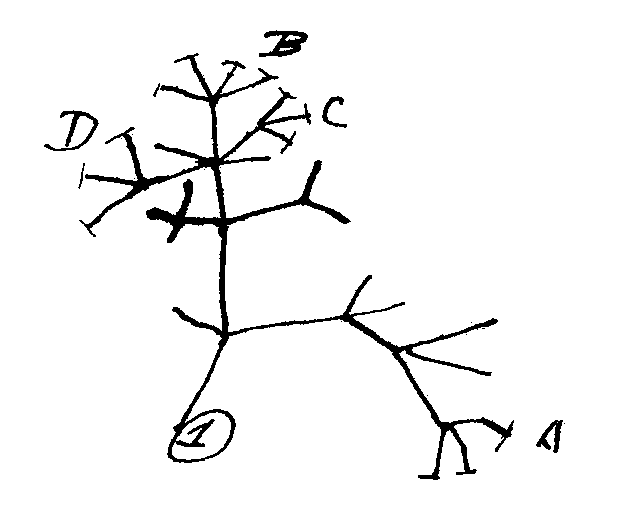
\includegraphics[width=20em]{figures/background2/darwin-tree.png}
  \caption{Charles Darwin's first diagram of an evolutionary tree from his
    notebook \textit{Transmutation of species}, 1837 \cite{darwin1837notebook}.}
  \label{fig:darwin-tree}
\end{figure}

Trees as a formally defined mathematical entity, such as the ones will see in
the following sections, appeared as early as 1847 with the name ``tree''
appearing in the literature shortly afterwards \cite{knuth97taocp1}.  The more
general theory of graphs and topology was developed earlier and is considered
to have begun with Euler who in 1735 presented the paper ``Solutio problematis
ad geometriam situs pertinentis'' \cite{euler1735solutio} in which it was
shown that it was not possible to walk through the city of Königsburg crossing
each of its seven bridges exactly once.

Tree structures are of great importance in computer programming.  One of the
earliest programs to make explicit use of tree structures used them to
represent algebraic formul\ae\ for the purpose of symbolic differentiation
\cite{knuth97taocp1,kahrimanian53differentiation}.  This would later become
the field of computer algebra which would drive the development of computer
science and especially programming languages for many years.

Intuitively, it makes sense to arrange many different types of information in
trees, particularly that for which we can define a distance.  A first question
to ask is whether a representation in terms of a tree exists for a given
dataset and distance function.  As we will see, when the distance function
satisfies certain properties there always exists a tree representation and
this representation is also unique (in a well-defined sense).  We focus then
on a slightly different problem: imagine we know the distance between only
certain pairs of objects in our dataset.  We call this information a partial
distance.  This presents two separate problems.  First, does there exist a
tree representation of a given partial distance and if so, can we find one?
Second, does there exist a unique tree representation of a given partial
distance, and if so can we find it?  These issues are the subject of the
remainder of this thesis.

\subsection{Basic terminology and assumptions}
\label{sec:basic-term-assumpt}

In this section we introduce much of the terminology that is required for
dealing with trees.  Since trees are special cases of graphs, we begin with
general graph theory before moving on to trees and, in particular, a special
type of tree that is of greatest interest to us: the equidistant tree.  As
noted by Knuth \cite{knuth97taocp1} there is a large degree of variation in
the terminology used by different authors in graph theory.  We try to follow
the terminology used in current phylogenetics literature such as
\cite{semple2003phylogenetics} and \cite{dress11lassoing}.  Throughout this
section, let $X$ denote a finite nonempty set.

\subsubsection{Graphs}
\label{sec:graphs}

A \textit{graph} is an ordered pair $(V,E)$ where $V$ is a set of
\textit{vertices} and $E$ is a set (or multiset) of \textit{edges}, each of
the form $\{x,y\}$ such that $x,y \in V$ are distinct.  Unless specified
otherwise, all graphs in this thesis are \textit{simple} and finite meaning
that $V$ and $E$ are finite sets and there are no loops.  Suppose $G = (V,E)$
is a graph. Two vertices $v,v' \in V$ are said to be \textit{adjacent} if
there exists an edge in $G$ joining $v$ and $v'$.  An edge $\{x,y\} \in E$ is
said to be \textit{incident} with the vertices $x$ and $y$.  The
\textit{degree} of a vertex $v \in V$ is the number of edges in $G$ incident
with it.

\begin{figure}
  \centering
  \input{figures/background2/graph-ex.pdft}
  \caption{A graph (i) and a directed graph (ii).}
  \label{fig:graph-ex}
\end{figure}

A \textit{path} is a sequence of distinct vertices $v_1,v_2,\dotsc,v_k$ where
$k \geq 2$ such that for all $i \in \{1,\dotsc,k-1\}, v_i$ and $v_{i+1}$ are
adjacent.  If $k \geq 3$ and $v_1$ and $v_k$ are also adjacent then the path
is called a \textit{cycle}.  A graph is \textit{connected} if between each
pair of distinct vertices there exists a path joining them.  A graph is
\textit{complete} if there is an edge joining each pair of distinct vertices.
A subset $V' \subseteq V$ is called a \textit{clique} if there is an edge
joining each pair of distinct vertices in $V'$.  Figure~\ref{fig:graph-ex}
helps to illustrate these definitions.  In the graph shown in (i) an example
of a path is $g,f,e,d$ and an example of a cycle is $g,f,b,a,g$.  The graph is
connected, but not complete, and the set $\{a,b,g,f\}$ is a clique.

A \textit{directed graph} is an ordered pair $(V,E)$ where $E$ is a set of
\textit{directed edges} or \textit{arcs}.  An arc $(v,v') \in E$ is said to
lead from $v$ to $v'$.  The \textit{out-degree} of a vertex is the number of
arcs leading out from it and the \textit{in-degree} is the number leading in.
The degree of a vertex is therefore the sum of its out-degree and in-degree.
An \textit{oriented path} is a sequence of distinct vertices $v_1,\dotsc,v_k$
such that there exists an arc from $v_i$ to $v_j$ for all $1 \leq i \leq k-1$.
Figure~\ref{fig:graph-ex} (ii) shows a directed graph to help illustrate these
definitions.  Vertex $f$ has out-degree 3, in-degree 1 and therefore degree 4.
An example of an oriented path is $e,f,b,c$.

Two graphs $(V,E)$ and $(V',E')$ are called \textit{isomorphic} if there
exists a bijection $\phi \colon V \to V'$ such that $\{v,v'\} \in E$ if and
only if $\{\phi(v),\phi(v')\} \in E'$.  So, in other words, adjacency of
vertices is preserved.  A graph $(V',E')$ is a \textit{subgraph} of a graph
$(V,E)$ if $V' \subseteq V$ and $E' \subseteq E$.  Further if $V' \subseteq V$
and $E'$ contains all edges $\{v,v'\} \in E$ whenever $v,v' \in V'$ the graph
$(V',E')$ is an \textit{induced subgraph} of $(V,E)$.

\subsubsection{Trees}
\label{sec:trees}

In this section we formally define trees as a special type of graph and
introduce all the relevant terminology for a special type of tree which we
will focus on.

A graph that is connected and has no cycles is called a
\textit{tree}.  Trees can be characterised in many ways, some of which are
given in the following theorem (see \cite[][Section 2.3.4.1]{knuth97taocp1}
for a proof):

\begin{thm}
  If $G$ is a finite graph with $n > 0$ vertices, the following statements are
  equivalent:
  \begin{enumerate}[label=\alph*)]
  \item $G$ is a tree,
  \item $G$ is connected, but if any edge is deleted the resulting graph is no
    longer connected,
  \item There is exactly one path between any two distinct vertices of $G$,
  \item $G$ contains no cycles and has $n-1$ edges,
  \item $G$ is connected and has $n-1$ edges.
  \end{enumerate}
\end{thm}

For example, Figure~\ref{fig:x-tree-ex} shows two graphs which are trees.  The
tree depicted in (ii) is a special type of tree called a \textit{rooted tree}.
A rooted tree (or \textit{oriented tree}) is a directed graph $G$ with a
distinguished vertex $\rho_G$ (the root) such that \cite{knuth97taocp1}:
\begin{enumerate}[label=\alph*)]
\item The root $\rho_G$ has in-degree 0,
\item Each vertex $v$ of $G$ apart from $\rho_G$ has in-degree 1,
\item There is a path between $\rho_G$ and any vertex of $G$ that is not the
  root.
\end{enumerate}

\begin{figure}
  \centering
  \input{figures/background2/x-tree-ex.pdft}
  \caption{A tree (i) and a rooted phylogenetic $X$-tree
    (ii).}
  \label{fig:x-tree-ex}
\end{figure}

Suppose $T$ is a rooted tree.  A vertex in $T$ is called a \textit{leaf} if it
has degree 1.  All other vertices are called \textit{interior} vertices.  An
edge which is incident with a leaf is called a \textit{pendant} edge.  All
other edges are called \textit{interior} edges.  The set of all leaves of $T$
is called the \textit{leafset} of $T$ which we denote by $L(T)$.

Suppose $X$ is a finite, nonempty set, a \textit{rooted phylogenetic $X$-tree}
is a rooted tree with no vertices of in-degree one and out-degree one and with
leafset $X$.  Since the remainder of this thesis is concerned with rooted
trees we will from now on refer to a rooted phylogenetic $X$-tree as simply an
\textit{$X$-tree}.  Figure~\ref{fig:x-tree-ex} (ii) shows an $X$-tree with $X
= \{a,\dotsc,f\}$.

An $X$-tree is \textit{binary} if all interior vertices have degree 3 apart
from the root which has degree 2.  We therefore have that each vertex has
out-degree zero or two and each vertex apart from the root has in-degree 1.
By considering the directed paths from the root to leaves it becomes clear why
such a tree is called binary \cite{semple2003phylogenetics}.

An \textit{edge-weighted graph} $(G,\omega)$ is a graph $G=(V,E)$ paired with
an edge-weighting function $\omega \colon E \to \rr$.  For an edge-weighted
$X$-tree $T$ we call an edge-weighting \textit{proper} if $w(e) > 0$ for every
interior edge $e$ of $T$.

An $X$-tree has a natural partial order on the vertices.  Given an $X$-tree
$T=(V,E)$, a vertex $v \in V$ is an \textit{ancestor} of a vertex $v' \in V$
if and only if $v$ is on the directed path from the root of $T$ to $v'$.  The
vertex $v'$ is then said to be a \textit{descendant} of $v$.  If $v$ and $v'$
are adjacent then we also call $v$ the \textit{parent} of $v'$ and $v'$ a
\textit{child} of $v$.  The number of children of a particular vertex equals
its out-degree.

The \textit{lowest common ancestor} of two vertices $v$ and $v'$ in an
$X$-tree is the unique vertex $u$ such that $u$ is an ancestor of both $v$ and
$v'$ and the path from the root $\rho$ to $u$ is longer than the path to any
other ancestor of both $v$ and $v'$.  The lowest common ancestor of $v$ and
$v'$ is denoted $\lca(v,v')$.  In the $X'$-tree in Figure~\ref{fig:x-tree-ex}
(ii) the lowest common ancestor of $a$ and $d$ is the root $\rho$.

A connected subgraph of a tree is called a \textit{subtree}.  If $T$ is an
$X$-tree and $X' \subseteq X$ then we denote by $T|X'$ the subtree of $T$
whose leafset is $X'$, with degree 2 vertices suppressed.  $T|X'$ is then
called a \textit{restricted subtree}.  If $T$ is binary and $|X'| = 3$ then
$T|X'$ is called a \textit{triplet}.

We call two $X$-trees $T$ and $T'$ \textit{equivalent} (written $T \simeq T'$)
if there exists a bijection $\phi \colon V(T) \to V(T')$ that extends to a
graph isomorphism that is the identity on $X$.  Since an $X$-tree is rooted,
$\phi$ must also map $\rho_{T}$ to $\rho_{T'}$.

For a set $X$ the number of possible non-equivalent binary $X$-trees is
$(2|X|-3)!!$ (where $!!$ means double factorial).  Therefore to find a tree in
this space with particular properties we cannot look at each possible tree and
must instead use a special tree reconstruction method.  Next we look at how
distances are related to trees and then at the problem of reconstructing a
tree from distance information.

\subsubsection{Ultrametrics}
\label{sec:ultrametrics}

Given an edge-weighted $X$-tree $(T,\omega)$ where $T=(V,E)$ and $\omega
\colon E \to \rrnn$ we can associate a distance $D_{(T,\omega)} \colon X
\times X \to \rrnn$ to $(T,\omega)$ by setting for all $x,y \in X$:
\begin{equation*}
  D_{(T,\omega)}(x,y) =
  \begin{cases}
    \displaystyle
    \sum_{e \in P(x,y)} \omega(e) & \text{if $x \neq y$},\\
    0 & \text{otherwise,}
  \end{cases}
\end{equation*}
where $P(x,y)$ is the set of edges on the path from $x$ to $y$.  We call
$D_{(T,\omega)}$ the distance \textit{induced} by $(T,\omega)$.

\begin{figure}
  \centering
    \begin{subfigure}[b]{0.5\textwidth}
      \centering
      \input{figures/background2/treeconstruct1.pdft}
      \label{fig:example-equidistant-1}
      \caption{}
    \end{subfigure}%
    ~
  \begin{subfigure}[b]{0.5\textwidth}
    \centering
    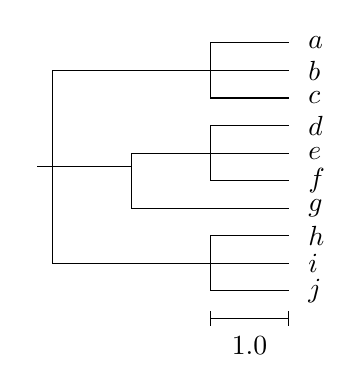
\begin{tikzpicture}[yscale=0.35]
    \node (r) at (0.0,0.0) {};
\node (rr) at (-0.2,0.0) {};
\draw (r.center) -- (rr.center);
\node (r1) at (2.0,-3.5) {};
\node[label=right:{$j$}] (r11) at (3.0,-4.5) {};
\draw (r1.center) |- (r11.center);
\node[label=right:{$i$}] (r12) at (3.0,-3.5) {};
\draw (r1.center) |- (r12.center);
\node[label=right:{$h$}] (r13) at (3.0,-2.5) {};
\draw (r1.center) |- (r13.center);
\draw (r.center) |- (r1.center);
\node (r2) at (1.0,0.0) {};
\node[label=right:{$g$}] (r21) at (3.0,-1.5) {};
\draw (r2.center) |- (r21.center);
\node (r22) at (2.0,0.5) {};
\node[label=right:{$f$}] (r221) at (3.0,-0.5) {};
\draw (r22.center) |- (r221.center);
\node[label=right:{$e$}] (r222) at (3.0,0.5) {};
\draw (r22.center) |- (r222.center);
\node[label=right:{$d$}] (r223) at (3.0,1.5) {};
\draw (r22.center) |- (r223.center);
\draw (r2.center) |- (r22.center);
\draw (r.center) |- (r2.center);
\node (r3) at (2.0,3.5) {};
\node[label=right:{$c$}] (r31) at (3.0,2.5) {};
\draw (r3.center) |- (r31.center);
\node[label=right:{$b$}] (r32) at (3.0,3.5) {};
\draw (r3.center) |- (r32.center);
\node[label=right:{$a$}] (r33) at (3.0,4.5) {};
\draw (r3.center) |- (r33.center);
\draw (r.center) |- (r3.center);
\draw[|-|] (2.0,-5.5) -- (3.0,-5.5);
\node at (2.5,-6.5) {1.0};
     \end{tikzpicture}
     \caption{}
     \label{fig:example-equidistant-2}
   \end{subfigure}

   \caption{A dendrogram is a visual representation of a tree.  Here we see
     two different ways to draw the same edge-weighted $X$-tree.}
   \label{fig:example-equidistant}
\end{figure}

The distance induced by a tree is a special type of metric called a
\textit{tree metric}.  These metrics have some interesting properties which
are discussed in \cite[Chapter 7]{semple2003phylogenetics}.  For our purposes
we are most interested in a special type of tree metric called an
\textit{ultrametric}.  A distance $\delta \colon X \times X \to \rr$ is called
an ultrametric if for every distinct $x,y,z \in X$ the following stronger form
of the triangle inequality holds:
\begin{equation*}
  \delta(x,y) \leq \max(\delta(x,z),\delta(y,z)).
\end{equation*}

An edge-weighting $\omega \colon E \to \rr$ for an $X$-tree $T=(V,E)$ with
root $\rho_T$ is called \textit{equidistant} if it satisfies the following
properties:
\begin{itemize}
\item[(i)] $D_{(T,\omega)}(\rho_T,x) = D_{(T,\omega)}(\rho_T,y)$ for all $x,y
  \in X$,
\item[(ii)] $D_{(T,\omega)}(x,y) \geq D_{(T,\omega)}(x,u)$ for all $x \in X$
  and any $u,v \in V$ whenever $u$ is encountered before $v$ on the directed
  path from $x$ to $\rho$.
\end{itemize}
If $\omega$ is an equidistant edge-weighting then $D_{(T,w)}$ is an
ultrametric \cite[Lemma 7.2.4]{semple2003phylogenetics}.  $X$-trees with
equidistant edge-weightings arise naturally in many places, for example in
phylogenetics.  For convenience we will from now on refer to such an $X$-tree
with equidistant edge-weighting as simply an \textit{equidistant $X$-tree}.

Figure~\ref{fig:example-equidistant} shows an example of an equidistant
$X$-tree with $X = \{a, \dotsc, j\}$ using two common display formats
(dendrograms).  In (i) the edges are simply labelled with their weights (edges
with weight 1 are left unlabelled for clarity).  In (ii) the weight of each
edge is proportional to the horizontal component of its length on the bar with
the actual length shown with a scale bar.

For any ultrametric $\delta \colon X \times X \to \rr$ there is, up to
isomorphism, a unique equidistant $X$-tree $(T,\omega)$ such that $\delta(x,y)
= D_{(T,\omega)}(x,y)$ for all $x,y \in X$.  This tree can be recovered from
the ultrametric in polynomial time, as we will see in the next section.

\section{Tree reconstruction}
\label{sec:tree-construction}

In this section, we look at various methods of reconstructing trees.  Of most
interest to us is the problem of reconstructing an $X$-tree from a distance on
$X$.  This is generally done by one of two broad classes of hierarchical
clustering methods which we discuss in Section~\ref{sec:hier-clust-meth}.

A further problem is that of reconstructing an edge-weighted $X$-tree from a
distance on $X$.  This is desirable in many cases, for example in
phylogenetics the edge-weights might represent the time or number of point
mutations \cite{felsenstein2004inferring}.

Closely related to this is the problem of reconstructing $X$-trees from only
partial distance information.  This means that we do not have the complete
distance $d$, but rather only have the values $d(x,y)$ for some, but not all,
pairs $x,y \in X$.  This problem is motivated by the fact that accurate
distance measurements are often difficult or impossible to obtain in practice
but one would still like to build an edge-weighted $X$-tree given only what is
known.

As with complete distance information, it is possible for partial distance
information to uniquely determine an $X$-tree.  This is the subject of
Section~\ref{sec:lassoing-corralling}.  This allows us to define a consistency
property for partial distance reconstruction methods.

\subsection{Reconstruction from subtrees}
\label{sec:constr-from-subtr}

Before we look at reconstructing trees from distances, it is interesting to
note that we do not actually need a distance to reconstruct only the topology
of an $X$-tree.  It suffices merely to know the set of subtrees displayed by
the tree \cite{semple2003phylogenetics}.

A pair of leaves of an $X$-tree that share the same parent is called a
\textit{cherry} and a set of leaves (of any size) that share the same parent
is called a \textit{pseudocherry}.  As before, an $X$-tree with $|X| = 3$ that
contains a cherry is called a triplet.  If $P$ is an $\{a,b,c\}$-tree $a,b$ is
a cherry of $P$ then we denote the triplet $P$ by $ab|c$.  We say that a
triplet $ab|c$ is \textit{displayed} by an $X$-tree $T$ if the restriction
$T|\{a,b,c\}$ of $T$ to $\{a,b,c\}$ is binary and $lca_T(a,c) = lca_T(b,c)$ is
an ancestor of $lca_T(a,b)$ in $T$.  For example, the tree $T_2$ in
Figure~\ref{fig:build-ex} is a triplet and can be written as $ad|c$.

\begin{figure}
  \centering
  \input{figures/background2/build-ex2.pdft}
  \caption{An illustration of \textsc{Build} with an input of $R =
    \{T_1,T_2\}$.  $[R,S]$ is the auxiliary graph built in the first iteration
    of the algorithm and $T$ is the final tree constructed.}
  \label{fig:build-ex}
\end{figure}

The \textsc{Build} algorithm \cite{aho1981inferring} can be used to
reconstruct an $X$-tree $T$ from the set of all triplets displayed by $T$.  We
show the \textsc{Build} algorithm in pseudocode in Algorithm~\ref{alg:build}
and give an example in Figure~\ref{fig:build-ex}.  The algorithm uses a set
$R$ of rooted trees $\{T_1,\dotsc,T_n\}$ where $L(T_1) \cup \dotsb \cup L(T_n)
= X$ and an auxiliary graph $[R,S]$ which has vertex set $S \subseteq X$ and
an edge $\{a,b\}$ for each $a,b \in S$ whenever there exists some $c \in S$
and some $T' \in R$ such that $T'|\{a,b,c\}$ and $ab|c$ are equivalent.

\begin{algorithm}
  \caption{\textsc{Build}.}
  \label{alg:build}

  \begin{algorithmic}
    \Require A set of rooted trees $R = \{T_1,\dotsc,T_n\}$.
    \Ensure  An $X$-tree $T$ where $X = L(T_1) \cup \dotsb \cup L(T_n)$.

    \State $S = \{x_1,\dotsc,x_m\} \gets X$.

    \If{$|S| = 1$} \Return the tree $(\{x_1\},\emptyset)$. \EndIf

    \If{$|S| = 2$} let $\rho$ be a new vertex and \Return the tree with root
    node $\rho$ obtained by attaching $x_1$ and $x_2$ to $\rho$. \EndIf

    \State Construct the auxiliary graph $[R,S]$.

    \State Let $S_1,\dotsc,S_k$ be the vertex sets of the connected components
    of $[R,S]$.

    \ForAll{$1 \leq i \leq k$}
    \State Let $T_i$ be the output of \textsc{Build} on $R_i =
    \{T|S_i \colon T \in R\}$.
    \EndFor

    \State Let $\rho$ be a new vertex and \Return the tree with root node
    $\rho$ obtained by attaching the root of each $T_i$ to $\rho$.
    
  \end{algorithmic}
\end{algorithm}

This algorithm has some nice properties, for example if \textsc{Build} returns
a tree then the set of input trees is said to be \textit{compatible}.  The
definition of compatible is independent of \textsc{Build} (see
\cite{semple2003phylogenetics}) but \textsc{Build} can be used to check
compatibility.  Furthermore, if we input the set of all triplets displayed by
a tree $T$, then \textsc{Build} is guaranteed to output $T$ and therefore $T$
is uniquely determined by the set of triplets it displays.

If the inputted set of triplets $R$ is some subset of all the triplets
displayed by a tree then the set is still compatible but this set is displayed
by possibly many trees.  In this case the output of \textsc{Build} is
deterministic and the tree reconstructed is known as \textit{the
  \textsc{Build} tree for $R$}.  Some interesting properties of these trees
can be found in \cite[Section 2.5.2]{bryant97buildingtrees}.

The \textsc{Build} algorithm was initially developed to construct a tree
satisfying a given set of constraints and was applied to problems arising in
the theory of relational databases.  It was later applied to phylogenetics but
remained relatively unknown in the field for a number of years
\cite{steel1992complexity,bryant04supertree}.

When the inputted trees are not compatible, \textsc{Build} returns an error.
Since it is often the case that trees will not be compatible, the
\textsc{MinCutSupertree} algorithm was developed which will construct a tree
even if the input trees are not compatible \cite{semple2000supertree}.
The algorithm builds a graph similar to $[R,S]$ and ensures that it is
disconnected in each step by using a minimum cut.  This algorithm was
developed primarily for construction of phylogenetic supertrees.

\subsection{Reconstruction from distances}
\label{sec:constr-from-dist}

We now turn to the problem of reconstructing an $X$-tree from a distance.  We
begin with a brief overview of general hierarchical clustering methods and
then look at the UPGMA method \cite{sokal1958statistical} and its optimal
runtime algorithm.  Hierarchical clustering methods in general build
unweighted $X$-trees, but UPGMA can be considered an extension which also
constructs an edge-weighting for the constructed tree.

For a distance-based reconstruction method the following property is
desirable: if we input a distance function $D_{(T,\omega)}$ induced by an
edge-weighted $X$-tree $(T,\omega)$ we get the tree $T$ and its edge-weighting
$\omega$.  If a method enjoys this property then we call it
\textit{consistent}.  For many methods this property holds only under certain
conditions.  For UPGMA this holds if $(T,\omega)$ is a binary equidistant
$X$-tree \cite{durbin1998biological}.

\subsubsection{Hierarchical clustering methods}
\label{sec:hier-clust-meth}

\begin{figure}
  \centering
  \input{figures/background2/tree-clust-ex.pdft}
  \caption{A tree can be viewed as a hierarchy of partitions.}
  \label{fig:tree-clust-ex}
\end{figure}

Hierarchical clustering is used for the classification of information in much
the same way as partitional clustering.  The aim of a hierarchical clustering
method is to produce an $X$-tree corresponding to a given distance $D$ on a
set $X$.  While a partition of a set is merely a set of disjoint subsets
(clusters) which ``cover'' the set, an $X$-tree can be viewed as a hierarchy
of such clusters which induces several partitions on $X$.  This natural
relationship between trees and partitions is illustrated in
Figure~\ref{fig:tree-clust-ex}.  In the example we have $X = \{a,\dotsc,e\}$.
The root of the tree corresponds to the single cluster $X$ (denoted $abcde$)
and as we move down the tree the set is partitioned further until we have
cluster of one leaf each ($\{\{a\},\dotsc,\{e\}\}$, denoted $a|b|c|d|e$ for
short).

There are two main methods in use for building hierarchies.  These are the
\textit{agglomerative} or ``bottom-up'' methods which begin with each element
of $X$ in its own cluster and successively merges clusters until there is only
one cluster left, and the \textit{divisive} or ``top-down'' methods which
begin with a single cluster and successively splits clusters until each
element is on its own.  The resulting hierarchy depends upon which merges or
splits have been chosen at each stage which, in turn, depends on finding a
local optimum according to some criterion.

\begin{algorithm}[h]
  \caption{Agglomerative hierarchical clustering algorithm.}
  \label{alg:agglomerative}

  \begin{algorithmic}
    \Require A set $X$ and a linkage function $D \colon 2^X \times 2^X \to \rr$
    with an underlying distance $d \colon X \times X \to \rr$.

    \Ensure  A rooted $X$-tree $T$.

    \State Let $F$ be a forest of $|X|$ trees each containing a unique element
    of $X$ as the only vertex, which is also the root,

    \While{$|F| > 1$}

       \State Let $v$ be a new vertex and $\displaystyle (x,y) \gets \argmin_{x,y
         \in F} D(L(x),L(y))$,
       \State Remove trees $x$ and $y$ from $F$ and add the tree obtained by
         attaching the roots of $x$ and $y$ to $v$ and letting $v$ be the root,
    
    \EndWhile

    \State \Return the single tree contained in $F$.
    
  \end{algorithmic}
\end{algorithm}

The general algorithm for agglomerative clustering is shown in
Algorithm~\ref{alg:agglomerative}.  The choice of linkage function determines
how the distances are recomputed at each stage and therefore which trees are
joined in each subsequent stage.  Given a set $X$ and distance $d \colon X
\times X \to \rr$ and two nonempty subsets $C_1,C_2 \subseteq X$, some common
choices for linkage functions include:\\
single-linkage:
\begin{equation*}
  \label{eq:slink}
  D_{SL}(C_1,C_2) = \min_{x \in C_1, y \in C_2} d(x,y),
\end{equation*}
complete-linkage:
\begin{equation*}
  \label{eq:clink}
  D_{CL}(C_1,C_2) = \max_{x \in C_1, y \in C_2} d(x,y),
\end{equation*}
and average-linkage:
\begin{equation*}
  \label{eq:alink}
  D_{AL}(C_1,C_2) = \left(\,\sum_{x \in C_1} \sum_{y \in C_2} d(x,y) \right) / |C_1| |C_2|.
\end{equation*}

The general algorithm for agglomerative clustering has runtime complexity of
$O(n^3)$ where $n = |X|$ since there are $O(n)$ merges to be done and finding
the $\argmin$ takes $O(n^2)$ time.  However, for many linkage criteria,
including the three above, it is possible to use an $O(n^2)$ algorithm.  Two
well known examples are SLINK \cite{sibson1973slink} and CLINK
\cite{defays1977efficient} for using single-linkage and complete-linkage
respectively.  In the next section we will see that hierarchical clustering
using average-linkage may be done in quadratic time too.

The divisive method works in the opposite direction: we begin with a single
cluster and successively split clusters until we end up with one cluster per
leaf.  Divisive methods are usually significantly more complicated than
agglomerative methods.  Each step requires an initial decision about which
cluster to split, and then a decision about how to split that cluster
\cite{savaresi2002cluster}.  A naïve approach for deciding which cluster to
split next is to always split the largest cluster, but there are more
sophisticated approaches, for example based on cluster homogeneity.  Splitting
a cluster then essentially requires a partitional clustering method
\cite{ding2002cluster}.  In general the time complexity of a divisive method
is $O(2^n)$ where $n = |X|$ making it prohibitively expensive for most
applications \cite{cimiano2004comparing}.

\subsubsection{UPGMA}
\label{sec:upgma}

Unweighted Pair Group Method with Arithmetic Mean (UPGMA)
\cite{sokal1958statistical} is in fact a modified agglomerative clustering
method using average-linkage which reconstructs an equidistant $X$-tree.  For
an equidistant $X$-tree $(T,\omega)$, let $height((T,\omega))$ be the sum of
the edge weights on the path from the root of $T$ to any leaf, or 0 if the
root is the sole vertex.  The algorithm for UPGMA is shown in
Algorithm~\ref{alg:upgma}.

\begin{algorithm}[h]
  \caption{UPGMA.}
  \label{alg:upgma}

  \begin{algorithmic}
    \Require A set $X$, and a distance $d \colon X \times X \to \rr$.
    \Ensure  A binary equidistant $X$-tree $(T, \omega)$.

    \State Let $F$ be a forest of $|X|$ trees each containing a unique element
    of $X$ as the only vertex, which is also the root.

    \While{$|F| > 1$}

       \State Let $v$ be a new vertex,
       \State put $\displaystyle m \gets \min_{x,y \in F} D_{AL}(L(x),L(y))$,
       \State and $\displaystyle (x,y) \gets \argmin_{x,y \in F} D_{AL}(L(x),L(y))$.
       \State Remove trees $x$ and $y$ from $F$ and add the tree obtained by
         attaching the root of $x$ to $v$ with an edge of length $m/2 -
         height(x)$, attaching the root of $y$ to $v$ with an edge of length
         $m/2 - height(y)$ and letting $v$ be the root.
    
    \EndWhile

    \State \Return the $X$-tree contained in $F$ and its edge-weighting.
  \end{algorithmic}
\end{algorithm}

Since only two trees are joined in each iteration, the output of UPGMA is
always a binary tree.  If the input distance $d$ is equal to the induced
distance $D_{(T,\omega)}$ of some equidistant binary $X$-tree $(T,\omega)$
then UPGMA is guaranteed to return $(T,\omega)$ \cite{durbin1998biological}.

% mention general method for other linkage criteria

% However, for all three of the linkage
% functions above there are special algorithms which run in only $O(n^2)$ time,
% these are SLINK \cite{sibson1973slink}, CLINK \cite{defays1977efficient} and
% UPGMA respectively.  The following section discusses .

In the general agglomerative algorithm, each step involves identifying a pair
of elements such that no other pair of elements in $X$ are closer according to
the chosen linkage criterion.  In other words, we are finding a global
minimum.  In more efficient algorithms we instead look only for a local
minimum at each stage.  A local minimum in this context means a pair of
elements which are \textit{mutual nearest neighbours} (MNNs).  Given a set $X$
and a distance $d$ on $X$, a pair $x,y \in X$ are MNNs if there exists no
element $z \in X$ for which $d(x,z) < d(x,y)$ or $d(y,z) < d(x,y)$.  Such a
pair can be safely agglomerated as soon as it is found, just as in the general
algorithm \cite{murtagh2011methods}.

Finding MNNs can be done quickly by building a chain of nearest neighbours in
the following way: we begin with an arbitrary cluster in $X$ and find its
nearest neighbour giving us a chain of length two.  We then repeatedly add to
the chain the nearest neighbour of the last element in the chain until we find
a pair of MNNs.  The MNNs are removed from the chain and agglomerated.  The
distances between new clusters and all other clusters are calculated
recursively using the Lance-Williams update formula in constant time
\cite{lance66theory}.  The process is then continued from the end of the
chain, or from an arbitrary cluster if the chain is empty.  This method works
because for certain linkage criteria, including average-linkage, the nearest
neighbour chain remains valid after an agglomeration (see
\cite{gronau2007optimal} for details).

This mutual nearest neighbour method, also called the \textit{algorithme des
  célibataires}, was developed in the early 1980s and initially appeared in
\cite{de1980classification} and \cite{juan1982programme} (in French) and later
in \cite{murtagh1983survey} and \cite{murtagh1984complexities} (in English).
It leads to the optimal $O(n^2)$ version of UPGMA and other hierarchical
clustering methods \cite{gronau2007optimal}.

\subsection{Reconstruction from partial distances}
\label{sec:constr-from-part}

Partial distances arise often in practice, that is a distance where the
distance between some pairs of elements is missing.  Potential reasons for
this might be that it is sometimes difficult or impossible to make
measurements between certain pairs due to those pairs not sharing any
information from which a distance can be inferred.  For example, in biological
studies involving large numbers of species and genes it is often the case that
species do not share any genes in the available data
\cite{criscuolo2008fastnj}.  We discuss the motivation for studying this
problem in more detail in Section~\ref{sec:lasso-motivation}.

For this reason it becomes useful to ask whether a partial distance can be
extended into a complete distance that is also an ultrametric.  More formally,
a \textit{partial distance} on $X$ is a function $d^* \colon (X \times X) - M
\to \rrnn$ where $M$ is the set of pairs for which the distance value is
missing.  The problem is to find a complete distance $d \colon X \times X \to
\rrnn$ where $d(x,y) = d^*(x,y)$ for all $x,y \in (X \times X) - M$ and which
is an ultrametric.  In \cite{farach1995robust} it was shown that it is
possible to decide in polynomial time whether an extension to an ultrametric
exists (and to compute such an extension), although the corresponding decision
problem for unrooted trees (that is, deciding if an extension to a general
tree metric exists) is NP-complete.

Below we describe three different methods proposed in the literature for
extending a partial distance on $X$ to an ultrametric on $X$ and
reconstructing the corresponding equidistant $X$-tree.  We restrict ourselves
to equidistant $X$-trees but similar results on unrooted trees may be found
in, for example, \cite{guenoche1999approximations}, \cite{farach1995robust},
\cite{makarenkov2001nouvelle} and \cite{guenoche2004extension}.

\subsubsection{An optimisation method}
\label{sec:part-dist-optim-method}

The approach taken by \citet{de1984ultrametric} is to consider a least squares
constrained optimisation problem.  Given a partial distance $d^* \colon (X
\times X) - M \to \rrnn$, a function $Loss \colon \rrnn^{X \times X} \to
\rrnn$ (where $\rrnn^{X \times X}$ is the set of all dissimilarities on $X$)
is defined as:
\begin{equation*}
  \label{eq:partial-dist-least-squares}
  Loss(d) = \sum_{(x,y) \in (X \times X) - M} \!\big(d^*(x,y)-d(x,y)\big)^2.
\end{equation*}
This is called the \textit{loss function}.  The problem is now to find a
function $d \colon X \times X \to \rrnn$ such that $Loss(d)$ is minimised and
with the constraint that $d$ is an ultrametric.

To solve the constrained minimisation problem the authors propose to use the
sequential unconstrained minimisation technique (SUMT)
\cite{fiacco1964sequential}.  Under this technique the constraint that $d$ be
an ultrametric is removed and instead we find a distance $d_n \colon X \times
X \to \rrnn$ which minimises the augmented function $\Phi \colon \rrnn^{X
  \times X} \times \rrnn \to \rrnn$ defined as:
\begin{equation*}
  \label{eq:partial-dist-optimisation}
  \Phi(d_n,\sigma) = Loss(d_n) + \sigma Pen(d_n), \qquad (\sigma > 0),
\end{equation*}
where $Loss$ is the loss function and $Pen \colon \rrnn^{X \times X} \to
\rrnn$ is called the \textit{penalty function} which is meant to enforce the
ultrametric condition.  $Pen$ is defined as:
\begin{equation*}
  \label{eq:penalty-function}
  Pen(d_n) = \sum_{(i,j,k) \in \Omega(d_n)} \! \big(d_n(i,k) - d_n(j,k)\big)^2
\end{equation*}
where
\begin{equation*}
  \Omega(d_n) = \{(i,j,k) \in X^3 \colon d(i,j) \leq \min\big(d_n(i,k),d_n(j,k)\big)
  \text{ and } d_n(i,k) \neq d_n(j,k)\}.
\end{equation*}
In other words, $\Omega(d_n)$ denotes the set of $3$-tuples for which the
ultrametric condition is violated.  The unconstrained minimisation is
performed successively with an increasing value for $\sigma$, each time using
the previous result $d_{n-1}$ to begin the search for the next $d_n$.  A
method by \cite{powell1977restart} is used to perform the unconstrained
minimisation.

\subsubsection{An agglomerative method}
\label{sec:part-dist-agglom-method}

Missing Values Linkage (MVL) is an example of an agglomerative approach
proposed by \cite{schader1992mvl}.  It is actually identical to the
agglomerative hierarchical clustering algorithm (see
Section~\ref{sec:hier-clust-meth}) but using a linkage criterion modified to
take into account missing values.

The modified
average-linkage criterion for two nonempty sets $S_1, S_2$ is:
\begin{equation*}
  D_{MVL}(S_1,S_2) =
  \begin{cases}
    \displaystyle
    \frac{\displaystyle \sum_{(x,y) \in (S_1 \times S_2) - M} d(x,y)}
         {|(S_1 \times S_2) - M|} & \text{if $(S_1
      \times S_2) - M \neq \emptyset$,} \\
    \infty & \text{otherwise},
  \end{cases}
\end{equation*}
where $M = \{(i,j) \in X \times X \colon d(i,j) \text{ is unknown}\}$.
Modified versions of other linkage criteria are possible; some more examples
are given in the original paper.

The authors do not provide an algorithm with better time complexity than that
of the naïve $O(n^3)$ agglomerative algorithm (where $n = |X|$).  They also
show that the MVL method produces very similar results to
\citeauthor{de1984ultrametric}'s method.

Figure~\ref{fig:farach-mvl-ex} (ii) shows the tree constructed by MVL from a
partial distance $d$ on a set $\{a,\dotsc,e\}$ containing only the distances
$d(a,b)=1, d(b,c)=1, d(c,d)=2, d(c,e)=2, d(d,e)=3$.

\subsubsection{A divisive method}
\label{sec:part-dist-divisive-method}

\citet{farach1995robust} use a top down, divisive approach.  Given a partial
distance function $d^* \colon (X \times X) - M \to \rrnn$ let $G=(V,E)$ be a
graph with vertex set $X$ and an edge $\{x,y\}$ with $x,y \in X$ but $(x,y)
\notin M$ (so the distance between $x$ and $y$ is known).  We also define an
edge-weighting $\omega \colon E \to \rr$ by $\omega(\{x,y\}) = d^*(x,y)$ for
all $x,y \in E$.

The tree reconstruction algorithm proceeds as follows:
\begin{enumerate}
\item If $E = \emptyset$, return the single element in $V$.
\item Otherwise, put $m \gets max_{e \in E} \omega(e)$.
\item Let $G^* = (V,E^*)$ be a graph and put $E^* \gets \{e \in E \colon
  \omega(e) < m\}$.
\item Let $u$ be a new vertex and return the tree with root node $u$ obtained
  by recursing on each connected component of $G^*$ and attaching the results
  of each to $u$.               %what if only one component?!
\end{enumerate}
This basic algorithm shown here requires $O(|V||E|)$ time but a quicker
algorithm requiring only $O(|E| + |V|\log |V|)$ time is also given by
\cite{farach1995robust}.

Figure~\ref{fig:farach-mvl-ex} (i) shows the tree constructed by this method
from the same partial distance $d$ on $\{a,\dotsc,e\}$ containing only the
distances $d(a,b)=1, d(b,c)=1, d(c,d)=2, d(c,e)=2, d(d,e)=3$.  Note that the
tree constructed is different to the tree constructed by MVL.

\begin{figure}
  \centering
  \input{figures/background2/farach-mvl-ex.pdft}
  \caption{The two different trees constructed by Farach's method (i) and the
    MVL method (ii) from the same partial distance information.}
  \label{fig:farach-mvl-ex}
\end{figure}

\section{Lassos}
\label{sec:lassoing-corralling}

As we saw in the example shown in Figure~\ref{fig:farach-mvl-ex}, the existing
partial distance reconstruction methods can construct different trees from the
same input.  The problem with the example partial distance in that case was
that no ultrametric extension exists so the methods each modified the given
distances in different ways to obtain an ultrametric.  This means that for
some pairs of leaves in the resulting tree the induced tree distance is not
equal to the inputted distance.  This may be undesirable.

A second problem is that often more than one extension to an ultrametric is
possible.  We will see this in the example in the following section.  In the
case where more than one extension is possible the existing algorithms will
provide one of many solutions.  But we may wish to know not only that an
ultrametric extension exists but that it is unique.  This section provides us
with some theory for deciding when this is possible.

Certain partial distances on $X$ have the property that they uniquely
determine the topology or edge-weights of an $X$-tree.  In other words, only
one extension to an ultrametric on $X$ is possible.  To enable us to
understand when partial distances have this uniqueness property, the theory of
lassos was developed.  We next define certain types of lassos as applied to
equidistant $X$-trees and look at some important characterisations.

\subsection{Definitions and basic properties}
\label{sec:defin-basic-prop}

Let $(T,\omega)$ and $(T',\omega')$ be two edge-weighted $X$-trees and $\cL
\subseteq {X \choose 2}$ be some subset of pairs of elements in $X$.  For
convenience we denote an element $\{x,y\} \in \cL$ as simply $xy$.  Then
$(T,\omega)$ and $(T',\omega')$ are called \textit{$\cL$-isometric} if
$D_{(T,\omega)}(x,y) = D_{(T',\omega')}(x,y)$ for all $xy \in \cL$.

Now, given an $X$-tree $T$ and a subset $\cL \subseteq {X \choose 2}$ we
define $\cL$ to be:
\begin{enumerate}[label=(\roman*)]
\item an \textit{equidistant lasso} for $T$ if $\omega = \omega'$ holds for
  all equidistant edge-weightings $\omega,\omega'$ of $T$ where $(T,\omega)$
  and $(T,\omega')$ are $\cL$-isometric,
\item a \textit{topological lasso} for $T$ if $T$ is equivalent to $T'$ for
  any $X$-tree $T'$ for which there exist proper edge-weightings $\omega$ and
  $\omega'$ of $T$ and $T'$ respectively where $(T,\omega)$ and $(T',\omega')$
  are $\cL$-isometric,
\item a \textit{strong lasso} $T$ if $\cL$ is both an equidistant and
  topological lasso for $T$.
\end{enumerate}

\begin{figure}
\begin{center}
\input{figures/background2/lasso-example.pdft}
\end{center}
\caption{Two equidistant $X$-trees.  All edges have weight 1 except bold edges
  which have weight 2.  For $\cL=\{ac,de,bc,ce,cd\}$ both trees induce the
  same distances over the cords in $\cL$ despite having different topologies.
  In this case $\cL$ is not a topological lasso.}
\label{fig:lasso-example}
\end{figure}

To illustrate these concepts consider the two equidistant $X$-trees
$(T,\omega)$ and $(T',\omega')$ depicted in Figure~\ref{fig:lasso-example}.
The edge-weights on the edges are proportional to the length of the edges as
shown and induce distances $D_{(T,\omega)} \colon X \times X \to \rr$ and
$D_{(T',\omega')} \colon X \times X \to \rr$ respectively.  The trees are
therefore equidistant.  If we have the set of cords $\cL=\{ac,de,bc,ce,cd\}$
then notice that the distances between each of these pairs of leaves is the
same according to the induced distances for both trees (for example
$D_{(T,\omega)}(a,c) = D_{(T',\omega')}(a,c)$).  Therefore $\cL$ is not a
topological lasso.  Notice that this property of $\cL$ is dependent solely on
the structure of the set itself and not on the actual distances on the trees.
For further information and discussion about lassos, especially those
concerning more general trees, the reader is referred to
\cite{dress11lassoing} and \cite{huber2014tree}.

\subsection{Characterising lassos: the child-edge graph}
\label{sec:lassoing-rooted-x}

Lassos for $X$-trees can be characterised using a graph associated to each
interior vertex of a tree \cite{huber13lassoing}.  First, a lasso $\cL$ of $X$
which satisfies the property that $\bigcup_{c \in \cL} c = X$ is called a
\textit{covering} of $X$.  Let $T$ be an $X$-tree and $\iV(T)$ denote the set
of internal vertices of $T$.  For some $v \in \iV(T)$, and a set of cords $\cL
\subseteq {X \choose 2}$, we associate a graph called $G(\cL,v)$ defined as
follows.  The vertex set of the graph $V_v$ is the set of all child edges of
$v$.  The edge set $E_v$ is the set of all $\{e,e'\} \in {V_v \choose 2}$ for
which there exist leaves $a,b \in X$ and a cord $ab \in \cL$ such that $e$ and
$e'$ are edges on the path from $a$ to $b$ in $T$.  We call the graph
$G(\cL,v)$ the \textit{child-edge graph} (\textit{of $v$ with respect to $T$
  and $\cL$}).

We have the following characterisation of topological lassos which originally
appeared in \cite{huber13lassoing}:
\begin{thm}
  \label{thm:child-edge-graph-complete}
  Suppose $T$ is an $X$-tree and $\cL \subseteq {X \choose 2}$ is a covering
  of $X$.  Then the following are equivalent:
  \begin{enumerate}
  \item $\cL$ is a topological lasso for $T$,
  \item for every vertex $v \in \iV(T)$, the graph $G(\cL,v)$ is complete.
  \end{enumerate}
\end{thm}

Due to the characterisation of equidistant lassos also presented in
\cite{huber13lassoing}, we also have that every topological lasso for $T$ must also be an
edge-weight lasso, and therefore a strong lasso, for $T$.

%%% Local Variables:
%%% TeX-master: "thesis"
%%% End:


\chapter{Constructing Trees from Lassos}
\label{cha:lasso-construction}

\textit{This chapter is based on the following paper:}

\vspace{0.5em}

\noindent

\begin{itemize}
\item George Kettleborough, Jo Dicks, Ian N. Roberts, and Katharina T. Huber.
  Reconstructing (super)trees from data sets with missing distances: Not all
  is lost (submitted).
\end{itemize}

\vspace{1em}

\textit{I developed the \textsc{Lasso} algorithm and the simulation study for
  testing it.  I was also responsible for processing the biological datasets
  and using them for testing.  This involved implementation of the algorithm
  and methods described.  I also implemented the methods for drawing the
  phylogenetic trees found in the chapter.}

\newpage

\section{Introduction}
\label{sec:introduction}

\subsection{Summary}

In this chapter we introduce a new algorithm for reconstructing an equidistant
$X$-tree from a partial distance on $X$.  The algorithm returns both an
$X$-tree and a subset of the distances given which correspond to an
equidistant lasso for the $X$-tree.  To understand the performance of
\textsc{Lasso}, we assess it by means of artificial and real biological
datasets, showing its effectiveness in the presence of missing data even in
the presence of noise.  We also show how it can be applied to the problem of
combining datasets to build a supertree and compare our method with a well
known supertree method.

\subsection{Motivation}
\label{sec:lasso-motivation}

The ease and speed with which molecular sequence data can now be generated
using modern Next Generation Sequencing (NGS) technologies has enabled
evolutionary biologists to embark on exciting, albeit highly challenging,
endeavours such as the Tree of Life project. NGS has perhaps been most
influential at the sub-species level, and datasets encompassing numerous
lines, strains or accessions are becoming commonplace. These new data,
together with a wealth of legacy datasets, promise the interleaving of species
and sub-species within a common evolutionary framework.  However, to increase
our chances of successfully constructing such a tree numerous obstacles have
to be overcome, ranging from data collection via data storage and information
extraction to tree building. The vastness of tree space one faces in
overcoming the latter obstacle, that of tree building, coupled with the
computational demands of Bayesian, likelihood and parsimony approaches implies
that reconstruction methods based on these approaches cannot, at least at
present, be directly applied to obtain such a tree. Given the large amount of
legacy phylogenetic data, a natural solution is to try to find ways to merge
what is already known and then to augment the result. Apart from having to
deal with the problem of patchy taxonomic coverage, as some taxa have been
studied more than others (see, for example,
\cite{sanderson10phylogenomics,philippe2004phylogenomics,steel10characterizing,roure12impact}
for more on this), constructing such a tree does not only entail finding ways
to combine different types, qualities, and quantities of data but also
addresses the problem of how to combine data sets that might only share very
few taxa. The latter is a formidable problem in its own right and boils down
to finding powerful ways of dealing with missing information.

Depending on the study within which a dataset was generated missing
information may take the form of trees that have few taxa in common, or
missing values in character state or distance matrices.  To tackle the former,
numerous supertree approaches have been introduced in the literature (see, for
example, \cite{bininda04phylogenetic} and \cite{brinkmeyer13flipcut} and the
references therein).  A similar number of supermatrix approaches have also
been proposed to deal with missing values in character state matrices (see,
for example, \cite{bininda04phylogenetic}) while the number of approaches
addressing missing values in distance matrices is comparatively small (see
\cite{criscuolo2006sdm,criscuolo2008fastnj,makarenkov2001nouvelle,guenoche1999approximations,guenoche2004extension,de1984ultrametric,gaul1994pyramidal}).

The starting point for many supertree approaches is a collection of
(potentially very small) phylogenetic trees and the goal is to find some kind
of parental tree on all the taxa of the input trees that in some sense
displays the evolutionary information contained within them.  In contrast, the
starting point for the remaining two approaches are character state matrices
and distances on differing taxa sets, respectively. The aim here is to combine
them into a supermatrix or distance, respectively, on all the taxa in the
combined taxa set using some sort of imputing scheme (see
e.\,g\,\cite{bininda04phylogenetic} and \cite{queiroz06supermatrix} for such
schemes in the supermatrix context and
\cite{guenoche1999approximations,makarenkov2001nouvelle,guenoche2004extension}
in the distance context).  From the obtained matrices a phylogenetic tree is
then constructed using one of the many tree reconstruction techniques.

All three types of approach have their pros and cons, with supermatrices being
criticised on, for example, the dependence of the generated supermatrix upon
the order in which the missing values are inferred, and the potentially heavy
influence of even a small error in the estimation of a missing value on the
tree topology, the latter due to a cascading effect such an error might have
on other inferred missing values \cite{lapointe04everything}.  Criticisms of
supertrees include not using primary information, combining trees that have
potentially evolved under different evolutionary models into a supertree
without properly accounting for this, and not properly taking branch-lengths
associated with the input trees into account (see \cite{willson04constructing}
for an exception to this and \cite{kupczok11consequences} for a recent
comparison of supertree methods).  Finally, criticisms of distances include
losing valuable phylogenetic information between, for example, two DNA
sequences by representing the observed difference by a single number.
Nonetheless, distance-based tree reconstruction methods are known to provide
quick but rough snapshots of the evolutionary relationships contained within a
dataset making them particularly attractive for large datasets. In addition to
providing evolutionary insights in their own right their attraction also lies
in the provision of a potentially good starting/guide tree for more
sophisticated, but computationally intensive, methods such as Maximum
Likelihood and Bayesian Inference.

For popular distance methods such as Neighbor Joining \cite{saitou1987nj}, and
BioNJ \cite{gascuel97bionj} (in the unrooted case) and \textsc{UPGMA}
\cite{sokal1958statistical} (in the rooted case) to be applicable, however,
the distance on the combined taxa set $X$ must be complete.  As we saw in
Section~\ref{sec:constr-from-part}, it is possible to reconstruct trees from
partial distance information, but the existing algorithms deal only with the
problem of existence of a tree that fits the partial distance, they say
nothing about the uniqueness of the solution.  In this chapter we focus on the
problem of finding a unique equidistant $X$-tree for some subset of the given
distances.

From a biological point of view, equidistant $X$-trees are commonly
constructed when a molecular clock can be assumed for the evolution of the
taxa of interest.  Although molecular clocks have been criticised strongly
over the years (see \cite{ayala99molecular,schwartz06molecular}), widely-used
software packages such as BEAST rely heavily on the concept
\cite{bouckaert14beast}.  Intriguingly, this popularity may be linked in part
to the recent emergence of NGS datasets, including many consistent with a
molecular clock, particularly those at the sub-species level.  Indeed,
examples of studies where the molecular clock assumption has been satisfied
include population studies where they helped to understand the genetic
diversity of germplasms \cite{xiao10ssr}, palaeontological studies where they
helped to estimate divergence dates or shed light into effects that climate
change and other global factors might have had on diversification
\cite{weir08ice}, and phylogeographic studies \cite{confal1998mitochon} (see
\cite{weir08calibrating} for more on these examples and
\cite{hellmuth13orthology} where so called symbolic ultrametric trees were
used in orthology detection).

In the form of the \textsc{Lasso} approach, we propose a novel method for
(super)tree reconstruction from partial distances, that is, some of the
distance values between taxa are missing. Contrary to the methods alluded to
above, \textsc{Lasso} is not imputing-based and is similar in spirit to the
supermatrix approach introduced in \cite{misof13selecting} and the
veto-supertree approach proposed in \cite{scorn08physic} in that not every
taxon in the combined taxa set is guaranteed to be a leaf in the resulting
tree. It essentially works by trying to detect a treelike signal on as many
taxa as possible from the available distances and then reconstructs the
\textit{unique} equidistant tree on those taxa.  Like {\sc UPGMA},
\textsc{Lasso} is also an iterative process in the sense that it begins with a
partial (or complete) distance $D$ on some taxa set $X$ with a graph $G$ of
$|X|$ isolated vertices, each of which is labelled by an element in $X$. In
each repetition step, the distance on a smaller taxa set is recomputed and, in
a bottom up manner, an equidistant tree on $X$ is reconstructed. In contrast
to {\sc UPGMA}, \textsc{Lasso} looks to replace a certain type of
edge-weighted clique in a canonical graph theoretical representation of the
given distances by a composite vertex, rather than only an edge in that graph
as {\sc UPGMA} does. In addition, the distances between a newly created
composite vertex and any other vertices is calculated by some kind of
consensus rather than merely using average linkage as in the case of {\sc
  UPGMA}.  These two differences ensure that \textsc{Lasso} enjoys several
desirable properties such as {\em consistency} whereby we mean that the
equidistant tree $T$ returned by {\sc Lasso} is the unique tree which, for any
two taxa $x$ and $y$ in the returned lasso, the given distance $d(x,y)$ is
equal to the distance between them in $T$.

% We assessed the performance of \textsc{Lasso} as a tree reconstruction approach
% from partial distances using simulated datasets and a real biological dataset
% containing 26 intra-specific strains of the wild yeast \textit{Saccharomyces
%   paradoxus} \cite{west14ribosomal}.  In both studies, and independent of the
% shape of the topology of the starting equidistant tree, we found that even
% with $10\%$ of the distances missing \textsc{Lasso} was able to successfully
% reconstruct that tree, suggesting that it holds great promise for tree
% reconstruction in the face of missing values.  In addition, to help illustrate
% \textsc{Lasso}'s potential as a supertree approach we applied it to a wheat
% accession dataset which we obtained by combining 411 wheat accessions
% generated as part of the GEDIFLUX EU Framework V project \cite{gediflux} with
% a dataset containing 118 accessions studied in \cite{muge}, approximately a
% quarter of which are also included in the GEDIFLUX dataset. Finally, to enable
% other researchers to apply \textsc{Lasso} to their own datasets, we implemented
% the approach within software which, together with an accompanying manual, is
% freely available for download from https://www.uea.ac.uk/computing/lasso.

\section{The {\sc Lasso} algorithm}
\label{sec:sc-lasso-algorithm}

In this section, we present an outline of the \textsc{Lasso} algorithm.  The
algorithm is similar in spirit to \textsc{UPGMA} (as shown in
Section~\ref{sec:upgma}).  Like \textsc{UPGMA}, the \textsc{Lasso} approach is to
construct the tree from the bottom up in a repetitive fashion where each
repetition consists of a reduction step and a construction step.  However, and
contrary to {\sc UPGMA}, \textsc{Lasso} takes as input a partial distance on
$X$ (which can of course also be complete).  The complete algorithm outline is
shown in Algorithm~\ref{alg:lasso}.  In the following sections we outline the
steps in detail.

\subsection{Method outline}
\label{sec:method-outline}

Given a partial distance $D$ on some set of taxa $X$, let $\cL_D$ be the set
comprising all pairs of $X$ for which the distance under $D$ is known.

\textsc{Lasso} aims to find a subset $Y \subseteq X$ of taxa and subset $\cL'
\subseteq \cL_D$, both as large as possible, so that the equidistant tree
returned by it is uniquely determined by the available distances between pairs
in $\cL'$ with regards to topology and edge-weighting.  In other words,
\textsc{Lasso} finds an equidistant $Y$-tree $(T,\omega) $ such that the set
$\cL'$ is a strong lasso for $T$ and $D_{(T,\omega)}(x,y) =D(x,y)$ holds for
all cords $xy\in \cL'$.

To do this, $\cL_D$ is viewed as an edge-weighted graph $\Gamma_D^{\omega}$,
or $\Gamma^{\omega}$ for short. The (unweighted) underlying graph
$\Gamma(\cL_D)$ of $\Gamma^{\omega}$ has vertex set $X$ and edge set
$\cL_D$. The edge-weighting of $\Gamma^{\omega}$ associates to every edge $xy$
of $\Gamma^{\omega}$ the distance $D(x,y)$.  Note that in the case where $D$
is a complete distance on $X$, the graph $\Gamma(\cL_D)$ is complete.  To
preserve the given taxa set $X$, we put $X^r=X$.

For ease of presentation, assume from now on that we have already carried out
$q\geq 0$ repetitions and that $C$ is the selected {\em connected component}
of $\Gamma^{\omega}$, that is, one of the connected graphs that make up
$\Gamma^{\omega}$.  Note that for $q=0$ we may assume that $C$ is
$\Gamma^{\omega}$ itself as connectedness of the graph $\Gamma(\cL_D)$ and
thus of $\Gamma^{\omega}$ is a necessary condition for a $Z$-tree to be
topologically lassoed by a set of cords on some non-empty set $Z$
\cite{huber13lassoing}.  However it should be noted that $\Gamma^{\omega}$ may
become disconnected during successive repetitions.  In that case, we exploit
the fact that, as we will see below, in each repetition step an equidistant
tree is grown from (hopefully all) the vertices of a connected component of
the graph $\Gamma^{\omega}$ generated in the previous step. Put differently,
we choose a connected component of $\Gamma^{\omega}$ such that, over all
connected components of $\Gamma^{\omega}$, the leaf set of the tree grown from
it is as large as possible (where we break ties randomly). Other methods of
component choice are conceivable though, such as identifying that which
possesses the most cords of $\cL_D$.  Alternatively, it may be preferable to
run \textsc{Lasso} for each connected component of $\Gamma^{\omega}$
separately, in which case prior biological knowledge might be used to join up
the returned equidistant trees.

Note that \textsc{Lasso} terminates when the selected connected component
consists of just one vertex.  Also note that to help mitigate against a poor
choice of a connected component which might yield an equidistant tree on a
small number of taxa of $X$, \textsc{Lasso} returns the tree that connects the
most taxa in $X$ (and its associated strong lasso) found over $p$ independent
runs, where $p$ is a user defined parameter that is currently set to ten.

To simplify the description of the remaining details of the $q$-th repetition
step, let $m$ denote the minimal edge weight over all edges of $C$. Then $C$
is transformed into an unweighted graph $C_m$ in which first all edges except
those with weight $m$ have been removed and then the weights of the remaining
edges are ignored. \textsc{Lasso} now chooses a connected component $S_m$ of
$C_m$ and a {\em suitable} clique of $S_m$ (see below for details) and grows
an equidistant tree using the vertex set of that clique. To make this more
precise define for any equidistant tree $(T',\omega')$ with leaf set $Z$ the
{\em height} of $T'$ to be $D_{(T',\omega')}(x,y)/2$ for any two elements $x$
and $y$ of $Z$ for which the path joining them crosses the root of $T'$.  Let
$G$ be a graph consisting of $|X|$ isolated vertices each of which is labelled
by an element in $X$. For the purpose of growing a tree it will be useful to
view each of them as an equidistant tree with height zero.

Now, let $K_m$ denote a suitable clique of $S_m$ found by \textsc{Lasso} (where
we break ties randomly).  Then to obtain a new distance $D_m$ on a smaller set
$X_m$ which, for example, ensures that \textsc{Lasso} terminates, we first remove
all vertices in $S_m$ from $X^r$ and then add a new vertex $u_m$ to obtain
$X_m$. Next, we define $D_m$ to be the distance on $X_m$ that assigns to any
$x$ and $y$ contained in $X_m$ the value $D(x,y)$ if $x$ and $y$ in
$X_m-\{u_m\}$, zero if $x=y=u_m$ and the value $D^*(x,y)$ if either $x=u_m$ or
$y=u_m$, where $D^*$ is a distance such as the one described below in the
section on recomputing the distance $D_m$.

To find the equidistant tree $(U_m,\omega_m) $ that \textsc{Lasso} grows from $X$
in this repetition step, let $l$ denote the size of the vertex set of $K_m$
and let $(T_1,\omega_1),\ldots, (T_l,\omega_l)$ denote the equidistant trees
with leaves in $X^r$ found in the previous repetition steps such that the
vertex set of $K_m$ comprises of the roots $\rho_i$ of $T_i$, $1\leq i\leq
l$. Then to obtain $U_m$, we first add a new vertex to $G$ labelled $u_m$ and
then join every root $\rho_i$, $1\leq i\leq l$, via an edge with $u_m$ making
$U_m$ a tree with root $u_m$ and leaves contained in $X$.

To obtain the equidistant edge-weighting $\omega_m$ for $U_m$, assume for all
$i\in \{1,\ldots,l\}$ that the height $h_i$ of the tree $(T_i,\omega_i)$ was
computed in one of the previous repetition steps. Note that, by definition,
there must exist leaves $u$ and $v$ with distance $D(u,v)=m$ such that $u_m$
lies on the path from $u$ to $v$ in $U_m$. Then we define $\omega_m$ to be the
map that assigns to every edge $e$ of $U_m$ that is also contained in some
tree $T_i$, $1\leq i\leq l$, its weight under $\omega_i$ and the weight
$m/2-h_i$ if $e$ contains the root $\rho_i$, $1\leq i\leq l$. Since for all
$i\in \{1,\ldots,l\}$ the trees $(T_i,\omega_i)$ are equidistant, it is
straightforward to see that $\omega_m$ is an equidistant edge-weighting for
$U_m$ and that the height of the tree $(U_m,\omega_m) $ is $m/2$.

To complete the repetition step, we replace $X^r$ by $X_m$ and $D$ by $D_m$,
and return to finding a connected component for the new graph $\Gamma^w$ for
$D$. Once the aforementioned termination criterion is satisfied, the found
equidistant tree and its strong lasso is saved and the next run is
started. \textsc{Lasso} stops once all $p$ runs have been completed and returns
the equidistant tree and its strong lasso, as described above.

\subsection{Suitable cliques}
\label{sec:cliques}

Central to \textsc{Lasso} is finding a suitable clique in the graph
$\Gamma^{\omega}_D$ where $D$ was constructed in the previous step of the
repetition (or of the input distance if the current step is the start of the
repetition). Note that these cliques correspond to the complete graphs of
theorem~\ref{thm:child-edge-graph-complete} and give us one internal vertex.
In the case where the tree is binary these cliques are trivial (consisting of
only one edge).  To be able to a suitable clique, let $m$ be the minimal
edge-weight in the graph $C$ and $S_m$ a connected component with minimal
edge-weight chosen as above.  Exploiting again the fact that the new element
$u_m$ constructed in the current repetition step can be thought of as the
equidistant tree $(U_m,\omega_m)$ whose leaf set is contained in $X$, we say
that a clique in $K_m$ is {\em suitable} if, over all cliques of $S_m$, the
number of taxa of $X$ it contains is as high as possible.

Since the problem of finding such a clique further requires deciding whether a
clique of a given size $K$ or more exists in a graph, and this is a well-known
NP-complete problem \cite{gareyjohnson79}, we use a heuristic for this. More
precisely, we start with a randomly chosen edge $e$ in $S_m$. Note that $e$ is
clearly a clique. Denoting that clique by $K_e$, and its vertices by $x$ and
$y$, we check for all remaining vertices $z$ of $S_m$ if they are adjacent
with every vertex of $K_e$ or not. In the former case we update $K_e$ by
adding $z$ to its vertex set and all edges of the form $\{c,z\}$ to its edge
set where $c\in K_e$, and in the latter case we discard $z$.  We continue in
this fashion until we cannot enlarge $K_e$ any further, in which case we stop
and save the found clique. To again mitigate against a poor choice, we repeat
this process $k$-times (ignoring edges that are chosen more than once) where
$k$ is a user-defined parameter that is currently set to ten. The clique that,
over all found cliques, has the largest number of leaves is the clique that we
take as the suitable clique.

\subsection{Recomputing the distance $D_m$}
\label{sec:collapsinng-edges}

\begin{figure}
  \centering
  \begin{subfigure}[b]{0.4\textwidth}
    \centering
    \begin{tikzpicture}[xscale=0.5,yscale=0.35]
      \node (r) at (0.0,0.0) {};
      \node (rr) at (-0.2,0.0) {};
      \draw (r.center) -- (rr.center);
      \node (r1) at (1.5,-2) {};
      \node[label=right:{$d$}] (r11) at (5.5,-3) {};
      \draw (r1.center) |- (r11.center);
      \node[label=right:{$c$}] (r13) at (2.5,-1) {};
      \draw (r1.center) |- (r13.center);
      \draw (r.center) |- (r1.center);
      \node (r3) at (1.0,2) {};
      \node[label=right:{$b$}] (r31) at (2.0,1) {};
      \draw (r3.center) |- (r31.center);
      \node[label=right:{$a$}] (r33) at (5.0,3) {};
      \draw (r3.center) |- (r33.center);
      \draw (r.center) |- (r3.center);
      \draw[|-|] (4.5,-4.5) -- (5.5,-4.5);
      \node at (5.0,-5.5) {1.0};
    \end{tikzpicture}
    \caption{Original tree.}
    \label{fig:non-ultrametric-tree}
  \end{subfigure}
  \begin{subfigure}[b]{0.4\textwidth}
    \centering
    \begin{tikzpicture}[xscale=0.5,yscale=0.35]
      \node (r) at (-3.85,0) {};
      \node (rr) at (-3.83,0.0) {};
      \draw (r.center) -- (rr.center);
      \node (r2) at (-3.125,1) {};
      \draw (r.center) |- (r2.center);
      \node (r22) at (-2.25,2) {};
      \draw (r2.center) |- (r22.center);
      
      \node[label=right:{$a$}] (r1) at (0,-3) {};
      \draw (r.center) |- (r1.center);
      \node[label=right:{$d$}] (r21) at (0,-1) {};
      \draw (r2.center) |- (r21.center);
      \node[label=right:{$c$}] (r221) at (0,1) {};
      \draw (r22.center) |- (r221);
      \node[label=right:{$b$}] (r222) at (0,3) {};
      \draw (r22.center) |- (r222);

      \draw[|-|] (-1,-4.5) -- (0,-4.5);
      \node at (-0.5,-5.5) {1.0};
    \end{tikzpicture}
    \caption{Tree constructed by \textsc{UPGMA}.}
    \label{fig:upgma-tree}
  \end{subfigure}
  \caption{\textsc{UPGMA} fails to reconstruct the correct tree if the
    inputted distance is not ultrametric.  Here the true (non-equidistant)
    tree is shown in (i) and the tree constructed by \textsc{UPGMA} in (ii).}
  \label{fig:upgma-fail}
\end{figure}

There are several possible choices for recomputing the distance $D_m$.
Continuing with the notation introduced above we need to define for all
vertices $a$ in $C$ but not in $S_m$ the distance $D^*(u_m,a)$ by somehow
combining the distances $D(v,a)$ for all $v$ in $K_m$.  In the straightforward
case where the inputted partial distance came from an ultrametric, the
distances $D(v,a)$ for all $a \in C$ will be equal for all $v \in K_m$.  In
this case we would simply set $D^*(u_m,a)$ to $D(v,a)$ for all $a$.  However,
in practice the distances $D(v,a)$ for some $a$ may not be equal.  There are
two reasons for this: either the partial distance does not come from an
ultrametric at all, or the data from which we derived the partial distance
information was subject to noise (as we would expect from biological data).

To illustrate this situation we consider how \textsc{UPGMA} behaves.
Figure~\ref{fig:upgma-fail}~(\ref{fig:non-ultrametric-tree}) shows an
edge-weighted $X$-tree $(T,\omega)$ with $X = \{a,\dotsc,d\}$ which is not
equidistant, therefore the induced distance $D_{(T,\omega)}$ on $X$ is not an
ultrametric.  If this distance is used as input to \textsc{UPGMA} we get the
equidistant $X$-tree $(T',\omega')$ shown in
Figure~\ref{fig:upgma-fail}~(\ref{fig:upgma-tree}).  The induced distance on
the constructed tree $D_{(T',\omega')}$ is correct only between $b$ and $c$.
To see why recall that \textsc{UPGMA} agglomerates the nearest two clusters in
each iteration, in the first iteration this is $\{b\}$ and $\{c\}$ which will
come together to form a cherry with the correct height of
$D_{(T,\omega)}(b,c)/2$.  Next the algorithm must calculate the distance
between the newly formed cluster and every other cluster using
average-linkage.  The distance between $\{b,c\}$ and $\{a\}$, for example is
calculated from the distances between $\{b\}$ and $\{a\}$ and $\{c\}$ and
$\{a\}$.  But observe that these two distances are not equal.  This is our
indication that the inputted distance was not ultrametric.

Returning to \textsc{Lasso}, it is now clear that to provide the consistency
property we cannot simply use average-linkage in the case where the distances
$D(v,a)$ are not equal.  Instead we must discard some of the input distances
such that $D(v,a)$ is equal for all $v \in K_m$ and all $a \in C - S_m$.  This
reduces the size of our outputted lasso.  To decide which of the distances to
discard the obvious way is for each $a \in C - S_m$ to take the mode of the
distances $D(v,a)$ for all $v \in K_m$ and discard those distances not equal
to the mode.  This ensures that the consistency property is satisfied while
using as many distances as possible.  The fact that the algorithm has not used
every distance in the input can be used as a sign that the inputted distance
was not ultrametric.  In the worst case, the lasso returned by the algorithm
will be only a minimal topological lasso even if many more distances were
inputted.  Indeed, this is the case if we try the example of
Figure~\ref{fig:upgma-fail} using the above procedure to calculate $D^*$.

However, this does not take into account the fact that real data is noisy.  In
practice we can rarely expect to find equality, but this does not necessarily
mean that the real underlying tree is not equidistant.  To enable tolerance to
noise we try to find for each $a \in C - S_m$ a cluster of distances in
$D(v,a)$ over all $v \in K_m$.  The distances in the cluster should be similar
to within some noise threshold.  We then discard distances not in the cluster
and set $D^*(u_m,a)$ to the mean of the distances in the cluster.

To find a single cluster we can use a simple iterative approach.  Let $S
\subset \rrnn$ be our set of distance values and $\bar{s}$ the mean of all
values in $S$.  We find an $s \in S$ such that $|s - \bar{s}|$ is maximised
and remove this value if $\sigma = |s - \bar{s}|/\bar{s}$ is greater than some
threshold $\zeta$.  We repeatedly remove values from $S$ until $\sigma$ is
below the noise threshold.  We are left with our cluster $S$.  We have found
that a good value for $\zeta$ is $0.1$.

The overall algorithm is given in as Algorithm~\ref{alg:lasso}.  The runtime
complexity of the algorithm is $O(|\cL_D|^2)$ since, in the worst case, we
replace a clique consisting of only one edge in each iteration and must
perform a linear search on the edges of $\Gamma^\omega$ to find the minimum
edge-weight in each iteration.

\begin{algorithm}
  \caption{The \textsc{Lasso} algorithm}
  \label{alg:lasso}
  \textbf{Input:} Partial distance $D$ on $X$ 

  \textbf{Output:} A subset $\cL'$ of cords of $\cL_D$ and an equidistant
  $Y$-tree $(T,\omega)$ that is strongly lassoed by $\cL'$ such that $Y$ and
  $\cL'$ are as large as possible, $Y=\bigcup_{xy\in \cL'}xy$ holds, and
  $D_{(T,\omega)}(x,y) = D(x,y)$, for all $xy \in \cL'$.

  \begin{itemize}
  \item[0.] Compute $\Gamma^{\omega} =\Gamma^{\omega}_D$ and put $q := 0$
and $X^r=X$.
  \item[1.] Choose a connected component $C$ of  $\Gamma^{\omega}$ 
such that the leaf set of the equidistant tree grown from it is as 
large as possible.  If $C$ has a single vertex, terminate 
and return that tree and the found set of cords that strongly lassos it.
  \item[2.] Put $\displaystyle m := \min_{xy \in \cL_D} D(x,y)$
and compute unweighted graph $C_m$. 
  \item[3.] Choose a connected component $S_m$ of $C_m$ and a suitable
clique $K_m$ in $S_m$.
\item[4.] Using a new vertex $u_m$ and the definition of $D^*$, put $X_m :=
  X^r - S_m \cup \{u_m\}$ and the new distance $D_m$ on $X_m$, respectively.
  \item[5.] Join $u_m$ with the roots of the equidistant trees 
whose roots correspond to the vertices of $K_m$ to obtain the tree $U_m$
and define the equidistant edge-weight $\omega_m$ such that the height of
$U_m$ is $m/2$.
  \item[6.] Put $X^r:=X_m$, $D:=D_m$, $q := q+1$ and return to step 1.
  \end{itemize}
\end{algorithm}

\subsection{An example}
\label{sec:example}

To illustrate the \textsc{Lasso} approach assume that $X=\{a,\ldots, e\}$ is a
taxa set and that $D$ is a partial distance on $X$ given in terms of the
edge-weights of the graph $\Gamma^{\omega}_D$ presented in
Figure~\ref{fig:pink-const}~(i).

\begin{figure}
  \centering
  \input{figures/lasso-construction/lasso-ex-3.pdft}
  \caption{For the partial distance $D$ on $X=\{a,\ldots, e\}$ as indicated by
    the edge-weights of the graph $\Gamma^{\omega}_D$ depicted in (i) we
    depict in (iii) the equidistant tree $(T,\omega)$ returned by \textsc{Lasso}
    and in (iv) the strong lasso found by \textsc{Lasso} for $T$. In (ii) we
    depict updated distance $D_2$ in the first repetition step of \textsc{Lasso}
    in terms of the graph $\Gamma^{\omega}_{D_2}$.}
  \label{fig:pink-const}
\end{figure}
% 
Then in the first repetition step (with $q=0$) the minimal edge-weight is 2
and the connected component $C$ chosen by \textsc{Lasso} is
$\Gamma^{\omega}_D$ itself as that graph is connected. The subgraph of $C$
with vertex set $\{a,b,c,d\}$, edge set indicated in bold and edge-weights
ignored, is $C_2$. Note that this graph coincides with the connected component
$S_2$ chosen by \textsc{Lasso} as that graph is again connected. The suitable
clique chosen by \textsc{Lasso} is the subgraph with vertex set $\{b,c,d\}$
and the three edges joining them in the form of a triangle in that figure.
The equidistant tree $(U_2,\omega_2)$ grown by \textsc{Lasso} is the subtree
of the equidistant tree depicted in Figure~\ref{fig:pink-const}~(iii) with
leaf set $\{b,c,d\}$ and edges in bold. Furthermore, the updated distance
$D_2$ on $X_2=\{u_2,e\}$ is represented in terms of the graph
$\Gamma^{\omega}_{D_2}$ displayed in Figure~\ref{fig:pink-const}~(ii) where
the tie was broken by deleting the cord $de$ and thus removing the distance
$D(d,e)$. Putting $X^r=X_2$ and $D=D_2$ completes the first repetition
step. Since $\Gamma^{\omega}_D$ is again connected and contains more than one
vertex a second repetition step is carried out. Again $C$ is the graph
$\Gamma^{\omega}_D$ itself.  The minimal weight $m$ is six and $C_6$, $S_6$
and $K_6$ all equal $\Gamma^{\omega}_D$. Then $X_6=\{u_6\}$,
$D_6(u_6,u_6)=0$. The equidistant tree $(U_6,\omega_6)$ grown is depicted in
Figure~\ref{fig:pink-const}~(iii). To complete the second repetition step we
now replace $X^r$ by $X_6$ and $D$ by $D_6$. Since the graph
$\Gamma^{\omega}_{D_6}$ is connected \textsc{Lasso} picks
$\Gamma^{\omega}_{D_6}$ as the connected component. Since
$\Gamma^{\omega}_{D_6}$ contains only the vertex $u_6$, \textsc{Lasso}
terminates. For $Y=\{b,c,d,e\}$, we picture in
Figure~\ref{fig:pink-const}~(iv) the strong lasso $\cL_Y$ found by
\textsc{Lasso} for $T$ in terms of the graph $\Gamma(\cL_Y)$.  It is possible
for \textsc{Lasso} to find smaller trees (for example we could have picked the
clique with only $a$ and $b$ in the first iteration) but after multiple runs
this tree will be found as the largest.

\section{Results and Discussion}
\label{sec:results}

The \textsc{Lasso} approach enjoys several attractive theoretical
features. These include that when given a partial distance $D$ on some taxa
set $X$, the set $\cL'$ of cords returned by \textsc{Lasso} (together with the
distances for the cords in that set) uniquely determines the topology as well
as the edge-weighting of the equidistant $X'$-tree $(T,\omega)$ returned by
{\sc Lasso}, where $X'$ is the vertex set of $\Gamma(\cL')$.  In particular,
if $D$ is such that $\cL_D$ is a topological lasso for $T$ then $X=X'$ that
is, the leaf set of $T$ is the whole of $X$.  Moreover, if $D$ is in fact a
complete distance on $X$ and ultrametric then the distance induced by
$(T,\omega)$ on $X$ is $D$.

Due to, for example, missing data it is in general too much to hope for that
the available distances in a real biological study correspond to a topological
lasso for some equidistant tree. To assess the performance of \textsc{Lasso}
as a tree reconstruction approach with regards to this confounding factor,
while controlling key aspects of the input data, we carried out a simulation
study which is similar in spirit to the one presented in
\cite{criscuolo2008fastnj}.  To gauge the performance of \textsc{Lasso} as a
tree reconstruction approach on a real biological dataset, we applied it to a
yeast dataset \cite{west14ribosomal} recently developed from a whole genome
resequencing study \cite{liti}. We further assessed the potential of
\textsc{Lasso} as a supertree approach by combining two partially overlapping
wheat datasets, developed in distinct studies \cite{gediflux, muge}.  We start
with outlining our missing data simulation scenario.

\subsection{Missing data}
\label{sec:missing-data-disc}

To better understand how the topology of an equidistant tree affects our
ability to reconstruct it from a partial distance, we first generated three
binary $X$-trees, one of which was a balanced tree, a second a caterpillar
tree, and the third we generated using the Yule-Harding model. For this, we
took the size of $X$ to be 128.  For initial unweighted tree simulation, we
implemented the approach described in \cite[Section
2.5]{semple2003phylogenetics}.  Next, we turned each of the resulting trees
into an equidistant $X$-tree. In the balanced tree case we assigned weight one
to all edges. In the caterpillar tree case we assigned the difference in
height between two adjacent vertices to the weight of the joining edge, and in
the Yule-Harding tree case we proceeded as follows. Starting with a
Yule-Harding $X$-tree $T$, we first assign to every vertex $v$ of $T$ the
number $h(v)$ of edges on a longest path from $v$ to a leaf of $T$ below $v$,
where we put $h(v)=0$ in case $v$ is a leaf.  For $e$ an edge of $T$ joining
two vertices $u$ and $v$, we then assign $|h(u)-h(v)|$ as weight to $e$.

\begin{table}
  \centering
  \begin{tabular}{rrrrrrr}
    \toprule
    $P_{miss}$ & mean  &    min   &   max  &   meanc &    minc &   maxc\\
    \midrule
    0.0 &   0.000  &  0.000   & 0.000  & 2016.000   &  2016  &   2016\\
    1.0  &  0.000  &  0.000   & 0.000  & 2015.770   &  2014  &   2016\\
    5.0  &  0.011  &  0.000   & 0.095  & 2003.480   &  1945  &   2015\\
    10.0 &   0.029 &   0.000  &  0.190 & 1976.640  &   1814 &    2005\\
    20.0 &   0.099 &  0.000   & 0.587  & 1849.600   &   475  &   1944\\
    30.0 &   0.261 &   0.000  &  0.762 & 1445.220  &    255 &    1842\\
    \bottomrule
  \end{tabular}
  \caption{Normalised Robinson-Foulds distances for the
    balanced trees and the sizes of the supporting strong lassos.}
  \label{tab:balanced}
\end{table}

\begin{table}
  \centering
  \begin{tabular}{rrrrrrr}
    \toprule
    $P_{miss}$ &  mean  &    min &     max &    meanc &    minc &   maxc\\
    \midrule
    0.0 &   0.000  &  0.000 &   0.000 & 2016.000  &   2016  &   2016\\
    1.0 &   0.000  &  0.000 &   0.000 & 2015.760  &   2013  &   2016\\
    5.0 &   0.005  &  0.000 &   0.143 & 2007.850  &   1949  &   2016\\
    10.0&    0.024 &   0.000 &   0.270 & 1982.360 &  1869 &   2003\\
    20.0 &   0.110 &   0.000 &   0.492 & 1842.460 &    672 &   1954\\
    30.0 &   0.187 &   0.000 &   0.635 & 1670.370 &    317 &   1859\\
    \bottomrule
  \end{tabular}
  \caption{Normalised Robinson-Foulds distances for the
    Yule trees and the sizes of the supporting strong lassos.}
  \label{tab:yule}
\end{table}

\begin{table}
  \centering
  \begin{tabular}{rrrrrrr}
    \toprule
    $P_{miss}$ & mean    &  min    &  max   &  meanc  &   minc &   maxc\\
    \midrule
    0.0  &  0.000  &  0.000  &  0.000 & 2016.000  &   2016   &  2016\\
    1.0  &  0.000  &  0.000  &  0.000 & 2015.780  &   2014   &  2016\\
    5.0  &  0.000  &  0.000  &  0.000 & 2011.090  &   2003   &  2016\\
    10.0 &   0.020 &   0.000 &   1.000 & 1994.720 &   1933  &   2004\\
    20.0 &   0.040 &   0.000 &   1.000 &  1931.610 &   1864  &  1954\\
    30.0 &   0.110 &   0.000 &   1.000 &  1829.440 &   1769  &  1861\\
    \bottomrule
  \end{tabular}
  \caption{Normalised Robinson-Foulds distances for the
    caterpillar trees and the sizes of the supporting strong lassos.}
  \label{tab:caterpillar}
\end{table}

For each of these three equidistant $X$-trees, we then generated an incomplete
distance matrix from the induced (complete) distance matrix by randomly
removing a percentage $P_{miss}$ of entries, ensuring that with $\cL$ denoting
the associated set of cords the $\Gamma(\cL)$ graph remained connected. More
precisely, we generated 500 incomplete distance matrices for each of the three
equidistant $X$-tree types using the values $1\%$, $5\%$, $10\%$, $20\%$ and
$30\%$ for $P_{miss}$.  We then used the resulting $3 \times 5 \times 500$
incomplete distance matrices as input to \textsc{Lasso}. Each equidistant tree
found by \textsc{Lasso} was then compared with the respective equidistant
$X$-tree $(T',\omega')$ used to generate the underlying input matrix. More
precisely, for $Y$ denoting the leaf set of a tree $(T,\omega)$ returned by
\textsc{Lasso}, we computed the Robinson-Foulds distance
\cite{robinson1981comparison} $D_{RF}(T,T'|_Y)$ between $T$ and the
restriction $T'|_Y$ of $T'$ to $Y$, that is, we counted the number of clusters
induced by $T'|_Y$ but not by $T$ and vice versa.  For each equidistant
$X$-tree type and percentage $P_{miss}$, we then averaged the obtained 500
distances using the mean. We summarise our results in
Figure~\ref{fig:rob-foulds-shapes} in terms of the {\em normalised
  Robinson-Foulds distance} $D_{RF}(T,T'|_Y)/2(|X|-1)$ between $T$ and
$T'|_Y$, that is, we divided $D_{RF}(T,T'|_Y)$ by the maximal Robinson-Foulds
distance between two $X$-trees, which is $2(|X|-1)$.
Tables~\ref{tab:balanced}, \ref{tab:yule} and \ref{tab:caterpillar} show some
simple statistical measures on the supporting strong lassos.  Mean, min and
max refer to the Robinson-Foulds distance and meanc, minc and maxc refer to
the size of the lasso.

\begin{figure}
  \centering
  \beginpgfgraphicnamed{rob-foulds-shapes}
  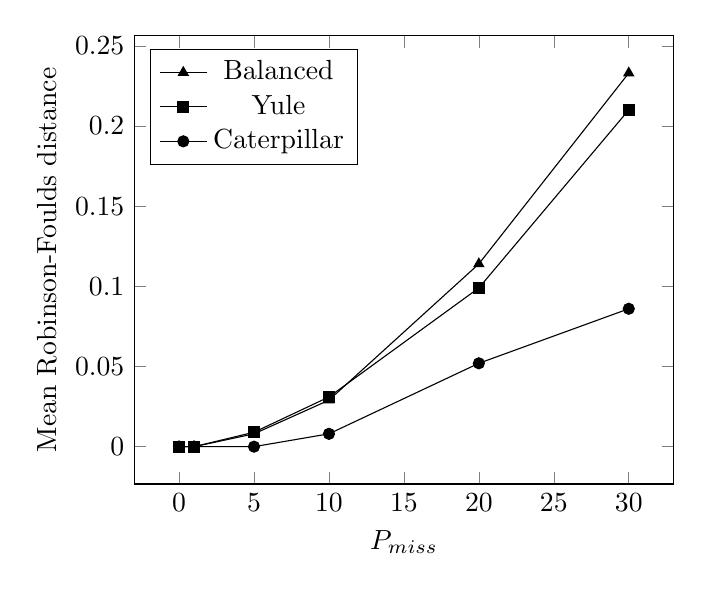
\begin{tikzpicture}
            \begin{axis}[xlabel=$P_{miss}$,
          ylabel=Mean Robinson-Foulds distance,
          yticklabels={,0,0.05,0.1,0.15,0.2,0.25},
          legend pos=north west]
      \addplot[color=black,mark=triangle*] table[x=missing,y=mean]{
missing  mean      min      max     minc     maxc
0.0    0.000    0.000    0.000       64       64
1.0    0.000    0.000    0.000       64       64
5.0    0.008    0.000    0.175       62       64
10.0    0.029    0.000    0.238       61       64
20.0    0.114    0.000    0.635       31       64
30.0    0.233    0.000    0.698       30       64
      };
      \addlegendentry{Balanced}
      \addplot[color=black,mark=square*] table[x=missing,y=mean]{
missing  mean      min      max     minc     maxc
0.0    0.000    0.000    0.000       64       64
1.0    0.000    0.000    0.000       64       64
5.0    0.009    0.000    0.206       62       64
10.0    0.031    0.000    0.397       49       64
20.0    0.099    0.000    0.619       29       64
30.0    0.210    0.000    0.857       14       64
      };
      \addlegendentry{Yule}
      \addplot[color=black,mark=*] table[x=missing,y=mean]{
missing  mean      min      max     minc     maxc
0.0    0.000    0.000    0.000       64       64
1.0    0.000    0.000    0.000       64       64
5.0    0.000    0.000    0.000       64       64
10.0    0.008    0.000    1.000       63       64
20.0    0.052    0.000    1.000       62       64
30.0    0.086    0.000    1.000       62       64
      };
      \addlegendentry{Caterpillar}
    \end{axis}

  \end{tikzpicture}
  \endpgfgraphicnamed  
  \caption{For all three equidistant $X$-tree types, we plot the normalised
    Robinson-Foulds distance between $T$ and $T'|_Y$.}
  \label{fig:rob-foulds-shapes}
\end{figure}

\begin{figure}
  \centering
  \beginpgfgraphicnamed{simulation-nleaves}
  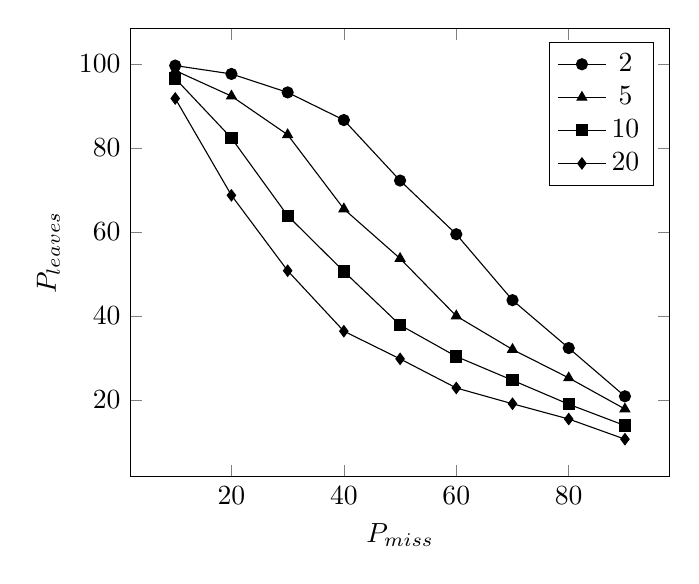
\begin{tikzpicture}
        \begin{axis}[ xlabel=$P_{miss}$,
      ylabel=$P_{leaves}$,
      legend pos=north east]

      \addplot[color=black,mark=*] table[x=mcords,y=nleaves] {
 mcords  nleaves   ncords
  10.00    99.64    99.53
  20.00    97.65    94.95
  30.00    93.25    88.97
  40.00    86.67    77.56
  50.00    72.26    56.96
  60.00    59.48    39.49
  70.00    43.78    22.29
  80.00    32.38    12.63
  90.00    20.89     6.47
   };
   \addlegendentry{2}
      \addplot[color=black,mark=triangle*] table[x=mcords,y=nleaves] {
 mcords  nleaves   ncords
  10.00    98.46    96.99
  20.00    92.37    86.98
  30.00    83.17    71.69
  40.00    65.50    47.52
  50.00    53.70    32.66
  60.00    40.01    18.88
  70.00    32.04    12.24
  80.00    25.27     8.50
  90.00    17.86     5.54
   };
   \addlegendentry{5}
      \addplot[mark=square*,color=black] table[x=mcords,y=nleaves] {
 mcords  nleaves   ncords
  10.00    96.57    93.85
  20.00    82.38    71.98
  30.00    63.89    46.22
  40.00    50.62    30.73
  50.00    37.86    17.49
  60.00    30.37    11.50
  70.00    24.71     7.92
  80.00    19.00     5.27
  90.00    13.92     3.85
   };
   \addlegendentry{10}
      \addplot[color=black,mark=diamond*] table[x=mcords,y=nleaves] {
 mcords  nleaves   ncords
  10.00    91.81    86.00
  20.00    68.75    53.41
  30.00    50.79    30.61
  40.00    36.39    17.35
  50.00    29.80    11.57
  60.00    22.87     7.10
  70.00    19.11     5.28
  80.00    15.48     3.87
  90.00    10.68     2.70
   };
   \addlegendentry{20}
    \end{axis}

  \end{tikzpicture}
  \endpgfgraphicnamed  
  \caption{For $T'$ an $X$-tree with $|X|=100$ and maximum out-degree $k= 2$,
    $5$, $10$ and $20$ we depict the proportion of $X$ which forms the leaf
    set of $T$. -- see text for details.  }
  \label{fig:simulation-nleaves}
\end{figure}

We observed that, independent of the type of equidistant tree considered, the
Robinson-Foulds distance between $T'|_Y$ and $T$ increases as the number of
distance values decreases, which is as expected. Having said that, out of all
three $X$-tree types equidistant caterpillar trees were reconstructed most
accurately with a mean normalised Robinson-Foulds distance below 0.1 even when
$30\%$ of the distance values were missing. A potential reason for this might
be that to correctly reconstruct a internal vertex $v$ of $T'$ the child-edge
graph associated to $v$ must be a complete graph (see
Section~\ref{sec:lassoing-rooted-x}).  In a caterpillar tree there is only one
cherry, all other internal vertices have a child that is a tree.  So the
likelihood that the child-edge graph associated to an internal vertex is a
complete graph is high as an edge in that vertex's child edge graph tends to
be supported by many leaf pairs of $T$ implying that \textsc{Lasso} correctly
reconstructs $v$. On the other hand, a balanced tree has the highest number of
cherries. Thus, the likelihood that the child-edge graph associated to such
vertices is not a complete graph increases as the number of missing distance
values grows, implying that $T$ may be very different from $T'|_Y$. Given that
it is well-known that trees generated under the Yule-Harding model tend to be
highly balanced (see e.\,g.\,\cite[Section 2.5]{semple2003phylogenetics}) it
is unsurprising to see that equidistant Yule-Harding trees and equidistant
balanced trees exhibit a similar behaviour.  Interestingly, equidistant
Yule-Harding trees were reconstructed slightly more accurately than
equidistant balanced trees overall, presumably due to small departures from a
purely balanced state.

\begin{algorithm}[h!]
  \caption{Random tree generation}
  \label{alg:random-tree}
  \textbf{Input:} A set $X$ and an integer $k$.
  
  \textbf{Output:} An equidistant $X$-tree with maximum
  out-degree $k$.

  \begin{itemize}
  \item[1.] Choose an integer 
$p$ in $\{2, \dotsc, \min(|X|,k)\}$ and some subset $C$ of $X$ of size $p$.
  \item[2.] Construct a tree $T$ with root $\rho_T$ by
attaching each element $c$ in $C$ via an edge to $\rho_T$ 
and setting the weight of that edge to $ 1+ \max_{x \in X} \, height(x)
- height(c)$.
  \item[3.] Put $X := (X - C) \cup \{\rho_T\}$.
  \item[4.] If $|X| > 1$ go to step 1, otherwise return $T$ 
%where $X = \{T\}$.
    and its edge-weighting.
  \end{itemize}
\end{algorithm}

Figure~\ref{fig:rob-foulds-shapes} suggests that for low quantities of missing
distances, \textsc{Lasso} is very good at exploiting redundancy in a given
distance matrix to correctly reconstruct the underlying equidistant $X$-tree,
independent of the tree type. To better understand how much this observation
is dependent on the fact that the starting $X$-trees were all binary, we also
investigated the influence of the maximal vertex degree $k$ of such a tree on
\textsc{Lasso}'s performance. To this end, we generated $500$ random
equidistant $X$-trees $(T',\omega')$ with maximum vertex out-degree $k$ as
described in Algorithm~\ref{alg:random-tree}.  The values for $k$ that we used
in this study were $k=2$, $5$, $10$, $20$ and the size of $X$ was always
$100$. We summarise our results in Figure~\ref{fig:simulation-nleaves} in
terms of the average percentage $P_{leaves}$ of the elements in $X$ that are
also present in the leaf set of the equidistant tree $(T,\omega)$ returned by
\textsc{Lasso}.

As expected, $P_{leaves}$ is very high (above $80\%$) for all values of $k$ if
the number of missing distances is not too large ($P_{miss}\leq 10\%$) which
is encouraging from a supertree perspective as the out-degree of a vertex can
be comparatively high in such trees.  However with an increasing number of
missing distances, equidistant $X$-trees with a lower maximal degree seem to
fare better overall. More precisely, in the case $k=2$ the equidistant tree
returned by \textsc{Lasso} still contains $80\%$ of the leaves of $T'$ even if
$40\%$ of the distance values are missing. To obtain a similar result for
$k=20$ only around $10\%$ of the distance values are allowed to be missing
from a distance matrix.  A potential reason for this discrepancy might be that
the more distances are missing from a distance matrix the more likely it is
for the child-edge graph of a high out-degree vertex not to be a complete
graph and thus to not be correctly reconstructed by \textsc{Lasso}.

\subsection{A yeast dataset}
\label{sec:yeast-dataset}

To test \textsc{Lasso} on a real biological dataset, again as a tree
reconstruction approach in the face of missing data, we applied it to a
distance matrix generated for the analysis of several intra-specific strains
of yeast.  In \cite{west14ribosomal} the authors identified both fully and
partially resolved single nucleotide polymorphisms (SNPs and pSNPS) within the
ribosomal DNA (rDNA) tandem arrays of 26 strains of the wild yeast
\textit{Saccharomyces paradoxus}.  A distance matrix was constructed from the
resulting allele frequency dataset using the Cavalli-Sforza and Edwards Chord
distance measure \cite{cavalli}.  A phylogenetic tree was estimated using
Neighbor Joining.  The tree was rooted by analysing rDNA variation in S288c,
the type strain of the closely related baker's yeast \textit{Saccharomyces
  cerevisiae}.  We note that the rooted tree built with either \textsc{UPGMA}
or \textsc{Lasso} is very similar to the authors' tree suggesting that the
tree underlying the dataset is indeed equidistant. From the distance $D$ on
the strains induced by the \textsc{Lasso}-tree we then randomly removed $10\%$
of the distance values ensuring that (i) whenever we removed for two strains
$x$ and $y$ the distance $D(x,y)$ we also removed the distance $D(y,x)$, that
(ii) values of the form $D(x,x)$ where $x$ denotes a strain did not count
towards the removed $10\%$, and that (iii) the graph $\Gamma(\cL_D)$ remained
connected. We present the equidistant tree returned by \textsc{Lasso} in
Figure~\ref{fig:yeast-tree-complete}.  Note that this tree contains all 26
input taxa. Furthermore, its topology is highly similar to that produced, on
the full distance matrix, by \cite{west14ribosomal}. Most importantly, the
groupings of the American, Far Eastern and European strains are preserved, as
is the separation of the UK and non-UK derived strains within the European
group. Furthermore, the putative European/Far Eastern hybrid strains $N\_17$
and $N\_45$ are located within the tree at positions consistent with such an
evolutionary history. While some minor changes in topology are seen within the
European and American groups, the relationships within the Far Eastern group
are wholly preserved once 10\% of distances have been removed.

\begin{figure}
  \centering
  \beginpgfgraphicnamed{yeast-tree-complete}
  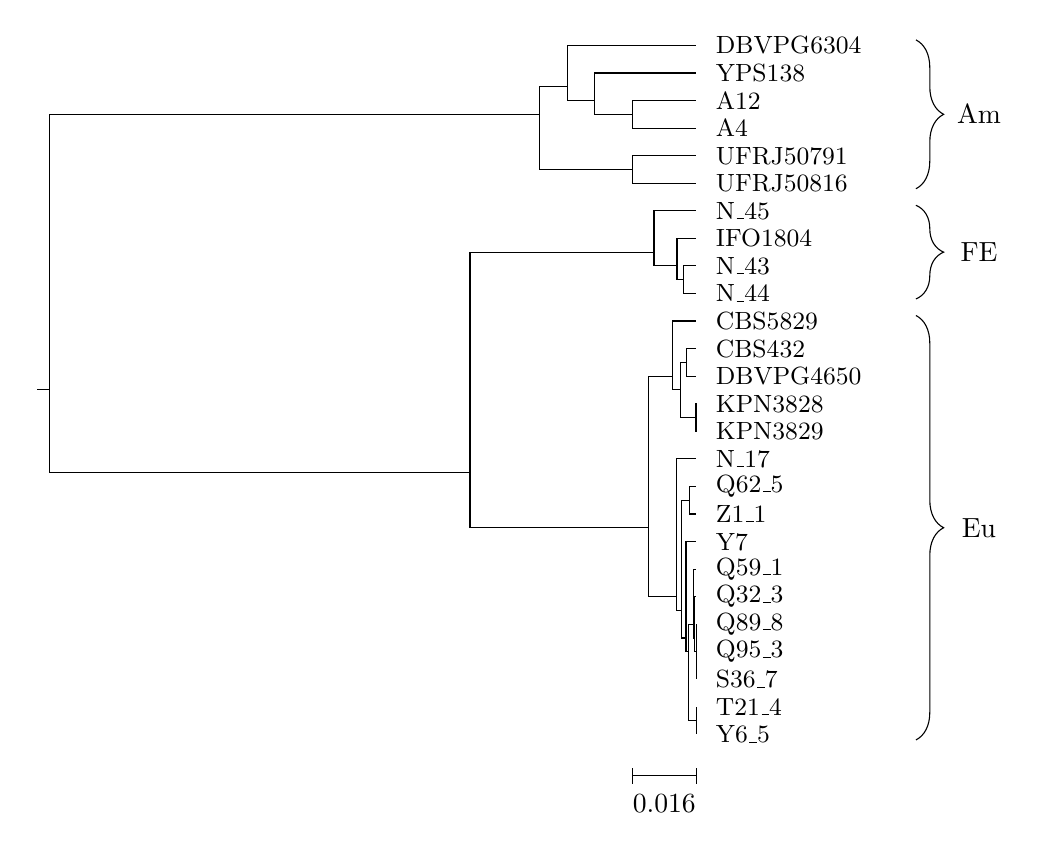
\begin{tikzpicture}[xscale=50,yscale=0.35]
    \node (r) at (0.0,0.0) {};
\node (rr) at (-0.0032859843,0.0) {};
\draw (r.center) -- (rr.center);
\node (r1) at (0.124339595,10.0) {};
\node (r11) at (0.1315726,11.0) {};
\node[label={[font=\small]right:DBVPG6304}] (r111) at (0.16429922,12.5) {};
\draw (r11.center) |- (r111.center);
\node (r112) at (0.13834648,10.5) {};
\node[label={[font=\small]right:YPS138}] (r1121) at (0.16429923,11.5) {};
\draw (r112.center) |- (r1121.center);
\node (r1122) at (0.14807872,10.0) {};
\node[label={[font=\small]right:A12}] (r11221) at (0.16429922,10.5) {};
\draw (r1122.center) |- (r11221.center);
\node[label={[font=\small]right:A4}] (r11222) at (0.16429922,9.5) {};
\draw (r1122.center) |- (r11222.center);
\draw (r112.center) |- (r1122.center);
\draw (r11.center) |- (r112.center);
\draw (r1.center) |- (r11.center);
\node (r12) at (0.14807872,8.0) {};
\node[label={[font=\small]right:UFRJ50791}] (r121) at (0.16429922,8.5) {};
\draw (r12.center) |- (r121.center);
\node[label={[font=\small]right:UFRJ50816}] (r122) at (0.16429922,7.5) {};
\draw (r12.center) |- (r122.center);
\draw (r1.center) |- (r12.center);
\draw (r.center) |- (r1.center);
\node (r2) at (0.106791504,-3.0) {};
\node (r21) at (0.15354072,5.0) {};
\node[label={[font=\small]right:N\_45}] (r211) at (0.16429922,6.5) {};
\draw (r21.center) |- (r211.center);
\node (r212) at (0.15938796,4.5) {};
\node[label={[font=\small]right:IFO1804}] (r2121) at (0.1642992,5.5) {};
\draw (r212.center) |- (r2121.center);
\node (r2122) at (0.16096471,4.0) {};
\node[label={[font=\small]right:N\_43}] (r21221) at (0.16429922,4.5) {};
\draw (r2122.center) |- (r21221.center);
\node[label={[font=\small]right:N\_44}] (r21222) at (0.16429922,3.5) {};
\draw (r2122.center) |- (r21222.center);
\draw (r212.center) |- (r2122.center);
\draw (r21.center) |- (r212.center);
\draw (r2.center) |- (r21.center);
\node (r22) at (0.15209067,-5.0) {};
\node (r221) at (0.15820873,0.5) {};
\node[label={[font=\small]right:CBS5829}] (r2211) at (0.16429923,2.5) {};
\draw (r221.center) |- (r2211.center);
\node (r2212) at (0.16037111,0.0) {};
\node (r22121) at (0.16173123,1.0) {};
\node[label={[font=\small]right:CBS432}] (r221211) at (0.16429923,1.5) {};
\draw (r22121.center) |- (r221211.center);
\node[label={[font=\small]right:DBVPG4650}] (r221212) at (0.16429923,0.5) {};
\draw (r22121.center) |- (r221212.center);
\draw (r2212.center) |- (r22121.center);
\node (r22122) at (0.16422524,-1.0) {};
\node[label={[font=\small]right:KPN3828}] (r221221) at (0.16429923,-0.5) {};
\draw (r22122.center) |- (r221221.center);
\node[label={[font=\small]right:KPN3829}] (r221222) at (0.16429923,-1.5) {};
\draw (r22122.center) |- (r221222.center);
\draw (r2212.center) |- (r22122.center);
\draw (r221.center) |- (r2212.center);
\draw (r22.center) |- (r221.center);
\node (r222) at (0.15933868,-7.5) {};
\node[label={[font=\small]right:N\_17}] (r2221) at (0.16429923,-2.5) {};
\draw (r222.center) |- (r2221.center);
\node (r2222) at (0.16052471,-8.0) {};
\node (r22221) at (0.16261172,-4.0) {};
\node[label={[font=\small]right:Q62\_5}] (r222211) at (0.16429922,-3.5) {};
\draw (r22221.center) |- (r222211.center);
\node[label={[font=\small]right:Z1\_1}] (r222212) at (0.16429922,-4.5) {};
\draw (r22221.center) |- (r222212.center);
\draw (r2222.center) |- (r22221.center);
\node (r22222) at (0.1616616,-9.0) {};
\node[label={[font=\small]right:Y7}] (r222221) at (0.16429922,-5.5) {};
\draw (r22222.center) |- (r222221.center);
\node (r222222) at (0.16238672,-9.5) {};
\node (r2222221) at (0.16348071,-8.5) {};
\node[label={[font=\small]right:Q59\_1}] (r22222211) at (0.16429922,-6.5) {};
\draw (r2222221.center) |- (r22222211.center);
\node (r22222212) at (0.16382422,-9.0) {};
\node[label={[font=\small]right:Q32\_3}] (r222222121) at (0.16429922,-7.5) {};
\draw (r22222212.center) |- (r222222121.center);
\node (r222222122) at (0.16429922,-9.5) {};
\node[label={[font=\small]right:Q89\_8}] (r2222221221) at (0.16429922,-8.5) {};
\draw (r222222122.center) |- (r2222221221.center);
\node[label={[font=\small]right:Q95\_3}] (r2222221222) at (0.16429922,-9.5) {};
\draw (r222222122.center) |- (r2222221222.center);
\node[label={[font=\small]right:S36\_7}] (r2222221223) at (0.16429922,-10.5) {};
\draw (r222222122.center) |- (r2222221223.center);
\draw (r22222212.center) |- (r222222122.center);
\draw (r2222221.center) |- (r22222212.center);
\draw (r222222.center) |- (r2222221.center);
\node (r2222222) at (0.16429922,-12.0) {};
\node[label={[font=\small]right:T21\_4}] (r22222221) at (0.16429922,-11.5) {};
\draw (r2222222.center) |- (r22222221.center);
\node[label={[font=\small]right:Y6\_5}] (r22222222) at (0.16429922,-12.5) {};
\draw (r2222222.center) |- (r22222222.center);
\draw (r222222.center) |- (r2222222.center);
\draw (r22222.center) |- (r222222.center);
\draw (r2222.center) |- (r22222.center);
\draw (r222.center) |- (r2222.center);
\draw (r22.center) |- (r222.center);
\draw (r2.center) |- (r22.center);
\draw (r.center) |- (r2.center);
\draw[|-|] (0.16429922,-14.0) -- (0.14786929,-14.0);
\node at (0.15608425,-15.0) {0.016};

\draw [decorate,decoration={brace,amplitude=10pt}]
(0.22, 12.7) -- (0.22, 7.3) node [black,midway,xshift=0.8cm] {Am};

\draw [decorate,decoration={brace,amplitude=10pt}]
(0.22, 6.7) -- (0.22, 3.3) node [black,midway,xshift=0.8cm] {FE};

\draw [decorate,decoration={brace,amplitude=10pt}]
(0.22, 2.7) -- (0.22, -12.7) node [black,midway,xshift=0.8cm] {Eu};

  \end{tikzpicture}
  \endpgfgraphicnamed
  \caption{An equidistant tree returned by \textsc{Lasso} from the yeast
    dataset with $10\%$ of the distances randomly removed. The sixteen
    European strains are denoted by the label ``Eu'', the four Far Eastern
    strains by ``FE'' and the six American strains by ``Am''. The uppermost
    five European strains (CBS5829 to KPN3829), together with N\_17, derive
    from outside the UK, with the remaining ten European strains having been
    isolated within the UK.}
  \label{fig:yeast-tree-complete}
\end{figure}

Since \textsc{Lasso}'s ability to reconstruct an equidistant tree from a
partial distance depends on both which distances are missing and the random
decisions made by the algorithm to break ties, we also constructed a consensus
tree from the equidistant trees returned by \textsc{Lasso} (see
Fig.~\ref{fig:yeast-tree-consense}).  For this, we used an approach similar to
bootstrapping and indicate in terms of numbers assigned to each internal
vertex, except the root, how often each cluster induced by such a vertex is
displayed by an equidistant tree returned by \textsc{Lasso}.  More precisely
we generated 100 partial distances with $10\%$ of the distances removed at
random as described above.  We then ran \textsc{Lasso} on each partial
distance resulting in a total of $100$ equidistant trees each supported, on
average, by a strong lasso with 205 cords (out of the possible 293).  The
resulting trees were then used as input to the \textsc{Consense} program
\cite{felsenstein1993phylip} with default settings to build a consensus tree
using the ``majority rule (extended)" option. This tree is again highly
consistent with the full distance matrix tree, differing only from
Figure~\ref{fig:yeast-tree-complete} in the relationship between the three
European strains Q89\_8, Q95\_3 and S36\_7. Noticeably, the support for the
bifurcation of the latter two strains is the only one in
Figure~\ref{fig:yeast-tree-consense} less than 74.

\begin{figure}
  \centering
  \beginpgfgraphicnamed{yeast-tree-consense}
  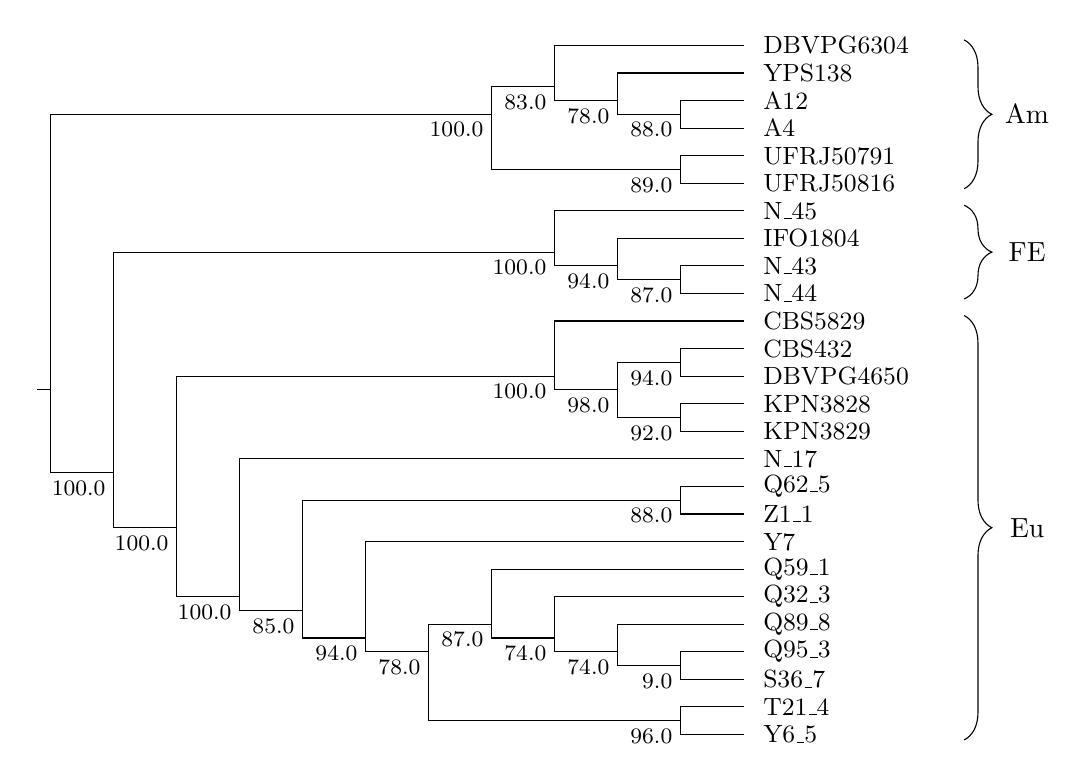
\begin{tikzpicture}[xscale=0.8,yscale=0.35]
    \node (r) at (0.0,0.0) {};
\node (rr) at (-0.22,0.0) {};
\draw (r.center) -- (rr.center);
\node[label={[label distance=-.2cm,font=\footnotesize]below left:100.0}] (r1) at (7.0,10.0) {};
\node[label={[label distance=-.2cm,font=\footnotesize]below left:83.0}] (r11) at (8.0,11.0) {};
\node[label={[font=\small]right:DBVPG6304}] (r111) at (11.0,12.5) {};
\draw (r11.center) |- (r111.center);
\node[label={[label distance=-.2cm,font=\footnotesize]below left:78.0}] (r112) at (9.0,10.5) {};
\node[label={[font=\small]right:YPS138}] (r1121) at (11.0,11.5) {};
\draw (r112.center) |- (r1121.center);
\node[label={[label distance=-.2cm,font=\footnotesize]below left:88.0}] (r1122) at (10.0,10.0) {};
\node[label={[font=\small]right:A12}] (r11221) at (11.0,10.5) {};
\draw (r1122.center) |- (r11221.center);
\node[label={[font=\small]right:A4}] (r11222) at (11.0,9.5) {};
\draw (r1122.center) |- (r11222.center);
\draw (r112.center) |- (r1122.center);
\draw (r11.center) |- (r112.center);
\draw (r1.center) |- (r11.center);
\node[label={[label distance=-.2cm,font=\footnotesize]below left:89.0}] (r12) at (10.0,8.0) {};
\node[label={[font=\small]right:UFRJ50791}] (r121) at (11.0,8.5) {};
\draw (r12.center) |- (r121.center);
\node[label={[font=\small]right:UFRJ50816}] (r122) at (11.0,7.5) {};
\draw (r12.center) |- (r122.center);
\draw (r1.center) |- (r12.center);
\draw (r.center) |- (r1.center);
\node[label={[label distance=-.2cm,font=\footnotesize]below left:100.0}] (r2) at (1.0,-3.0) {};
\node[label={[label distance=-.2cm,font=\footnotesize]below left:100.0}] (r21) at (8.0,5.0) {};
\node[label={[font=\small]right:N\_45}] (r211) at (11.0,6.5) {};
\draw (r21.center) |- (r211.center);
\node[label={[label distance=-.2cm,font=\footnotesize]below left:94.0}] (r212) at (9.0,4.5) {};
\node[label={[font=\small]right:IFO1804}] (r2121) at (11.0,5.5) {};
\draw (r212.center) |- (r2121.center);
\node[label={[label distance=-.2cm,font=\footnotesize]below left:87.0}] (r2122) at (10.0,4.0) {};
\node[label={[font=\small]right:N\_43}] (r21221) at (11.0,4.5) {};
\draw (r2122.center) |- (r21221.center);
\node[label={[font=\small]right:N\_44}] (r21222) at (11.0,3.5) {};
\draw (r2122.center) |- (r21222.center);
\draw (r212.center) |- (r2122.center);
\draw (r21.center) |- (r212.center);
\draw (r2.center) |- (r21.center);
\node[label={[label distance=-.2cm,font=\footnotesize]below left:100.0}] (r22) at (2.0,-5.0) {};
\node[label={[label distance=-.2cm,font=\footnotesize]below left:100.0}] (r221) at (8.0,0.5) {};
\node[label={[font=\small]right:CBS5829}] (r2211) at (11.0,2.5) {};
\draw (r221.center) |- (r2211.center);
\node[label={[label distance=-.2cm,font=\footnotesize]below left:98.0}] (r2212) at (9.0,0.0) {};
\node[label={[label distance=-.2cm,font=\footnotesize]below left:94.0}] (r22121) at (10.0,1.0) {};
\node[label={[font=\small]right:CBS432}] (r221211) at (11.0,1.5) {};
\draw (r22121.center) |- (r221211.center);
\node[label={[font=\small]right:DBVPG4650}] (r221212) at (11.0,0.5) {};
\draw (r22121.center) |- (r221212.center);
\draw (r2212.center) |- (r22121.center);
\node[label={[label distance=-.2cm,font=\footnotesize]below left:92.0}] (r22122) at (10.0,-1.0) {};
\node[label={[font=\small]right:KPN3828}] (r221221) at (11.0,-0.5) {};
\draw (r22122.center) |- (r221221.center);
\node[label={[font=\small]right:KPN3829}] (r221222) at (11.0,-1.5) {};
\draw (r22122.center) |- (r221222.center);
\draw (r2212.center) |- (r22122.center);
\draw (r221.center) |- (r2212.center);
\draw (r22.center) |- (r221.center);
\node[label={[label distance=-.2cm,font=\footnotesize]below left:100.0}] (r222) at (3.0,-7.5) {};
\node[label={[font=\small]right:N\_17}] (r2221) at (11.0,-2.5) {};
\draw (r222.center) |- (r2221.center);
\node[label={[label distance=-.2cm,font=\footnotesize]below left:85.0}] (r2222) at (4.0,-8.0) {};
\node[label={[label distance=-.2cm,font=\footnotesize]below left:88.0}] (r22221) at (10.0,-4.0) {};
\node[label={[font=\small]right:Q62\_5}] (r222211) at (11.0,-3.5) {};
\draw (r22221.center) |- (r222211.center);
\node[label={[font=\small]right:Z1\_1}] (r222212) at (11.0,-4.5) {};
\draw (r22221.center) |- (r222212.center);
\draw (r2222.center) |- (r22221.center);
\node[label={[label distance=-.2cm,font=\footnotesize]below left:94.0}] (r22222) at (5.0,-9.0) {};
\node[label={[font=\small]right:Y7}] (r222221) at (11.0,-5.5) {};
\draw (r22222.center) |- (r222221.center);
\node[label={[label distance=-.2cm,font=\footnotesize]below left:78.0}] (r222222) at (6.0,-9.5) {};
\node[label={[label distance=-.2cm,font=\footnotesize]below left:87.0}] (r2222221) at (7.0,-8.5) {};
\node[label={[font=\small]right:Q59\_1}] (r22222211) at (11.0,-6.5) {};
\draw (r2222221.center) |- (r22222211.center);
\node[label={[label distance=-.2cm,font=\footnotesize]below left:74.0}] (r22222212) at (8.0,-9.0) {};
\node[label={[font=\small]right:Q32\_3}] (r222222121) at (11.0,-7.5) {};
\draw (r22222212.center) |- (r222222121.center);
\node[label={[label distance=-.2cm,font=\footnotesize]below left:74.0}] (r222222122) at (9.0,-9.5) {};
\node[label={[font=\small]right:Q89\_8}] (r2222221221) at (11.0,-8.5) {};
\draw (r222222122.center) |- (r2222221221.center);
\node[label={[label distance=-.2cm,font=\footnotesize]below left:9.0}] (r2222221222) at (10.0,-10.0) {};
\node[label={[font=\small]right:Q95\_3}] (r22222212221) at (11.0,-9.5) {};
\draw (r2222221222.center) |- (r22222212221.center);
\node[label={[font=\small]right:S36\_7}] (r22222212222) at (11.0,-10.5) {};
\draw (r2222221222.center) |- (r22222212222.center);
\draw (r222222122.center) |- (r2222221222.center);
\draw (r22222212.center) |- (r222222122.center);
\draw (r2222221.center) |- (r22222212.center);
\draw (r222222.center) |- (r2222221.center);
\node[label={[label distance=-.2cm,font=\footnotesize]below left:96.0}] (r2222222) at (10.0,-12.0) {};
\node[label={[font=\small]right:T21\_4}] (r22222221) at (11.0,-11.5) {};
\draw (r2222222.center) |- (r22222221.center);
\node[label={[font=\small]right:Y6\_5}] (r22222222) at (11.0,-12.5) {};
\draw (r2222222.center) |- (r22222222.center);
\draw (r222222.center) |- (r2222222.center);
\draw (r22222.center) |- (r222222.center);
\draw (r2222.center) |- (r22222.center);
\draw (r222.center) |- (r2222.center);
\draw (r22.center) |- (r222.center);
\draw (r2.center) |- (r22.center);
\draw (r.center) |- (r2.center);

\draw [decorate,decoration={brace,amplitude=10pt}]
(14.5, 12.7) -- (14.5, 7.3) node [black,midway,xshift=0.8cm] {Am};

\draw [decorate,decoration={brace,amplitude=10pt}]
(14.5, 6.7) -- (14.5, 3.3) node [black,midway,xshift=0.8cm] {FE};

\draw [decorate,decoration={brace,amplitude=10pt}]
(14.5, 2.7) -- (14.5, -12.7) node [black,midway,xshift=0.8cm] {Eu};

  \end{tikzpicture}
  \endpgfgraphicnamed
  \caption{Consensus tree built from 100 runs of \textsc{Lasso} on matrices
    with 10\% of the distances randomly removed.  The number next to a vertex
    shows the number of times the cluster induced by that vertex appeared in
    the input of \textsc{Consense}. The length of an edge is of no relevance.}
  \label{fig:yeast-tree-consense}
\end{figure}

\subsection{A wheat dataset}
\label{sec:wheat-dataset}

Next, we analysed two partially overlapping wheat genetic marker datasets in
order to evaluate the potential of \textsc{Lasso} as a supertree approach. The
first dataset (which we will refer to as dataset $A$) consisted of 57 NBS
(Nucleotide Binding Site) markers scored over 411 accessions, a subset of a
dataset developed within the GEDIFLUX EU Framework V project \cite{gediflux}
to assess genetic diversity over time across four major crops, including
wheat. The second dataset (which we will refer to as dataset $B$) consisted of
71 NBS markers scored over 118 accessions, a subset of a study comparing
genetic diversity within and between winter wheat accessions from Turkey,
Kazakhstan and Europe \cite{muge}, the latter comprising a small group of the
GEDIFLUX wheat accessions. Consequently, the two datasets share a common set
of 26 European winter wheat accessions, comprising 6.3\% and 22.0\% of their
accessions respectively. We will refer to this shared dataset as dataset $C$.

\begin{figure}
  \centering
  \includegraphics[scale=1]{figures/lasso-construction/supp-gedi-groups.pdf}
  \caption{The \textsc{Lasso} tree for wheat dataset $A$.}
  \label{fig:lasso-wheat-a}
\end{figure}

\begin{figure}
  \centering
  \includegraphics[scale=0.8]{figures/lasso-construction/supp-muge-groups.pdf}
  \caption{The \textsc{Lasso} tree for wheat dataset $B$.}
  \label{fig:lasso-wheat-b}
\end{figure} 

Equidistant trees were estimated for datasets A and B separately, using the
Modified Rogers measure \cite{reif} to calculate a distance matrix, followed
by tree construction with \textsc{Lasso}. For convenience, we denote the two
distance matrices as $d_A$ and $d_B$, where the index indicates the dataset to
which they refer. The resulting equidistant trees were found to be supported
by 77,577 (out of 84,255) and 6,844 (out of 6,903) distances from $d_A$ and
$d_B$ respectively, and are shown in Figures~\ref{fig:lasso-wheat-a} and
\ref{fig:lasso-wheat-b}.  We assessed the individual \textsc{Lasso} trees
according to population group data for the two datasets. In the original
analysis of dataset $B$ \cite{muge}, the model-based clustering method
STRUCTURE \cite{structure} was carried out to estimate the number of founder
populations underlying the dataset and the genetic contribution of each
population to each accession. We coloured branches of the \textsc{Lasso} tree
in Figure~\ref{fig:lasso-wheat-b} such that the colour of each branch
corresponded to the main population group to which the relevant accession
belonged.  For dataset A, we conducted our own population structure analysis,
here using the ADMIXTURE method \cite{admixture} with default parameter
values.  ADMIXTURE uses an identical genetic model to STRUCTURE, but a
different computational approach to optimise population parameters, rendering
it considerably faster to run.  The \textsc{Lasso} tree for dataset $A$,
coloured according to these groups, is shown in
Figure~\ref{fig:lasso-wheat-a}. For both datasets, we see that accessions
belonging to the same population group are largely clustered within the
equidistant trees. The large sizes of the two Lassos (encompassing 92.1\% and
99.1\% of distances within $d_A$ and $d_B$ respectively), together with the
consistency of population grouping across the equidistant trees, strongly
suggest the suitability of the \textsc{Lasso} approach in determining the
genetic relationships between accessions within both of these
datasets. Furthermore, we note the previous use of the \textsc{UPGMA} method
to analyse NBS markers for wheat accessions \cite{mantovani06nbs}.

To obtain a (partial) distance $D$ on the combined dataset of $411+118-26=503$
accessions we proceeded as follows. If $x$ and $y$ are accessions such that
one of them is contained in dataset $A\backslash C$ and the other in $A$ then
we put $D(x,y)=d_A(x,y)$. Similarly, if one of them is contained in dataset
$B\backslash C$ and the other in $B$ then we put $D(x,y)=d_B(x,y)$. For the
remaining case that both accessions are contained in the overlap we took the
mean, that is, we put $D(x,y)=d_A(x,y)+d_B(x,y))/2$ where $x$ and $y$ are the
accessions under consideration.  To mitigate against the fact that for some
accessions in $C$ the distance values $d_A(x,y)$ and $d_B(x,y)$ correlate more
strongly than for others we used the ratio $d_A(x,y)/d_B(x,y)$ to identify
outliers, which we subsequently removed from the analysis. For this, we
employed the distribution of these ratios and defined a distance value to be
an outlier if it is more than one interquartile range above the upper quartile
or one interquartile range below the lower quartile.

\begin{figure}
  \centering \makebox[\textwidth][c]{\includegraphics[width=1.15\textwidth,
    trim = 20mm 65mm 20mm 55mm, clip]{figures/lasso-construction/bigtree.pdf}}
  \caption{The equidistant supertree built by \textsc{Lasso} for the two wheat
    datasets. Accessions from the GEDIFLUX dataset ($A$) are indicated by
    green branches, those from the Turkish dataset ($B$) by blue branches,
    with the 26 accessions found in both datasets ($C$) indicated by red
    branches. Note that the shared accessions are spread across the supertree
    and that the tree contains all 503 input taxa.}
  \label{fig:wheat-supertree}
\end{figure}

In total, the distance matrix representing $D$ contained 90,814 entries (where
we exclude entries of the form $D(x,x)$ and only count entries of the form
$D(x,y)$ and $D(y,x)$ once) which equates to $28.1\%$ of the $126,253$
potential distance values of a distance matrix on $503$ taxa missing.  We then
used this distance as input for \textsc{Lasso} to obtain a supertree $T$ on
the combined dataset. We depict that supertree in (Fig.~
\ref{fig:wheat-supertree}) and remark in passing that the tree contains all
503 input taxa and that the size of the strong lasso returned by
\textsc{Lasso} supporting $T$ is 89,642. Put differently, $T$ is the unique
equidistant tree that displays correctly 98.7\% of the 90,814 distance values
for $D$.

To better understand the relevance of the obtained supertree $T$ we tested it
with regards to consistency with the original distances on the two
datasets. In addition, we compared its topology against the supertree
generated by the modified \textsc{MinCutSupertree} approach
\cite{page02mincut}.  For the former, we performed Mantel tests between the
distance matrices derived from $d_A$ and $d_B$ and the distances displayed by
$T$.  The tests showed a positive correlation of $0.57$ and $0.47$,
respectively, with $p$-values for both being $0.0009990$. These results
indicate that $T$ displayed relationships between accessions within the two
datasets appropriately, including the overlapping accessions.

For the latter, we employed again the Robinson-Foulds distance. More
precisely, we used the equidistant trees $T_A$ and $T_B$ generated by
\textsc{Lasso} from the datasets $A$ and $B$, respectively, to generate a
supertree $S$ using the modified \textsc{MinCutSupertree} approach. This tree
we then restricted to each of the data sets $A$ and $B$ resulting in the trees
$S|_A$ and $S|_B$, respectively. Next, we restricted the topology $t$ of $T$
to the accessions in $A$ and in $B$, respectively, resulting in the trees
$t|_A$ and $t|_B$ (where the index indicates the data set). For these four
trees we computed the Robinson-Foulds distances between them and found that
$D_{RF}(T_A,S|_A)= 96>79= D_{RF}(T_A,t|_A)$ and that $D_{RF}(T_B,S|_B)=
384>322=D_{RF}(T_B,t|_B)$.  This suggests that the topology of the supertree
returned by \textsc{Lasso} is closer to that of the original trees on the two
datasets than the supertree constructed by the modified
\textsc{MinCutSupertree} approach, thus highlighting {\sc Lassos}'s potential
as a supertree method.

\section{Conclusion}
\label{sec:conclusion}

In this chapter, we have proposed the novel \textsc{Lasso} approach both for
distance-based phylogenetic tree reconstruction and supertree construction.
\textsc{Lasso} is similar in spirit to \textsc{UPGMA} but takes as input
partial distances (as opposed to the complete distances required by
\textsc{UPGMA}) and aims to reconstruct a unique (in a well-defined sense),
equidistant tree by exploiting redundancy in a given distance matrix rather
than trying to estimate missing distance values as do approaches such as
\cite{criscuolo2008fastnj}. Given that equidistant trees can be exploited as
starting trees within a search of tree space, for sophisticated phylogenetic
methods such as Maximum Likelihood and Bayesian Inference
\cite{burbrink09molecular,bouckaert14beast}, \textsc{Lasso} might provide a
quick and promising way to extend these methods to data sets for which only
partial distance information is available. Such datasets might arise when, for
example, confidence in a distance value is low resulting in an exclusion of
that distance (and thus the taxa involved) from an analysis, or when combining
disparate but overlapping datasets in a supertree context.

We assessed the performance of \textsc{Lasso} by means of artificial and real
biological data.  For the former we considered three different types of binary
equidistant trees and found that, independent of the tree type, \textsc{Lasso}
showed great promise when up to approximately $10\%$ of distance values were
missing.  For higher percentages of missing distance values we found that the
type of equidistant tree started to affect our ability to accurately
reconstruct it. More precisely, the equidistant caterpillar tree was recovered
most accurately under our simulation scenario and the equidistant balanced
tree the least accurately, with the equidistant Yule-Harding tree faring
slightly better than the balanced tree.  We also found that \textsc{Lasso}
showed great promise when the (unknown) equidistant tree underlying the given
partial distance did not possess vertices of too high a degree if a high
proportion of distance values were missing.  Put another way, even with $10\%$
of distance values missing for an underlying equidistant tree with vertices of
maximal out-degree $10$, \textsc{Lasso} was still able to return a tree on
more than $80\%$ of the original taxa.

We also assessed the performance of \textsc{Lasso} on two real biological
datasets. In the first of these studies, a yeast dataset originally developed
and analysed in \cite{west14ribosomal} was successfully reconstructed by
\textsc{Lasso}, even with 10\% of distance values removed at random. In the
second study, \textsc{Lasso} was used to construct a supertree of two
partially overlapping wheat NBS marker datasets \cite{gediflux,
  muge}. Subsequent statistical tests showed both that the \textsc{Lasso}
supertree successfully displayed relationships found with the two original
datasets and that it was more consistent with the two underlying trees than a
supertree constructed using the rival modified \textsc{MinCutSupertree}
approach. Collectively, these studies suggest that \textsc{Lasso} is
potentially a highly useful method for both tree reconstruction and supertree
construction on real datasets.

It is interesting to speculate that the strong performance of \textsc{Lasso}
in a supertree context owes part of its success to its ability to reject
shared distances that are not highly correlated. Indeed, when we repeated our
Mantel tests comparing the equidistant supertree derived from the full
combined dataset (that is, not rejecting any shared distance values) to the
two separate distance matrices (A and B), the correlations were found to be
0.47 ($p = 0.0009990$) for both datasets. Although this performance is almost
identical for dataset $B$, we see that removing certain shared distances leads
to a highly improved result for dataset $A$, which we earlier noted possessed
a lower proportion of distance values within the \textsc{Lasso}.  In future,
an investigation of methods to combine datasets for supertree construction
would be highly valuable, to see whether a further improvement could be
obtained.

Additional future work might include updating the distance in each repetition
step in a different way.  An alternative might be to simply throw out outliers
and remain much more tolerant to non-ultrametric input.  Although as we become
more tolerant to this we are less able to claim that we are satisfying the
consistency property.  We decided to only remove distances to avoid the
problems that come with introducing distances that exist with other methods
(as in Section~\ref{sec:constr-from-part}), but it might also be worth
considering introducing distances under certain circumstances.  For example,
we may consider adding one distance if it would allow us to grow our suitable
clique further.  Also it might be interesting to investigate the
\textsc{Lasso} approach in a {\em relaxed} molecular clock framework
\cite{drummond06relaxed}.

In summary, we propose the \textsc{Lasso} approach to become a new method
within the molecular phylogenetics toolkit. Given its demonstrated potential
both in tree reconstruction in the face of missing data, and in supertree
construction, we believe it can play an important role within a key project of
our generation, uncovering the Tree of Life.

\section{Acknowledgements}
\label{sec:acknowledgements}

For their assistance in the preparation of the paper underlining this chapter
the authors gratefully acknowledge Lesley Boyd and Muge Sayar-Turet for
providing a wheat dataset and Andrei-Alin Popescu for help with the ADMIXTURE
analysis and testing of software.

%%% Local Variables:
%%% TeX-master: "thesis"
%%% End:


\chapter{Distinguished minimal toplogical lassos}
\label{cha:dist-minim-topl}

A classical result in distance based tree-reconstruction characterizes 
when for a distance $D$ on some finite set $X$ there exist a  uniquely
determined dendrogram on $X$ (essentially a rooted tree $T=(V,E)$ with 
leaf set $X$ and no degree two vertices but possibly the root and an 
edge weighting $\omega:E\to \mathbb R_{\geq 0}$) such 
that the distance $D_{(T,\omega)}$
induced by $(T,\omega)$ on $X$ is $D$.  Moreover,
algorithms that quickly reconstruct 
 $(T,\omega)$ from $D$ in this case are known.
However in many 
areas where dendrograms are being constructed such as Computational Biology
not all distances on $X$ are always available implying that
 the sought after dendrogram 
need not be uniquely determined anymore by the available distances
with regards to topology of the underlying tree, edge-weighting, or both. 
To better understand the 
structural properties a set $\cL\subseteq {X\choose 2}$ has to 
satisfy to overcome this problem,
%that the distances on the leaf pairs in $\cL$ 
%do in fact uniquely determine the dendrogram 
%in question, 
various types of lassos have been introduced. 
Here, we focus on the question of when
a lasso  uniquely determines the topology of 
a dendrogram's underlying
 tree, that is, it is a topological lasso for that tree.
We show that any
set-inclusion minimal topological lasso for such a tree 
$T$ can be transformed into a 'distinguished' 
minimal topological lasso $\cL$ for $T$, that is, 
the graph $(X,\cL)$ is a claw-free block graph. Furthermore, we
characterize such lassos in terms of the novel concept
of a cluster marker map for $T$ and present results concerning 
the heritability of such lassos in the context of the subtree 
and supertree problems.

\section{Introduction}

In many topical studies in Computational Biology ranging from 
gene onthology via genome wide association studies in population genetics
to evolutionary genomics,
the following fundamental mathematical problem is encountered: 
Given a distance $D$
on some set $X$ of objects, find a dendrogram $\mathcal D$ on $X$ (essentially
a rooted tree $T=(V,E)$ with no degree two vertices but
possibly the root whose leaf 
set is $X$ together with an edge-weighting 
$\omega:E\to\mathbb R_{\geq 0}$
-- see Fig.~\ref{fig:block-graph-motivation}
for  examples) such that the distance induced by $\mathcal D$
on any two of its leaves $x$ and $y$ 
equals $D(x,y)$. In the ideal case that the distances between 
any two elements of $X$ are available, it is well-understood
when such a tree is uniquely determined by them and fast algorithms
for reconstructing it from them are known 
(see e.\,g.\,\cite[Chapter 9.2]{DHKMS11}
and \cite[Chapter 7.2]{semple2003phylogenetics}  where dendrograms 
are considered in the slightly more general forms of dated rooted $X$-trees
and equidistant representations of dissimilarities, respectively,
and \cite[Chapter 3]{BG91} 
as well as the references in all three of them for more on this).
 
The reality however tends to be different in many cases in that
distances between pairs of objects might be 
missing or are  not sufficiently reliable to warrant 
inclusion of that distance in 
an analysis -- see e.g. \cite{P04,SMS10,SS10} for more on this topic
in an evolutionary genomics context). 
 Exclusion of such a distance might therefore be tempting but is clearly not 
always desirable which raises 
interesting mathematical, statistical, and algorithmical questions
(see e.\,g.\,\cite{de1984ultrametric,farach1995robust,schader1992mvl} for a study concerning the latter
and \cite{farach1995robust,guenoche1999approximations,guenoche2004extension,makarenkov2001nouvelle} for results concerning its unrooted variant).
One of them is the focus of this paper: Calling 
any subset of a finite set $X$ of size two a {\em cord} of  $X$ 
then for what sets $\cL$ of cords of $X$ do we need to know the
distances so that both the topology of the underlying tree and the edge-weights
of the dendrogram on $X$ that induced the distances on the cords
in $\cL$ is uniquely determined by $\cL$?

To help illustrate the intricacies of this question which is concerned
with the structure of the set $\cL$ and not so much with 
the actual distances on the cords in $\cL$,
denote for any two distinct elements $a,b\in X$ the cord $\{a,b\}$
by $ab$. Consider the dendrogram $\mathcal D$ with leaf set
$X=\{a,\ldots, e\}$ depicted in
Fig.~\ref{fig:lasso-example}(i) and assume
 that the distances on the cords of $\cL=\{ac,de,bc,ce,cd\}$
are induced by $\mathcal D$ so, for example, the distance 
on the cord $ab$ 
%is the distance between $a$ and $b$ which 
is four. Then the dendrogram $\mathcal D'$
depicted in Fig.~\ref{fig:lasso-example}(ii) induces the
same distances on the cords in $\cL$ as $\mathcal D$
but the topologies of the underlying trees $T$ and $T'$
of $\mathcal D$ and $\mathcal D'$, respectively, 
are clearly not the same in the sense that there exists no
bijection from $V(T)$ to $V(T')$ that is the
identity on $\{a,\ldots, e\}$ and induces a  rooted graph 
isomorphism from  $T$ to $T'$.
Thus, $\cL$ does
not uniquely determine $T$ and thus also not $\mathcal D$. However
as can be quickly checked the situation changes if and only if
the cord $ab$ (or a subset of ${X\choose 2}$ containing that cord)
is added to $\cL$.  To make this more precise, 
let $\cL'$ denote the resulting set of cords on $X$
and let $\mathcal D_1$ denote a dendrogram on $X$ for which the
topology of the underlying tree 
is the same as that of $\mathcal D$. If $\mathcal D_2$ is a dendrogram
on $X$  such that the distances on the
cords in $\cL'$ induced by $\mathcal D_1$ and $\mathcal D_2$ coincide then,
as is easy to verify, the topologies of the 
underlying trees of $\mathcal D_1$ and $\mathcal D_2$,  
respectively, must be the same 
and so must be their edge-weightings. Thus, $\cL'$
uniquely determines $\mathcal D$. 

Although an intriguing question, apart  from some recent results in \cite{HP13},
not much is known about it (see \cite{DHS11} and \cite{HS13}
for some partial results in case the tree in question is unrooted).
By formalizing a dendrogram in terms of a certain  edge-weighted
$X$-tree (see the next section for a precise definition
of this concept as well as all the other concepts
mentioned below) and using the concept of a
topological lasso which was originally introduced 
for unrooted phylogenetic trees with leaf set $X$
in \cite{DHS11} 
and extended to $X$-trees in \cite {HP13}, we study this question in
the form of when a set of cords of $X$  is a topological
lasso for a given $X$-tree $T$. In the context of this,
we are particularly interested in (set-inclusion) minimal topological
lassos $\cL$ for $T$ for which $
\bigcup \cL:=\bigcup_{A\in\cL} A=X$ holds. 

For $T$ an $X$-tree, we show for any such minimal topological
lasso $\cL$ for $T$ that in case the graph $\Gamma(\cL)$ whose
vertex set is $X$ and any two distinct elements $x$ and $y$
in $X$ joined by an edge if $xy\in \cL$ -- see
Fig~\ref{fig:block-graph-motivation}(i) for an example of
that graph for $\cL=\{ab,cd,ef,ac,ce,ea\}$ -- is a block
graph then the blocks of $\Gamma(\cL)$ are in 
one-to-one correspondence with
the non-leaf vertices of $T$ (Corollary~\ref{cor:bijection}). 
Furthermore, we establish in Theorem~\ref{theo:transform}
that any minimal topological lasso $\cL$ for $T$ can be transformed
into a very special type of minimal topological lasso $\cL^*$
for $T$ in that $\Gamma(\cL^*)$
is a claw-free block graph where a graph is called
{\em claw-free} if it does not contain a {\em claw}, that is, 
the complete bipartite graph $K_{1,3}$ as an induced subgraph \cite{H72}.
%Calling a minimal topological
%lasso $\cL$ for $T$ {\em distinguished} if $\Gamma(\cL)$ 
%does not contain a {\em claw}, that is, the complete
%bipartite graph $K_{1,3}$, we show that every minimal
%topological lasso for $T$ can be transformed into
%a distinguished minimal topological lasso for $T$ via a 
%sequence of minimal topological lassos for $T$
%whose length is bounded by the number of 
%non-leaf vertices of $T$ 
%(Theorem~\ref{theo:transform}).
%Thus, to every minimal topological lasso we can associate
%a minimal topological lasso $\cL$ for which $\Gamma(\cL)$
%is a {\em claw-free} block graph, that is, a
%block graph that does not contain a claw. 
Claw-free graphs have been shown to enjoy numerous properties relating
them to, for example, perfect graphs, perfect matchings, 
and maximum independent sets
(see e.\,g.\,\cite{FFZ97} and \cite{CFHV12} for overviews).  
Furthermore, claw-free block graphs were related in
\cite{BL09} to $k$-leaf powers of trees and their spectrum
was studied in \cite{GS01, MSST06} (see also
\cite{BR13} for a more general study of the adjacency matrix
of such graphs). 
Calling a minimal topological lasso $\cL$ for $T$ {\em distinguished}
if $\Gamma(\cL)$ is a claw-free block graph,
we present in Theorem~\ref{theo:characterization}
a characterization of a distinguished
minimal topological lasso for $T$  in terms of the novel
concept of a cluster marker
map for $T$. In addition, we characterize when a
distinguished minimal topological lasso for $T$ 
gives rise to a distinguished minimal topological
lasso for a subtree of $T$ (Theorem~\ref{theo:subtree})
and also present a partial answer to the canonical
analogue of a question raised for supertrees of unrooted
phylogenetic trees in \cite{DHS11}.

%As it turns out, a $X$-tree cannot be uniquely
%reconstructed from a distinguished
%minimal topological lasso $\cL$ for it since there exist
%non-equivalent $X$-trees that are lassoed by the same set of
%cords -- see e.g. Fig.~\ref{fig:block-graph-motivation} for an 
%example. However the situation changes if the actual distances
%on the cords in $\cL$ are being used.
%We conclude with presenting such a construction. 

The paper is organized as follows. In Section~\ref{sec:terminology},
we introduce relevant terminology surrounding $X$-trees and
lassos. In Section~\ref{sec:gamma-l-graph}, we 
collect first properties of the graph $\Gamma(\cL)$ associated
to a topological lasso $\cL$ and in Section~\ref{sec:blockgraph}, we 
establish Corollary~\ref{cor:bijection}. In Section~\ref{sec:distinguished}, 
we commence our study of distinguished minimal topological
and establish Theorem~\ref{theo:transform}. In Section~\ref{sec:sufficient},
we present a sufficient condition for when a 
minimal topological lasso is distinguished 
(Theorem~\ref{theo: distinguished-lasso-verification}) and in
Section~\ref{sec:characterization-distinguished}, we 
prove Theorem~\ref{theo:characterization}. We conclude with
Section~\ref{sec:subtree} where we establish Theorem~\ref{theo:subtree}
and also outline directions for further research.
%We conclude with Section~\ref{sec:reconstruction}
%where we present an algorithm for reconstructing
%an $X$-tree $T$ from the distances on the elements of the
%cords of a distinguished minimal topological lasso for
%$T$.


\section{Basic terminology and assumptions}\label{sec:terminology}
In this section, we introduce some relevant 
basic terminology surrounding $X$-trees,
their edge-weighted counterparts, and lassos.  Assume throughout the paper  
that $X$ is a finite set with at least 3 elements and that, unless
stated otherwise, all sets $\cL$ of
cords of $X$ considered in this paper 
satisfy the property  that
 %We call a subset $\cL\subseteq {X\choose 2}$ of $X$ a
%{\em covering} of $X$ is 
$X=\bigcup \cL$. 


\subsection{$X$-trees}
A {\em rooted tree} $T$ is a tree with a unique distinguished vertex 
called the
{\em root} of $T$, denoted by $\rho_T$. Throughout the paper, we 
assume that the degree of the root of a rooted tree is at least two.
A {\em rooted phylogenetic $X$-tree}, or {\em $X$-tree} for short, 
is a rooted tree $T=(V,E)$ with no degree two vertices but
possibly the root $\rho_T$ whose leaf set is $X$. We call 
an $X$-tree $T$ a {\em star-tree
on $X$} if every leaf of $T$ is adjacent with the root  of $T$ 
%and refer to an $X$-tree that is not the star-tree on $X$
%as a {\em non-degenerate} $X$-tree.

Suppose for the following  that
$T$ is an $X$-tree. Then we call a vertex of $T$ that is not
 a leaf of $T$ an {\em interior vertex}
of $T$ and denote the set of interior vertices of $T$ by $\iV(T)$.
We call an edge of $T$  that is incident with a leaf of $T$ a {\em pendant
edge} of $T$ and every edge of $T$ that is not a pendant edge
an {\em interior edge} of $T$.
Extending some of the terminology for directed graphs
to $X$-trees, we call for all vertices $v\in V(T)-\{\rho_T\}$
 an edge $e\in E(T)$
a  {\em parent edge of $v$} if $e$ is incident with $v$ and 
lies on the path from 
the root $\rho_T$ of $T$ to $v$. We refer to the vertex incident with $e$ 
 but distinct from $v$ as a {\em parent} of $v$.
 
Suppose for the following
that $v$ is an interior vertex of $T$. If $v$ is not the root of $T$
then we call an edge $e\in E(T)$ a {\em child edge of $v$} if $e$ is
incident with $v$ but is not crossed by the path from $\rho_T$ to $v$.  
In addition, we
call every edge incident with $\rho_T$ a {\em child edge of $\rho_T$}.
We call the vertex incident with a child edge of an
 interior vertex $w$ of $T$
 but distinct from $w$ a {\em child of $w$} and denote
 the set of all children of $v$ by $ch_T(v)$.
% and put $deg^+(w)=|ch_T(v)|$. 
 %If $deg^+(w)=2$ holds for all vertices 
 % If $|ch_T(w)|=2$ holds for all vertices 
% $w\in \iV(T)$ then we call $T$ {\em binary}. 
We call a vertex $w\in V(T)$ distinct from $v$
a {\em descendant} of $v$ if either $w$ is a child of $v$ or
there exists a path from $v$ to $w$ that crosses a child of $v$.
We denote the set of leaves 
of $T$ that are also descendants of $v$ by $L_T(v)$. If $v$ is a leaf
of $T$ then we put $L_T(v):=\{v\}$. If there
is no ambiguity as to which $X$-tree $T$ we are referring to then,
for all $v\in V(T)$,  we will write $L(v)$ rather than $L_T(v)$
and $ch(v)$ rather than $ch_T(v)$.  

We call a non-empty subset $L\subsetneq X$ of 
leaves of $T$ such that $L=L(v)$ holds for some
$v\in \iV(T)$ a {\em pseudo-cherry} of $T$. In that case,
we also call $v$ the {\em parent} of that pseudo-cherry. 
%If $\{x_1,\ldots, x_k\}$, $k\geq 2$, is a pseudo-cherry of
%some $X$-tree $T$ then we will sometimes write $x_1,\ldots, x_k$
%rather than $\{x_1,\ldots, x_k\}$.  
Note that every 
$X$-tree on three or more leaves must
contain at least one pseudo-cherry. Also note
that a pseudo-cherry of size two is 
a {\em cherry} in the usual sense (see e.g. \cite{semple2003phylogenetics}).
%In the special
%case that $|X|=3$, say $X=\{a,b,c\}$, and that $T$ has a cherry
%$a,b$, say,
%we call $T$ a {\em (rooted) triplet} and denote $T$ by $ab|c$ (or,
%equivalently, $c|ab$). 

For $x$ and $y$  distinct elements in $X$,
we call the unique vertex of $T$ that simultaneously lies on
the path from $x$ to $y$, on the path from $x$ to $\rho_T$, and
on the path from $y$ to $\rho_T$ the {\em last common ancestor of
$x$ and $y$}, denoted by $lca_T(x,y)$. More generally, for any 
subset $Y\subseteq X$ of size three or more,
we denote the subtree of $T$ with leaf set $Y$ and
vertices of degree two suppressed (except possibly the root)
by $T|_Y$ and call the root of $T|_Y$ the {\em last common ancestor of
$Y$}, denoted by $lca_T(Y)$.

Finally, suppose that $T'$ is be a further
$X$-tree. Then we say that $T$ and $T'$ 
are {\em equivalent} if there exists a bijection $\phi:V(T)\to V(T')$
that extends to a graph isomorphism between $T$ and $T'$ that is
the identity on $X$ and maps the root $\rho_T$ of $T$ to the
root $\rho_{T'}$ of $T'$. 
%We say that 
%$T'$ {\em refines} $T$ if, up to equivalence,
%$T$ can be obtained from $T'$ by collapsing edges of $T'$
%(see e.\,g.\, \cite{semple2003phylogenetics}). In that case, we will also refer to
%$T'$ as a {\em refinement} of $T$. 


\subsection{Edge-weighted $X$-trees and lassos}

Suppose for the following again that $T$ is an $X$-tree.
An {\em edge weighting $\omega$ of $T$} is a map
$\omega :E(T)\to \mathbb R_{\geq 0}$ that maps every
edge of $T$ to a non-negative real. Suppose that $\omega$
is an edge-weighting for $T$. Then
we call the pair $(T,\omega)$ an {\em edge-weighted} $X$-tree and $\omega$
{\em proper} if $\omega(e)>0$ holds for every interior edge
$e$ of $T$. We denote the distance induced by $(T,\omega)$
on the leaves of $T$ by $D_{(T,\omega)}$
and call $\omega$ {\em equidistant} if 
\begin{enumerate}
\item[(i)] $D_{(T,\omega)}(x,\rho_T)=  D_{(T,\omega)}(y,\rho_T)$, for all
$x,y\in X$, and
\item[(ii)] $D_{(T,\omega)}(x,u)\geq  D_{(T,\omega)}(x,v)$, for all
$x\in X$ and all $u,v\in V$ such that $u$ is encountered
before $v$ on the path from $\rho_T$ to $x$.
\end{enumerate} 

Suppose $\cL$ is a set of cords of $X$. Then  
we call two edge-weighted $X$-trees 
$(T_1,\omega_1)$ and $(T_2,\omega_2)$  {\em $\cL$-isometric} if 
$D_{(T_1,\omega_1)}(x,y)=D_{(T_2,\omega_2)}(x,y)$ 
holds for all cords $xy\in \cL$. We say that $\cL$ is
a  {\em topological lasso} for $T$ if for every $X$-tree $T'$ and
any equidistant, proper edge-weightings $\omega$ of $T$ and $\omega'$ of
$T$',  we have that $T$ and $T'$ are equivalent
whenever $(T,\omega)$ and  $(T',\omega')$ are $\cL$-isometric.
If $\cL$ is a topological lasso for $T$ then we also say that $T$ is 
{\em topologically lassoed} by $\cL$. Moreover, 
we say that $\cL$ is  a {\em (set-inclusion) minimal topological 
lasso for $T$} if 
$\cL$ is a topological lasso for $T$ but no cord $A\in \cL$
can be removed from $\cL$ such that $\cL-\{A\}$ is still a
topological lasso for $T$. 
For ease of readability, if the $X$-tree to which a
topological lasso $\cL$ refers is of no relevance
to the discussion, we will simply say that $\cL$ is a 
topological lasso. 

To illustrate some of these definitions, let $X=\{a,\ldots, f\}$ and
let $\cL$ be the set of cords such that $\Gamma(\cL)$ is the
graph depicted in Fig.~\ref{fig:block-graph-motivation}(i).
Using e.\,g.\,\cite[Theorem~7.1]{HP13} (see also 
Theorem~\ref{theo:characterization-topology} below)
it is easy to see that the $X$-trees depicted in
Fig.~\ref{fig:block-graph-motivation}(ii) and (iii) respectively
are topologically lassoed by $\cL$. In fact, $\cL$ is a minimal 
topological lasso for both of them.
\begin{figure}[h]
\begin{center}
\input{figures/dist-min-lass/lasso-2-trees.pdft}
\end{center}
\caption{\label{fig:block-graph-motivation}
(i) The graph $\Gamma(\cL)$ with vertex set $X=\{a,b,\ldots,f\}$
for the set $\cL=\{ab,cd,ef,ac,ce,ea\}$. (ii) and (iii)
Two non-equivalent $X$-trees $T$ and $T'$
that are both topologically lassoed by $\cL$. In fact, 
$\cL$ is a minimal topological lasso for either one of them.
}
\end{figure}


\section{The graphs $\Gamma(\cL)$ and 
$G(\cL,v)$}\label{sec:gamma-l-graph}


In this section, we investigate properties of the graph $\Gamma(\cL)$ 
associated to a %non-empty 
set $\cL$ of cords of $X$. We start by remarking  that
if there is no danger of confusion, we denote an edge 
$\{a,b\}$ of $\Gamma(\cL)$ by $ab$ rather than $\{a,b\}$.

To establish our first structural result 
for $\Gamma(\cL)$ (see 
Proposition~\ref{prop:gamma-l-connected}), 
we require further terminology. 
Suppose $T$ is an $X$-tree, $v\in \iV(T)$, and 
$\cL$ is a 
set of cords of $X$. Then we call
the graph $G_T(\cL,v)=(V_{T,v},E_{T,v})$ with vertex set $V_{T,v}$
the set of all child edges of $v$ and edge set $E_{T,v}$ the
set of all $\{e,e'\}\in {V_{T,v}\choose 2}$ for which there
exist leaves $a,b\in X$ such that
$e$ and $e'$ are edges on the path from $a$ to $b$ in $T$ 
and $ab\in \cL$ holds the {\em child-edge graph of $v$ (with respect 
to $T$ and $\cL$)}. Note that in case there is no danger of 
ambiguity with regards to the $X$-tree $T$ we are referring to, we
 will write $G(\cL,v)$ rather than $G_T(\cL,v)$ and $V_v$ and $E_v$
rather than $V_{T,v}$ and $E_{T,v}$. The next result which was originally
established in \cite[Theorem 7.1]{HP13}
states a a crucial property of child-edge graphs.

\begin{thm}\label{theo:characterization-topology}
Suppose $T$ is an $X$-tree and 
$\cL$ is a set of cords of $X$. 
Then the following are equivalent:
\begin{enumerate}
\item[(i)] $\cL$ is a topological lasso for $T$.
\item[(ii)] for every vertex $v\in \iV(T)$, the graph
$G(\cL,v)$ is a clique.
\end{enumerate}
\end{thm}



Denoting for an $X$-tree $T$, a topological lasso $\cL$ for
$T$, and an interior vertex $v\in \iV(T)$ 
the set of all cords $ab\in \cL$ for which
$v=lca_T(a,b)$ holds  by 
$\cA(v)$, Theorem~\ref{theo:characterization-topology}
readily implies $|\cA(v)|\geq {|ch(v)|\choose 2}$.
The next observation is almost trivial yet central to the paper and  
concerns the special case 
that $\cL$ is a minimal topological lasso for $T$. Its
proof which combines a straightforward counting argument 
with Theorem~\ref{theo:characterization-topology} is left to
the interested reader. To able to state it,
we denote for an interior vertex $v\in \iV(T)$ and a child edge $e\in E(T)$
of $v$  the child of $v$ indicent with $e$ by $v_e$.  

\begin{lem}\label{lem:size-A(v)}
Suppose $T$ is an $X$-tree and $\cL$ is a minimal topological 
lasso for $T$. Then, for all $v\in \iV(T)$, we have 
$|\cA(v)|={|ch(v)|\choose 2}$. In particular, for any two distinct child 
edges $e_1$ and 
$e_2$ of $v$ there exists precisely one pair 
$(a_1,a_2)\in L(v_{e_1})\times L(v_{e_2})$ such that 
$a_1a_2\in\cL$.
\end{lem}
%%%% the following proof is correct but commented out
%to shorten the paper 2013-04-29
%\begin{proof}
%Suppose for contradiction that there exist some $v\in \iV(T)$
%such that $|\cA(v)|> {deg^+(v)\choose 2}$. Then there exists
%an edge $e=\{e_1,e_2\}\in E_{T,v}$ and
%pairs $(a,b),(a',b')\in L(v_{e_1})\times L(v_{e_2})$
%such that  $ab,a'b'\in\cL$ and $|\{a_,b,a',b'\}|\geq 3$.
%Since $\cL$ is a minimal 
%topological lasso for $T$ and  so 
%$|\cL|=\sum_{w\in \iV(T)} {deg^+(v)\choose 2}$ is 
%implied by Theorem~\ref{theo:characterization-topology}, 
 %there must exist some vertex $w\in \iV(T)$ such that 
%$|\cA(w)|< {deg^+(v)\choose 2}$. But then $G(\cL,w)$ 
%is not a clique and so, in view of 
%Theorem~\ref{theo:characterization-topology}, 
% $\cL$ is not a topological lasso for $T$
%which is impossible.
%\epf
%\end{proof}

Note that Lemma~\ref{lem:size-A(v)} immediately implies that
any two minimal topological lassos for the same $X$-tree must
be of equal size. 

To be able to establish Proposition~\ref{prop:gamma-l-connected}, 
we require a further definition.
Suppose $T$ is an $X$-tree and $\cL$ is a topological 
lasso for $T$. Then for all $v\in V(T)$, we denote by $\Gamma_v(\cL)$
the subgraph of $\Gamma(\cL)$ induced by $L(v)$. Note that
in case $v$ is a leaf of $T$ and thus an element in $X$
the only vertex in $\Gamma_v(\cL)$ is $v$ (and 
$E(\Gamma_v(\cL))=\emptyset$).


\begin{pro}~\label{prop:gamma-l-connected}
Suppose $T$ is an $X$-tree and $\cL$ is a topological lasso for $T$. 
Then, for all $v\in V(T)$, the graph $\Gamma_v(\cL)$ is connected. 
In particular, 
$\Gamma(\cL)$ is connected.
\end{pro}
\begin{proof}
Assume for contradiction that there exists some vertex $v\in V(T)$
such that  $\Gamma_v(\cL)$ is not connected. Then $v$ cannot be
a leaf of $T$ and so $v\in \iV(T)$ must hold. Without loss of generality
we may assume that $v$ is such that for all descendants $w\in V(T)$ of $v$
the induced graph $\Gamma_w(\cL)$ is connected. Since $\cL$
is  a topological lasso for $T$ and so $G(\cL,v)$ is a clique,
it follows for any two distinct children $v_1,v_2\in ch(v)$  that 
there exists a pair $(x_1,x_2)\in L(v_1)\times L(v_2)$
such that $x_1x_2\in \cL$.  Since the assumption on $v$ implies 
that the graphs 
$\Gamma_{w}(\cL)$ are connected for all children $w\in ch(v)$,   
it follows that $\Gamma_v(\cL)$ is connected which is impossible.
Thus, $\Gamma_v(\cL)$ is connected, for all  $v\in V(T)$.
That $\Gamma(\cL)$ is connected is a trivial consequence.
\qquad
\end{proof}


\section{The case that $\Gamma(\cL)$ is a 
block graph}\label{sec:blockgraph}



To establish a further property of $\Gamma(\cL)$ 
which we will do in Proposition~\ref{prop:x-i-unique}, we require some
terminology related to block graphs (see e.\,g.\,\cite{diestel}). 
Suppose $G$ is a graph. Then a vertex of $G$ 
is called a {\em cut vertex} if its deletion (plus its
incident edges) disconnects $G$. A graph is called a {\em block} 
if it has at least one vertex, is connected, and does 
not contain a cut vertex. A {\em block of a graph $G$} is a maximal connected
subgraph of $G$ that is a block and a graph is called a {\em block graph}
if all of its blocks are cliques. For convenience, we refer to a
block graph with vertex set $X$ as a {\em block graph on X}.

As the example of the two minimal topological lassos 
$
%\cL=
\{ab,cd,ef,ac,ce,ea\}$ and $
%\cL'=
\{ab, bc,$  $cd, de, ef, fa\}$ 
for the $\{a,\ldots,f\}$-tree
depicted in Fig.~\ref{fig:block-graph-motivation}(ii)
indicates, the graph $\Gamma(\cL)$  associated to a
 minimal topological lasso  $\cL$
may be but need not be a block graph. 
However if it is
%$\cL$ is a minimal topological lasso for some $X$-tree 
%$T$ such that $\Gamma(\cL)$ is a block graph 
then Lemma~\ref{lem:size-A(v)}
can be strengthened to the following central result
where for all positive integers $n$ we 
put $\langle n\rangle :=\{1,\ldots, n\}$ and set
$\langle 0\rangle:=\emptyset$.

\begin{pro}\label{prop:x-i-unique}
Suppose $T$ is an $X$-tree and $\cL$ is a minimal topological 
lasso for $T$ such that $\Gamma(\cL)$ is a block graph.
Let $v\in \iV(T)$ and let $v_1,\ldots, v_l\in V(T)$ denote the
children of $v$ where
$l=|ch(v)|$.
Then, for all $i\in \langle l\rangle$, there exists a unique 
leaf $x_i\in L(v_i)$ such that $x_sx_t\in \cL$ holds for
all $s,t\in\langle l\rangle$ distinct.
\end{pro}
\begin{proof}
For all $v\in \iV(T)$ and all $w\in ch(v)$, put
$$
L^v_w:=\{x\in L(w): \mbox{ there exist } w'\in ch(v)-\{w\}
\mbox{ and } y\in L(w')
\mbox{ such that } xy\in \cL  \}.
$$
We need to show that $|L^v_w|=1$ holds for all $v\in \iV(T)$ 
and all $w\in ch(v)$. To see this,
note first that since $G(\cL,v)$ is a clique for all $v\in \iV(T)$, 
we have, for all $w\in ch(v)$ with $v\in \iV(T)$, that $L^v_w\not=\emptyset$. 
Thus,  $|L^v_w|\geq 1$ holds for all such $v$ and $w$.


To establish equality, suppose there exists some interior vertex  
$v\in \iV(T)$ and 
some child $v_1\in ch(v)$ such that $|L^v_{v_1}|\geq 2$.
Choose two distinct leaves $x_1$ and $y_1$ of $T$ 
contained in $L^v_{v_1}$
and denote the parent edge of $v_1$ by $e_1$. Note that $v_1=v_{e_1}$.
Since $y_1\in L^v_{v_1}$, there exists a child edge $e_2$ of $v$
distinct from $e_1$ and some $x_2\in L(v_{e_2})$ such that
$y_1x_2\in\cL$. In view of $x_1\in L^v_{v_1}$, we 
distinguish between the cases that
(i) $x_1z\not\in\cL$ holds for all 
$z\in L(v_{e_2})$ and (ii) 
there exists some $z\in L(v_{e_2})$ such that
$x_1z\in\cL$.

Assume first that Case~(i) holds.
Then since $x_1\in L^v_{v_1}$ there exists 
a further child edge $e_3$ of $v$
and some $y_3\in L(v_{e_3})$ such that $x_1y_3\in\cL$.
Since, by Theorem~\ref{theo:characterization-topology}, 
$G(\cL,v)$ is a clique and so $\{e_2,e_3\}$ is an edge 
in $G(\cL,v)$, there must exist leaves 
$y_2\in L(v_{e_2})$ and 
$x_3\in L(v_{e_3})$ such that 
$y_2x_3\in\cL$. By 
Proposition~\ref{prop:gamma-l-connected}, the graphs 
$\Gamma_{v_{e_i}}(\cL)$, $i=2,3$,
are connected and, by definition, clearly do not share a
vertex. Hence, there must exist a cycle  in $\Gamma(\cL)$ whose vertex
set contains $\bigcup_{j\in\langle 3\rangle} \{x_j,y_j\}$. But then
$x_1x_2\in \cL$ must hold since
 $\Gamma(\cL)$
is a block graph and so every block in $\Gamma(\cL)$ 
is a clique. By Lemma~\ref{lem:size-A(v)} 
applied to $e_1$ and $e_2$, it follows that $x_1=y_1$
as $x_1,y_1\in L(v_1)$ and $y_1x_2\in \cL$ which
is impossible.

Now assume that Case~(ii) holds, that is, there exists some
$z\in L(v_{e_2})$ such that $x_1z\in\cL$. Then 
Lemma~\ref{lem:size-A(v)} applied to $e_1$ and $e_2$
 implies $x_1=y_1$ as $y_1x_2\in\cL$ also holds which is impossible.
 \qquad
\end{proof}

To illustrate Proposition~\ref{prop:x-i-unique}, 
let $T$ be the $X$-tree depicted
in Fig.~\ref{fig:block-graph-motivation}(ii)
and let $\cL$ be the set of cords of $X$ whose $\Gamma(\cL)$ graph is
pictured in  Fig.~\ref{fig:block-graph-motivation}(i). 
Using the notation from Proposition~\ref{prop:x-i-unique} and
 labelling the children of the root of $T$
from left to right by $v_1$, $v_2$ and $v_3$ 
it is easy to see that  Proposition~\ref{prop:x-i-unique} holds for
$x_1=a$, $x_2=c$ and $x_3=e$. 

The next result is the main result of this section and
lies at the heart of Corollary~\ref{cor:bijection}
which provides for an $X$-tree $T$ and a minimal topological lasso
$\cL$ for $T$ such that $\Gamma(\cL)$ is a block graph
a close link between
the blocks of $\Gamma(\cL)$, the interior vertices of $T$ and, for all 
$v\in \iV(T)$, the child-edge graphs $G(\cL,v)$. To establish it, we denote 
for all $v\in V(T)-\{\rho_T\}$ the parent edge of $v$ by $e_v$ and
the set of blocks of
a graph $G$ by $Block(G)$.


\begin{thm}\label{theo:unique-block}
Suppose $T$ is an $X$-tree and $\cL$ is a minimal topological lasso for
$T$ such that $\Gamma(\cL)$ is a block graph. Then, for all $v\in \iV(T)$,
there exists a unique block $B\in Block(\Gamma(\cL))$ such that
$v=lca_T(V(B))$.
\end{thm}
\begin{proof}
We first show existence. Suppose $v\in \iV(T)$. Let
$v_1,\ldots,v_l\in V(T)$ denote the children of $v$  where $l=|ch(v)|$.
By Proposition~\ref{prop:x-i-unique}, there exists, for 
all $i\in\langle l\rangle$, a unique
leaf $x_i\in L(v_i)$ such that, for all  $s,t\in \langle l\rangle$ distinct,
we have $x_sx_t\in \cL$. Put $A=\{x_1,\ldots,x_l\}$.
Clearly, $v=lca_T(A)$ and the graph $G(v)$ with vertex set $A$ and
edge set $E=\{\{x,y\}\in {A\choose 2}: xy\in\cL\}$ is a clique.
Then since $\Gamma(\cL)$ is a block graph
there must exist a block $B\in Block(\Gamma(\cL))$ that contains
$G(v)$ as an induced subgraph.

We claim that the graphs $G(v)$ and $B$  are equal. 
In view of the facts that $A\subseteq V(B)$, the
 blocks in a bock graph are cliques, and $G(v)$
is a clique it suffices to show that
$V(B)\subseteq A$. Suppose for contradiction that
there exists some $y\in V(B)-A$. Note first that $yx\in \cL$
must hold for all $x\in A$.
Next note that $y$ cannot be a descendant of $v$
since otherwise there would exist some $i\in\langle l\rangle$ such 
that $y\in L(v_i)$. Choose some  $j\in \langle l\rangle-\{i\}$. Then
Lemma~\ref{lem:size-A(v)} applied to $e_{v_i}$ and $e_{v_j}$
%the respective parent edges of $v_i$ and  $v_j$
 implies $x_i=y$  as $yx_j,x_ix_j\in\cL$
 which is impossible.

Choose some $x\in A$ and put 
$w=lca_T(x,y)$. Then $v$ is a descendant of $w$ and $w=lca_T(x,y)$ 
holds for all $x\in A$. Let $w_1\in V(T)$ and $w_2\in \iV(T)$ 
denote two distinct children of $w$ such that $y\in L(w_1)$ 
and $x\in L(w_2)$. Then Lemma~\ref{lem:size-A(v)} applied 
to $e_{w_1}$ and $e_{w_2}$
%the respective parent edges of $w_1$ and $w_2$ 
implies $x_i=x_j$ for all $i,j\in\langle l\rangle$ distinct
since $yx\in\cL$ holds
for all $x\in A$ which is impossible.
Thus, $V(B)\subseteq A$, as required. This concludes the proof of
the existence part of the theorem.

We next show uniqueness. 
Suppose for contradiction that there exists
some $v\in \iV(T)$ and distinct blocks $B,B'\in Block(\Gamma(\cL))$
such that  $lca_T(B)=v=lca_T(B')$. 
%Without loss of generality
%we may assume that $v$ is minimal, that is, for all
%descendents $w\in \iV(T)$ of $v$ there exists a unique  block $B_w$
%in $\Gamma(\cL)$ such that $w=lca_T(B_w)$. 
Since every block of $\Gamma(\cL)$ contains at least two vertices
as $\Gamma(\cL)$ is connected and $|X|\geq 3$,
we may choose distinct vertices  $b_1,b_2\in V(B)$ and 
$b_1',b_2'\in V(B')$ such that 
$lca_T(b_1,b_2)=lca_T(B)=v=lca_T(B')=lca_T(b_1',b_2')$. 
Note that $b_1b_2$ and  $b_1'b_2' $ must be cords in $\cL$
as $B$ and $B'$ are cliques of $\Gamma(\cL)$. 
We distinguish between the
cases that (i) $\{b_1,b_2\}\cap\{b_1',b_2'\}=\emptyset $
and (ii) $\{b_1,b_2\}\cap\{b_1',b_2'\}\not=\emptyset $.

We first show that Case (i) cannot hold. Assume for contradiction that
Case (i) holds, that is, $\{b_1,b_2\}\cap\{b_1',b_2'\}=\emptyset $.
We claim that 
$lca_T(b_1,b_1')=v$. Assume for contradiction that 
$w:=lca_T(b_1,b_1')\not=v$. Let $v_1\in ch(v)$ 
such that $v_1$ lies on the path from $v$ to
$w$. If $v\not =lca_T(b_2,b_2')$
then there exists a descendant $w'\in V(T)$ of $v$ such
that $lca_T(b_2,b_2')=w'$. Let $v_2\in ch(v)$ 
such that $v_2$ that lies on the path from $v$ to $w'$. Then
Lemma~\ref{lem:size-A(v)} applied to $e_{v_1}$ and $e_{v_2}$
%the respective parent edges of $v_1$ and $v_2$ 
implies $b_1=b_1'$ and $b_2=b_2'$ as $b_1b_2,b_1'b_2'\in \cL$
which is impossible. Thus, $lca_T(b_2,b_2')=v$
must hold. Let $v_2,v_2'\in ch(v)$ such that $b_2\in L(v_2)$
and $b_2'\in L(v_2')$. 
%By Lemma~\ref{lem:size-A(v)} applied to 
%$e_{v_2}$ and $e_{v_2'}$
%the respective parent edges of $v_2$ and $v_2'$ 
%there must exists a pair $(c,c')\in L_T(v_2)\times L_T(v_2')$ 
%such that $cc'\in \cL$.
Then since $b_1,b_1'\in L(v_1)$ and $b_1b_2, b_1'b_2'\in \cL$, 
Proposition~\ref{prop:x-i-unique}
implies $b_1'=b_1$.
%, $b_2=c$, and that $c'=b_2'$. 
Consequently,
$\{b_1,b_2\}\cap\{b_1',b_2'\}\not=\emptyset $ which is impossible.
%
%$C$: $b_1,b_2=c,c'=b_2',b_1'=b_1$ is a cycle in $\Gamma(\cL)$
%and so there must exist a block $B$ of $\Gamma(\cL)$ that contains
%$C$. Since every block in a blockgraph is a clique it follows that
%$b_1b_2'\in\cL$. But $b_1'b_2'\in \cL$ holds too and so, 
%by Lemma~\ref{lem:size-A(v)}, we obtain that $b_1=b_1'$ which is impossible.
Thus, $lca_T(b_2,b_2')=v$
cannot hold and so 
$$
lca_T(b_1,b_1')=v,
$$ 
as claimed.
Swapping the roles of $b_1,b_1'$ and $b_2,b_2'$ in the previous
claim implies that 
 $v= lca_T(b_2,b_2')$ must hold, too. 
 For $i=1,2$ let $v_i,v_i'\in ch(v)$ 
such that $b_i\in L(v_i)$ and $b_i'\in L(v_i')$.
Then, by Lemma~\ref{lem:size-A(v)}, 
there exist pairs $(c,c')\in L(v_1)\times L(v_1')$ and 
$(d,d')\in L(v_2)\times L(v_2')$ such that $cc',dd'\in\cL$. 
Since $(b_1,b_2)\in L(v_1)\times L(v_2)$ and 
$(b_1',b_2')\in L(v_1')\times L(v_2')$ and $b_1b_2,b_1'b_2'\in\cL$,
 Proposition~\ref{prop:x-i-unique} implies 
that $c=b_1$, $b_2=d$, $d'=b_2'$ and $c'=b_1'$. But then
$C$: $c'=b_1',b_2'=d', d=b_2, b_1=c,c'$ is a cycle in $\Gamma(\cL)$.
Since $\Gamma(\cL)$ is a block graph it follows that there must exist
a block $B^C$ in $\Gamma(\cL)$ that contains $C$. 
Since $\{b_1,b_2\}\subseteq V(B^C)\cap V(B)$ and two distinct blocks of
a block graph can share at most one vertex it follows that $B^C$ and 
$B$ must coincide. Since $\{b_1',b_2'\}\subseteq V(B^C)\cap V(B')$
holds too,
similar arguments imply that $B^C$ must also coincide with $B'$.
Thus, $B$ and $B'$ must be equal which is impossible.
Hence Case~(i) cannot hold, as required.

Thus, Case (ii) must hold, that is,  
$\{b_1,b_2\}\cap\{b_1',b_2'\}\not=\emptyset $. Since any 
two distinct blocks in a block graph can share at most one vertex 
it follows that $|\{b_1,b_2\}\cap\{b_1',b_2'\}|=1$.
Without loss of generality we may assume that $b_1=b_1'$. 
We first claim that 
$$
lca_T(b_2,b_2')=v.
$$
Assume to the contrary that $lca_T(b_2,b_2')\not=v$. 
Then there exist distinct children $v_1,v_2 \in ch(v)$ 
such that $b_1\in L(v_1)$ and $b_2,b_2'\in L(v_2)$ hold. 
Since both $b_1b_2$ and
$b_1'b_2'=b_1b_2'$ are cords in $\cL$, Lemma~\ref{lem:size-A(v)}
applied to 
$e_{v_1}$ and $e_{v_2}$
%the respective parent edges of $v_1$ and $v_2$ 
implies $b_2'=b_2$. Hence, $|\{b_1,b_2\}\cap\{b_1',b_2'\}|=2$ which 
is impossible. Thus, $lca_T(b_2,b_2')=v$, as claimed.

Let $v_1,v_2,v_2'\in ch(v)$  such that
$b_1\in L(v_1)$, $b_2\in L(v_2)$, and $b_2'\in L(v_2')$. 
By Lemma~\ref{lem:size-A(v)}, there exist some
$(c,c')\in L(v_2)\times L(v_2')$ such that $cc'\in \cL$.
Since we also have $(b_1,b_2)\in L(v_1)\times L(v_2)$ with
$b_1b_2\in \cL$ holding and $(b_1,b_2')\in L(v_1)\times L(v_2')$ with
$b_2'b_1=b_2'b_1'\in \cL$ holding, Proposition~\ref{prop:x-i-unique}
implies that $b_2=c$ and $b_2'=c'$. Hence, $C$: $b_1=b_1',b_2'=c',
c=b_2,b_1$ is a cylce in $\Gamma(\cL)$ and so similar arguments
as in the corresponding subcase for Case (i) imply that 
%
%Hence, there must exist
%a block $B^*$ in $\Gamma(\cL)$ that contains $C$. 
%Since $\{b_1,b_2\}\subseteq V(B^*)\cap V(B)$ and two distinct block in
%a block graph can share at most one vertex it follows that $B^*$ and 
%$B$ must conincide. Since $\{b_1,b_2'\}\subseteq V(B^*)\cap V(B')$
%similar arguments imply that $B^*$ must also conincide with $B'$.
%Thus, 
%
$B$ and $B'$ must coincide which is impossible. Thus, 
$lca_T(b_2,b_2')=v$ cannot hold  which concludes the discussion
of Case (ii) and thus the proof of the uniqueness part of the theorem.
\qquad \end{proof}

In view of Theorem~\ref{theo:unique-block}, we denote for $T$ an $X$-tree,
 a minimal topological lasso $\cL$ for $T$ such that $\Gamma(\cL)$
is a block graph, and a vertex $v\in \iV(T)$ 
the unique block $B$ in $\Gamma(\cL)$ for which 
$v=lca_T(V(B))$ holds by 
$B_v^{\cL}$, or simply by
$B_v$ if the set $\cL$ of cords is clear from the context. 
Moreover, we denote for all 
$x\in L(v)$ the child of $v$ on the path from  $v$ to $x$ by $v_x$. 

\begin{cor}\label{cor:bijection}
Suppose $T$ is an $X$-tree and $\cL$ is a minimal topological lasso for
$T$ such that $\Gamma(\cL)$ is a block graph. Then the map
$$
\psi:\iV(T)\to Block(\Gamma(\cL)) : v\mapsto B_v
$$
is a bijection with inverse map $\psi^{-1}:Block(\Gamma(\cL))\to \iV(T)$: 
$B\mapsto lca_T(V(B))$. Moreover, the map
$$
\chi:Block(\Gamma(\cL)) \to \{G(\cL, v)\,:\, v\in \iV(T)\}
: B\mapsto G(\cL,\psi^{-1}(B))
$$
is bijective and,
 for all $B\in Block(\Gamma(\cL))$, the map
$$
\xi_B:V(B) \to V_{\psi^{-1}(B)} 
: x\mapsto e_{\psi^{-1}(B)_x}
$$ 
induces a graph isomorphism between $B$ and the child-edge
graph $G(\cL, \psi^{-1}(B))$.
\end{cor}
\begin{proof}
In view of Theorem~\ref{theo:unique-block}, the map $\psi$ is clearly
well-defined and injective. To see that $\psi$ is surjective
let $B\in Block(\Gamma(\cL))$ and put $v_B=lca_T(V(B))$. Clearly,
$v_B\in \iV(T)$. Since 
$B_{v_B}=\psi(v_B)$ is a block in $\Gamma(\cL)$ for which also
$v_B=lca_T(V(B_{v_B}))$
 holds, Theorem~\ref{theo:unique-block} 
 implies that $\psi(v_B)$ and $B$ must coincide.
Consequently, $\psi$ must also be surjective and thus bijective. That
the map $\psi^{-1}$ is as stated is trivial.
Combined with Theorem~\ref{theo:characterization-topology}, 
the bijectivity of the map $\psi$ implies in particular that, 
for all $B\in Block(\Gamma(\cL))$,
the map $\xi_B: V(B) \to V_{\psi^{-1}(B)}  $ 
from $V(B)$ to the vertex set $V_{\psi^{-1}(B)}  $
of the child-edge graph $G(\cL, \psi^{-1}(B))$ induces a graph
isomorphism between $B$ and $G(\cL, \psi^{-1}(B))$.

To see that the map $\chi$ is bijective 
note first that $\chi$ is well-defined
since $\psi^{-1}(B)\in \iV(T)$ holds 
for all blocks $B\in Block(\Gamma(\cL))$. To see that $\chi$ is
injective assume that there exist blocks $B_1,B_2\in Block(\Gamma(\cL))$
such that $\chi(B_1)=\chi(B_2)$ but $B_1$ and $B_2$ are distinct.
Then $\psi^{-1}(B_1)\not= \psi^{-1}(B_2)$ as $\psi$ is a bijection from
$\iV(T)$ to  $Block(\Gamma(\cL)) $.
Combined with the fact that, for all
$B\in Block(\Gamma(\cL))$, the map $\xi_B$  induces a graph
isomorphism between $B$ and $G(\cL, \psi^{-1}(B))$
it follows that 
$\chi(B_1)=G(\cL,\psi^{-1}(B_1))\not=G(\cL,\psi^{-1}(B_2))=\chi(B_2)$ 
which is impossible. Thus, $\chi$ must be injective. Combined with the
fact that
$|Blocks(\Gamma(\cL))|=|\iV(T)|=|\{G(\cL, v)\,:\, v\in \iV(T)\}|$
it follows that $\chi$ must also be surjective and thus bijective.
\qquad \end{proof}

%Note that Corollary~\ref{cor:bijection} immediatelly implies that
%the map 
%$\chi:Block(\Gamma(\cL)) \to\{G(\cL, v)\,:\, v\in \iV(T)\}$:
%$B\mapsto G(\cL, lca_T(V(B))$ is also bijective

\section{A special type of minimal 
topological lasso} \label{sec:distinguished}

Returning to the example depicted in Fig.~\ref{fig:block-graph-motivation},
it should be noted that, in addition to being a block graph,
 $\Gamma(\cL)$ enjoys a very special
property where $\cL$ is the minimal topological lasso considered in
that example. More precisely, every vertex of $\Gamma(\cL)$
is contained in at most two blocks. 
Put differently, $\Gamma(\cL)$ is a claw-free graph. Motivated by this, we
call a minimal topological lasso $\cL$ {\em distinguished} if
$\Gamma(\cL)$ is a claw-free block graph.  Note that such
block graphs are precisely the
{\em line graphs of (unrooted) trees} where for any graph $G$ the
associated line graph has vertex set $E(G)$ and two vertices
$a,b\in E(G)$ are joined by an edge if $a\cap b\not=\emptyset$ \cite{H72}.  

In this section, we show in Theorem~\ref{theo:transform}
that distinguished minimal topological 
lassos are a very special type of lasso in that for
every $X$-tree $T$ any minimal topological lasso $\cL$ for $T$
can be transformed into a distinguished
minimal topological lasso 
$\cL^*$ for $T$ via a {\em repeated
application} (i.\,e.\,$l\geq 0$ applications) of the rule: 

\begin{enumerate}
\item[(R)] If $xy,yz\in \cL$ and $lca_T(y,z)$ is a descendant of  
$lca_T(x,y)$ in $T$ then delete $xy$ from the edge set of $\Gamma(\cL)$
and add the edge $xz$ to it. 
\end{enumerate}

Before we make this more precise which we will do next, we remark 
that since a topological lasso for a star tree
is in particular a distinguished minimal topological
lasso for it,  we will for this and the next two sections 
restrict our attention to {\em non-degenerate} $X$-trees,
that is, $X$-trees that are not star trees on $X$.

Suppose $T$ is a non-degenerate $X$-tree and $\cL$
is a set of cords of $X$. Let $\iV(T)$ denote
a set of colors and let 
$$
\gamma_{(\cL,T)}:\cL\to \iV(T):\, ab\mapsto lca_T(a,b)
$$
denote an edge coloring of $\Gamma(\cL)$
in terms of the interior vertices of $T$. Note that
if $\cL$ is a topological lasso for $T$
then Theorem~\ref{theo:characterization-topology} implies that
$\gamma_{(\cL,T)}$ is surjective. Returning to Rule (R),
note that a repeated application of that rule to such a set $\cL$ of cords
results in a  set $\cL'$ of cords that is also a 
topological lasso for $T$. Furthermore, note that if $\cL$ is a minimal
topological lasso for $T$ then $\cL'$ is necessarily also a minimal 
topological lasso for $T$. Finally note for all $v\in \iV(T)$ that
$|\gamma_{(\cL,T)}^{-1}(v)|=1$ or  
$|\gamma_{(\cL,T)}^{-1}(v)|\geq 3$ must hold in this case.


\begin{lem}\label{lem:3-edges-cycle}
Suppose $T$ is a non-degenerate $X$-tree and $\cL$ is a minimal
topological lasso for $T$.  Put $\gamma=\gamma_{(\cL,T)}$ and assume that
$v\in \iV(T)$ such that $|\gamma^{-1}(v)|\geq 3 $. Then for any three
pairwise distinct cords $c_1,c_2,c_3\in \gamma^{-1}(v)$, 
there exists a 
%(not necessarily induced)
cycle $C_v$ in $\Gamma(\cL)$ such that $c_1,c_2,c_3\in E(C_v)$ and,  
for all $c\in E(C_v)$,
$\gamma(c)$ either equals $v$ or is a descendant of $v$. 
\end{lem}
\begin{proof}
Let $v\in \iV(T)$ and let $c_1=x_1y_1$, $c_2=x_2y_2$ and
$c_3=x_3y_3$ denote three pairwise distinct cords in $\gamma^{-1}(v)$. 
For all $i\in\langle 3\rangle$,
let $v_i\in ch(v) $ such that $v_i$ lies on the path from $v$ to $x_i$ in $T$
and let $w_i\in ch(v)$ such that $w_i$ lies on the path from $v$ to
 $y_i$ in $T$.
Then, by Lemma~\ref{lem:size-A(v)},  there exists unique pairs
$(s_1,t_1)\in L(v_1)\times L(v_2)$, 
$(s_2,t_2)\in L(w_2)\times L(w_3)$,
and $(s_3,t_3)\in L(w_1)\times L(v_3)$
such that, for all $i\in\langle 3\rangle$, we have $s_it_i\in \cL$.
Since for all such $i$, we also have that $x_i\in L(v_i)$
and $y_i\in L(w_i)$ and, by Proposition~\ref{prop:gamma-l-connected},
the graphs $\Gamma_{v_i}(\cL)$ and $\Gamma_{w_i}(\cL)$
are connected, it follows that there exists a 
%(not necessarily induced)
cycle $C_v$ in $\Gamma(\cL)$ that contains, for all $i\in\langle 3\rangle$,
the cords $c_i$ and $s_it_i$ in its edge set.

It remains to show that for every edge $c\in E(C_v)$, we have that
$\gamma(c)$ either equals $v$ or is a descendant of $v$. 
Suppose $c\in E(C_v)$.
If there exists some $i\in\langle 3\rangle$ such that $c\in\{c_i,s_it_i\}$
then $\gamma (c)=v$ clearly holds. So assume that
% there exists no $i\in\langle 3\rangle$ such that 
%$e\in\{c_i,s_it_i\}$. Then 
this is not the case. Without loss of generality, we may assume
that $c$ lies on the path $P$ from $x_1$
to $s_1$ in $C_v$ that does not cross $y_1$. Since
$P$ is a subgraph of $\Gamma_{v_1}(\cL)$ and, implied by
Proposition~\ref{prop:gamma-l-connected},
every edge in $\Gamma_{v_1}(\cL)$ is colored via $\gamma$
with a descendant of $v_1$, it follows that
$\gamma(c)$ is a descendant of $v$.
\qquad
\end{proof}

To establish Theorem~\ref{theo:transform}, we require further terminology.
Suppose $T$ is a non-degenerate $X$-tree, $\cL$ is a minimal
topological lasso for $T$, and $v\in \iV(T)$.
Then we denote by $H_{\cL}(v)$ the 
induced
subgraph of $\Gamma(\cL)$ whose vertex set is the
set of all $x\in X$ that are incident with some
cord $c\in \cL$ for which $\gamma_{(\cL,T)}(c)=v$ holds. 
%and whose edge set is $\{c\in\cL\,:\, \gamma(c)=v\}$. 
Moreover, 
 we denote the set of cut vertices of a connected block graph
 $G$ by $Cut(G)$ 
and note that in every connected block graph $G$ there must exist a 
vertex that is contained in at most
one block of $G$. This last observation is
central to the proof of Theorem~\ref{theo:transform}(ii). 

%continuing with the notation from Lemma~\ref{lem:3-edges-cycle}
%and putting $Z=\{v\in \iV(T)\, :\, |\gamma^{-1}(v)|\geq 3\}$,
%we denote by $H_{\cL}(v)$ the subgraph of $\Gamma(\cL)$
%whose vertex set is $\bigcup_{v\in Z}V(C_v)$ and whose
%edge set is $\bigcup_{v\in Z}E(C_v)$.

\begin{thm}\label{theo:transform}
Suppose $T$ is a non-degenerate $X$-tree and 
$\cL$ is a minimal topological lasso 
for $T$. Then there exists an ordering $\sigma:
v_0, v_1,\ldots, v_k=\rho_T$, $k=|\iV(T)|$,
of $\iV(T)$ such that the following holds:
\begin{enumerate}
\item[(i)]  There exists a sequence $
\cL_{v_0}=\cL,\cL_{v_1},\ldots, \cL^{\dagger}=\cL_{v_{k}}$ 
of minimal topological lassos $\cL_{v_i}$ for $T$, $i\in \langle k\rangle$, 
such that for all such $i$, we have:
\begin{enumerate}
\item[(L1)] 
$\cL_{v_i}$ is obtained from $\cL_{v_{i-1}}$ via a repeated application 
of Rule (R)
and $H_{\cL_{v_i}}(v_i)$ is a maximal clique in $\Gamma(\cL_{v_i})$.

%%There exists a sequence $\cL_{v_{i-1}}=Z_{i-1}^0,
%%Z_{i-1}^1,\ldots, Z_{i-1}^r=\cL_{v_i}$ 
%%of pairwise distinct minimal topological lassos $Z_{i-1}^q$
%%for $T$, $0\leq q\leq r$, such that for all $q\in\langle r\rangle$ we have that
%%$Z_{i-1}^q$ is obtained from $Z_{i-1}^{q-1}$ via an application of Rule (R) and 
%%$H_{Z_{i-1}^r}(v_i)$ is a maximal
%%clique in $Z_{i-1}^r$.
\item[(L2)] For all $j\in\langle i-1\rangle$, 
$H_{\cL_{v_{i}}}(v_j)$ is a maximal clique in $\Gamma(\cL_{v_{i}})$.
\end{enumerate}
In particular, 
%$\cL^*$ is a minimal topological lasso for $T$ and
$\Gamma(\cL^{\dagger})$ is a block graph.
\item[(ii)]  If 
$\Gamma(\cL)$ is a block graph then  there exists a sequence
$\cL_{v_0}=\cL,\cL_{v_1},\ldots, \cL^*=\cL_{v_{k}}$ 
of minimal topological lassos $\cL_{v_i}$ for $T$, $i\in\langle k\rangle$, 
such that for all such $i$, we have:
\begin{enumerate}
\item[(L1')] 
$\cL_{v_i}$ is obtained from $\cL_{v_{i-1}}$ via a repeated 
application of Rule (R)
and $\Gamma(\cL_{v_i})$ is a block graph.
\item[(L2')]
$\Gamma_{v_i}(\cL_{v_i})$ is a claw-free block graph. 
\end{enumerate}
In particular, $\cL^*$ is a distinguished minimal topological lasso for $T$.
\end{enumerate}
\end{thm}
\begin{proof}
For all $i\in \langle k\rangle$, put $\cL_i=\cL_{v_{i}}$
and $\gamma_i=\gamma_{(\cL_i,T)}$.  Clearly, 
if $\cL$ is distinguished then the sequences as described in (i) and (ii) 
exist. So assume that $\cL$ is not distinguished.
For all $v\in \iV(T)$, let $l(v)$ denote the length of the path
from the root $\rho_T$ of $T$ to $v$ and put $h=\max_{v\in \iV(T)}\{l(v)\}$.
Note that $h\geq 1$ as $T$ is non-degenerate.
For all $i\in \langle h\rangle$, let
 $V(i)\subseteq \iV(T)$ denote the set of all interior vertices $v$
of $T$ such that $l(v)=i$.
Let $\sigma$ denote an ordering of the vertices in $\iV(T)$ such that the 
vertices in $V(h)$ come first (in any order), then (again in any order)
the vertices in $V(h-1)$ and so on with the last vertex in that ordering 
being $\rho_T$. 

(i) Suppose $v\in \iV(T)$. If $v\in V(h)$ then
%, by the definition of $\sigma$, 
we may assume without loss of generality
that $v=v_1$. Then $v_1$ is the parent of a pseudo-cherry of $T$ 
and so Theorem~\ref{theo:characterization-topology} implies that
$H_{\cL}(v_1)$ is a maximal clique in $\Gamma(\cL)$. Thus, 
$\cL_1:=\cL$ is a minimal topological lasso for $T$ that
satisfies Properties~(L1) and (L2).

So assume that $v\not\in V(h)$. Then there exists some 
$|V(h)|< i\leq k$ such that $v=v_i$. Without loss of 
generality, we may assume that $v_i$ is such that,
for all $j\in \langle i-1\rangle$, $\cL_j$ is a minimal 
topological lasso for $T$ that satisfies 
Properties~(L1) and (L2).
If $v_i$ is the parent of a pseudo-cherry of $T$ then similar arguments 
as before imply that $\cL_i:=\cL_{i-1}$ is a minimal topological
lasso for $T$ that satisfies Properties~(L1) and (L2). So assume
that $v_i$ is not the parent of a pseudo-cherry of $T$.
% To show that $\cL_{i-1}$ can
%be transformed into a minimal topological lasso 
%$\cL_{i}$ for $T$ that satisfies Properties~(L1) and (L2)
%by repeatedly applying of Rule (R), 
We distinguish between the cases that 
$H_{\cL_{i-1}}(v)$ is a maximal clique in $\cL_{i-1}$
and that it is not. 

Assume first that $H_{\cL_{i-1}}(v)$ is a maximal clique in 
$\cL_{i-1}$. Then since 
$\cL_{i-1}$ is a minimal topological lasso for $T$ that
 satisfies Properties~(L1) and (L2), it is easy to see that
$\cL_{i}:=\cL_{i-1}$ is also a minimal topological lasso for $T$ that
satisfies Properties~(L1) and (L2). 
So assume that 
$H_{\cL_{i-1}}(v)$ is not a maximal clique in $\cL_{i-1}$.
Then $H_{\cL_{i-1}}(v)$ must contain three pairwise distinct edges, 
$e_1=x_1y_1$, $e_2=x_2y_2$, and $e_3=x_3y_3$ say, such that 
$\{e_1, e_2,e_3\}$ is not the edge set of a $3$-clique in $H_{\cL_{i-1}}(v)$.
% the subgraph of $H_{\cL_{i-1}}(v)$ whose edge set is $\{e_1,e_2,e_3\}$
% is not a 3-clique.
For all $i\in\langle 3\rangle $, put $z_i=lca_T(x_i,y_i)$.  
Then Lemma~\ref{lem:3-edges-cycle} combined with a repeated
application of Rule (R) to $\cL_{i-1}$
implies that, for all $i\in\langle 3\rangle$, we can 
find elements $x_i'\in L(z_i)$
such that 
$$
\cL_{i-1}'=\cL_{i-1}-\{x_1y_1,x_2y_2,x_3y_3\}\cup 
\{x_1'x_2', x_2'x_3',x_3'x_1'\}
$$
is a minimal topological lasso for $T$ and the cords
$x_1'x_2'$, $x_2'x_3'$, and $x_3'x_1'$ form a $3$-clique 
in $H_{\cL_{i-1}'}(v)$.
Transforming $\cL_{i-1}'$ further by processing any 
three pairwise distinct edges in $H_{\cL_{i-1}'}(v)$ that 
do not already form a $3$-clique in the same way 
and so on eventually yields a minimal topological lasso 
$\cL_{i}$ for $T$ such that any three pairwise distinct edges in
 $H_{\cL_{i}}(v)$ form a $3$-clique. But this implies that $H_{\cL_{i}}(v)$ is
a maximal clique in $\Gamma(\cL_{i})$
% Denoting by $\cL_{i-1}=Z_{i-1}^0,Z_{i-1}^1,\ldots, Z_{i-1}^r=
% \cL_i$  the resulting sequence of minimal topological lassos for $T$
%it follows that 
and so Property~(L1) is satisfied by $\cL_i$. Since only edges 
$e$ of $\Gamma(\cL_{i-1})$ 
have been modified by the above transformation 
for which $\gamma_{i-1}(e)=v$ holds and, by assumption,  $\cL_{i-1}$
satisfies Property~(L2) it follows that
$\cL_{i}$ also satisfies that property. 

Processing the successor of $v_i$ in $\sigma$ in the same way and so
on yields a minimal topological lasso 
$\cL^{\dagger}$ for $T$ for which $\Gamma(\cL^{\dagger})$ is a 
block graph. This completes the proof of (i).


(ii) For all $i\in \langle k\rangle$
and all vertices $w\in \iV(T)$ put $B^i_w=B^{\cL_i}_w$.
Suppose that $v\in \iV(T)$. If $v\in V(h)$ then
%, by the definition of $\sigma$, 
we may assume without loss of generality
that $v=v_1$. Then $v$ is the parent of a pseudo-cherry of $T$ 
and so $\cL_1:=\cL$ clearly satisfies Properties~(L1')
and (L2').

So assume that $v\not\in V(h)$. Then there exists some 
$|V(h)|< i\leq k$ such that $v=v_i$. Without loss of generality, 
we may assume that $v_i$ is minimal, 
that is, for all $j\in\langle i-1\rangle$, we have that
$\cL_j$ is a minimal topological lasso for $T$ that
satisfies Properties~(L1') and (L2'). If $v$ is the 
parent of a pseudo-cherry of $T$ then similar
arguments as before imply that $\cL_i:=\cL_{i-1}$
satisfies Properties~(L1') and (L2'). So assume that
$v$ is not the parent of a pseudo-cherry of $T$.
If $\Gamma_v(\cL_{i-1})$ is a claw-free  block graph  then
setting $\cL_i:=\cL_{i-1}$ implies that $\cL_i$ satisfies
Properties~(L1') and (L2').

So assume that 
this is not the case, that is, there exists a vertex $x\in L(v)$
that, in addition to being  a vertex in the block 
$B_v^{i-1}$ of $\Gamma(\cL_{i-1})$
 and thus  of $\Gamma_v(\cL_{i-1})$,
is also a vertex in $l\geq 2$ further blocks $B_1,\ldots, B_l$
 of $\Gamma_v(\cL_{i-1})$ which are also blocks in 
$\Gamma(\cL)$. Then there exists a path $P$ from $v$ 
 to $x$ in $T$ that contains, for all $l\geq 2$, the vertices 
 $\psi^{-1}(B_1),\ldots, \psi^{-1}(B_l)$ in its vertex set
where $\psi:\iV(T)\to \Block(\Gamma(\cL))$ is the map from 
Corollary~\ref{cor:bijection}. Let $w\in ch(v)$
 denote the child of $v$ that lies on $P$. Note that since $l\geq 2$, 
we have $w\in \iV(T)$. Without loss of generality, 
 we may assume that $w=v_{i-1}$. 
 The fact that  $\Gamma(\cL_{i-1})$ is a block graph and so
  $\Gamma_{v_{i-1}}(\cL_{i-1})$ is a block graph combined with
the fact that  $\Gamma_{v_{i-1}}(\cL_{i-1})$ is connected 
 implies, in view of the observation
preceding Theorem~\ref{theo:transform}, that
we may choose some
 $y\in L(v_{i-1})-Cut(\Gamma_{v_{i-1}}(\cL_{i-1}))$. Then $y$
 is a vertex in precisely one block of $\Gamma_{v_{i-1}}(\cL_{i-1})$
 and thus can be a vertex in at most two 
 blocks of $\Gamma_v(\cL_{i-1})$.
Consequently, $y\not=x$. 
Applying Rule (R) repeatedly to $\cL_{i-1}$, 
let $\cL_i$ denote the set of cords obtained
from $\cL_{i-1}$ by replacing, for all $i\leq l\leq k$, every cord 
of $\cL_{i-1}$ of the form $xa$ with $a\in V(B_{v_l}^{i-1})$ by the cord
$ya$. Then, by construction, $\cL_i$ is a minimal topological lasso
for $T$ and $\Gamma(\cL_i)$ is a block graph. Hence, $\cL_i$ satisfies
Property~(L1'). Moreover, since
$\Gamma_{v_{i-1}}(\cL_{i-1})$ is claw-free it follows that
$\Gamma_{v_i}(\cL_i)$ is claw-free and so $\cL_i$ satisfies
Property~(L2'), too.

Applying the above arguments to the successor of $v_i$ 
in $\sigma$ and so on eventually
yields a minimal topological lasso $\cL_k$ for $T$  
that satisfies Properties~(L1') and (L2'). Thus,
$\Gamma_{v_k}(\cL_k) $ is a claw-free block graph
and, so, $\cL^*$ is a distinguished
minimal topological lasso for $T$.
\qquad
\end{proof}

To illustrate Theorem~\ref{theo:transform}, let 
$X=\{a,\ldots, f\}$ and consider the
$X$-tree $T'$ depicted in Fig.~\ref{fig:block-graph-motivation}(iii) 
along with the
set $\cL=\{ad,ec,fa,ef,cd,bd\}$ of cords of $X$ which we depict in
Fig.~\ref{fig:transformation}(i) in the form of $\Gamma(\cL)$.
%
\begin{figure}[h]
\begin{center}
\input{figures/dist-min-lass/transformation.pdft}
\end{center}
\caption{\label{fig:transformation}
For $X=\{a,\ldots, f\}$ 
and the $X$-tree $T'$ pictured in Fig.~\ref{fig:block-graph-motivation}(iii),
we depict in (i) the minimal topological lasso $\cL=\{ad,ec,fa,fe,cd,bd\}$ 
for $T'$  in the form of $\Gamma(\cL)$. 
In the same way as in (i), we depict in (ii) 
the transformed minimal topological lasso $\cL^{\dagger}$ for $T'$ such that
$\Gamma(\cL^{\dagger})$  is a block graph and in  (iii) the
distinguished minimal topological lasso $\cL^*$ for $T'$ obtained from
$\cL^{\dagger}$ -- see text for details. 
}
\end{figure}
%
Using for example Theorem~\ref{theo:characterization-topology},
it is straight-forward to check that $\cL$ is a minimal
topological lasso for $T'$ but $\Gamma(\cL)$ is clearly not a block graph 
and so $\cL$ is also not distinguished. To transform $\cL$ into
a distinguished minimal topological lasso $\cL^*$
for $T'$ as described in Theorem~\ref{theo:transform}, consider the ordering 
$v_1=lca_{T'}(e,f)$, $v_2=lca_{T'}(c,d)$, $v_3=lca_{T'}(a,d)$, $v_4=\rho_{T'}$
of the interior vertices of $T'$. For all $i\in\langle 4\rangle$, 
put $\cL_i=\cL_{v_i}$. Then we first transform $\cL$ into a minimal
topological lasso $\cL^{\dagger}$ for $T'$ as described in 
Theorem~\ref{theo:transform}(i). For this we
have $\cL=\cL_0=\cL_1=\cL_2$
and $\cL_3$ is obtained from $\cL_2$ by first applying Rule (R) to 
the cords $ec, cd \in \cL_2$ resulting in the deletion of the
cord $ce$ from $\cL_2 $ and the addition of the cord $ed$ to $\cL_2$
and then to the cords $fe,ed\in\cL_2$  resulting in the 
deletion of the cord $ed$ from $\cL_2$ and the addition of the cord
$fd$ to it. The graph $\Gamma(\cL_3)$ is  depicted in 
Fig.~\ref{fig:transformation}(ii). 
Note that $\cL_3=\cL^{\dagger}$ and that although $\Gamma(\cL^{\dagger})$
is clearly a block graph $\cL^{\dagger}$ is not distinguished. 

To transform
$\cL^{\dagger}$ into a distinguished minimal topological lasso $\cL^*$ 
for $T'$, we next apply Theorem~\ref{theo:transform}(ii). For this, we
need only consider the vertex $d$ of $\Gamma(\cL^{\dagger})$ that is, we 
have $\cL^{\dagger}=\cL_0=\cL_1=\cL_2=\cL_3$.
Since the child of $v_4$ on the path from $v_4$ to $d$ is 
$v_3$, we may choose $a$ as the element $y$
in $L(v_3)-Cut(\Gamma_{v_3}(\cL_3))$. Then applying Rule (R)
to the cords $bd,da\in \cL_3$ implies the deletion of $bd$ from $\cL_3$
and the addition of the cord $ab$ to it. The resulting minimal topological lasso
for $T'$ is $\cL^*$ which we depict in Fig.~\ref{fig:transformation}(iii)
in the form of $\Gamma(\cL^*)$.
 
We conclude this section by remarking in passing that 
combined with Theorem~\ref{theo:characterization-topology} 
which implies that any minimum sized topological lasso for an $X$-tree
$T$ must have $\sum_{v\in \iV(T)}{|ch(v)|\choose 2}$ cords, 
Theorem~\ref{theo:transform} and Corollary~\ref{cor:bijection}
imply that the minimum sized topological lassos of an $X$-tree $T$
are precisely the minimal topological lassos of $T$.
 
\section{A sufficient condition for a minimal topological lasso
to be distinguished} \label{sec:sufficient}
In this section, we turn our attention towards
presenting a sufficient condition
for a minimal topological lasso for some $X$-tree $T$ to
be a distinguished minimal topological lasso for $T$.
In the next section, we will show that this condition is also 
sufficient.  
%As in the previous section, we restrict our 
%attention to non-degenerate
%$X$-trees.

We start our discussion with introducing some more terminology.
Suppose $T$ is a non-degenerate $X$-tree. Put 
$cl(T)=\{L(v): v\in \iV(T)-\{\rho_T\}\}$ and note that 
$cl(T)\not=\emptyset$. For all $A\in cl(T)$,
put $cl_A(T):=\{B\in cl(T): B\subsetneq A\}$ and note that
a vertex $v\in \iV(T)-\{\rho_T\}$ is the parent of a pseudo-cherry
of $T$ if and only if $cl_{L(v)}(T)=\emptyset$.
For $\sigma$ 
a total ordering of $X$ and $\min_{\sigma}(C)$ denoting the minimal
element of a non-empty subset $C$ of $X$, we call
a map of the form 
$$
f:cl(T)\to X:
A\mapsto \left\{\begin{array}{cc}
\min_{\sigma}(A-\{f(B): B\in cl_A(T)\})
 & \mbox{ if }cl_A(T)\not=\emptyset,\\
\min_{\sigma}(A)  & \mbox{ else. }
\end{array}
\right.
$$ 
a {\em cluster marker map (for $T$ and $\sigma$)}. 
Note that since $|\iV(T')|\leq |X|-1$ holds for all $X$-trees $T'$
and so $A-\{f(B): B\in cl_A(T)\}\not=\emptyset$  must
hold for all $A\in cl(T)$ with $cl_A(T)\not=\emptyset $,
it follows that  $f$ is well-defined.
%Hence, $f_{\sigma}$ is well-defined.
%if it  satisfies
%the following two condition for all $A\in cl(T)$:  
%\begin{enumerate}
%\item[(C1)] $f_{\sigma}(A)\in A$, 
%\item[(C2)] $f_{\sigma}(A)$ is the minimal element in
%$A-\{f(B): B\in cl_A(T)\}$ with respect to $\sigma$.
%\end{enumerate} 
Also note that if 
$v\in \iV(T)$ is the parent of a pseudo-cherry $C$ of $T$
then $f(L(v))=f(C)= \min_{\sigma}(C)$
as $cl_C(T)=\emptyset$ in this case. Finally, note that
it is easy to see that a cluster marker map must be injective
but need not be surjective.


We are now ready to present a construction of a distinguished minimal
topological lasso which underpins the aforementioned sufficient condition
that a minimal topological lasso must satisfy to be distinguished.
Suppose that $T$ is a non-degenerate $X$-tree, that $\sigma$ is a 
total ordering of $X$, and that
$f:cl(T)\to X$ is a cluster marker map for $T$
and $\sigma$. We first
associate to every interior vertex $v\in \iV(T)$ a set $\cL_{(T,f)} (v)$
defined as follows. Let $l_1,\ldots, l_{k_v}$ denote the children of $v$
that are leaves of $T$ and let $v_1,\ldots v_{p_v}$ denote the
children of $v$ that are also interior vertices of $T$. Note that $k_v=0$
or $p_v=0$ might hold but not both. Put 
${\emptyset \choose 2}={\langle 1\rangle \choose 2}=\emptyset$. Then we set
$$
\cL_{(T,f)}(v):=\bigcup_{\{i,j\}\in {\langle k_v\rangle\choose 2}}\{l_il_j\}
\cup
\bigcup_{\{i,j\}\in {\langle p_v\rangle\choose 2}}\{f(L(v_i))f(L(v_j))\}
\cup
\bigcup_{i\in \langle k_v\rangle,\,\,j\in \langle p_v\rangle} 
\{l_if(L(v_j))\}.
$$
Note that 
%since $T$ does not have interior vertices with just
%one child we have, for all $v\in \iV(T)$, that 
$|\cL_{(T,f)}(v)|\geq 1$
must hold for all $v\in \iV(T)$. Finally, we set
$$
\cL_{(T,f)}:=\bigcup_{v\in \iV(T)} \cL_{(T,f)}(v).
$$
%In case there is no danger of ambiguity as to which $X$-tree $T$,
%total ordering $\sigma$ of $X$ and cluster marker map
%$f_{\sigma}$ for $T$ and $\sigma$ we are referring to,
%we will write, for all $v\in \iV(T)$, $\cL(v)$ rather than $\cL_{(T,f)}(v)$,
%and $\cL$ rather than $\cL_{(T,f)}$.

To illustrate these definitions, consider the $X=\{a,\ldots, f\}$-tree 
$T'$ depicted in Fig.~\ref{fig:block-graph-motivation}(iii). 
Let $\sigma$ denote the
lexicographic ordering of the elements in $X$. Then
the map $f:cl(T')\to X$ defined by setting
$$
f(\{c,d\})=c, \,\,\,
f(\{e,f\})=e,\,\,\mbox{ and } f(X-\{b\})=a
$$
is a cluster marker map for $T'$ and $\sigma$ and 
$\cL_{(T,f)}$
(or more precisely the graph $\Gamma(\cL_{(T',f)})$) is depicted in
Fig.~\ref{fig:block-graph-motivation}(i).

To help establish Theorem~\ref{theo: distinguished-lasso-verification}, 
we require
some intermediate results which are of interest in their own right and
which we present next. To this end, we denote
for a vertex $v\in \iV(T)-\{\rho_T\}$ by $T(v)$
the $L(v)$-tree with root $v$ obtained from $T$ 
by deleting the parent edge of $v$.


\begin{lem}\label{lem:insights}
Suppose $T$ is a non-degenerate $X$-tree, 
$\sigma$ is a total ordering of $X$, and
$f:cl(T)\to X$ is a cluster
marker map for $T$ and $\sigma$. Then the following hold
\begin{enumerate}
\item[(i)]
$\cL_{(T,f)}$ is a minimal topological lasso for $T$.
\item[(ii)] $\Gamma(\cL_{(T,f)})$ is connected.
\item[(iii)] If $v$ and $w$ are distinct interior vertices of $T$
then $|\bigcup \cL_{(T,f)}(v)\cap \bigcup \cL_{(T,f)}(w)|\leq 1$.
%such that $\bigcup \cL_{(T,f)}(v)\cap \bigcup \cL_{(T,f)}(w)\not=\emptyset$
%then $|\bigcup \cL_{(T,f)}(v)\cap \bigcup \cL_{(T,f)}(w)|= 1$.
\item[(iv)] Suppose $x\in X$. Then there exist distinct vertices
$v,w\in \iV(T)$ 
such that $x\in \bigcup \cL_{(T,f)}(v)\cap \bigcup \cL_{(T,f)}(w)$ 
if and only if there
exists some $u\in \iV(T)-\{\rho_T\}$ such that 
$x=f(L(u))$. 
\end{enumerate}
\end{lem}
\begin{proof}
For all $v\in \iV(T)$, set $\cL(v)=\cL_{(T,f)}(v)$.

(i) This is an immediate consequence of 
Theorem~\ref{theo:characterization-topology} and
the respective definitions of the set
$\cL(v)$ where $v\in \iV(T)$
and the graph $G(\cL',v)$ where $\cL'$ is a set
of cords of $X$ and $v$ is again an interior vertex of $T$.
 

(ii) This is an immediate consequence of 
Proposition~\ref{prop:gamma-l-connected} combined with
Lemma~\ref{lem:insights}(i).


(iii) This is an immediate consequence of the fact that, for all vertices
$u\in \iV(T)$ and all $x,y\in \bigcup\cL(u)$ distinct, we have
$u=lca_T(x,y)$.

(iv) Let $x\in X$ and assume first that there exist 
distinct vertices $v,w\in \iV(T)$ 
such that $x\in \bigcup \cL(v)\cap \bigcup \cL(w)$ but
 $x\not =f(L_T(u))$, for all $u\in \iV(T)-\{\rho_T\}$. Then
 $x$ must be a leaf of $T$ that is simultaneously adjacent with $v$ and $w$
which is impossible. Thus, there must exist some $u\in \iV(T)$ such
that $x=f(L(u))$.

Conversely, assume that $x=f(L(u))$ for some 
$u\in \iV(T)-\{\rho_T\}$. Then $x\in L(u)$
and so there must exist an
interior vertex $w$ of $T(u)$ that is adjacent with $x$.
Hence, $x\in\bigcup \cL(w)$.  Let $v$ denote the
parent of $u$ in $T$ which exists since $u\not=\rho_T$. 
Then $x=f(L(u))\in \bigcup \cL(v)$ and so  
$x\in \bigcup \cL(v)\cap \bigcup \cL(w)$,
as required.
\qquad \end{proof}

Note that $u\in \{v,w\}$ need not hold for $u$, $v$
and $w$ as in the statement of Lemma~\ref{lem:insights}(iv). 
Indeed, suppose $T$ is the $X=\{a,b,c,d\}$-tree
with unique cherry $\{a,b\}$ and $d$ adjacent with the
root $\rho_T$ of $T$. Let $\sigma$ denote the lexicographic ordering 
of $X$ and let $f:cl(T)\to X$ be (the unique) 
cluster marker map for $T$ and $\sigma$.
Set $x=b$, $v=lca_T(a,b)$, $w=\rho_T$.
Then $x=f(L(u))$ where $u=lca_T(a,c)$ and
$x\in \bigcup\cL(v)\cap \bigcup\cL(w)$ but $u\not\in \{v,w\}$.



%\begin{lem}\label{lem:connected}
%Suppose $T$ is a non-degenerate  $X$-tree 
%and $f_{\sigma}:cl(T)\to X$ is a cluster
%marker map for $T$ with respect to some total ordering $\sigma$ 
%of $X$. Then $\Gamma(\cL_{(T,f_{\sigma})})$ is connected.
%\end{lem}
%\begin{proof}
%Set $f=f_{\sigma}$.
%%For all $v\in \iV(T)$, set $\cL(v)=\cL_{(T,f_{\sigma})}(v)$,
%%and set $\cL=\cL_{(T,f_{\sigma})}$.
%Note first that the claim holds clearly in case $T$ is the
%star tree since in that case $\Gamma(\cL)=\Gamma(\cL(\rho_T))$ and
%$\Gamma(\cL(\rho_T))$ is a clique. So assume from now on that $T$ is not
%a star tree. It suffices to show that for all $v\in \iV(T)$ the graph
%$\Gamma(\cL^v)$ is connected where $\cL^v:=\bigcup_{w\in \iV(T(v))}\cL(w)$.
%Assume for contradiction that there exists some $v\in \iV(T)$ such that
%$\Gamma(\cL^v)$ is not connected. Then $v$ cannot be the parent of a
%pseudo-cherry of $T$ since $\Gamma(\cL^v)=\Gamma(\cL(v))$ holds 
%in that case which implies that $\Gamma(\cL^v)$ 
%is connected as $\Gamma(\cL(v))$ is a clique. 
%Hence, at least one child of $v$ must be an interior vertex of $T$. 
%Without loss of generality we may assume that $v$ is minimal in the sense
%that for all vertices $w\in \iV(T(v))-\{v\}$  
%we have that $\Gamma(\cL^w)$ is connected. 
%
%Since $\Gamma(\cL(v))$ is a clique, to obtain the required contradiction
%it now suffices to show that for every child $w\in V(T)$ of $v$ that is not
%a leaf of $T$ there exist some $w'\in \iV(T)-\{v\}$ 
%such that $f_{\sigma}(L_T(w))\in \bigcup \cL(w')$. 
%Let $w\in V(T)$ denote such a child of $v$.
%Then $f(L_T(w))\in \bigcup \cL(v)\subseteq L_T(v)$. Consequently, there must
%exist a vertex $v'\in \iV(T(v))$ such that  $f(L_T(w))$ is adjacent with
%$v'$. But then $f(L_T(w))\in \bigcup \cL(v')$, as required. 
%\qquad \end{proof}

\begin{pro}\label{prop:block}
Suppose $T$ is a non-degenerate $X$-tree,
 $\sigma$ is a total ordering of $X$, 
 and $f:cl(T)\to X$ is a cluster
marker map for $T$ and $\sigma$. Then  $\Gamma(\cL_{(T,f)})$
is a connected block graph and
every block of $\Gamma(\cL_{(T,f)})$ is of the form
$\Gamma(\cL_{(T,f)}(v))$, for some $v\in \iV(T)$.
\end{pro}
\begin{proof}
For all $v\in \iV(T)$, set $\cL(v)=\cL_{(T,f)}(v)$ and
put $\cL=\cL_{(T,f)}$.
We claim that if $C$ is a cycle in $\Gamma(\cL)$ of length at least
three then there must exist some $v\in \iV(T)$ such that $C$ is
contained in $\Gamma(\cL(v))$. Assume to the contrary that this is not the
case, that is, there exists some cycle $C:u_1,u_2,\ldots, u_l,u_{l+1}=u_1$,
$l\geq 3$, in $\Gamma(\cL)$ such that, for all $v\in \iV(T)$,
we have that $C$ is not a cycle in $\Gamma(\cL(v))$. Without loss of
generality, we may assume that $C$ is of minimal length. For 
all $i\in\langle l\rangle$, put $v_i=lca_T(u_i,u_{i+1})$. Then, by 
the construction
of $\Gamma(\cL)$, we have for all such $i$ that $u_iu_{i+1}$ is 
an edge in $\Gamma(\cL(v_i))$ and, by the minimality of $C$,
that $v_i\not=v_j$ for all 
$i,j\in\langle l\rangle$
distinct. Put $Y=V(C)$ and let $T'=T|_Y$ denote the $Y$-tree obtained
by restricting $T$ to $Y$. Note that $lca_T(u_i,u_{i+1})=lca_{T'}(u_i,u_{i+1})$ 
holds for all $i\in\langle l\rangle$.
Thus, the  map
$\phi:E(C)\to \iV(T')$ defined by putting
 $u_iu_{i+1}\mapsto lca_{T}(u_i,u_{i+1})$,
$i\in\langle l \rangle$, is well-defined. 
Since $|E(C)|=l$ and
for any finite set $Z$ with three or more elements a $Z$-tree has
at most $|Z|-1$ interior vertices, it follows that there exist
$i,j\in \langle l \rangle$ distinct such that 
$\phi(u_i,u_{i+1})=\phi(u_j,u_{j+1})$. Consequently,
$v_i=lca_T(u_i,u_{i+1})=lca_T(u_j,u_{j+1})=v_j$
which is impossible and thus proves the claim.
Combined with Lemma~\ref{lem:insights}(ii) and (iii), 
it follows that $\Gamma(\cL)$ is a
connected block graph. That the blocks of $\Gamma(\cL)$ are of the
required form is an immediate consequence of the construction of
$\Gamma(\cL)$.
\qquad \end{proof}


To be able to establish that $\cL_{(T,f)}(v)$
is indeed a distinguished minimal topological lasso for $T$ and $f$
as above, we require a further concept. Suppose $A, B\subseteq X$ are
two distinct non-empty subsets of $X$. Then $A$ and $B$ are said to be
 {\em compatible} if $A\cap B\in\{\emptyset, A,B\}$. As is
 well-known (see e.\,g.\,\cite{DHKMS11,semple2003phylogenetics}), for any $X$-tree $T'$ and any
  two vertices $v,w\in V(T')$
 the subsets $L(v)$ and $L(w)$ of $X$ are 
 compatible.

\begin{thm}\label{theo: distinguished-lasso-verification}
Suppose $T$ is a non-degenerate  $X$-tree, 
$\sigma$ is a total ordering of $X$ and $f:cl(T)\to X$ is a cluster
marker map for $T$ and $\sigma$. Then 
$\cL_{(T,f)}$ is a distinguished minimal topological lasso for $T$.
\end{thm}
 \begin{proof}
For all $v\in \iV(T)$ put $\cL(v) = \cL_{(T,f)}(v)$ and
put $\cL=\cL_{(T,f)}$.
In view of Proposition~\ref{prop:block} and Lemma~\ref{lem:insights}(i), 
it suffices to show that $\Gamma(\cL)$ is claw-free.
 Assume to the contrary that this is not the case and that there
exists some $x\in X$ that is contained in the vertex set of $m\geq 3$
blocks $A_1,\ldots,A_m$ of $\Gamma(\cL)$. Then, by 
Proposition~\ref{prop:block},
 there  exist distinct interior vertices $v_1, \ldots, v_m$ of $T$ such that,
 for all $i\in\langle m\rangle$, we have 
$V(A_i)=\bigcup\cL(v_i)\subseteq L(v_i)$. 
Since for all
$v,w\in V(T)$ distinct, the sets $L(v)$ and $L(w)$ are compatible,  
it follows that there exists a path $P$ from
$\rho_T$ to $x$ that contains the vertices $v_1,\ldots, v_m$ in its
vertex set. Without loss of generality we may assume that
$m=3$ and that, starting at $\rho_T$ and moving along $P$ 
the vertex $v_1$ is encountered first
then $v_2$ and then $v_3$. Note that 
$cl_{L(v_i)}(T)\not=\emptyset$, for $i=1,2$.
Since $T$ is a tree and so $x$ can neither be adjacent with 
$v_1$ nor with $v_2$ it follows that 
there must exist for $i=1,2$  some $B_i\in cl_{L(v_i)}(T)$ 
such that $x=f(B_i)$. But this is impossible as 
$B_2\in cl_{L(v_1)}(T)$ and so $f(B_1)\not=f(B_2)$ 
as $f$ is a cluster marker map for $T$ and $\sigma$.
\qquad \end{proof}
 

\section{Characterizing distinguished minimal topological 
lassos}\label{sec:characterization-distinguished}

In this section, we establish the converse of 
Theorem~\ref{theo: distinguished-lasso-verification}
which allows us to characterize 
distinguished minimal topological lasso of non-degenerate $X$-trees. 
We start with a well-known construction
for associating  an unrooted tree to a 
connected block graph (see e.\,g.\,\cite{diestel}).
Suppose that $G$ is a connected block graph. Then
we denote by $T_G$ the (unrooted) tree associated to $G$
with vertex set $Cut(G)\cup Block(G)$
and whose edges are of the from $\{a,B\}$ where $a\in Cut(G)$,
$B\in Block(G)$ and $a\in B$. Note that
if a vertex
$v\in V(T_G)$ is a leaf of $T_G$ then $v\in Block(G)$.

Suppose $T$ is a non-degenerate $X$-tree and
$\cL$ is a distinguished minimal topological lasso for $T$. 
Let $v$ denote an interior vertex of $T$ whose children are 
$v_1\ldots,v_l$ where $l=|ch(v)|$. Then
 Corollary~\ref{cor:bijection} combined with 
Proposition~\ref{prop:x-i-unique} implies that for all $i\in\langle l\rangle$
there exists a unique leaf $x_i\in L(v_i)$ of $T$ such that, 
for all $i,j\in\langle l\rangle$ distinct,
 $x_ix_j\in \cL$ and 
$\{x_1,\ldots, x_l\}=V(B_v)$. Since $\Gamma(\cL)$ is claw-free, 
every vertex of $B_v$  is contained in at most one further block
of $\Gamma(\cL)$. Thus, if $w\in V(B_v)$ and
$w\in V(B) $ holds too for some block $B\in Block(\Gamma(\cL))$
distinct from $B_v$
then $w$ must be a cut vertex of $\Gamma(\cL)$. For every 
vertex $v'\in \iV(T)$ that is the
child of some vertex $v\in \iV(T)$, we denote the  
unique element $x\in L(v')$ contained
in $V(B_v)$ by $c_{B_{v'}}$ in case $x\in Cut(\Gamma(\cL))$.
Note that it is not difficult to observe that,  in the tree 
$T_{\Gamma(\cL)}$, the vertex $c_{B_{v'}}$ is the vertex 
adjacent with $B_v$ that lies on the path 
from $B_v$ to $B_{v'}$. 

The following result lies at the heart of 
Theorem~\ref{theo:characterization} and establishes a 
crucial relationship between the non-root interior vertices of $T$ 
and the cut vertices of $\Gamma(\cL)$.

\begin{lem}\label{lem:bijection-theta}
Suppose $T$ is an $X$-tree and $\cL$ is a distinguished minimal 
topological lasso
for $T$. Then  the map 
$$
\theta :\iV(T)-\{\rho_T\} \to Cut(\Gamma(\cL)):\,\,\,v\mapsto c_{B_{v}}
$$ 
is bijective. 
\end{lem}
\begin{proof}
Clearly, $\theta$ is well-defined and injective. To see that $\theta$ is 
bijective
let $ T_{\Gamma(\cL)}^-$ denote the tree obtained from
$ T_{\Gamma(\cL)}$ by suppressing all degree two vertices. Then 
$Block(\Gamma(\cL))=V(T_{\Gamma(\cL)}^-)$ and 
Corollary~\ref{cor:bijection} implies that
$|Block(\Gamma(\cL))|=|\iV(T)|$ 
as $\Gamma(\cL)$ is a block graph. Since
$\Gamma(\cL)$ is claw-free, we clearly also have 
$|Cut(\Gamma(\cL))|=|E(T_{\Gamma(\cL)}^-)|$. Combined with the
fact that f $|V(T')|= |E(T')|+1$ holds for every tree $T'$,
it follows that 
 $|Cut(\Gamma(\cL))|=|Block(\Gamma(\cL))|-1=|\iV(T)|-1=
 |\iV(T)-\{\rho_T\}|$. Thus,
$\theta$ is bijective.
\qquad
\end{proof}

%Since $\Gamma(\cL)$ is claw-free and so
%$ |\iV(T)-\{\rho_T\}|=|Cut(\Gamma(\cL))|$ holds as every vertex
%of $T'$ in $Cut(\Gamma(\cL))$ has degree two it follows that
%$\theta$ is in fact bijective. 



%Let $c\in Cut(\Gamma(\cL))$ be a cutvertex of $\Gamma(\cL)$ that is adjacent
%with $B_{\rho_T}$ and let $v_c\in \iV(T)$ denote a 
%child of $\rho_T$ in $T$ such that
%$c$ lies on the directed path from $B_{\rho_T}$ to $\psi(v_c)$ in $T^*$.
% 
%Continuing with the notation introduced above, we have the following
%result which, starting with the cutvertices in $Cut(\Gamma(\cL))$
%adjacent to $B_{\rho_T}$ in $T^*$,  
%forms the core of a top down approach for associating to every 
%vertex $v\in \iV(T)$ a unique element $c_v\in Cut(\Gamma(\cL))$
%such that $c_v\in L_T(v)$ (see below). 
%
%\begin{lem}\label{lem:construction}
%Suppose $T$ is an $X$-tree but not the star tree and let 
%$\cL$ be a distinguished minimal topological lasso for $T$. Let 
%$c\in Cut(\Gamma(\cL))$ be a cutvertex of $\Gamma(\cL)$ that is adjacent
%with $B_{\rho_T}$. Then $c \in L_T(v_c)$.
%\end{lem} 
%\begin{proof}
%Suppose for contradiction that $c \not\in L_T(v_c)$. Then there must exist
%a child $w\in \iV(T)-\{v_c\}$ of $\rho_T$ such that $c\in L_T(w)$. 
%Since $\Gamma(\cL)$ is claw-free, there exists a 
%unique vertex in $v_1 \in \iV(T)$ of $T$ such that $B_{\rho_T},c,B_{v_1}$
%is a path of length two in $T^*$.
%Combined with the fact that 
%$c\in V(B_{v_1})\cap V(B_{\rho_T})$, it follows that $B_{v_1}$
%is a vertex on the path $P$ from $B_w$ to $c$ in $T^*$. Note that $P$
%cannot contain $B_{\rho}$ as a vertex as otherwise $\Gamma_w(\cL)$ would 
%equal $\Gamma(\cL)$ and so $\Gamma_{v_c}(\cL)$ would be a
%subgraph of $\Gamma_w(\cL)$ which is impossible as $v_c$ and $w$
%are distinct children of $\rho_T$ and so  $\Gamma_w(\cL)$ and 
%$\Gamma_{v_c}(\cL)$ do not share a vertex. But then
%there exsists a cylce $C$ in $T'$ that contains
% $B_{\rho_T},B_{v_1}, B_w$ in its vertex set which is impossible as $T'$ is
%a tree. Hence,  $c \in L_T(v_c)$, as required. 
%\qquad \end{proof}
%
%Lemma~\ref{lem:construction} combined with Corollary~\ref{cor:bijection}
%and Proposition~\ref{prop:x-i-unique}
%implies that for every child $v\in \iV(T)$ of $\rho_T$ in $T$ there
%exists a unique cut vertex $c_v\in Cut(\Gamma(\cL)$ incident with
%$B_{\rho_T}$ such that $c_v\in L_T(v)$.
%
%
%
%Continuing with the assumptions and notations introduced above, we 
%next state the aforementioned top-down approach. For all ver
%
%
%
%Continuing with the presentation of the aforementioned top-down approach,
%we next delete $c$ and the edges $\{B_{\rho_T},c\}$ and $\{c,v_1\}$ from $T'$
%which results in two (unrooted and undirected)
%trees $T_1$ and $T_2$ one of which contains
%$B_{\rho_T}$. Without loss of generality we may assume that $B_{\rho_T}$ 
%is not a vertex of $T_1$. Then we associate a rooted directed tree 
%$T_1^{v_c}$ to $T_1$ by rooting it a $v_c$ and directing all edges away 
%from $v_c$.  We then process  $T_1^{v_c}$ as the tree $T^*$ before.
%
%If $B^*$ is an isolated vertex then we also remove $B^*$. 
%If  $B^*$ is not an isolated vertex then we associate to $T_2$ the
%rooted directed tree $T_2^{\rho_T}$ by rooting it at $\rho_T$ and directing
%all edges away from $\rho_T$. We then process  $T_2^{\rho_T}$ 
%as the tree $T^*$ before.
%
%
%
Armed with this result, we are now ready to establish the converse of 
Theorem~\ref{theo: distinguished-lasso-verification} which yields the
aforementioned characterization of distinguished
minimal topological lassos of non-degenerate $X$-trees.

\begin{thm}\label{theo:characterization}
Suppose $T$ is a non-degenerate $X$-tree 
and $\cL$ is a set of cords of $X$. Then 
$\cL$ is a distinguished minimal topological lasso
for $T$ if and only if there exists a total ordering $\sigma$ of $X$ and
a cluster marker map $f$ for $T$ and $\sigma$ 
such that $\cL_{(T,f)}=\cL$.
\end{thm}
 \begin{proof}
Assume first that $\sigma$ is some total ordering of $X$ and that 
$f:cl(T)\to X$ is a cluster marker map for  $T$ and $\sigma$. Then, by
Theorem~\ref{theo: distinguished-lasso-verification}, $\cL_{(T,f)}$
is a distinguished minimal topological lasso for $T$.

Conversely assume that $\cL$ is a distinguished minimal topological lasso
for $T$ and consider an embedding of $T$ into the plane. 
By abuse of terminology,  we will refer to this embedding of $T$ also as $T$.
We start with defining a total ordering $\sigma$ of $X$.
To this end, we first define a map $t:\iV(T)-\{\rho_T\}\to \mathbb N$
by setting, for all $v\in \iV(T)-\{\rho_T\}$, 
 $t(v)$ to be the length of the path from
$\rho_T$ and $v$. Put $h=\max\{t(v)\,:\, v\in \iV(T)-\{\rho_T\}\}$ 
and note that $h\geq 1$ as $T$ is non-degenerate. 
%Without loss of generality, we may assume that $T$
%is embedded into the plane so that every interior vertex
%so that all edges of $T$ have unit weight and
%all interior vertices $v$ and $w$ of $T$
%for which $t(v)=t(w)$ holds are drawn equally far away from $\rho_T$. 
Starting at the left most interior vertex $v$ of $T$ for which $t(v)=h$ 
holds and moving, for all $l \in \langle h\rangle$, from left to right, 
we enumerate
all interior vertices of $T$ but the root. We next put $n=|X|$ and
$X=\langle n\rangle$
and relabel the elements in $X$ such that when traversing the circular ordering
induced by $T$ on $X\cup\{\rho_T\}$ in a counter-clockwise fashion we have
$\rho_T,1,2,3,\ldots, n,\rho_T$. To reflect this with regards to
$\cL$, we relabel the elements of the
cords in $\cL$ accordingly
and denote the resulting distinguished minimal topological lasso for
$T$ also by $\cL$. 
%Let $\tau$ denote the usual ordering
%of the natural numbers. 

By Lemma~\ref{lem:bijection-theta},
the map $\theta :\iV(T)-\{\rho_T\} \to Cut(\Gamma(\cL))$ 
defined in that lemma is bijective. Put $m=|Cut(\Gamma(\cL))|$ and
let $v_1,v_2,\ldots, v_m$ denote the enumeration of
the vertices in $\iV(T)-\{\rho_T\}$ obtained above. Also, 
set $Y=X-\{\theta(v_i): i\in \langle m\rangle\}$. Let 
 $y_1,y_2,\ldots, y_l$ denote an arbitrary but fixed total
 ordering of the elements 
of $Y$ where $l=|Y|$. Then we define $\sigma$ to be the total ordering of $X$
given by 
$$
\sigma:\,\, \theta(v_1),\theta(v_2),\ldots, \theta(v_{i-1}),
\theta(v_i),\theta(v_{i+1}),
,\ldots, \theta(v_m),y_1,y_2,\ldots, y_l
$$ 
where $\theta(v_1)$ is the minimal element and $y_l$ is the maximal element. 
Note that if $v\in \iV(T)$ is the 
parent of a pseudo-cherry $C$ of $T$ then $\theta(v)=\min_{\sigma}C$.


We briefly interrupt the proof of the theorem 
to illustrate these definitions
by means of an example. Put $X=\langle 13\rangle$ and consider the $X$-tree
$T$ depicted in  Fig.~\ref{fig:illustration-main-theorem}(i) (ignoring the
labelling of the interior vertices for the moment) and the distinguished
minimal topological lasso $\cL$ for $T$ pictured in the form of 
$\Gamma(\cL)$ in Fig.~\ref{fig:illustration-main-theorem}(ii). Then
the labelling of the interior vertices of $T$ gives the 
enumeration of those vertices considered in the
proof of Theorem~\ref{theo:characterization}. The total ordering $\sigma$
of $X$ restricted to the elements in $\{\theta(v_1),\ldots, \theta(v_6)\}$
is $3,5,12,1,10,7$. 
%
\begin{figure}[h]
\begin{center}
\input{figures/dist-min-lass/main-theorem.pdft}
\end{center}
\caption{\label{fig:illustration-main-theorem}
For  $X=\langle 13\rangle$ and the depicted $X$-tree $T$,
the enumeration of the interior vertices of $T$ 
considered in the proof of Theorem~\ref{theo:characterization} is indicated
in (i). With regards to this enumeration and the distinguished minimal 
topological lasso $\cL$ for $T$ pictured in the form of $\Gamma(\cL)$
in (ii), the total ordering $\sigma$ of $X$ considered in
that proof restricted to the elements in $\{\theta(v_1),\ldots, \theta(v_6)\}$
is $3,5,12,1,10,7$.
}
\end{figure}

Returning to the proof of the theorem, 
we claim that the map $f:cl(T)\to X$ given,
for all $A\in cl(T)$, by setting $f(A)=\theta(lca(A))$ is a cluster
marker map for $T$ and $\sigma$ where for all such $A$ we
put $lca(A)=lca_T(A)$. Indeed, suppose $A\in cl(T)$.
Then $\theta(lca(A))=c_{B_{lca(A)}}\in L(lca(A))$ holds by construction.
We distinguish between the cases that $cl_A(T)\not =\emptyset$ and that
$cl_A(T)=\emptyset$. If $cl_A(T)\not =\emptyset$
then since $\theta$ is bijective it follows that
 $\theta(lca(A))\not=\theta(v)$ holds for all descendants
 $v\in \iV(T)$ of $lca(A)$.
Combined with the definition of $\sigma$, we obtain  
$f(A)=\theta(lca(A))=\min_{\sigma}(A-\{\theta(lca(D))\,:\, D\in cl_A(T)\})=
\min_{\sigma}(A-\{f(D)\,:\, D\in cl_A(T)\})$, as required. 
If $cl_A(T)=\emptyset$ then, as was observed above,
 $f(A)=\theta(lca(A))=\min_{\sigma}A$. Thus,
$f$ is a cluster marker map for $T$ and $\sigma$, as claimed.

It remains to show that $\cL_{(T,f)}=\cL$. To see this note first
that, by Theorem~\ref{theo: distinguished-lasso-verification}, 
$\cL_{(T,f)}$ is a distinguished minimal topological lasso for $T$. Since
Lemma~\ref{lem:size-A(v)} implies that any
two minimal topological lasso for $T$ must be of
the same size and thus $|\cL_{(T,f)}|=|\cL|$ holds, it therefore
suffices to show that $\cL\subseteq \cL_{(T,f)}$. Suppose $a,b\in X$ distinct
 such that $ab\in \cL$.
Then there exists some interior vertex $v\in \iV(T)$ such that $v=lca_T(a,b)$.
Hence, $a,b\in V(B_v)$. We claim that $ab\in \cL_{(T,f)}(v)$.
To establish this claim,
we  distinguish between the cases that (i) $a\in ch(v)$ and (ii) that
$a\not\in ch(v)$.

Assume first that Case (i) holds, that is, $a$ is a child of $v$.
If $b\in ch(v)$ then the claim is an immediate consequence 
of the definition of $\cL_{(T,f)}(v)$. So assume that 
$b\not\in ch(v)$. Let $v'\in \iV(T)$ denote the child of $v$ for which
$b\in L(v)$ holds. Then $b=c_{B_{v'}}=\theta(v')=f(L(v'))$ follows by the 
observation preceding Lemma~\ref{lem:bijection-theta} combined 
with the fact that $b\in V(B_v)$. Hence,
$ab=af(L(v'))\in \cL_{(T,f)}(v)$, as claimed.

Assume next that Case (ii) holds, that is, $a$ is not a child of $v$.
In view of the previous subcase it suffices to consider the case that 
$b\not\in ch(v)$. Let $v',v''\in \iV(T)$ denote the
children of $v$ such that $a\in L(v')$ and $b\in L(v'')$. 
Then, again by the 
observation preceding Lemma~\ref{lem:bijection-theta} 
combined with the fact that $a,b\in V(B_v)$, we have
$a=c_{B_{v'}}=\theta(v')=f(L(v'))$ 
and $b=c_{B_{v''}}=\theta(v'')=f(L(v''))$ and so
$ab=f(L(v'))f(L(v''))\in \cL_{(T,f)}(v)$ follows, as claimed.
 This concludes the proof
of the claim and thus the proof of the theorem.
\qquad 
\end{proof}

We now take a brief break from our study of distinguished minimal 
topological lassos to point out a sufficient condition
for a set of cords to be a strong lasso for some 
$X$-tree which is implied
by Theorem~\ref{theo:characterization}. To make this
more precise, we need to introduce some more terminology
from \cite{HP13}. Suppose $T$ is an $X$-tree and  
$\cL$ is a set of cords of $X$.
Then $\cL$ is called an {\em equidistant lasso} for $T$ if, for all 
equidistant, proper edge-weightings $\omega$ and $\omega'$ of
$T$, we have that $\omega=\omega'$ holds whenever
$(T,\omega)$ and $(T,\omega')$ are $\cL$-isometric. Moreover, $\cL$
is called a {\em strong lasso} for $T$ if $\cL$  is simultaneously
an equidistant and a topological lasso for $T$ (see 
\cite{DHS11} for more
on such lassos in the unrooted case). 

Like a topological lasso for a $X$-tree $T$,
an equidistant lasso $\cL$ for $T$ 
can also be characterized in terms of a property of the 
child-edge graph $G(\cL,v)$ associated to $T$ and $\cL$
where $v\in \iV(T)$. Namely, a set 
$\cL$ of cords of $X$ is an equidistant lasso for an $X$-tree $T$
if and only if, for every vertex $v\in \iV(T)$, the graph
$G(\cL,v)$ has at least one edge (see \cite[Theorem 6.1]{HP13}).
Since for $\sigma$ some total ordering of $X$ and
$f:\iV(T)-\{\rho_T\}\to X$ a cluster marker map for $T$ and $\sigma$
the graphs $G(\cL_{(T,f)},v)$ clearly satisfy this property
for all $v\in \iV(T)$, it follows that $\cL_{(T,f)}$ is also
an equidistant lasso for $T$ and thus a strong lasso for $T$. Defining 
a strong lasso $\cL$ of an $X$-tree  to be {\em minimal} in analogy 
to when a topological lasso is minimal, 
Theorem~\ref{theo:characterization} implies



\begin{cor}\label{corollary:strong-lasso-characterization}
Suppose $T$ is a non-degenerate $X$-tree, 
$\cL$ is a set of cords of $X$, $\sigma$
is a total ordering  of $X$, and  $f:cl(T)\to X$
is a cluster marker map for $T$ and $\sigma$. 
Then $\cL_{(T,f)}$ is a minimal strong lasso for $T$.
\end{cor}


\section{Heredity of distinguished minimal 
topological lassos}\label{sec:subtree}

In this section, we turn our attention to the problems of characterizing when
a distinguished minimal topological lasso of an $X$-tree $T$ induces
a distinguished minimal topological lasso for a subtree of $T$ and, conversely
when distinguished minimal topological lassos of $X$-trees can be
combined to form a distinguished minimal topological lasso of a supertree
for those trees (see e.\,g.\,\cite{BE00} for more on such trees). This 
will also allow us to partially answer the rooted analogon of
a question raised in \cite{DHS11} for supertrees within the unrooted framework.
To make this more precise, we require further terminology.
Suppose $\cL$ a set of cords of $X$ and $Y\subseteq X$ is a 
non-empty subset. Then we set 
$$
\cL|_Y=\{ab\in\cL\,:\, a,b\in Y\}.
$$
Clearly, $\Gamma(\cL|_Y)$ is the
subgraph of $\Gamma(\cL)$ induced by $Y$ but
 $Y=\bigcup \cL|_Y$ need not hold. Moreover, if 
 $\cL$ is a minimal topological lasso for 
an $X$-tree $T$ and $|Y|\geq 3$ such that every interior vertex
of $T$ is also an interior vertex of $T|_Y$ then
 Theorem~\ref{theo:characterization-topology} implies that
$\cL|_Y$ is a minimal topological lasso for $T|_Y$. In particular, 
$\Gamma(\cL|_Y)$ must be connected in this case. 
The next result is a strengthening
of this observation. 

\begin{thm}\label{theo:subtree}
Suppose $T$ is an $X$-tree, $\cL$ is a distinguished minimal
topological lasso for $T$, and $Y\subseteq X$ is a subset of size 
at least three. Then  $\cL|_Y$ is a distinguished
minimal topological lasso for $T|_Y$ if and only if $\Gamma(\cL|_Y)$
is connected.
\end{thm}
\begin{proof}
Assume first that $\cL|_Y$ is a distinguished minimal topological
lasso for $T|_Y$. Then, by Proposition~\ref{prop:gamma-l-connected},
$\Gamma(\cL|_Y)$ is connected.

Conversely, assume that $\Gamma(\cL|_Y)$ is connected. Then the statement
clearly holds if $T$ is the star tree on $X$. So assume that $T$ is 
non-degenerate. Let $Y\subseteq X$ be of size at least three
and assume first that $T|_Y$ is the star tree on $Y$. We claim that 
 $\Gamma(\cL|_Y)$ is a clique. Assume to the contrary that
this is not the case, that is, there exist elements
$y,y'\in Y$ distinct such that $yy'\not\in \cL$. Since $\Gamma(\cL|_Y)$
is connected, there must exist a path $P:x_1=y,x_2,\ldots,x_l=y'$,
$l\geq 2$, in $\Gamma(\cL|_Y)$ from $y$ to $y'$. Since 
the vertex set of $\Gamma(\cL|_Y)$ is $Y$, it follows that
$X'=\{x_1,x_2,\ldots,x_l\}\subseteq Y$. Combined with the 
fact that $lca_T(x,x')=lca_T(Y)$ holds for all $x,x'\in X'$ distinct
as $T|_Y$ is a star tree on $Y$, we obtain $X'\subseteq V(B_{lca_T(Y)})$.
Thus, $yy'\in \cL$ which is impossible and thus proves the claim.
That $\cL|_Y$ is a distinguished minimal topological lasso for $T|_Y$
is a trivial consequence.

So assume that $T|_Y$ is
non-degenerate. Since $\cL$ is a distinguished minimal topological
lasso for $T$, 
Theorem~\ref{theo:characterization} implies that 
there exists a total ordering $\omega$ of $X$ and a cluster
marker map $f_{\omega}: cl(T)\to X$ for $T$ and $\omega$ such
that $\cL=\cL_{(T,f_{\omega})}$. Moreover, Lemma~\ref{lem:insights}(iv) 
implies that the cut-vertices
of $\Gamma(\cL)$ are of the form $f_{\omega}(L_T(v))$ where $v\in \iV(T)$.

To see that $\cL|_Y$ is a distinguished minimal topological lasso
for $T|_Y$ and some total ordering of $Y$ note first that 
the restriction $\sigma$ of $\omega$ to $Y$ induces 
a total ordering of $Y$.
Furthermore, the aforementioned form
of the cut-vertices of $\Gamma(\cL)$ 
combined with the assumption that $\Gamma(\cL|_Y)$ is connected
implies that, for all $A\in cl(T)$ with 
$A\cap Y\not=\emptyset$, we must have
$f_{\omega}(A)\in Y$. For all $A\in cl(T|_Y)$ denote by $A^T$ the 
set-inclusion minimal superset of $A$ contained in $cl(T)$. 
Then since $f_{\omega}$ is a cluster marker map for $T$
and $\omega$ it follows that
the map 
$$
f_{\sigma}:cl(T|_Y)\to Y\,:\, A\mapsto f_{\omega}(A^T)
$$
 is a cluster marker map for $T|_Y$ and $\sigma$.
By Theorem~\ref{theo:characterization} it now suffices to establish that
$\cL|_Y=\cL_{(T|_Y,f_{\sigma})}$. Since both $\cL|_Y$ and
$\cL_{(T|_Y,f_{\sigma})}$ are minimal topological lassos for 
$T|_Y$ and so $|\cL|_Y|=|\cL_{(T|_Y,f_{\sigma})}|$ is implied 
by Lemma~\ref{lem:size-A(v)} it suffices
to show that $\cL|_Y\subseteq \cL_{(T|_Y,f_{\sigma})}$.

Suppose $ab\in \cL|_Y$, that is,  $ab\in\cL$ and $a,b\in Y$. Since
$Y$ is the leaf set of $T|_Y$, there must exist a vertex $v\in \iV(T|_Y)$
such that $v=lca_{T|_Y}(a,b)$. Clearly, $v\in \iV(T)$. If $a$ and $b$
are both adjacent with $v$ in $T$ then $a$ and $b$ are also adjacent with $v$
in $T|_Y$. Thus $ab\in\cL_{(T|_Y,f_{\sigma})}(v)$ in this case.
So assume that at least one of $a$ and $b$ is not adjacent with  $v$ in $T$.
Without loss of generality  let $a$ denote that vertex.
Then since $ab\in \cL= \cL_{(T,f_{\omega})}$, it follows that there 
must exist a unique child $v'\in \iV(T)$
of $v$ such that $a\in L_T(v')$ and $a=f_{\omega}(L_T(v'))$. Hence, $a\in V(B_v)$
and a cut-vertex of $\Gamma(\cL)$. 

We claim that $v'\in \iV(T|_Y)$. Assume for contradiction that 
$v'\not\in \iV(T|_Y)$. Then since $f_{\omega}$ is a 
cluster marker map for $T$ and and $\omega$, it follows that 
$a$ cannot be a cut vertex in $\Gamma(\cL|_Y)$.
Since $\Gamma(\cL)$ is a claw-free block graph, no edge in
the unique block $B'\in Block(\Gamma(\cL))-\{B_v\}$ that 
also contains $a$ in its vertex set can therefore be incident with $a$
in $\Gamma(\cL|_Y)$. Since $\Gamma(\cL|_Y)$ is assumed to be 
connected, to obtain the required contradiction it now 
suffices to show that there exists some $c\in Y\cap L_T(v')$
distinct from $a$
such that every path from $c$ to $b$ in $\Gamma(\cL)$ crosses $a$.
But this is a consequence of the facts that $v$ is not the parent of $a$ 
in $T|_Y$ and, implied by Proposition~\ref{prop:gamma-l-connected}, that
the subgraph $\Gamma_{v'}(\cL)$ of $\Gamma(\cL)$ induced
by $L_T(v')$ is the connected component of $\Gamma(\cL)$ containing
$a$ obtained from $\Gamma(\cL)$ by deleting all edges in $B_v$ that
are incident with $a$. This concludes the proof of the claim

To conclude the proof of the theorem, note that if 
 $b$ is adjacent with $v$ in $T|_Y$ then
$ab= f_{\omega}(L_T(v'))b=f_{\omega}((L_{T|_Y}(v'))^T)b=
f_{\sigma}(L_{T|_Y}(v'))b\in\cL_{(T|_Y,f_{\sigma})}(v)
\subseteq \cL_{(T|_Y,f_{\sigma})}$.  If $b$ is not adjacent with $v$ in $T|_Y$
then there exists a child $v''\in \iV(T)$ of $v$ such that 
$b=f_{\omega}(L_T(v''))$.
In view of the previous claim,  we have $v''\in \iV(T|_Y)$.
But now arguments similar to the ones used before imply that
%and so $b=f_{\omega}(L_T(v''))=f_{\omega}((L_{T|_Y}(v''))^T)
%=f_{\sigma}(L_{T|_Y}(v''))$. Thus,
%$ab=f_{\sigma}(L_{T|_Y}(v'))f_{\sigma}(L_{T|_Y}(v''))\in 
%\cL_{(T|_Y,f_{\sigma})}(v)\subseteq \cL_{(T|_Y,f_{\sigma})}$.
$ab\in \cL_{(T|_Y,f_{\sigma})}(v)\subseteq \cL_{(T|_Y,f_{\sigma})}$.
\qquad
\end{proof}

We now turn our attention to supertrees which are formally defined as
follows. Suppose  $\mathcal T=\{T_1,\ldots, T_l\}$, $l\geq 1$, is a
set of $Y_i$-trees $T_i$ with $Y_i\subseteq X$ and $|Y_i|\geq 3$, 
$i\in\langle l\rangle$,
and $T$ is an $X$-tree. Then $T$ is a called a {\em supertree} 
of $\mathcal T $ if
$T$ displays every tree in $\mathcal T$
where we say that some $X$-tree $T$ {\em displays} some $Y$-tree
$T'$ for $Y\subseteq X$ with $|Y|\geq 3$ if
$T|_Y$ and $T'$ are equivalent. More precisely, we have
the following result which relies on the fact that  
in case $\cL$ is a distinguished
minimal topological lasso for a {\em binary} $X$-tree 
$T$, that is, every vertex of $T$ but the leaves has two children, 
 $\Gamma(\cL)$ must be a path. In particular, $\cL$ induces a 
total ordering of the elements in $X$ in this case.
For $Y\subseteq X$ a non-empty subset of $X$,
we denote the maximal and minimal element in $Y$ with regards
to that ordering by $\min_{\cL}(Y)$ and $\max_{\cL}(Y)$, respectively.

\begin{cor}\label{cor:supertree}
Suppose $X'$ and $X''$ are two non-empty subsets 
of $X$ such that $X=X'\cup X''$ and  $X'\cap X''\not=\emptyset$
 and $T'$ and $T''$ are $X'$-trees and $X''$-tree, respectively. Suppose 
also that $\cL'$ and $\cL''$  are distinguished minimal topological 
lassos for $T'$ and $T''$, respectively, such that 
$\cL'|_{X'\cap X''} =\cL''|_{X'\cap X''}$ and $\Gamma(\cL''|_{X'\cap X''})$
is connected.
%and $\omega(\cL')$ and $\omega(\cL'')$ coincide on $X'\cap X''$.
If $T$ is a binary $X$-tree that displays both $T'$ and $T''$ 
then $\cL=\cL'\cup\cL''$ is a distinguished minimal topological 
lasso for $T$ if and only if
$\min_{\cL'}(X'\cap X'')\in \{\min_{\cL'}(X'), \min_{\cL''}(X'')\}$
and $\max_{\cL'}(X'\cap X'')\in \{\max_{\cL'}(X'), \max_{\cL''}(X'')\}$.
\end{cor}

Continuing with the assumptions of Corollary~\ref{cor:supertree},
we also have that if 
$\min_{\cL'}(X'\cap X'')\in \{\min_{\cL'}(X'), \min_{\cL''}(X'')\}$
and $\max_{\cL'}(X'\cap X'')\in \{\max_{\cL'}(X'), \max_{\cL''}(X'')\}$
holds then $\cL'\cup \cL''$ is a (minimal) strong lasso for $T$
as every minimal topological lasso for an $X$-tree is also
an equidistant lasso for that tree. However, not all strong 
lassos for $T$ are
of this form. An example for this is furnished for $X'=\{a,c,d\}$ 
and $X''=\{a,b,c\}$ by the $X'$-tree $T'$, the $X''$-tree 
$T''$ and the $X'\cup X''$-tree $T$ depicted in Fig.~\ref{fig:supertree}
along with the set $\cL'=\{cd\}$  and $\cL''=\{ab,bc\}$ of cords
of $X'$ and $X''$, respectively. Clearly,
$T$ is a supertree of $\{T',T''\}$ and $\cL=\cL'\cup\cL''$   
is a strong lasso for $T$ but $\cL'$ is not even an 
equidistant lasso for $T'$. Investigating further the interplay
between minimal topological lassos for $X$-trees and minimal topological
lassos for supertrees that display them might therefore be of interest.

\begin{figure}[h]
\begin{center}
\input{figures/dist-min-lass/supertree.pdft}
\end{center}
\caption{\label{fig:supertree}
For $X'=\{a,c,d\}$ and $X''=\{a,b,c\}$ the $X'\cup X''$-tree $T$ is a supertree
for the depicted $X'$ and $X''$ trees $T'$ and $T''$, respectively. Clearly,
$\cL'=\{cd\}$ and $\cL''=\{ab,bc\}$ are sets of cords of $X'$ and $X''$,
respectively, and $\cL=\cL'\cup\cL''$ is a strong lasso for $T$ but
$\cL'$ is not even an equidistant lasso for $T'$.
}
\end{figure}


We conclude with returning to Fig.~\ref{fig:block-graph-motivation}
which depicts two non-equivalent $X$-trees that are topologically
lassoed by the same set $\cL$ of cords of $X$. In fact,
$\cL$ is even a minimal topological lasso for both of them. 
Understanding better the relationship between $X$-trees that are
topologically lassoed by the same set of cords of $X$ might also
be of interest to study further.

%%% Local Variables:
%%% TeX-master: "thesis"
%%% End:


% \chapter{Contributions}
\label{cha:contributions}

This chapter contains a brief outline of the original contributions made by
the candidate to date.
\begin{itemize}
\item Showed that minimisation of the centroid-distance ($k$-means)
  homogeneity criterion is not equivalent to maximisation of the separation
  criterion when a mixed-data metric is used.  This means that the commonly
  used centroid-distance criterion should not generally be considered a
  criterion for the separation of clusters,
\item Proved that the \textsc{All-Squares Clustering} problem is NP-complete
  with a 3-valued metric by transformation from the \textsc{Partition into
    Triangles} problem, then proved that it is NP-complete with a $p$-valued
  metric whenever $p\geq 3$,
\item Proved that the \textsc{Centroid-Distance Clustering} problem is
  NP-complete with a 3-valued metric by transformation from the
  \textsc{Dominating Set} problem, then proved that it is NP-complete with a
  $p$-valued metric whenever $p\geq 3$,
\item Developed the Assignment Metric for comparing nonempty subsets of a
  metric space of arbitrary size.  The assignment metric can be used to
  compare partitions while taking into account the underlying metric space of
  the data, which is a major improvement on current methods for comparison of
  partitions,
\item Implemented the Assignment Metric for testing and comparison with other
  existing metrics,
\item Proved that a particular type of cover for a tree is a strong lasso,
\item Developed an algorithm for constructing a tree from a strong lasso,
  similar to the \textsc{Build} algorithm,
\item Implemented a simple framework for working with trees and the strong
  lasso construction algorithm for testing purposes.
\end{itemize}

%%% Local Variables:
%%% TeX-master: "thesis"
%%% End:


% \chapter{Further Work}
\label{cha:further-work}



%%% Local Variables:
%%% TeX-master: "thesis"
%%% End:


\chapter{Conclusion and Further Work}
\label{cha:conclusion}

In this thesis we have investigated several problems related to analysing
distances using techniques known as clustering.  With regards to partitional
clustering we have seen that a central task is to define a criterion with
which to determine the suitability of any particular clustering solution.  We
have an intuitive sense of what we would like to obtain in a clustering, that
is one where the clusters are tightly packed and well separated, but we have
shown that even very similar criteria which have been used for this purpose
can produce wildly different results in the worst case
(Section~\ref{sec:worst-case-perf}).  We have also shown that the widely used
centroid-distance criterion is not simultaneously a criterion for homogeneity
and separation under the homogeneous Euclidean-overlap metric making it less
useful as a general purpose clustering criterion.

Even if the sum-of-squares criteria are deemed to be good enough, it is now
known that clustering under the centroid-distance criterion is an NP-hard
problem in Euclidean space \cite{aloise09,mahajan09}.  We have shown that the
associated decision problem is NP-complete even under a simple $p$-valued
metric where $p \geq 3$.  However, the problem is solvable in polynomial time
for a 2-valued metric.  Similarly, we have shown that the decision problem
associated with all-squares clustering is NP-complete both with Euclidean
space and with a $p$-valued metric when $p \geq 3$.  The problem is solvable
in polynomial time with a 2-valued metric when the dataset is a set, but the
problem remains NP-complete even for a 2-valued metric when the dataset is a
multiset (Section~\ref{sec:complexity-issues}).

In the process of showing the worst case performance of the two sum-of-squares
criteria we have developed a new metric for comparing clusterings called the
assignment metric.  In general this metric allows us to compare sets whose
elements are themselves in a metric space.  This allows us to distinguish
clusterings by using the underlying metric space in a way which is not
possible with other metrics.  It is easily extendable to any metric, as well
as to multiset and fuzzy clusterings (Section~\ref{sec:metr-comp-clust}).

Our findings reinforce the view that partitional clustering is very difficult
to do exactly.  It is unclear if it even makes sense to try to solve
clustering problems exactly since selection of a criterion is itself so
difficult.  Even so, heuristics for partitional clustering can often do a very
good job when an exact solution to the problem is not required.

Our findings for hierarchical clustering are more positive.  We extended the
problem of simply building a hierarchy of clusters from a distance on a set
$X$ to that of building an edge-weighted $X$-tree.  We then investigated the
problem of building such a tree when only a partial distance on $X$ is given.
The theory of lassos allows us to decide whether a given set of distances over
$X$ is enough to uniquely determine the tree, with regards to topology and
edge-weighting, that they came from.

In Chapter~\ref{cha:dist-minim-topl} we presented a study into the structural
properties of lassos and, in particular, minimal topological lassos.  Our
investigation indicated a special type of minimal lasso called a distinguished
minimal topological lasso.  The $\Gamma(\cL)$ graph of such a lasso is a
claw-free block graph which have been widely studied in many areas.  These
lassos are special since it is possible to turn any minimal topological lasso
into a distinguished one by repeated application of a simple rule.  We have
characterised these lassos in terms of a cluster marker map and have given a
criterion for when these lassos can be inherited by subtrees and supertrees,
although it is easy to find examples where inheritance does not work for
supertrees.

In Chapter~\ref{cha:lasso-construction}, we turned our attention to the
problem of reconstructed an equidistant $X$-tree from partial distance
information.  We have developed an algorithm called \textsc{Lasso} for
building a tree from partial distance information that returns a lasso and the
unique equidistant tree lassoed by it.  We showed using a simulation study
that it is possible to recover much of the tree even when faced with a large
number of missing distances.  Our algorithm is resistant to noise in the data
making it applicable to real biological datasets.  We show that its
performance on such a dataset is very good when faced with missing distances
(Section~\ref{sec:yeast-dataset}).

We also illustrated the applicability of \textsc{Lasso} in a supertree context
(Section~\ref{sec:wheat-dataset}).  As part of this we compared \textsc{Lasso}
with modified \textsc{MinCutSupertree}, a well known supertree algorithm,
using the normalised Robinson-Foulds distance.  We showed that the supertree
produced by our method was closer to both of the original trees than the one
produced by modified \textsc{MinCutSupertree}.  In addition, since we are
using distances our method produces an edge-weighted supertree while the
\textsc{MinCutSupertree} requires weighting by another method.

In addition to the directions of further work outlined in
Chapters~\ref{cha:sum-squar-clust}, \ref{cha:dist-minim-topl} and
\ref{cha:lasso-construction} there are number of interesting problems which
suggest themselves.  There are still many questions with regards to the
computational complexity of the partitional clustering problems.  Namely, we
wonder whether it is possible to solve in polynomial time any of the
approximation problems associated to the sum-of-squares optimisation problems
or, in other words, can a near optimal solution be found to within some bounds
of the optimal?  Although we now know that exactly solving the sum-of-squares
clustering problems is intractable unless $P=NP$, there have been several
exact polynomial solutions for restricted versions of the problem.  One could
attempt to extend these solutions to accept larger input sizes thereby
providing exact solutions in many practical cases.

The \textsc{Lasso} algorithm has $O(|\cL_D|^2)$ runtime complexity, where
$\cL$ is the set of given distances on $X$.  This means it is more applicable
to cases where a given distance matrix is very sparse.  The best case is when
a minimal topological lasso of a binary tree is used as input since this
results in $O(|X|^2)$ runtime.  When a complete distance matrix is used then
we have $O(|X|^4)$ runtime.  In this case, other reconstruction techniques
with $O(|X|^3)$ or $O(|X|^2)$ runtime for a complete matrix become more
attractive.  It may be possible, for example using ideas from the fast
\textsc{UPGMA} algorithm (Section~\ref{sec:upgma}), to modify the algorithm
such that the runtime complexity is smaller in terms of the size of $X$.  This
would allow the algorithm to remain applicable to complete distance matrices
as well as sparse matrices.

%%% Local Variables:
%%% TeX-master: "thesis"
%%% End:


% \microtypesetup{disable}
\singlespacing

\bibliographystyle{plainnat}
\setlength{\bibsep}{1.4ex plus 1ex}
\bibliography{metrics.bib,comp-clustering.bib,clustering.bib,phylogenetics.bib}

\end{document}
